\documentclass[12pt]{book}

\usepackage{mathptm,times,color}
\usepackage[pdftex]{graphicx}
\usepackage{multirow}
\usepackage{bezier}
\usepackage{rotating}
\usepackage{longtable}
\usepackage{amsmath}
\usepackage{xfrac}
\usepackage{array}
\usepackage{units}
\usepackage{fix-cm}
\usepackage{xspace}
\usepackage{makeidx} % Create index at end of document
\usepackage[nottoc,notlof,notlot]{tocbibind} % Put the bibliography and index in the ToC
\usepackage{datetime}
\newdateformat{mydate}{\monthname[\THEMONTH] \THEYEAR}

\usepackage{listings}
\usepackage{textcomp}
\definecolor{lbcolor}{rgb}{0.96,0.96,0.96}
\lstset{
    %backgroundcolor=\color{lbcolor},
    tabsize=4,
    rulecolor=,
    language=Fortran,
        basicstyle=\footnotesize\ttfamily,
        upquote=true,
        aboveskip={\baselineskip},
        belowskip={\baselineskip},
        columns=fixed,
        extendedchars=true,
        breaklines=true,
        breakatwhitespace=true,
        frame=none,
        showtabs=false,
        showspaces=false,
        showstringspaces=false,
        identifierstyle=\ttfamily,
        keywordstyle=\color[rgb]{0,0,0},
        commentstyle=\color[rgb]{0,0,0},
        stringstyle=\color[rgb]{0,0,0},
}

\usepackage{wrapfig}
\usepackage{morefloats}

\newcolumntype{L}[1]{>{\raggedright\let\newline\\\arraybackslash\hspace{0pt}}m{#1}}
\newcolumntype{C}[1]{>{\centering\let\newline\\\arraybackslash\hspace{0pt}}m{#1}}
\newcolumntype{R}[1]{>{\raggedleft\let\newline\\\arraybackslash\hspace{0pt}}m{#1}}

\IfFileExists{../Bibliography/gitrevision.tex}
{\input{../Bibliography/gitrevision}}
{\newcommand{\gitrevision}{unknown} }

\usepackage{framed}
\newcommand{\graybox}[1]{
\begin{shaded}#1\end{shaded}
}

\usepackage{changepage}

\renewcommand{\bibname}{References}

% dummy change to force revision update

%\usepackage{eso-pic}
%\usepackage{graphicx}
%\usepackage{color}
%\usepackage{type1cm}


%\makeatletter
%   \AddToShipoutPicture{%
%     \setlength{\@tempdimb}{.5\paperwidth}%
%    \setlength{\@tempdimc}{.5\paperheight}%
%   \setlength{\unitlength}{1pt}%
%  \put(\strip@pt\@tempdimb,\strip@pt\@tempdimc){%
%     \makebox(0,0){\rotatebox{45}{\textcolor[gray]{0.75}{\fontsize{8cm}{8cm}\selectfont{DRAFT}}}}}}
%\makeatother

\definecolor{linknavy}{rgb}{0,0,0.50196}
\definecolor{linkred}{rgb}{1,0,0}
\definecolor{linkblue}{rgb}{0,0,1}
\definecolor{shadecolor}{rgb}{0.9,0.9,0.9}

\usepackage[pdftex,
        colorlinks=true,
        urlcolor=linkblue,     % \href{...}{...} external (URL)
        citecolor=linkred,     % citation number colors
        linkcolor=linknavy,    % \ref{...} and \pageref{...}
        pdfproducer={pdflatex},
        pagebackref,
        pdfpagemode=UseNone,
        bookmarksopen=true,
        plainpages=false,
        verbose]{hyperref}

\usepackage{siunitx}
\sisetup{
    detect-all = true,
    input-decimal-markers = {.},
    input-ignore = {,},
    inter-unit-product = \ensuremath{{}\cdot{}},
    multi-part-units = repeat,
    number-unit-product = \text{~},
    per-mode = fraction,
    separate-uncertainty = true,
}

% CFAST Version String
\newcommand{\cfastversion}{7.2.3}

% commands to use for "official" cover and title pages
% see smokeview verification guide to see how they are used

\newcommand{\logosigs}{
\begin{minipage}[b]{6.5in}
\flushright{
\includegraphics[height=1.05in]{FIGURES/nistident}}
\end{minipage}
}

\newcommand{\titlesigs}
{
\small
\begin{flushright}
U.S. Department of Commerce \\
{\em Penny Pritzker, Secretary} \\
\hspace{1in} \\
National Institute of Standards and Technology \\
{\em Willie May, Acting Under Secretary of Commerce for Standards and Technology and Acting Director}
\end{flushright}
}

\newcommand{\headerA}[1]{
\begin{flushright}
\fontsize{20}{24}\selectfont
\bf{NIST Technical Note #1}
\end{flushright}
}


\newcommand{\headerB}[1]{
\begin{flushright}
\fontsize{28}{33.6}\selectfont
\bf{#1}
\end{flushright}
}

\newcommand{\headerC}[1]{
\vspace{.15in}
\begin{flushright}
\fontsize{12}{14}\selectfont
#1
\end{flushright}
}

\newcommand{\headerD}[1]{
\begin{flushright}
\fontsize{12}{14}\selectfont
This publication is available free of charge from: \\
http://dx.doi.org/10.6028/NIST.TN.#1
\end{flushright}
}

\newcommand{\coden}[1]{
\vspace*{\fill}
\begin{flushright}
\fontsize{12}{14}\selectfont
\textbf{National Institute of Standards and Technology Technical Note #1 \\
Natl. Inst. Stand. Technol. Tech. Note #1, \pageref{last_page} pages (\mydate\today) \\
CODEN: NTNOEF \\
\vspace{\baselineskip}
This publication is available free of charge from: \\
http://dx.doi.org/10.6028/NIST.TN.#1}
\end{flushright}
}



\setlength{\textwidth}{6.5in}
\setlength{\textheight}{9.0in}
\setlength{\topmargin}{0.in}
\setlength{\headheight}{0.in}
\setlength{\headsep}{0.in}
\setlength{\parindent}{0.25in}
\setlength{\oddsidemargin}{0.0in}
\setlength{\evensidemargin}{0.0in}

\newcommand{\vecy}{\mathbf{y}}
\newcommand{\vecF}{\mathbf{F}}
\newcommand{\rd}{\mathrm{d}}
\newcommand{\brackets}[1]{ { \left( {#1} \right) } }
\newcommand{\dcydt}[1]{\rd{#1}/\rd t}
\newcommand{\dbydt}[1]{\frac{\rd {#1}}{\rd t}}
\newcommand{\dbydx}[1]{\frac{\partial {#1}}{\partial x}}
\newcommand{\ddt}{\frac{\rd}{\rd t}}
\newcommand{\superscript}[1]{\ensuremath{^{\textnormal{\scriptsize \hbox{#1}}}}}
\newcommand{\subscript}[1]{\ensuremath{_{\textnormal{\scriptsize \hbox{#1}}}}}

\newcommand{\textct}[1]{\texttt{\small #1}}

\newcommand{\cp}{{\rm c}_{\rm p}}
\newcommand{\cv}{{\rm c}_{\rm v}}

\newcommand{\trho}{\tilde{\rho}}
\newcommand{\chia}{\chi_{\rm a}}
\newcommand{\chir}{\chi_{\rm r}}
\newcommand{\dph}{{\delta\phi}}
\newcommand{\dth}{{\delta\theta}}
\newcommand{\tp}{\tilde{p}}
\newcommand{\dQ}{\dot{Q}}
\newcommand{\dQc}{\dot{Q}_{\rm c}}
\newcommand{\dQr}{\dot{Q}_{\rm r}}
\newcommand{\Dh}{\Delta H}
\newcommand{\DhO}{\Delta H_\OTWO}
\newcommand{\Tp}{T_{\rm p}}
\newcommand{\Tu}{T_{\rm u}}
\newcommand{\Tl}{T_{\rm l}}
\newcommand{\Ti}{T_i}
\newcommand{\Tw}{\mathbf{T}_{\rm w}}
\newcommand{\Ts}{T_{\rm s}}
\newcommand{\Tg}{T_{\rm g}}
\newcommand{\TL}{T_{\rm L}}
\newcommand{\Vu}{V_{\rm u}}
\newcommand{\Vl}{V_{\rm l}}
\newcommand{\Vi}{V_i}
\newcommand{\doh}{\dot{h}}
\newcommand{\dhl}{\dot{h}_{\rm l}}
\newcommand{\dhu}{\dot{h}_{\rm u}}
\newcommand{\dmal}{\dot{m}_{\rm l}}
\newcommand{\dmau}{\dot{m}_{\rm u}}
\newcommand{\dq}{\dot{q}}
\newcommand{\dqc}{\dot{q}_{\rm c}}
\newcommand{\dqr}{\dot{q}_{\rm r}}
\newcommand{\dql}{\dot{q}_{\rm l}}
\newcommand{\dqu}{\dot{q}_{\rm u}}
\newcommand{\dqi}{\dot{q}_i}
\newcommand{\dm}{\dot{m}}
\newcommand{\dme}{\dot{m}_{\rm e}}
\newcommand{\dmp}{\dot{m}_{\rm p}}
\newcommand{\dml}{\dot{m}_{\rm l}}
\newcommand{\dmu}{\dot{m}_{\rm u}}
\newcommand{\dmi}{\dot{m}_i}
\newcommand{\dmf}{\dot{m}_{\rm f}}
\newcommand{\ml}{m_{\rm l}}
\newcommand{\mmu}{m_{\rm u}}
\newcommand{\mi}{m_i}

\newcommand{\be}{\begin{equation}}
\newcommand{\ee}{\end{equation}}

\newcommand{\RE}{\hbox{Re}}
\newcommand{\LE}{\hbox{Le}}
\newcommand{\PR}{\hbox{Pr}}
\newcommand{\PE}{\hbox{Pe}}
\newcommand{\NU}{\hbox{Nu}}
\newcommand{\SC}{\hbox{Sc}}
\newcommand{\SH}{\hbox{Sh}}
\newcommand{\WE}{\hbox{We}}

\newcommand{\COTWO}{{\tiny \hbox{CO}_2}}
\newcommand{\OTWO}{{\tiny \hbox{O}_2}}
\newcommand{\CO}{{\tiny \hbox{CO}}}
\newcommand{\HTWOO}{{\tiny \hbox{H}_2\hbox{O}}}
\newcommand{\NTWO}{{\tiny \hbox{N}_2}}
\newcommand{\F}{{\tiny \hbox{F}}}
\newcommand{\So}{{\tiny \hbox{S}}}
\newcommand{\M}{{\tiny \hbox{M}}}
\newcommand{\HCN}{{\tiny \hbox{HCN}}}
\newcommand{\HCl}{{\tiny \hbox{HCl}}}
\newcommand{\Hy}{{\tiny \hbox{H}}}
\newcommand{\C}{{\tiny \hbox{C}}}
\newcommand{\N}{{\tiny \hbox{N}}}
\newcommand{\Oh}{{\tiny \hbox{O}}}
\newcommand{\Cl}{{\tiny \hbox{Cl}}}

\newcommand{\asqh}{$A_T/A\sqrt{h}$}
\newcommand{\degc}{$^{\circ}$C\xspace}
\newcommand{\degf}{$^{\circ}$F\xspace}

\newcommand{\dx}{\delta x}
\newcommand{\dy}{\delta y}
\newcommand{\dz}{\delta z}
\newcommand{\dt}{\delta t}

\newcommand{\ha}{\frac{1}{2}}
\newcommand{\ft}{\frac{4}{3}}
\newcommand{\ot}{\frac{1}{3}}
\newcommand{\fofi}{\frac{4}{5}}
\newcommand{\of}{\frac{1}{4}}
\newcommand{\twth}{\frac{2}{3}}

\newcommand{\ct}{\tt\small}

\newcommand{\rb}[1]{\raisebox{1.5ex}[0pt]{#1}}

\newcommand{\erf}{\hbox{erf}}



\begin{document}

\bibliographystyle{unsrt}

\frontmatter

\pagestyle{empty}


\begin{minipage}[t][9in][s]{6.5in}

\headerA{1889v3\\}

\headerB{
CFAST -- Consolidated Fire \\
 And Smoke Transport \\
 (Version 7) \\
 Volume 3: Verification and Validation Guide \\
}

\headerC{
   Richard D. Peacock \\
   Glenn P. Forney \\
   Paul A. Reneke \\
}

\vfill

\headerD{1889v3}

\vfill

\logosigs

\end{minipage}

\newpage

\hspace{5in}

\newpage

\begin{minipage}[t][9in][s]{6.5in}

\headerA{1889v3\\}

\headerB{
CFAST -- Consolidated Fire \\
 And Smoke Transport \\
 (Version 7) \\
 Volume 3: Verification and Validation Guide \\
}

\headerC{
   Richard D. Peacock \\
   Glenn P. Forney \\
   Paul A. Reneke \\
}

\headerD{1889v3}

\headerC{
\flushright{\mydate\today\\
CFAST Version \cfastversion \\
\emph{GIT Revision:}~\gitrevision}}

\vfill

\flushright{
\includegraphics[width=1.2in]{FIGURES/doc} }

\titlesigs

\end{minipage}


\newpage

\frontmatter

\pagestyle{plain}
\setcounter{page}{3}


\chapter{Disclaimer}

The U. S. Department of Commerce makes no warranty, expressed or implied, to users of
CFAST and associated computer programs, and accepts no responsibility for its use.  Users of
CFAST assume sole responsibility under Federal law for determining the appropriateness of its
use in any particular application; for any conclusions drawn from the results of its use; and for
any actions taken or not taken as a result of analyses performed using these tools.
CFAST is intended for use only by those competent in the field of fire safety and is intended
only to supplement the informed judgment of a qualified user. The software package is a
computer model which may or may not have predictive value when applied to a specific set of
factual circumstances. Lack of accurate predictions by the model could lead to erroneous
conclusions with regard to fire safety. All results should be evaluated by an informed user.

\coden{1889v3}

\chapter{Intent and Use}

The algorithms, procedures, and computer programs described in this report constitute a
methodology for predicting some of the consequences resulting from a prescribed fire.  They
have been compiled from the best knowledge and understanding currently available, but have
important limitations that must be understood and considered by the user.  The program is
intended for use by persons competent in the field of fire safety and with some familiarity with
personal computers. It is intended as an aid in the fire safety decision-making process.

\chapter{Abstract}

This volume of the CFAST Technical Reference Guide provides details of the verification and validation process. It is based in part on the ``Standard Guide for Evaluating the Predictive Capability of Deterministic Fire Models,'' ASTM~E~1355~\cite{ASTM:E1355}. ASTM~E~1355 defines {\em model evaluation} as ``the process of quantifying the accuracy of chosen results from a model when applied for a specific use.'' The model evaluation process consists of two main components: verification and validation. {\em Verification} is a process to check the correctness of the solution of the governing equations. Verification does not imply that the governing equations are appropriate; only that the equations are being solved correctly. {\em Validation} is a process to determine the appropriateness of the governing equations as a mathematical model of the physical phenomena of interest. Typically, validation involves comparing model results with experimental measurement. Differences that cannot be explained in terms of numerical errors in the model or uncertainty in the measurements are attributed to the assumptions and simplifications of the physical model.


\chapter{Acknowledgments}

\label{acksection}

The following individuals and organizations played a role in the validation process of CFAST.
\begin{itemize}
\item Continuing support for CFAST is via internal funding at the National Institute of Standards and Technology (NIST).

\item In addition, support is provided by other agencies of the U.S. Federal Government, most notably the Nuclear Regulatory Commission (NRC) Office of Research and the U.S. Department of Energy. The US Nuclear Regulatory Commission Office of Research has funded key validation experiments, the preparation of the CFAST manuals, and the development of various sub-models that are of importance in the area of nuclear power plant safety. Special thanks to Mark Salley, David Stroup, and Jason Dreisbach for their efforts and support. Support to refine the software development and quality assurance process for CFAST has been provided by the U.S. Department of Energy (DOE). The assistance of Subir Sen and Debra Sparkman in understanding DOE software quality assurance programs and the application of the process to CFAST is gratefully acknowledged.  Thanks are also due to Allan Coutts, Washington Safety Management Solutions for his insight into the application of fire models to nuclear safety applications and detailed review of the CFAST document updates for DOE.

\item Anthony Hamins of NIST directed the NIST/NRC and WTC experiments, and quantified the experimental uncertainty of these and other experiments used in this study. Alex Maranghides was the Director of the Large Fire Laboratory at NIST at the time these tests were conducted, and he helped to design the experiments. Therese McAllister oversaw the instrumentation of the structural steel during the WTC experiments.

\item Anthony Hamins developed the technique of evaluating experimental uncertainty that is used throughout this Guide.

\item Kevin McGrattan and Randy McDermott of the Fire Research Division at NIST developed the automated process for validation and verification testing of the Fire Dynamics Simulator (FDS) model.  We use this same process for validation and verification testing of CFAST.

\item Kevin McGrattan of the Fire Research Division and Blaza Toman of the Statistical Engineering Division of NIST developed the method of quantifying the model uncertainty.

\item For the NIST/NRC tests, Alex Maranghides was in charge of the Large Fire Laboratory at NIST where these tests were conducted, and helped to design the experiments. Thanks also to technicians Laurean Delauter, Jay McElroy, and Jack Lee who constructed and conducted these validation experiments at NIST.

\item Steve Nowlen, formerly at Sandia National Laboratories provided data, documentation and further information for the NRC-sponsored experiments referred to in this document and the "FM/SNL Test Series" (Factory Mutual and Sandia National Laboratories conducted these experiments).

\item Thanks to VTT, Finland, for their contribution of experimental data, referred to in this document as the ``VTT Large Hall Experiments.''

\item Bryan Klein, currently employed at Thunderhead Engineering, Inc., assisted in the development of techniques to automatically generate the plots that are found throughout this Guide.

\item David Sheppard, currently of the Bureau of Alcohol, Tobacco and Firearms (ATF), conducted the experiments referred to as the ``UL/NFPRF Test Series'' on behalf of the Fire Protection Research Foundation (then known as the National Fire Protection Research Foundation) while working at Underwriters Labs in Northbrook, Illinois. Sheppard, along with Bryan Klein, currently employed at Thunderhead Engineering, Inc., conducted the experiments referred to as the ``ATF Corridors'' series in 2008.

\item Ken Steckler provided details about the ``Steckler Compartment Experiments'' of 1979.

\item Michael Spearpoint and masters degree student Rob Fleury of the University of Canterbury, New Zealand, supplied heat flux measurements from propane burner fires (Fleury Heat Flux).

\item Taylor Myers, a student at the University of Maryland and a Summer Undergraduate Research Fellow (SURF) at NIST, analyzed the Vettori Flat sprinkler experiments. Thanks also to Bob Vettori of the U.S. Nuclear Regulatory Commission and formerly of NIST for his help in locating the original test data and laboratory notebooks. Taylor Myers also analyzed the NIST Home Smoke Alarm (Dunes 2000) experiments and the WTC Spray Burner experiments using CFAST.

\item Barbara Hall, a student at the Worcester Polytechnic Institute and a summer intern at NIST, analyzed the Lawrence Livermore National Laboratory experiments using CFAST.

\item Tony Feric, a student at the University of Maryland and a summer intern at NIST, developed many of the verification tests included in this guide.

\item Brianna Gillespie, a student at the Worcester Polytechnic Institute and a summer intern at NIST, also contributed to the verification tests included in this guide.

\end{itemize}

\tableofcontents

\listoffigures

\listoftables

\mainmatter


\chapter{Overview}



\section{What is Model Validation?}

Key to ensuring the quality of the software is ongoing validation testing of the model. Validation typically involves comparing model simulations with experimental measurements. To say that the Consolidated Model of Fire and Smoke Transport (CFAST) is ``validated'' means that the model has been shown to be of a given level of accuracy for a given range of parameters for a given type of fire scenario. Although the CFAST developers periodically perform validation studies, it is ultimately the end user of the model who decides if the model is adequate for the job at hand. Thus, this Guide does not and cannot be considered comprehensive for every possible modeling scenario.

Although there are various definitions of model validation, for example those contained in ASTM E 1355~\cite{ASTM:E1355}, most define it as the process of determining how well the mathematical model predicts the actual physical phenomena of interest. Validation typically involves (1) comparing model predictions with experimental measurements, (2) quantifying the differences in light of uncertainties in both the measurements and the model inputs, and (3) deciding if the model is appropriate for the given application. This Guide only does (1) and (2). Number (3) is the responsibility of the model user.

The following sections discuss key issues that you must consider when deciding whether or not CFAST has been validated. It depends on (a) the scenarios of interest, (b) the predicted quantities, and (c) the desired level of accuracy. Keep in mind that CFAST can be used to model most any compartment fire scenario and predict quantities of interest, but the prediction may not be accurate because of limitations in the description of the fire physics, and also because of limited information about the fuels, geometry, and so on.


\section{Blind, Specified, and Open Validation Experiments}

ASTM E 1355~\cite{ASTM:E1355} describes three basic types of validation calculations -- {\em Blind}, {\em Specified}, and
{\em Open}.
\begin{description}
\item [Blind Calculation:] The model user is provided with a basic description of the scenario to be modeled. For this application, the problem description is not exact; the model user is responsible for developing appropriate model inputs from the problem description, including additional details of the geometry, material properties, and fire description, as appropriate. Additional details necessary to simulate the scenario with a specific model are left to the judgement of the model user. In addition to illustrating the comparability of models in actual end-use conditions, this will test the ability of those who use the model to develop appropriate input data for the models.
\item [Specified Calculation:] The model user is provided with a complete detailed description of model inputs, including geometry, material properties, and fire description. As a follow-on to the blind calculation, this test provides a more careful comparison of the underlying physics in the models with a more completely specified scenario.
\item [Open Calculation:] The model user is provided with the most complete information about the scenario, including geometry, material properties, fire description, and the results of experimental tests or benchmark model runs which were used in the evaluation of the blind or specified calculations of the scenario. Deficiencies in available input (used for the blind calculation) should become most apparent with comparison of the open and blind calculation.
\end{description}
The calculations presented in this Guide all fall into the {\em Open} category. There are several reasons for this, the first being the most practical:
\begin{itemize}
\item All of the calculations presented in this Guide are routinely rerun. The fact that the experiments have already been performed and the results are known qualify these calculations as {\em Open}.
\item Some of the calculations described in this Guide did originally fall into the {\em Specified} category because they were first performed before the experiments were conducted. However, in almost every case, the experiment was not conducted exactly as specified, and the calculation results were not particulary useful in determining the accuracy of the model. \item None of the calculations were truly {\em Blind}, even those performed prior to the experiments. The purpose of a {\em Blind} calculation is to assess the degree to which the choice of input parameters affects the outcome. However, in such cases it is impossible to discern the uncertainty associated from the choice of input parameters from that associated with the model itself. The primary purpose of this Guide is to quantify the uncertainty of the model itself, in which case {\em Blind} calculations are of little value.
\end{itemize}


\section{How to Use this Guide}

This guide presents a compilation of past and present validation exercises for the CFAST model.  The structure of the report is as follows:

\begin{itemize}
\item Chapter 2 includes a review of published literature by the National Institute of Standards and Technology (NIST) and others on verification, validation, and sensitivity analysis of earlier versions of CFAST.
\item Chapter 3 discusses verification of the model.  A range of analytical calculations are compared with equivalent model predictions. These are intended to test the correctness of specific model calculations.
\item Chapter 4 provides a summary of the experiments used in the current evaluation for the CFAST model.
\item Chapters 5 through 10 quantifies the comparison of CFAST predictions with experimental measurements for a number of important model results.
\item Chapter 11 summarizes the results of the validation study.
\item Appendix A describes calculations used to estimate layer temperatures and interface height from individual temperature measurements in the experiments.
\item Appendix B summarizes the results of verification testing detailed in Chapter 3.
\item Appendix C includes graphs of experimental results and model predictions for all comparisons included in the validation study.
\end{itemize}


As CFAST continues to develop, it will expand to include new experimental measurements of newly modeled physical phenomena. With each change in CFAST, the validation and verification tests are all redone to ensure that changes to the model are consistent with experimental measurements and the overall accuracy of the model is maintained by comparing the results between the old and new versions of the model. If you are embarking on a validation study, you might want to consider the following steps:
\begin{enumerate}
\item Survey Chapter~\ref{Survey_Chapter} to learn about past efforts by others to validate the model for applications similar to yours. Keep in mind that most of the referenced validation exercises have been performed with older versions of CFAST, and you may want to obtain the experimental data and the old CFAST input files and redo the simulations with the version of CFAST that you plan to use.
\item Identify in Chapter~\ref{Experiment_Chapter} experimental data sets appropriate for your application. In particular, the summary of the experiments found in table~\ref{Test_Parameters} contains a table listing various non-dimensional quantities that characterize the parameters of the experiments. For example, the global equivalence ratio of a compartment fire experiment indicates the degree to which the fire was over or under-ventilated. To say that the results of a given experiment are relevant to your scenario, you need to demonstrate that its parameters ``fit'' within the parameter space outlined in Table~\ref{Test_Parameters}.
\item Search the Table of Contents to find comparisons of CFAST version 7 simulations with specific parameters from relevant experiments. For a given experiment, there may be numerous measurements of quantities like the gas temperature, heat flux, and so on. It is a challenge to sort out all the plots and graphs of all the different quantities and come to some general conclusion. For this reason, this Guide is organized by output quantity, not by individual experiment or fire scenario. In this way, it is possible to assess, over a range of different experiments and scenarios, the performance of the model in predicting a given quantity. Overall trends and biases become much more clear when the data is organized this way.
\end{enumerate}
The experimental data sets and CFAST input files described in this Guide are all managed via the on-line project archiving system. You might want to re-run examples of interest to better understand how the calculations were designed, and how changes in the various parameters might affect the results. This is known as a {\em sensitivity study}, and it is difficult to document all the parameter variations of the calculations described in this report. Thus, it is a good idea to determine which of the input parameters are particularly important for your application.









\chapter{Survey of Past Verification and Validation Work}

\label{Survey_Chapter}

CFAST has been subjected to extensive validation studies by NIST and others. This chapter provides a review of select CFAST validation efforts by NIST and others to better understand the quality of the predictions by the model. Some of the work has been  performed at NIST, some by its grantees and some by engineering firms using the model.  Because each organization has its  own reasons for  validating the model, the  referenced papers and reports do not follow any particular guidelines. Some of the works only provide  a qualitative assessment  of the model,  concluding that the  model  agreement with  a  particular  experiment  is ``good''  or ``reasonable.'' Sometimes, the conclusion is that the model works well in certain cases, not as well in others. These studies are included in the survey because the references  are useful to other model users who may have a similar application  and are interested in qualitative assessment. It is important to note  that some of the papers point out flaws in early releases of CFAST that have been corrected or improved in more recent  releases.

\section{Model Sensitivity}

A sensitivity analysis considers the extent to which uncertainty in model inputs influences model output.  For a sensitivity analysis, this uncertainty includes not only that inherent in the input of data for specific scenarios by the model user, but also uncertainty in empirical data or numerical parameters in the model such as the time step size used by the model to obtain a solution. Iman and Helton~\cite{Iman:1988} studied the sensitivity of complex computer models developed to simulate the risk of severe nuclear accidents which may include fire and other risks. Consistent with the work of Iman and Helton, ASTM E1355~\cite{CFAST:ASTM:E1355} provides overall guidance on typical areas of evaluation of the sensitivity of deterministic fire models.  These areas may involve one or more of the following techniques: finite difference or direct analysis methods that provide an explicit solution of the sensitivity equations associated with the governing equations of the model, factorial design or Latin hypercube sampling studies that investigate the effect of varying the input parameters and consequential interactions between parameters that may be deemed important, and global or response surface methods that investigate the overall behavior of model outputs for a desired range of inputs.

This section provides a review of the sensitivity studies that have been conducted using CFAST with an emphasis on uncertainty in the input. Other sensitivity investigations of CFAST are also available \cite{Peacock:1988a, Beard:1992, Notarianni:2000}.

Khoudja~\cite{Khoudja:1988} has studied the sensitivity of an early version of FAST (the predecessor of CFAST) with a fractional factorial design involving two levels of 16 different input parameters. The statistical design, taken from the texts by Box and Hunter~\cite{Box:1978} and Daniel~\cite{Daniel:1976} reduced the necessary model runs from more than 65,000 to 256 by studying the interactions of input parameters simultaneously. The choice of values for each input parameter represented a range for each parameter. The analysis of the FAST model showed sensitivity to heat loss to the compartment walls and to the number of compartments in the simulation.

Walker~\cite{Walker:1997} discussed the uncertainties in components of zone models and showed how uncertainty within user-supplied data affects the results of calculations using CFAST as an example. The study systematically varied inputs related to the fire (heat release rate, heat of combustion, mass loss rate, radiative fraction, and species yields) and compartment geometry (vent size and ceiling height). Heat release rate and ceiling height are seen to be the dominant input variables in the simulations.

Peacock et al.~\cite{Peacock:1988a} studied the sensitivity of CFAST for a range of input parameters. They used simple factorial designs for model inputs deemed important to investigate local behavior of important model outputs along with response surface methods to evaluate overall model behavior.


\section{Comparisons of CFAST with Full-Scale Experiments}

Several studies have been conducted specifically to validate the use of CFAST in building performance design. Dembsey~\cite{Valid:Dempsey} used CFAST version 3.1 to predict the ceiling jet temperatures, surface heat fluxes and heat transfer coefficients for twenty compartment fire experiments in a compartment that is similar in size, geometry, and construction to the standard fire test compartment specified in the Uniform Building Code~\cite{UBC}. Results from 330 kW, 630 kW, and 980 kW fires were used. In general, CFAST made predictions which were higher than the experimental results. In these cases, the temperature prediction was typically 20~\% to 30~\% higher than measured values. Much of this can be attributed to not knowing the species production (soot) and relative absorption of radiation by the gas layers which highlights the importance of scenario specification. This is the most common cause of  ``over prediction'' of temperature by CFAST. A secondary source of discrepancy is correcting for thermal radiation of thermocouple beads. The authors provide for this correction, but the corrections cited are not as large as has been reported in other fire experiments~\cite{Valid:Pitts}.

He et al.~\cite{Valid:He} describe a series of full-scale fire experiments that were designed to investigate the validity of two zone models including CFAST version 3.1. The experiments, involving steady state burning rates and a number of ventilation conditions, were conducted in a four-story building. Temperature, pressure, flow velocity, smoke density and species concentrations were measured in various parts of the building. The stack effect and its influence on temperature distribution in a stair shaft were observed. Comparisons were then made between the experimental results and the model predictions. Early in the fire there is a few percent difference between the predictions and measurements; beyond 10 min, there are significant variations. Both the experiment and the model are internally consistent; that is, higher flow leads to a higher interface height (figure 13 in the paper). Once again, the difference is about 25~\%. The authors discuss the effect of fuel composition and correction for radiation to/from thermocouple beads but did not draw firm conclusions based on their measurements of fuel products.

A series of experimental results for flaming fires, obtained using realistic fires in a prototype apartment building were performed by Luo et al.~\cite{Valid:Luo}. Fuel configurations in the fire test included a horizontal plain polyurethane slab, mock-up chair (polyurethane slabs plus a cotton linen cover), and a commercial chair. CFAST version 3.1 typically over-predicted upper layer temperatures by 10 \% to 50 \% depending on the test conditions and measurement location in that test. The predicted and experimental time dependent upper layer temperatures were similar in shape. The time to obtain peak upper layer temperatures was typically predicted to within 15 \% of the experimental measurements. The authors concluded that CFAST was conservative in terms of life safety calculations.

Poole et al.~\cite{Valid:Poole} reported the results of a cooperative project between the Kitchener, Ontario, Fire Department and the University of Waterloo aimed at developing design criteria for the construction of a fire fighter training facility. One particular criterion is that realistic training with respect to temperature, heat release and stratification be provided in such a facility. The purpose of this paper was to compare existing analytical heat release and upper and lower gas temperature rise correlations and models with data from actual structures which were instrumented and burned in collaboration with the Kitchener Fire Department. According to the authors, the CFAST model was used ``successfully'' to predict these conditions and will be used in future design of such facilities.

A report by Bailey et al.~\cite{Valid:Bailey_Shadwell} compares predictions by CFAST version 3.1 to data from real scale fire tests conducted onboard ex-USS SHADWELL, a decommissioned naval vessel. The phenomenon of particular interest in this validation series was the conduction of heat in the vertical direction through compartment ceilings and floors. As part of this work, Bailey et al.~\cite{Valid:Bailey_Vertical_Heat} compared CFAST temperature predictions on the unexposed walls of large metal boxes, driven by steady state fires. This tested the model's prediction of radiation and conduction in both the vertical and horizontal directions. The model and experiment compared well within measurement error bounds of each. The comparison was particularly good for measurements in the fire compartment as well as for the compartment and deck directly above it, with predictions typically agreeing with experiments within measurement uncertainty. The model under-predicted the temperatures of the compartments and decks not directly adjacent to the fire compartment early in the tests.

Deal \cite{Valid:Deal} reviewed four computer fire models (CCFM \cite{Models:CCFM}, FIRST \cite{Models:FIRST}, FPETOOL \cite{Models:FPETool} and FAST \cite{Models:FAST} version 18.5 (the immediate predecessor to CFAST)) to ascertain the relative performance of the models in simulating fire experiments in a small room (about 12 m$^3$ in volume) in which the vent and fuel effects were varied. Peak fire size in the experiments ranged up to 800~kW. According to the author, all the models simulated the experimental conditions including temperature, species generation, and vent flows ``quite satisfactorily.''

Matsuyama conducted a series of full-scale experiments~\cite{Matsuyama:2000} using t$^2$ fires \footnote{For a range of fires, the fire growth can be represented with a power law relation of the form $\dq = \alpha \; t^2$ where $\dq$ is the heat
release rate of the fire, $\alpha$ is the fire intensity coefficient, and $t$ is time}. Fire room and corridor smoke filling processes were measured. The size of the corridors and arrangements of smoke curtains were varied in several patterns. Comparisons were then made between the experimental results and those predicted by CFAST. The author concludes that while the model does a ``good job'' of predicting experimental results, there are systematic differences which could be reduced with some revision to zone model formulation to include the impact of smoke curtains.

\subsection{Fire Plumes}

Davis compared predictions by CFAST version 5 (and other models) for high ceiling spaces~\cite{Valid:Davis_Plumes}. In this paper, the predictive capability of two algorithms designed to calculate plume centerline temperature and maximum ceiling jet temperature in the presence of a hot upper layer were compared to measurements from experiments and to predictions using the CFAST ceiling jet algorithm. The experiments included ceiling heights of 0.58~m to 22~m and heat release rates of 0.62~kW to 33~MW. When compared to the experimental results, the ceiling jet algorithm tended to over-predict the upper layer temperature by 20~\%. With proper adjustment for radiation effects in the thermocouple measurements, some of this difference disappears. The effect of entrainment of the upper layer gases was identified for improvement.

\subsection{Multiple Compartments}
\label{secMultipleCompartments}

Jones and Peacock \cite{Valid:Jones} presented a limited set of comparisons between the FAST model (version 18.5) and a multi-room fire test. The experiment involved a constant fire of about 100 kW in a three-compartment configuration of about 100 m$^3$. They observed that the model predicted an upper layer temperature that was too high by about 20 \% with satisfactory prediction of the layer interface position. These observations were made before the work of Pitts et al. \cite{Valid:Pitts} showed that the thermocouple measurements need to be corrected for radiation effects. Convective heating and plume entrainment were seen to limit the accuracy of the predictions. A comparison of predicted and measured pressures in the rooms showed accuracy within 20 \%. Since pressure is the driving force for flow between compartments, this agreement was seen as important.

Levine and Nelson \cite{Valid:Levine} used a combination of full-scale fire testing and modeling to simulate a fire in a residence. The 1987 fire in a first-floor kitchen resulted in the deaths of three persons in an upstairs bedroom, one with a reported blood carboxyhemoglobin content of 91 \%. Considerable physical evidence remained. The fire was successfully simulated at full scale in a fully-instrumented seven-room two-story test structure. The data collected during the test have been used to test the predictive abilities of two multiroom computer fire models: FAST and HARVARD VI. A coherent ceiling layer flow occurred during the full-scale test and quickly carried high concentrations of carbon monoxide to remote compartments. Such flow is not directly accounted for in either computer code. However, both codes predicted the carbon monoxide buildup in the room most remote from the fire. Prediction of the pre-flashover temperature rise was also `good' according to the authors. Prediction of temperatures after flashover that occurred in the room of fire origin was seen as `less good.' Other predictions of conditions throughout the seven test rooms varied from `good approximations' to `significant deviations' from test data. Some of these deviations are believed to be due to combustion chemistry in the hot upper layer not considered in detail in either of the two models.

\subsection{Large Compartments}

Duong \cite{Valid:Duong} studied the predictions of several computer fire models (CCFM, FAST, FIRST, and BRI \cite{Models:BRI}), comparing the models with one another and with large fires (4 MW to 36 MW) in an aircraft hanger (60 000 m$^3$). For the 4 MW fire size, he concluded that all the models are `reasonably accurate.' At 36 MW, however, `none of the models did well.' Limitations of the heat conduction and plume entrainment algorithms were thought to account for some of the inaccuracies.

\subsection{Mechanical Ventilation}

There have been two papers which have looked at the effectiveness of the mechanical ventilation system. The first considered a fire chamber of length 4.0 m, width 3.0 m and height 2.8 m with adjustable ventilation rates \cite{Chow:1995a}. Burning tests were carried out with wood cribs and methanol to study the preflashover stage of a compartmental fire and the effect of ventilation. The mass loss rate of fuel, temperature distribution of the compartment and the air intake rate were measured. The heat release rates of the fuel were calculated and the smoke temperature was used as a validation parameter. A scoring system was proposed to compare the results predicted by the three models. According to the author, CFAST does `particularly well,' though there are some differences which can be attributed to the zone model approach.

A second series of experiments by Luo \cite{Luo:1997} indicate that the CFAST model (version 3.1) generally over-predicts the upper layer temperature in the burn room because the two-zone assumption is likely to break down in the burn room. It was found that the room-averaged temperatures obtained from CFAST were in `good overall agreement' with the experimental results. The discrepancies can be attributed to the correction needed for thermocouple measurements. The CO concentration,however, was inconsistent. CFAST tended to overestimate CO concentration when the air handling system was in operation. This was seen due to inconsistencies in what is measured (point measurements) and predicted (global measurements).

\subsection{Sprinkler Activation}

A suppression algorithm \cite{Madrzykowski:1992} was incorporated into CFAST. Chow \cite{Chow:1996a} evaluated the predictive capability for a sprinkler installed in an atrium roof. There were three main points being considered: the possibility of activating the sprinkler, thermal response, and water requirement. The zone model CFAST was used to analyze the possibility of activation of a sprinkler head. Results derived from CFAST were seen to be `accurate, that is, providing good agreement with experimental measurements.'

\subsection{Flashover}

Flashover is a term describing the transition of a relatively localized interior fire to one engulfing the entire compartment. It is of interest to the fire service because of the danger to fire fighters and to building designers because of life safety and the attendant impact on occupants. Several papers have looked at the capability of CFAST to predict the conditions under which flashover can occur.

Chow \cite{Valid:Chow_Flashover} concluded that FAST correctly predicted the onset of flashover if the appropriate criteria were used. The criteria were gas temperature near the ceiling, heat flux at the floor level and flames coming out of the openings. This analysis was based on a series of compartment fires.

A paper by Luo et al. \cite{Valid:Luo_Flashover} presents a comparison of the results from CFAST version 3 against a comprehensive set of data obtained from one flashover fire experiment. The experimental results were obtained from a full-scale prototype apartment building under flashover conditions. Three polyurethane mattresses were used as fuel. It was found that the predicted temperatures from the CFAST fire model agreed well with the experimental results in most areas, once radiation corrections are applied to the thermocouple data.

Collier \cite{Valid:Collier} makes an attempt to quantify the fire hazards associated with a typical New Zealand dwelling with a series of experiments. These tests, done in a three-bedroom dwelling, included both non-flashover and flashover fires. The predictions by CFAST version 2 were seen by the author as consistent with the experiments within the uncertainty of each.

Post-flashover fires in shipboard spaces have a pronounced effects on adjacent spaces due to highly conductive boundaries. CFAST (version 3.1) predictions for the gas temperature and the cold wall temperature were compared with shipboard fires \cite{Valid:White}. The comparisons between the model and experimental data show `conservative predictions' according to the authors. The authors attribute this to an overestimation of the average hot wall temperature and an underestimation of external convective losses due to wind effects.

Finally, a comparison of CFAST with a number of simple correlations was used by Peacock and Babrauskas \cite{Valid:Peacock_Flashover_1,Valid:Peacock_Flashover_2} to simulate a range of geometries and fire conditions to predict the development of the fire up to the point of flashover. The simulations represent a range of compartment sizes and ceiling heights. Both the correlations and CFAST predictions were seen to provide a lower bound to observed occurrence of flashover. For very small or very large compartment openings, the differences between the correlations, experimental data, and CFAST predictions was more pronounced.

The important test of all these prediction methods is in the comparison of the predictions with actual fire observations. Figure \ref{figValidFlashover} (reference \cite{Valid:Peacock_Flashover_2}) presents estimates of the energy required to achieve flashover for a range of room and vent sizes. This figure is an extension of the earlier work of Babrauskas  \cite{Valid:Babrauskas_Flashover} and includes additional experimental measurements from a variety of sources, most notably the work of Deal and Beyler \cite{Valid:DealandBeyler}. For a number of the experimental observations, values are included that were not explicitly identified as being a minimum value at flashover.

\begin{figure}
\begin{center}
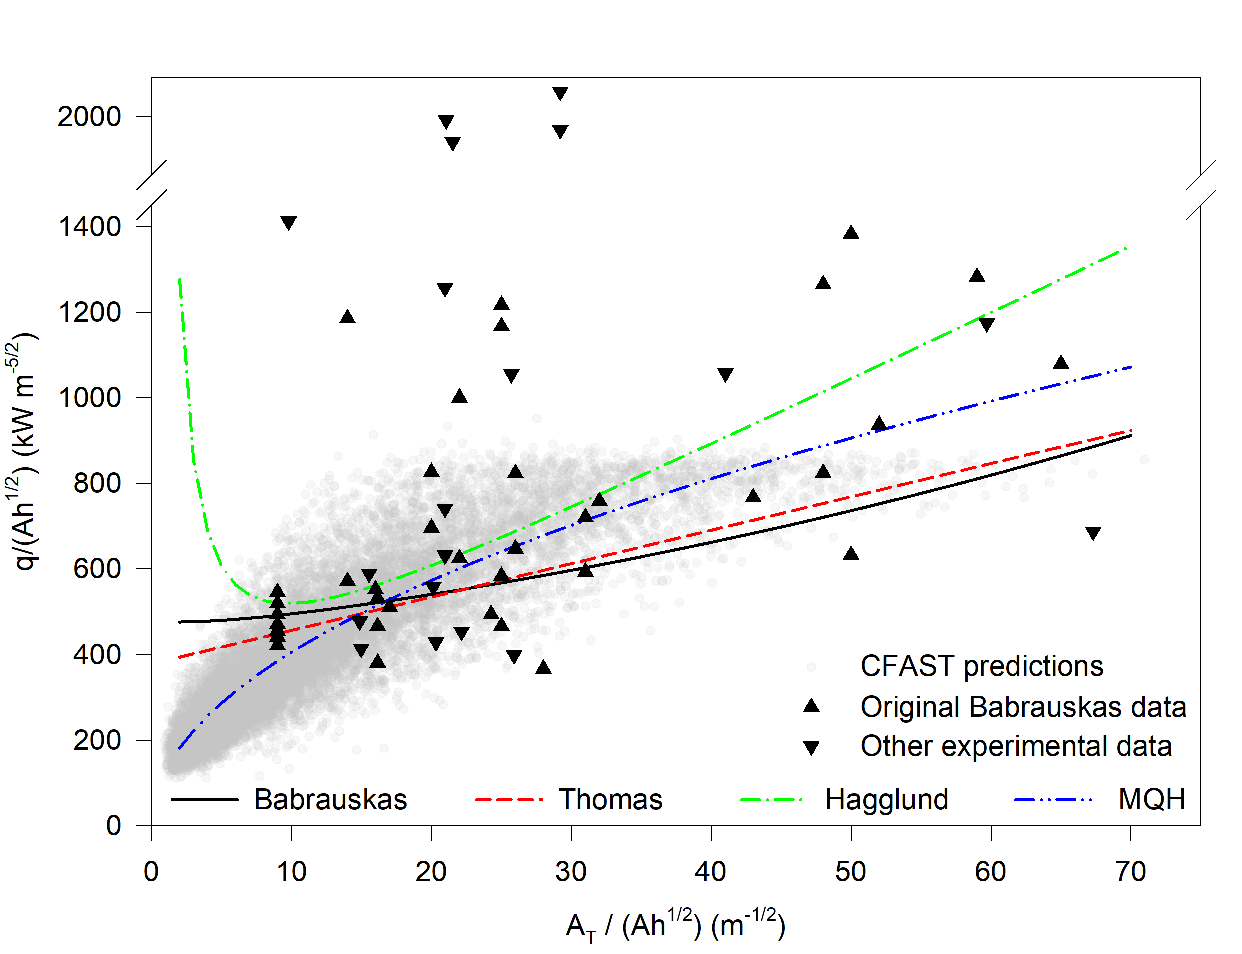
\includegraphics[width=6.0000in]{FIGURES/flashover.pdf}\\
\end{center}
\caption{Comparison of correlations, CFAST predictions, and experimental data for the prediction of flashover in a compartment fire.}
 \label{figValidFlashover}
\end{figure}

As with some of the experimental data defining flashover as an upper layer temperature reaching 600 $^{\circ}$C, many experimental measures were reported as peak values rather than minimum values necessary to achieve flashover. Thus, ideally all the predictions should provide a lower bound for the experimental data. Indeed, this is consistent with the graph -- the vast majority of the experimental observations lie above the correlations and model predictions. For a considerable range in the ratio \asqh, the correlations of Babrauskas \cite{Valid:Babrauskas_Flashover} Thomas \cite{Thomas:1981fk}, and the MQH correlation of McCaffrey et al. \cite{McCaffrey:1981uq} provide similar estimates of the minimum energy required to produce flashover. The estimates of H\"{a}gglund \cite{Hagglund:1980} yields somewhat higher estimates for values of \asqh  \, greater than 20 m$^{-1/2}$.

The results from the CFAST model for this single compartment scenario provide similar results to the experiments and the correlations for most of the range of \asqh. For small values of \asqh, the CFAST values rise somewhat above the values from the correlations. These small values of \asqh \, result from either very small compartments (small $A_T$) or very large openings (large \asqh), both of which stretch the limits of the assumptions inherent in the model. For very small compartments, radiation from the fire to the compartment surfaces becomes more important, enhancing the conductive heat losses through the walls. However, the basic two-zone assumption may break down as the room becomes very small. For very large openings, the calculation of vent flow via an orifice flow coefficient approach is likely inaccurate. Indeed, for such openings, this limitation has been observed experimentally \cite{Valid:Babrauskas_Flashover}. The estimates are close to the range of uncertainty shown by the correlations which also diverge at very small values of \asqh.

Perhaps most significant in these comparisons is that all the simple correlations provide estimates similar to the CFAST model and all the models are consistent with a wide range of experimental data. For this simple scenario, little is gained with the use of the more complex models. For more complicated scenarios, the comparison may not be as simple.

\section{Comparisons of CFAST with Actual Fires}

There are numerous cases of CFAST being used to adjudicate legal disputes. Since these are discussed in courts of law, there is a great deal of scrutiny of the modeling, assumptions, and results. Most of these simulations and comparisons are not available in the public literature. A few of the cases which are available are discussed below. The metric for how well the model performed is its ability to reproduce the time-line as observed by witnesses and the death of occupants or the destruction of property as was used in evidence in legal proceedings.

As mentioned in section \ref{secMultipleCompartments}, Levine and Nelson describe the use of FAST for understanding the deaths of two adults in a residence in Sharon, Pennsylvania in 1987 \cite{Valid:Levine}. The paper compared the evidence of the actual fire, a full scale mockup done at NIST and the results from FAST (version 18) \cite{Jones:1985} and Harvard VI \cite{Rockett:1985}. The most notable shortcoming of the models was the lower than actual temperatures in the bedrooms, caused by loss of heat through the fire barriers. This led to the improvement in CFAST in the mid-90s to couple compartments together so that both horizontal and vertical heat transfer can occur to adjacent compartments.

Bukowski used CFAST version 3.1 to analyze a fire in New York City \cite{Bukowski:1996} in 1994 which resulted in the death of three fire fighters. The CFAST model was able to reproduce the observed conditions and supported the theory as to how the fire began and the cause of death of the three fire fighters.

Chow describes the use and comparison of CFAST simulations with a 1996 high rise building fire in Hong Kong \cite{Chow:1996}. CFAST simulations were performed to help understand the probable fire environment under different conditions. Three simulations were performed to study the consequences of a fire starting in the lift shaft. Smoke flow in the simulations qualitatively matched those observed during the incident.

In the early morning hours of March 25,1990 a tragic fire took the lives of 87 persons at a neighborhood club in the Bronx, New York \cite{Bukowski:1992}. The New York City Fire Department requested the assistance of the NIST Center for Fire Research (CFR) in understanding the factors which contributed to this high death toll and to develop a strategy that might reduce the risk of a similar occurrence in the many similar clubs operating in the city. The simulation showed the potential for development of untenable conditions within the club and particularly in the single exit stairway.


\section{Comparisons of CFAST for Special Applications}

There are several sets of comparisons used in the development of the model or specific applications beyond those discussed more generally above.

\subsection{Nuclear Facilities}

Floyd validated CFAST version 3.1 by comparing the modeling results with measurements from fire tests at the Heiss-Dampf Reaktor (HDR) facility \cite{Floyd:2002}. The structure was originally the containment building for a nuclear power reactor in Germany. The cylindrical structure was 20 m in diameter and 50 m in height topped by a hemispherical dome 10 m in radius. The building was divided into eight levels. The total volume of the building was approximately 11 000 m$^3$. From 1984 to
1991, four fire test series were performed within the HDR facility. The T51 test series consisted of 11 propane gas tests and three wood crib tests. To avoid permanent damage to the test facility, a special set of test rooms were constructed, consisting of a fire room with a narrow door, a long corridor wrapping around the reactor vessel shield wall, and a curtained area centered beneath a maintenance hatch. The fire room walls were lined with fire brick. The doorway and corridor walls had the same construction as the test chamber. Six gas burners were mounted in the fire room. The fuel source was propane gas mixed with 10 \% air fed at a constant rate to one of the six burners.

In general, the comparison between CFAST and the HDR results was seen as `good' by the author, with two exceptions. The first is the over estimate of the temperature of the upper layer, typically within about 15 \% of the experimental measurements. This is common and generally results from using too low a value for the production of soot, water (hydrogen) and carbon monoxide. The other exception consists of predictions in spaces where the zone model concept breaks down, for example in the stairways between levels. In this case, CFAST has to treat the space either in the filling mode (two layer approximation) or as a fully mixed zone (using the SHAFT option). Neither is quite correct, and in order to understand the condition in such spaces in detail (beyond the transfer of mass and energy), a more detailed computational fluid dynamics model must be used, for example,  the Fire Dynamics Simulator (FDS) \cite{FDS_Tech_Guide_5}.

The U.S. Nuclear Regulatory Commission (NRC) performed an extensive verification and validation of several fire models commonly used in nuclear power plant applications \cite{NRCNUREG1824}.  These models included simple spreadsheet calculations, zone models (including CFAST), and CFD models. The results of this study are presented in the form of relative differences between fire model predictions and experimental data for fire modeling attributes such as temperature or heat flux that are important to NPP fire modeling applications.  These relative differences are affected by the capabilities of the models, the availability of accurate applicable experimental data, and the experimental uncertainty of these data. Evaluation of the two-zone models showed that the models simulated the experimental results within experimental uncertainty  for many of the parameters of interest. The reason for this may be that the relatively simple experimental configurations selected for this study conform well to the simple two-layer assumption that is the basis of these models.

While the relative differences sometimes show agreement for many parameters, they also show both under-prediction and over-prediction in some circumstances, most notably when conditions vary within a compartment or detailed local conditions are important to accurate prediction (for example, plume temperature or heat flux near to the fire source). The results and comparisons included the the NRC study are included in this report for the current version of CFAST.

\subsection{Small Compartments}

As an implementation of the zone model concept, CFAST is applicable to a wide range of scenarios. One end of this spectrum are small compartments, one to two meters on a side. Several research efforts have looked at small scale validation. There are three papers by Chow \cite{Lui:2003,Chow:1995,Chow:1992} which examine this issue. The first is the use of an electric heater with adjustable thermal power output was to verify temperature predictions by CFAST version 3.1. The second was closed chamber fires studied by burning four types of organic liquids, namely ethanol, N-heptane, and kerosene. The burning behavior of the liquids was observed, and the hot gas temperature measured. These behaviors along with the transient variations of the temperature were then compared with those predicted by the CFAST model. Finally, in another series of experiments, three zone models, one of which was CFAST, were evaluated experimentally using a small fire chamber. Once again, liquid fires were chosen for having better control on the mass loss rate. The results on the development of smoke layer and the hot gas temperature predicted by the three models were compared with those measured experimentally. According to Chow, `fairly good agreement' was found if the input parameters were carefully chosen.

\subsection{Railway and Vehicle Tunnels}

Altinakar et al. \cite{Altinakar:1997} used a \emph{modified version} of CFAST for predicting fire development and smoke propagation in vehicle or railroad tunnels. The two major modifications made to the model dealt with mixing between the upper and lower layers and friction losses along the tunnel. The model was tested by simulating several full-scale tests carried out at memorial Tunnel Ventilation Test Program in West Virginia, and the Offeneg Tunnel in Switzerland. His article compares simulated values of temperature, opacity and similar sensible quantities with measured values and discusses the limits of the applicability of zone models for simulating fire and smoke propagation in vehicle and railroad tunnels.

Peacock et al. \cite{Peacock:2004} compared times to untenable conditions determined from tests in a passenger rail car with those predicted by CFAST for the same car geometry and fire scenarios. For a range of fire sizes and growth rates, they found agreement that averaged approximately 13~\%.

\subsection{Non-Uniform Compartments}

In January 1996, the U.S. Navy began testing how the CFAST model would perform when tasked with predicting shipboard fires. These conditions include mass transport through vertical vents (representing hatches and scuttles), energy transport via conduction through decks, improvement to the radiation transport sub-model, and geometry peculiar to combat ships. The purpose of this study was to identify CFAST limitations and develop methods for circumnavigating these problems \cite{Hoover:2001}. A retired ship representing the forward half of a {USS} Los Angeles class submarine was used during this test series. Compartments in combat ships are not square in floor area, nor do they have parallel sides.

Application of CFAST to these scenarios required a direct integration of compartment cross-sectional area as a function of height to correctly interpret the layer interface position and provide correct predictions for flow through doors and windows (vertical vents). This required user specification of the area as a function of height to provide a description for the model to use.



\chapter{Verification}

The terms {\em verification} and {\em validation} are often used interchangeably to mean the process of checking the accuracy of a numerical model. For many, this entails comparing model predictions with experimental measurements. However, there is now a fairly broad-based consensus that comparing model and experiment is largely what is considered {\em validation}. So what is {\em verification}? ASTM~E1355~\cite{CFAST:ASTM:E1355}, ``Standard Guide for Evaluating the Predictive Capability of Deterministic Fire Models,'' defines verification as
\begin{quote}
The process of determining that the implementation of a calculation method accurately represents the developer's conceptual description of the calculation method and the solution to the calculation method.
\end{quote}
and it defines validation as
\begin{quote}
The process of determining the degree to which a calculation method is an accurate representation of the real world from the perspective of the intended uses of the calculation method.
\end{quote}
Simply put, verification is a check of the math; validation is a check of the physics. If the model predictions closely match the results of experiments, using whatever metric is appropriate, it is assumed by most that the model suitably describes, via its mathematical equations, what is happening. It is also assumed that the solution of these equations must be correct. So why do we need to perform model verification? Why not just skip to validation and be done with it? The reason is that rarely do model and measurement agree so well in all applications that anyone would just accept its results unquestionably. Because there is inevitably differences between model and experiment, we need to know if these differences are due to limitations or errors in the numerical solution, or the physical sub-models, or both.

Whereas model validation consists mainly of comparing predictions with experimental measurements, as documented later in this guide, model verification consists of a much broader range of activities, from checking the computer program itself, to comparing calculations to analytical (exact) solutions, to understanding the impact on model outputs from a range of different model inputs.

A series of verification test cases follow, examining the energy balance, mass balance, ventilation, heat transfer and sprinkler effects modeled by CFAST. These test cases are routinely run to ensure the calculations in the model are correct for a range of simple calculations where analytical solutions exist. The energy and mass balance examples test the underlying fundamental equations that determine conditions within a compartment in the model. The ventilation examples test the flow of gases between compartments through doors, windows, holes in floors/ceilings, and mechanical ventilation systems.  The heat transfer examples test the flow of energy through walls of compartments or to user-defined objects within a compartment. The sprinkler example tests the algorithm used to simulate the response of heat detectors and fire sprinklers in CFAST.  For each of the examples, an analytical solution is presented and compared to the results of a matching CFAST simulation.


\section{Energy}
\label{energy_balance}
For most of the examples presented in this section, the same basic geometry is used, a single 5~m by 5~m by 5~m compartment.

\subsection{Temperature Equilibrium via Heat Conduction}
\label{basic_tempequilib}

As a simple test of the energy balance, raising the external temperature of the base case compartment from an initial condition of 20~\degc to 25~\degc allows the internal temperature to equilibrate to the exterior. From the ideal gas law, the pressure inside the compartment is expected to rise to
\begin{equation}
   P_{\rm final} = P_{\rm initial} \; \frac{T_{\rm final}}{T_{\rm initial}} = 101325 \; {\rm Pa} \times \frac{298.15 \; {\rm K}}{293.15 \; {\rm K}} = 103053 \; {\rm Pa} \label{eq:Temperature_Equilibrium}
\end{equation}
or a final pressure rise of 1728 Pa.  Figure \ref{fig:Temperature_Equilibrium} shows the simulated conditions for this test, which are consistent with the expected results..

\begin{figure}[!ht]
\begin{tabular*}{\textwidth}{l@{\extracolsep{\fill}}r}
\includegraphics[width=3.0in]{SCRIPT_FIGURES/Verification/basic_tempequilib_temp} &
\includegraphics[width=3.0in]{SCRIPT_FIGURES/Verification/basic_tempequilib_pres}
\end{tabular*}
\caption[Results of the test case {\ct basic\_tempequilib.in}]{Interior temperature and pressure in equilibrium with the exterior in the case {\ct basic\_tempequilib.in}.}
\label{fig:Temperature_Equilibrium}
\end{figure}

\subsection{Temperature Equilibrium via a Window}
\label{basic_tempequilib_window}

Now an open window is added to the compartment, with an exterior temperature of 25~\degc. Figure~\ref{fig:Temperature_Equilibrium_With_Window} shows the interior conditions coming into equilibrium with the exterior, which are consistent with the expected results..

\begin{figure}[!ht]
\begin{tabular*}{\textwidth}{l@{\extracolsep{\fill}}r}
\includegraphics[width=3.0in]{SCRIPT_FIGURES/Verification/basic_tempequilib_window_temp} &
\includegraphics[width=3.0in]{SCRIPT_FIGURES/Verification/basic_tempequilib_window_pres}
\end{tabular*}
\caption[Results of the test case {\ct basic\_tempequilib\_window.in}]{Interior temperature and pressure in equilibrium with the exterior in the case {\ct basic\_tempequilib\_window.in}.}
\label{fig:Temperature_Equilibrium_With_Window}
\end{figure}

\subsection{Temperature Equilibrium via a Window at a High Elevation}
\label{basic_tempequilib_window_elevation}

With the exterior temperature still set to 25~\degc, the elevation is raised to 1500~m, approximately the average elevation of Idaho.  Since CFAST calculations are relative to the exterior ambient, conditions are expected to be identical to the previous examples and equilibrate to those of the exterior. Figure \ref{fig:Temperature_Equilibrium_Elevation} shows the simulated conditions for the test case, which are consistent with the expected results..

\begin{figure}[!ht]
\begin{tabular*}{\textwidth}{l@{\extracolsep{\fill}}r}
\includegraphics[width=3.0in]{SCRIPT_FIGURES/Verification/basic_tempequilib_window_elevation_temp} &
\includegraphics[width=3.0in]{SCRIPT_FIGURES/Verification/basic_tempequilib_window_elevation_pres}
\end{tabular*}
\caption[Results of the test case {\ct basic\_tempequilib\_window\_elevation.in}]{Interior temperature and pressure in equilibrium with the exterior in the case {\ct basic\_tempequilib\_window\_elevation.in}.}
\label{fig:Temperature_Equilibrium_Elevation}
\end{figure}

\subsection{A Fire in a Single, Sealed Compartment with a Single Zone}
\label{sealed_test}

A 100~kW methane fire burns in a sealed compartment with no ventilation, adiabatic walls, and no radiative emission. A single zone simulation is run in which it is assumed that the entire volume is taken up by the upper layer.  From Eqs. (2.5) and (2.6) in the CFAST Technical Guide~\cite{CFAST_Tech_Guide_6}, the governing equation for the pressure and temperature of the single zone compartment are:
\begin{eqnarray}
   \frac{{\rm d} P}{{\rm d}t} &=& \frac{\gamma-1}{V} \, \dot{q}   \label{eq1}
 \\[0.1in]
   \frac{{\rm d} T}{{\rm d}t} &=& \frac{1}{c_p \, m} \left( \dot{q} - c_p \, \dot{m} \, T + V \, \frac{{\rm d} P}{{\rm d}t} \right)
   \label{eq2}
\end{eqnarray}
where $m$ is the total mass in the volume, $\dot{m}=\dm_{\rm f}$ is the mass flow rate of the fuel into the volume, and
$\dot{q}=\dot{Q} + c_p \, \dot{m}_{\rm f} \, T_{\rm f} $ is the heat release rate of the fire plus the heat flow rate of the fuel flowing into the volume.
Note that $\dot{m}$ and $\dot{q}$ are source terms, they are assumed to have this form for this test problem.

Eq.~(\ref{eq2}) can be shown to be equivalent to the first law of thermodynamics by first substituting ${\rm d}P/{\rm d}t$ from Eq.~(\ref{eq1}) and noting that $\gamma=c_p/c_v$ to obtain
\begin{eqnarray}
   \frac{{\rm d} T}{{\rm d}t} &=& \frac{1}{c_p \, m} \left( \dot{q} - c_p \, \dot{m} \, T +  (\gamma-1) \, \dot{q}\right)\\
   \label{eq3}
    &=& \frac{1}{c_p \, m} \left( \gamma\dot{q} - c_p \, \dot{m} \, T   \right)\\
    &=& \frac{1}{c_v \, m} \left( \dot{q} - c_v \, \dot{m} \, T   \right)\label{eq4}
\end{eqnarray}

\noindent Next, the first law of thermodynamics can be stated as
\begin{eqnarray}
\frac{\rm d}{{\rm d}t}\left(c_vmT\right) = \dot{q} - P\frac{{\rm d}V}{{\rm d}t}=\dot{q}\label{eq5}
\end{eqnarray}
since ${\rm d}V/{\rm d}t=0$ (for this case).
\noindent Expanding and solving for ${\rm d} T/{\rm d}t$ results in
\begin{eqnarray}
c_v\dot{m}T+c_vm\frac{{\rm d}T}{{\rm d}t} &= &\dot{q}\\
    \frac{{\rm d} T}{{\rm d}t}&=& \frac{1}{c_v \, m} \left( \dot{q} - c_v \, \dot{m} \, T   \right)
\end{eqnarray}
which is identical Eq.~(\ref{eq4}) and therefore equivalent to Eq.~(\ref{eq2}).

Since the right hand side of Eq.~(\ref{eq1}) is constant, it may be integrated to obtain the solution
\begin{equation}
P(t)=P_0+\frac{\gamma-1}{V}\,\dot{q}\,t \label{eq:soleq1}
\end{equation}
where $P_0$ is the initial pressure.  A solution for Eq.~(\ref{eq2}) may be found by using Eq.~(\ref{eq:soleq1}) and the ideal gas law to obtain
\begin{equation}
T(t)=\frac{V\,P(t)}{R\,m(t)}\label{eq:soleq2}
\end{equation}
where $m(t)=m_0+\dot{m}\,t$, $m_0=\frac{P_0\,V}{R\,T_0}$, is the initial mass, $T_0$ is the initial pressure and $R=c_p-c_v$.

Figure~\ref{fig:Analytical_Closed_Compartment} includes comparisons of the temperature and pressure as predicted by CFAST and the analytic solutions given
in Eqs.~(\ref{eq:soleq1}) and (\ref{eq:soleq2}).

\begin{figure}[!ht]
\begin{tabular*}{\textwidth}{l@{\extracolsep{\fill}}r}
\includegraphics[width=3.0in]{SCRIPT_FIGURES/Verification/sealed_test_temp} &
\includegraphics[width=3.0in]{SCRIPT_FIGURES/Verification/sealed_test_pres}
\end{tabular*}
\caption[Results of the test case {\ct sealed\_test.in}]{Temperature and pressure rise due to a fire in a closed compartment. The case is called {\ct sealed\_test.in}.}
\label{fig:Analytical_Closed_Compartment}
\end{figure}

\subsection{A Fire in a Single, Sealed Compartment with Two Zones}
\label{sealed_test_2_layers}

Consider now the same case as in Section~\ref{sealed_test}, but now with two zones rather than one. The compartment pressure ought to be the same as before, and the upper layer temperature ought to converge to the single layer temperature as seen in Fig.~\ref{fig:Analytical_Closed_Compartment2}.
\begin{figure}[!ht]
\begin{tabular*}{\textwidth}{l@{\extracolsep{\fill}}r}
\includegraphics[width=3.0in]{SCRIPT_FIGURES/Verification/sealed_test_2_layers_temp} &
\includegraphics[width=3.0in]{SCRIPT_FIGURES/Verification/sealed_test_2_layers_pres}
\end{tabular*}
\caption[Results of the test case {\ct sealed\_test\_2\_layers.in}]{Hot gas layer temperature and pressure rise due to a fire in a closed compartment with two zones. The case is called {\ct sealed\_test\_2\_layers.in}.}
\label{fig:Analytical_Closed_Compartment2}
\end{figure}

\clearpage


\section{Mass}
\label{mass_conservation}
\label{mass_balance}

\subsection{A Fire in a Single, Sealed Compartment}
\label{sec:spec1}
\label{species_mass_1}

A methane fire burns in a sealed compartment of dimension 5~m by 6~m by 3~m. The heat release rate ramps up linearly to 1~kW in 30~s, then remains steady for 5~min, and then ramps down linearly to 0 in 30~s. The total energy released is 330~kJ, and the total mass of fuel consumed is
\begin{equation}
  \frac{ 330 \; {\rm kJ} }{ 50000 \; {\rm kJ/kg} } = 0.00660 \; {\rm kg}
\end{equation}
where the heat of combustion of methane is taken to be 50 000 kJ/kg. For complete combustion of methane, the combustion chemistry is given by
\begin{equation}
   \mathrm{CH_4 + 2 \, O_2 \to CO_2 + 2 \, H_2O}
   \label{eq:Methane_Combustion}
\end{equation}
The molecular weight of CH$_4$ is 16~g/mol and CO$_2$ is 44~g/mol; thus, the total mass of CO$_2$ produced by the fire is
\begin{equation}
   m_{\rm CO_2} = 0.0066 \; {\rm kg} \times  \frac{ 44 \; {\rm g/mol} }{ 16 \; {\rm g/mol} } = 0.01815 \; {\rm kg}
\end{equation}
The molecular weight of H$_2$O is 18~g/mol; thus, the total mass of H$_2$O produced by the fire is
\begin{equation}
   m_{\rm H_2O} = 0.0066 \; {\rm kg} \times  \frac{ 2(18) \; {\rm g/mol} }{ 16 \; {\rm g/mol} } = 0.01485 \; {\rm kg}
\end{equation}
CFAST predicts that the final mole fractions of O$_2$, CO$_2$ and H$_2$O in the upper layer are 0.2069, 0.00012 and 0.00024, respectively (calculated by the model consistent with eq. \ref{eq:Methane_Combustion}; see \cite{CFAST_Tech_Guide_7} for details of the combustion chemistry calculations in CFAST). The remainder is N$_2$, whose mole fraction is 0.7927. These mole fractions can be converted to mass fractions by
\begin{equation}
Y_k = \frac{X_{k} M_{k}}{\sum_{i=1}^N X_{i}M_{i}}
\end{equation}
The mass of the upper layer can be calculated from the equation of state:
\begin{equation}
m_{\rm u} = \frac{P \, V}{R \, T} \quad ; \quad R = \frac{\gamma-1}{\gamma} \, c_p \approx 289.14 \; {\rm  \frac{J}{kg \cdot K}}
\end{equation}
The mass of CO$_2$ and H$_2$O produced is given by
\begin{equation}
m_{k} = m_{\rm u} \, Y_{k}
\end{equation}
Figure~\ref{specmass1} shows the resulting product masses, which are consistent with the expected results.

\begin{figure}[!ht]
\centering
\includegraphics[width=3.0in]{SCRIPT_FIGURES/Verification/species_mass_1}
\caption[Results of the test case {\ct species\_mass\_1.in}]{Expected and predicted masses of CO$_2$ and H$_2$O for the case {\ct species\_mass\_1.in}.}
\label{specmass1}
\end{figure}


\subsection{A Fire in a Compartment Connected to Another via a Door}
\label{sec:spec2}
\label{species_mass_2}

The same natural gas fire described in Section~\ref{sec:spec1} burns in a compartment of dimension 2~m by 5~m by 8~m which is connected to another compartment of dimension 5~m by 3~m by 8~m. A doorway connects the compartments, which has a width of 1~m and a height of 6~m. Because the fire and the fuel source have not changed, the theoretical calculations for the mass of CO$_2$ and H$_2$O produced will remain the same. The remaining portion of the problem is approached in the same manner, but since there are two compartments, the mass of CO$_2$ and H$_2$O produced in each layer of each compartment must be individually calculated and then summed together to produce the net yields of CO$_2$ and H$_2$O. Figure~\ref{specmass2} shows the resulting product masses, which are consistent with the expected results.
\begin{figure}[!ht]
\centering
\includegraphics[width=3.0in]{SCRIPT_FIGURES/Verification/species_mass_2}
\caption[Results of the test case {\ct species\_mass\_1.in}]{Expected and predicted masses of CO$_2$ and H$_2$O for the case {\ct species\_mass\_2.in}.}
\label{specmass2}
\end{figure}

\subsection{A Fire in a Compartment Connected to Another via a Ceiling Vent}
\label{species_mass_3}

The same natural gas fire described in Section~\ref{sec:spec1} burns in a compartment of dimension 9~m by 5~m by 4~m which is connected to another compartment of dimension 9~m by 5~m by 2~m. The compartments are placed such that the second one is located directly above the first one. There is a square ceiling vent between the compartments that has an area of 4~m$^2$. This problem is approached in the same exact manner as in Section~\ref{sec:spec2} because the only difference between the two scenarios is the specific alignment of the compartments.
Figure~\ref{specmass2} shows the resulting product masses, which are consistent with the expected results.
\begin{figure}[!ht]
\centering
\includegraphics[width=3.0in]{SCRIPT_FIGURES/Verification/species_mass_3}
\caption[Results of the test case {\ct species\_mass\_3.in}]{Expected and predicted masses of CO$_2$ and H$_2$O for the case {\ct species\_mass\_3.in}.}
\label{specmass3}
\end{figure}

\subsection{A Fire in a Four Compartment Assembly}
\label{sec:specmass4}
\label{species_mass_4}
\label{species_mass_4_theoretical}
\label{species_mass_4_TP}

Four 4~m by 4~m by 4~m compartments are arranged such that two compartments are placed adjacent to one another and the following two compartments are placed directly on top of the first two. The same natural gas fire described in Section~\ref{sec:spec1} burns in the first compartment of this setup. After 2500~s, the wall between compartments one and two is removed, forcing the gases in the two rooms to mix. Next, at 5000~s, the wall between compartments three and four is removed. Lastly, at 7500~s, the ceiling of compartment four is removed, allowing the system to slowly return to ambient conditions. Figure~\ref{fig:specmass4} shows the resulting product masses in the structure before the outside vent is opened, which are consistent with the expected results.  Figure~\ref{fig:specmass4abcd} shows how the masses of CO$_2$ and H$_2$O in each compartment change with respect to time.
\begin{figure}[!ht]
\centering
\includegraphics[width=3.0in]{SCRIPT_FIGURES/Verification/species_mass_4}
\caption[Results of the test case {\ct species\_mass\_4.in}]{Expected and predicted masses of CO$_2$ and H$_2$O for the case {\ct species\_mass\_4.in}.}
\label{fig:specmass4}
\end{figure}

\begin{figure}[!ht]
\begin{tabular*}{\textwidth}{l@{\extracolsep{\fill}}r}
\includegraphics[width=3.0in]{SCRIPT_FIGURES/Verification/species_mass_4a} &
\includegraphics[width=3.0in]{SCRIPT_FIGURES/Verification/species_mass_4b} \\
\includegraphics[width=3.0in]{SCRIPT_FIGURES/Verification/species_mass_4c} &
\includegraphics[width=3.0in]{SCRIPT_FIGURES/Verification/species_mass_4d}
\end{tabular*}
\caption[Results of the test case {\ct species\_mass\_4.in}]{Expected and CFAST calculated values for the masses of CO$_2$ and H$_2$O in each compartment of a four room test case {\ct species\_mass\_4.in}.}
\label{fig:specmass4abcd}
\end{figure}

\subsection{Product Yields}
\label{methane_flame}

A simple 5 kW methane flame with 10~\% CO yield is burned inside a closed 5~m x 5~m x 5~m compartment for 100~s. Initially, the relative humidity within the compartment is zero. The total mass of CO$_2$, H$_2$O and CO produced is calculated. The combustion of a hydrocarbon fuel is described by the following single-step reaction:
\be
   \mathrm{C_{n_\C}H_{n_H}} +  \nu_\OTWO \, \mathrm{O_2}  \rightarrow   \nu_\COTWO \, \mathrm{CO_2} + \nu_\HTWOO \, \mathrm{H_2O} \; + \; \nu_\CO \, \mathrm{CO}
\ee
where
\begin{eqnarray}
    \nu_\CO &=& \frac{M_\F}{M_\CO} \; y_\CO \\[.1in]
    \nu_\COTWO &=& \mathrm{n_\C} - \nu_\CO \\[.1in]
    \nu_\HTWOO &=& \frac{\mathrm{n_\Hy}}{2} \\[.1in]
    \nu_\OTWO  &=& \nu_\COTWO + \frac{\nu_\HTWOO + \nu_\CO}{2}
\end{eqnarray}

With a total mass of methane burned of 0.01 kg (5 kW / 50000 MJ/kg $\times$ 100 s), 0.026 kg of CO$_2$, 0.022 kg of H$_2$O, and 0.001 kg of CO are produced by the fire. The following figure compares the mass of the three combustion products to their expected values.

\begin{figure}[ht]
\centering
\includegraphics[width=3.0in]{SCRIPT_FIGURES/Verification/methane_flame}
\caption[Results of the test case {\ct methane\_flame\_simple.in}]{Expected and CFAST calculated values for the masses of CO, CO$_2$, and H$_2$O in a one room test case {\ct methane\_flame\_simple.in}.}
\label{fig_methane_flame_yields}
\end{figure}

\clearpage

\clearpage


\section{Ventilation}
\label{ventilation}

\subsection{Air Flow Through a Single Compartment}
\label{ventilation_1}

The setup for this test case includes a 5~m by 5~m by 3~m compartment that contains a mechanical vent and a wall vent. Air is pumped into a single compartment through a 1~m by 1~m mechanical vent, at a rate of 0.01~m$^3$/s. The air is allowed to exit the compartment through a 1~cm by 1~cm vent located on the opposite side of the compartment. The governing equation for the change in pressure in the compartment is \cite{Emmons:SFPE}:
\begin{equation}
\Delta{P} = \frac{1}{2\rho}\brackets{\frac{\dot{m}}{CA}}^2
\end{equation}
where $\rho$ , $\dot{m}$ and $C$ are consistent with CFAST calculations
\begin{equation}
\rho = \frac{P}{RT} \quad ; \quad  \dot{m} = \rho_{\infty} \dot{V} \quad ; \quad C = 0.70
\end{equation}
Figure~\ref{fig:vent1} shows how the pressure changes as air flows through the compartment.

\begin{figure}[!ht]
\centering
\includegraphics[width=3.0in]{SCRIPT_FIGURES/Verification/ventilation_1_pressure}
\caption[Results of the test case {\ct ventilation\_1.in}]{Expected and CFAST calculated values for pressure of the compartment for the case {\ct ventilation\_1.in}.}
\label{fig:vent1}
\end{figure}



\subsection{Steady-State Air Flow}
\label{sec:vent2}
\label{ventilation_2}

A similar setup to the one used in Section~\ref{sec:specmass4} is employed here. A fan blows air into the first compartment, on the ground floor, at a rate of 1~m$^3$/s and then continues to the second compartment after passing through a doorway. The air then travels to the third compartment by passing through a ceiling vent with an area of 3~m$^2$ and continues to compartment four through another doorway. Air is finally extracted from compartment four at a rate of 1~m$^3$/s. Figure~\ref{ventilation_2TP} shows  temperature and pressure as the air flows through the fourth compartment. As expected, the temperature remains at ambient conditions and flow in the lower compartment matches flow out the upper compartment

\begin{figure}[!ht]
\begin{tabular*}{\textwidth}{l@{\extracolsep{\fill}}r}
\includegraphics[width=3.0in]{SCRIPT_FIGURES/Verification/ventilation_2_temperature} &
\includegraphics[width=3.0in]{SCRIPT_FIGURES/Verification/ventilation_2_flow}
\end{tabular*}
\caption[Results of the test case {\ct ventilation\_2.in}]{Expected and CFAST calculated values for temperature and mass flow for the case {\ct ventilation\_2.in}.}
\label{ventilation_2TP}
\end{figure}


\subsection{Non Steady-State Air Flow}
\label{ventilation_3}

The same setup that was constructed in Section~\ref{sec:vent2} is used again in this scenario. All vents and fans are the same as in the previous case, except the fan in the fourth compartment has been converted to a round ceiling vent with an area of 4~m$^2$. Initially, all of the vents are closed and air is pumped into the first compartment at a rate of 1~m$^3$/s, for a period of 15~s. After 15~s pass, the fan is shut off. Then, at 200~s, the door between compartments one and two opens completely. Next, at 500~s, the vent between compartments two and three opens completely. At 700~s, the door between compartments three and four opens completely. Finally, at 1000~s, the ceiling vent in compartment four opens completely. Figure~\ref{ventilation_3TP} shows how temperature and pressure change as the air flows through the first compartment.

\begin{figure}[!ht]
\begin{tabular*}{\textwidth}{l@{\extracolsep{\fill}}r}
\includegraphics[width=3.0in]{SCRIPT_FIGURES/Verification/ventilation_3_temperature} &
\includegraphics[width=3.0in]{SCRIPT_FIGURES/Verification/ventilation_3_pressure}
\end{tabular*}
\caption[Results of the test case {\ct ventilation\_3.in}]{Expected and CFAST calculated values for pressure and temperature of the first compartment for the case {\ct ventilation\_3.in}.}
\label{ventilation_3TP}
\end{figure}

\subsection{Velocity Profile of Air Flowing Through a Doorway}
\label{ventilation_4}

A 200~kW natural gas (methane) fire burns in a 5~m by 5~m by 5~m compartment, where the walls are assumed to be adiabatic. The heat release rate ramps up linearly to 200~kW in 30~s, then remains steady for 5.5~min. The compartment contains a 4~m by 1.5~m door that remains completely open throughout the simulation. The mass flow though each vertical segment of the doorway is given by:
\begin{equation}
\dot{m} = \int_b^t C \sqrt{2\rho\Delta{P(z)}} \, w\;\mathrm{d}z
\label{eq:mdot}
\end{equation}
where $C$ is the orifice coefficient taken to be 0.7, $\rho$ is the gas density of the upwind compartment, $w$ is the width of the doorway and $\Delta{P(z)}$ is the pressure across the interface at elevation $z$. Finally, $z = b$ and $z = t$ refer to the heights of the bottom and top of the vertical segment in the doorway through which the mass flow rate is being calculated. This equation can be analytically integrated to yield:
\begin{equation}
\dot{m} = {\rm sign} \brackets{\frac{\Delta P_t + \Delta P_b}{2}} \, \frac{2}{3} \, C \sqrt{2\rho} \, w \, (t-b)\frac{|\Delta P_t|^{3/2}-|\Delta P_b|^{3/2}}{|\Delta P_t|-|\Delta P_b|}
\end{equation}
The equation for the velocity profile of air traveling through the doorway can be produced after rearranging equation~\ref{eq:mdot}:
\begin{equation}
v(z) = \frac{\dot{m}}{\delta A \, \rho} = {\rm sign}(\Delta{P(z)}) \, C \sqrt{\frac{2|\Delta{P(z)}|}{\rho}}
\end{equation}
where $\delta A$ represents the infinitesimal area of the door segment and $\rho$ corresponds to the density of air at height $z$. Figure~\ref{fig:vel} shows how the velocity of air flowing through the doorway changes from the floor to the top of the doorway.

\begin{figure}[!ht]
\centering
\includegraphics[width=3.0in]{SCRIPT_FIGURES/Verification/ventilation_4_vel}
\caption[Results of the test case {\ct ventilation\_4.in}]{CFAST calculated velocity profile of air traveling through the doorway in test case {\ct ventilation\_4.in}.}
\label{fig:vel}
\end{figure}

\subsection{Flow Through Different Vent Types}
\label{VVent_Tests}

A fan is supplies air into a compartment at a constant rate of 0.1 m$^3$/s (0.12 kg/s). Vertical and horizontal natural flow vents connect this compartment to two other compartments stacked vertically.  Finally, the structure is vented to the outside by either a vertical or horizontal flow vent in the rooms removed from the one where air is supplied. Figure~\ref{fig:vvent} shows a sample of the mass flow through the vents.

\begin{figure}
\begin{center}
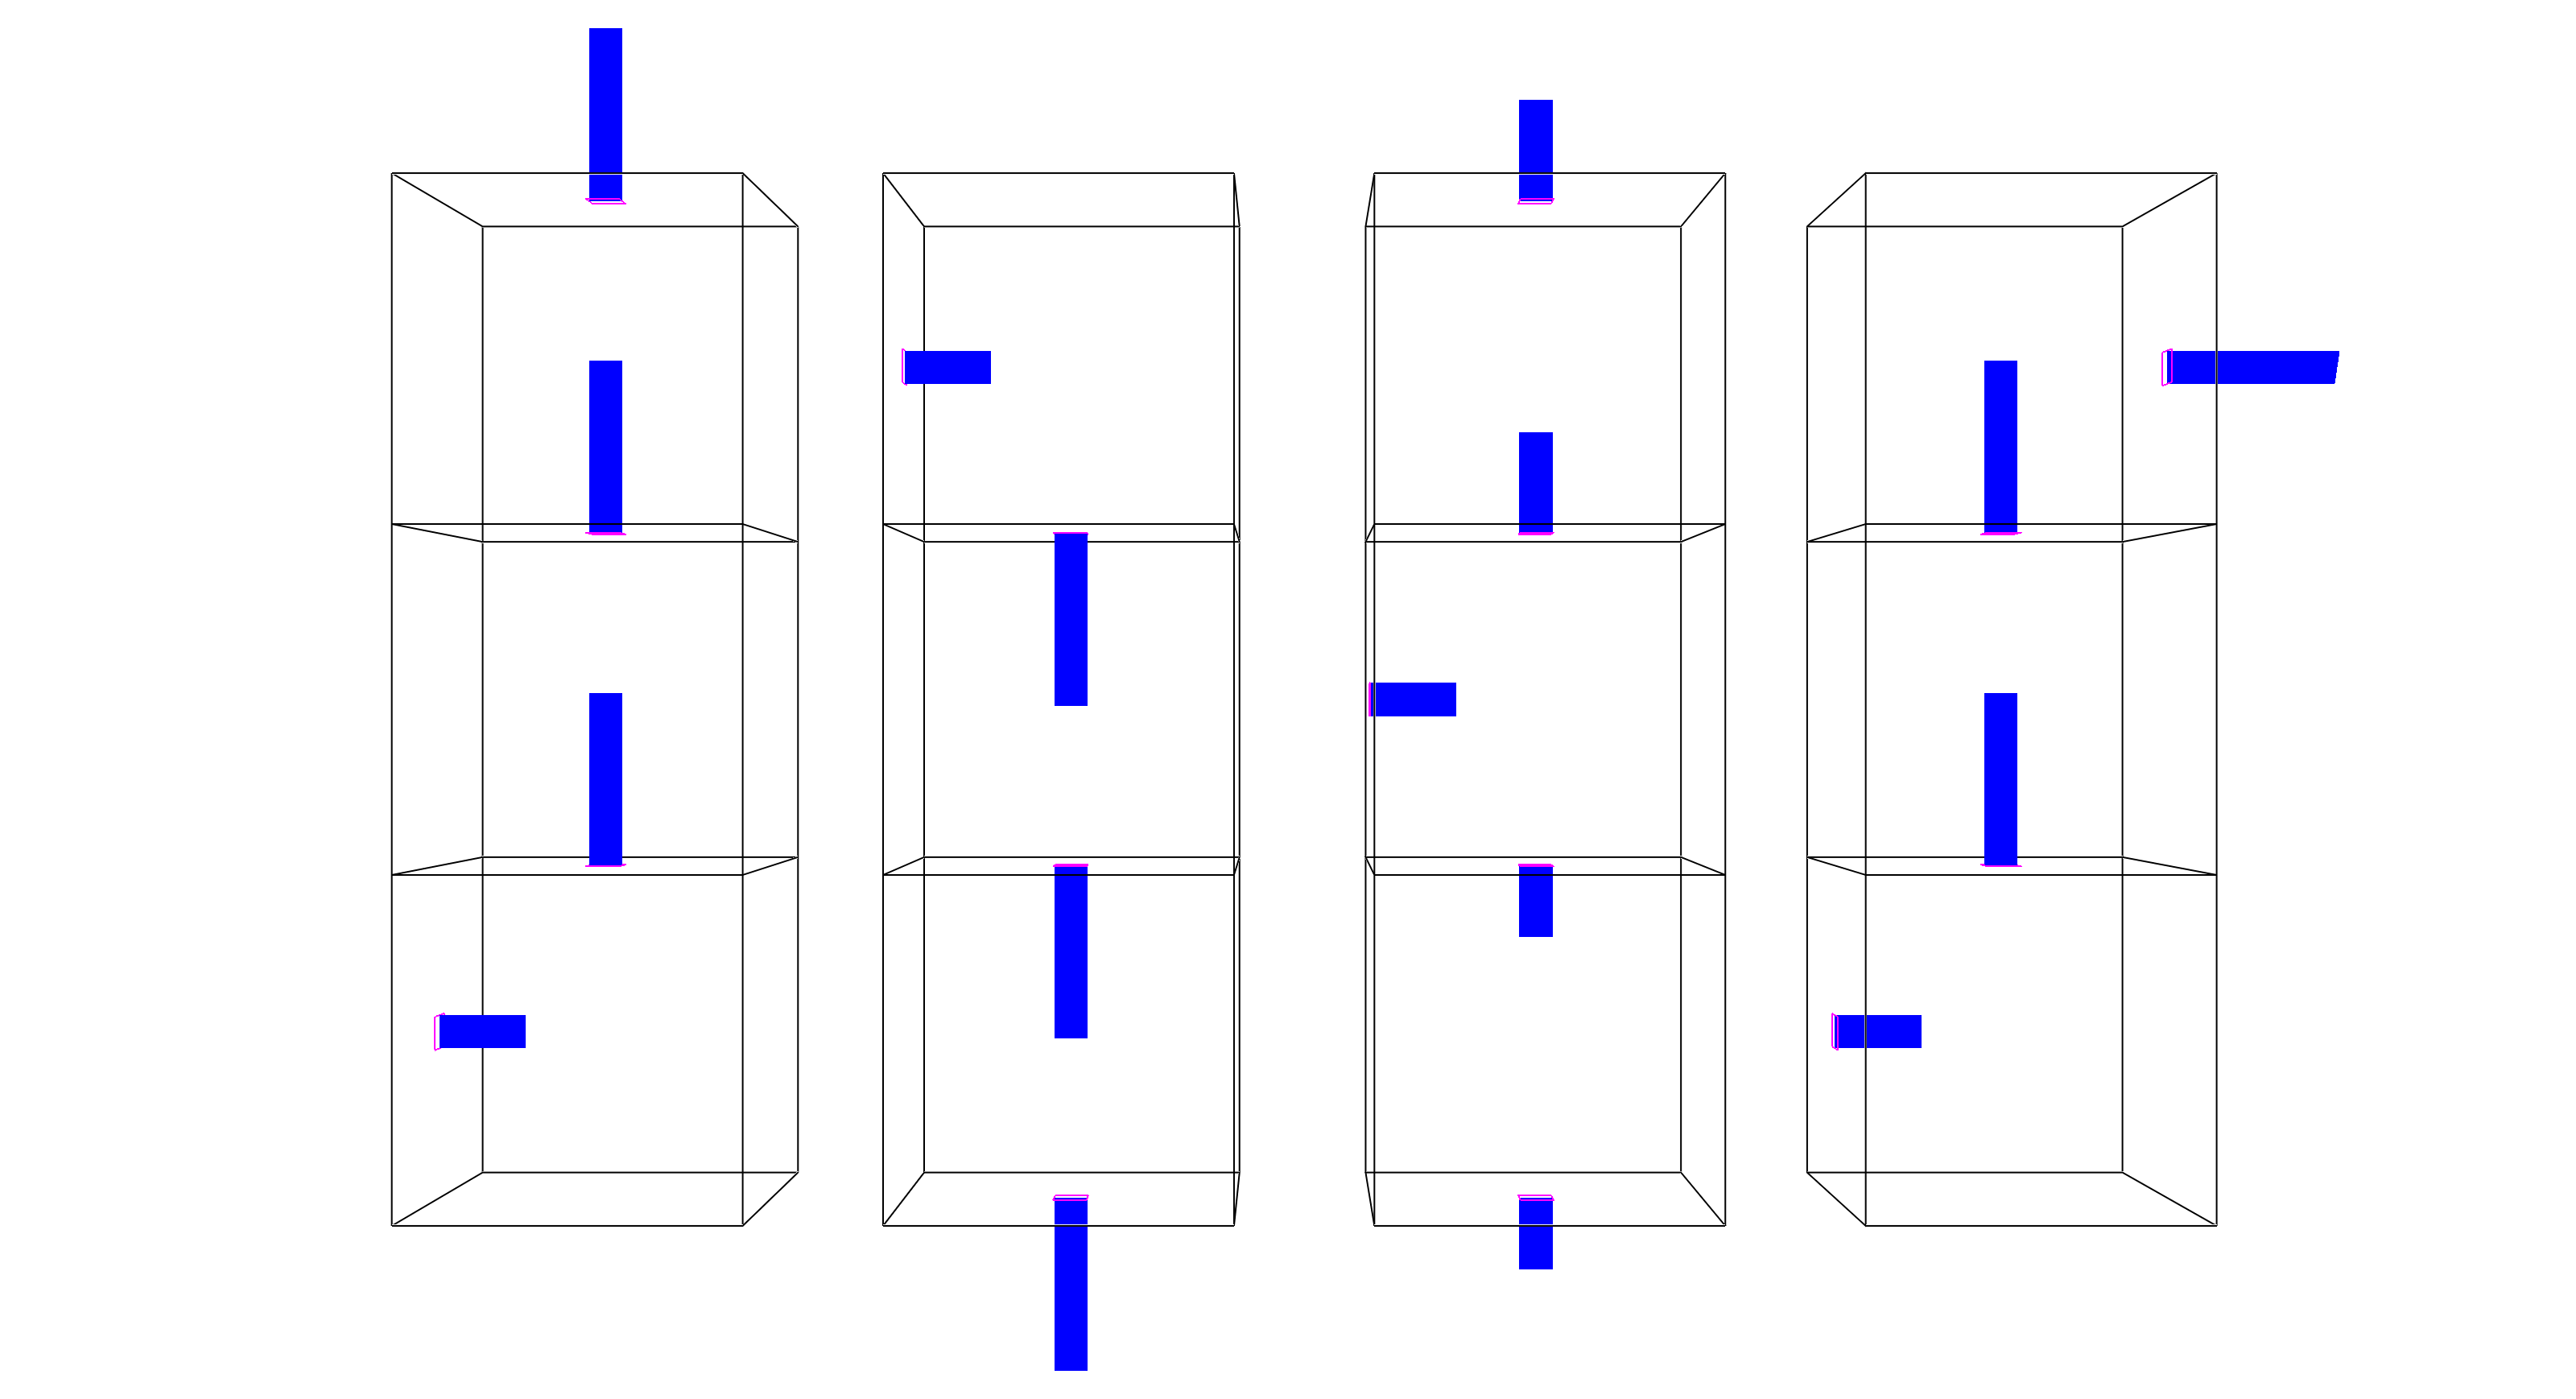
\includegraphics[height=3.0in]{FIGURES/Verification/VVent_Geom} \\
\includegraphics[width=3.0in]{SCRIPT_FIGURES/Verification/VVent_Tests}
\end{center}
\caption[Results of the test case {\ct VVent\_Tests.in}]{Expected and CFAST calculated values for mass flow through vents {\ct VVent\_Tests.in}.}
\label{fig:vvent}
\end{figure}

\section{Heat Transfer}
\label{radiation}

\subsection{Measuring the Temperature Change of a Thermally Thin Target}
\label{radiation_1}

A constant 10~kW natural gas (methane) fire burns in the center of a 15~m by 15~m by 15~m compartment. Because the purpose of this case is to test the point source radiation model and the heating of a thermally-thin target, there is a 20~m$^2$ vent located in the center of the ceiling to exhaust the smoke from the fire and maintain an ambient temperature lower layer. A 1.5~mm thick sheet of plain carbon steel is placed 2~m to the right of the fire. It is oriented directly at the fire. The target is heated by the thermal radiation from the fire, and it is cooled via convective and radiative loss. The net radiative heat transfer to the target is given by:
\begin{equation}
\dqr'' = \epsilon \frac{\chi_{\rm r} \, \dot{Q}}{4\pi \, r^2} + 2\epsilon \sigma ( T_{\rm g}^4 - T_{\rm s}^4)
\end{equation}
where $\epsilon$ is the emissivity of the target, $\chi_{\rm r}$ represents the radiative heat fraction of the fire, $\dot{Q}$ is the heat release rate of the fire, $r$ is the distance between the fire and the target and $\sigma$ is the Stefan-Boltzmann constant, which has a value of $5.67 \times 10^{-11}$~kW/(m$^2 \cdot$K$^4$). Additionally, $T_{\rm g}$ is the temperature of the gas surrounding the target and $T_{\rm s}$ is the temperature of the target's surface. The convective heat flux to a solid surface is governed by the following equations:
\begin{equation}
\dqc'' = h(T_{\rm g}-T_{\rm s}) \quad ; \quad  h = C|T_{\rm g} - T_{\rm s}|^{1/3}
\end{equation}
where $h$ is the convective heat transfer coefficient and $C$ is an empirical coefficient determined to be 1.31 for vertical targets \cite{Holman:1990}. In order to determine what the temperature of the target's surface will be at any given time, the following equation must be integrated \cite{Moss:1992}:
\begin{equation}
\frac{{\rm d} T}{{\rm d} t} = \frac{\dqr'' + 2\dqc''}{\delta \, \rho \, C_{\rm p}}
\end{equation}
where $\delta$, $\rho$ and $C_{\rm p}$ are the thickness, density and specific heat capacity of the target. The 2 denotes that both sides of the target cool via convection. Figure~\ref{fig:rad1} shows how the surface temperature of the target changes as the fire burns in the compartment.

\begin{figure}[!ht]
\centering
\includegraphics[width=3.0in]{SCRIPT_FIGURES/Verification/radiation_1_temp}
\caption[Results of the test case {\ct radiation\_1.in}]{Expected and CFAST calculated target surface temperature values for the case {\ct radiation\_1.in}.}
\label{fig:rad1}
\end{figure}

\subsection{Measuring the Temperature Change of a Cylindrical Target}
\label{radiation_2}

A 0.15~cm thick steel plate, a 2.5~cm thick steel plate and a 2.5~cm diameter steel rod are placed in a furnace\footnote{CFAST has an option to create a uniform temperature environment for diagnostic purposes. The option must be invoked by adding a special comment to the input file.} with uniform temperature of 500~$^\circ$C. The heat conduction equations normal to the surface of each plate and the rod, respectively, are:
\begin{equation}
\frac{\partial T}{\partial t} = \frac{k}{\rho c}\frac{\partial^2 T}{\partial x^2} \quad ; \quad \frac{\partial T}{\partial t} = \frac{k}{\rho c} \frac{1}{r} \frac{\partial}{\partial r} \left( r \frac{\partial T}{\partial r} \right)
\end{equation}
where $k$, $\rho$ and $c$ are the thermal conductivity, density and specific heat capacity of the target. At the surface of each plate and the rod, the respective boundary conditions are:
\begin{equation}
\dq'' = -k \frac{\partial T}{\partial x} \quad ; \quad \dq'' = k \frac{\partial T}{\partial r}
\end{equation}
where $\dq''$ is the sum of the net radiative and convective heat fluxes:
\begin{equation}
\dqr'' = \epsilon \sigma \brackets{ T_{\rm g}^4 - T_{\rm s}^4 } \quad ; \quad \dqc'' = h \brackets{T_{\rm g} - T_{\rm s}}  \quad ; \quad h = C|T_{\rm g} - T_{\rm s}|^{1/3}
\end{equation}
where $\epsilon$ is the emissivity of the target (taken here to be 1), $\sigma$ is the Stefan-Boltzmann constant, $T_{\rm g}$ is the temperature of the gas surrounding the target, $T_{\rm s}$ is the temperature of the target's surface, $h$ is the convective heat transfer coefficient, and $C$ is 1.31 for vertical targets. Figure~\ref{fig:rad2} shows how the surface temperature for each of the plates and the rod increases with respect to time.

\begin{figure}[!ht]
\centering
\includegraphics[width=3.0in]{SCRIPT_FIGURES/Verification/radiation_2_temp}
\caption[Results of the test case {\ct radiation\_2.in}]{Expected and CFAST calculated surface temperature values for three different types of targets for the case {\ct radiation\_2.in}.}
\label{fig:rad2}
\end{figure}

\subsection{Measuring Incident Heat Flux to Targets}
\label{radiation_3}

Consider a 2~m by 2~m by 4~m enclosure with black walls as shown in Figure~\ref{fig:rad3_1}. For a pure water vapor medium at 1~atm with wall and gas temperature being maintained at 726.85~$^\circ$C, the incident heat flux to target devices, along the line (X, 2~m, 4~m) on the top surface of the enclosure and the line (2~m, 1~m, Z) on the right surface, are obtained. Comparison between benchmark results (exact) reported from the literature \cite{Liu:1999} and results calculated by CFAST is made. Figure~\ref{fig:rad3_2} shows the incident heat flux to the target devices due to the emission from a hot medium and Figure~\ref{fig:rad3_3} shows the corresponding results due to the emission from hot walls.

\begin{figure}[!ht]
\centering
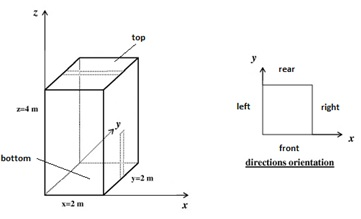
\includegraphics[width=3.0in]{FIGURES/Verification/radiation_verification_case3_enclosure_geometry}
\caption[Geometry for {\ct radiation\_3.in}]{Schematic of the considered geometry.}
\label{fig:rad3_1}
\end{figure}

\begin{figure}[!ht]
\begin{tabular*}{\textwidth}{l@{\extracolsep{\fill}}r}
\includegraphics[width=3.0in]{SCRIPT_FIGURES/Verification/radiation_3_flux_1000_top_gas}
\includegraphics[width=3.0in]{SCRIPT_FIGURES/Verification/radiation_3_flux_1000_side_gas}
\end{tabular*}
\caption[Results of mixture emission case {\ct radiation\_3.in}]{Expected and CFAST calculated target incident heat flux values due to mixture emission for the case {\ct radiation\_3.in}.}
\label{fig:rad3_2}
\end{figure}

\begin{figure}[!ht]
\begin{tabular*}{\textwidth}{l@{\extracolsep{\fill}}r}
\includegraphics[width=3.0in]{SCRIPT_FIGURES/Verification/radiation_3_flux_1000_top_wall}
\includegraphics[width=3.0in]{SCRIPT_FIGURES/Verification/radiation_3_flux_1000_side_wall}
\end{tabular*}
\caption[Results of wall emission case {\ct radiation\_3.in}]{Expected and CFAST calculated target incident heat flux values due to wall emission for the case {\ct radiation\_3.in}.}
\label{fig:rad3_3}
\end{figure}

\subsection{Total Emissivity and Hemispherical Absorptivitiy}
\label{radiation_4and5}

Consider the identical case being described in Section~\ref{radiation_3}. For black surfaces, the total emissivity of the gas medium, radiating to surface $A_{\rm i}$, can be simplified to the following form \cite{Yuen:2014}
\begin{equation}
\mathrm{\epsilon_g \brackets{T_g, T_g}} = \frac{Q_{\rm i}}{A_{\rm i} \sigma T_{\rm g}^4} \quad  ; \quad Q_{\rm i} = \left[ A_{\rm i} -  \sum_{j \neq i} S_{\rm i}S_{\rm j}\brackets{T_g, T_g} \right] \sigma T_{\rm g}^4
\end{equation}
where $Q_{\rm i}$ is the radiative heat transfer to the surface due to the emission from the hot medium from all surrounding surfaces in the direction of surface $A_{\rm i}$. With identical emitting temperature for all surfaces, the hemispherical absorptivity is given to be
\begin{equation}
\mathrm{\alpha_{\rm g}\brackets{T_{\rm w}, T_g}} = \frac{1}{A_{\rm i}} \sum_{j \neq i} \left[ A_{\rm i}F_{\rm i-j} - S_{\rm i}S_{\rm j}\brackets{T_{\rm w,j}, T_{\rm g}} \right]
\end{equation}
The total emissivity and the hemisperical absorptivity of the gas medium for targets on the top surface calculated by CFAST are compared with the benchmark results reported by \cite{Tam:2017}. Two emitting temperatures $T_{\rm w}$ are considered. Results for $T_{\rm w}$ = 226.85 $^\circ$C case and $T_{\rm w}$ = 1226.85 $^\circ$C case are presented in Figure~\ref{fig:rad4_1}.

\begin{figure}[!ht]
\begin{tabular*}{\textwidth}{l@{\extracolsep{\fill}}r}
\includegraphics[width=3.0in]{SCRIPT_FIGURES/Verification/radiation_4_emissivity_500_top_gas}
\includegraphics[width=3.0in]{SCRIPT_FIGURES/Verification/radiation_4_absorptivity_500_top_gas} \\
\includegraphics[width=3.0in]{SCRIPT_FIGURES/Verification/radiation_5_emissivity_1500_top_gas}
\includegraphics[width=3.0in]{SCRIPT_FIGURES/Verification/radiation_5_absorptivity_1500_top_gas}
\end{tabular*}
\caption[Results of $T_w$ = 1226.85 $^\circ$C case {\ct radiation\_5.in}]{Expected and CFAST total emissivity and hemispherical absorptivity of the gas medium to the targets located at top surface for the case {\ct radiation\_5.in}.}
\label{fig:rad4_1}
\end{figure}


\section{Sprinklers}
\label{sprinklers}

\subsection{Utilizing a Sprinkler to Detect and Suppress a Fire}
\label{sprinkler_1}

A constant 10~kW natural gas (methane) fire burns in the center of a 4~m by 4~m by 4~m compartment. The compartment is sealed and a sprinkler is located at the center of the ceiling, with an activation temperature of 40~$^\circ$C and a spray density of 0.07~mm/s. The sprinkler link temperature can be calculated by integrating the following equation \cite{Schifiliti:2002}:
\begin{equation}
\frac{{\rm d} \TL}{{\rm d} t} = \frac{\sqrt{v}}{\rm RTI} \brackets{\Tg - \TL}
\end{equation}
where $\TL$ and $\Tg$ are the link and gas temperatures, $v$ is the gas speed, and RTI (Response Time Index) is a measure of the sensor's thermal inertia. After the sprinkler link temperature reaches the activation temperature, $t > t_{\rm act}$, the sprinkler will begin to suppress the fire by diminishing its heat release rate at the exponential rate described by \cite{Evans:1993}:
\begin{equation}
\dQ(t) = \dQ(t_{\rm act}) \; {\rm e}^{-(t-t_{\rm act}) /\tau}   \quad ; \quad \tau = 3 \, u_{\rm w}^{-1.8}
\end{equation}
where $u_{\rm w}$ is the water spray density, expressed in units of mm/s. Figure~\ref{sprinkler1} shows the sprinkler link temperature rising as the fire burns in the compartment and the heat release rate decreasing exponentially once the sprinkler has been activated.

\begin{figure}[!ht]
\begin{tabular*}{\textwidth}{l@{\extracolsep{\fill}}r}
\includegraphics[width=3.0in]{SCRIPT_FIGURES/Verification/sprinkler_1_link_temp} &
\includegraphics[width=3.0in]{SCRIPT_FIGURES/Verification/sprinkler_1_HRR}
\end{tabular*}
\caption[Results of the test case {\ct sprinkler\_1.in}]{Expected and CFAST calculated values for the sprinkler link temperature and the heat release rate of the fire for the case {\ct sprinkler\_1.in}.}
\label{sprinkler1}
\end{figure}

\section{Fire Ignition}

Two small fires are located in a single compartment some distance away from a larger initiating fire burning in the center of the compartment. The two smaller fires are set to ignite at an incident heat flux of 6~kW/m$^2$ and 200~\degc, respectively. Figures~\ref{fireigntion1} and \ref{fireignition2} show the heat release rate, incident heat flux, and surface temperature for the two fires overlayed with the calculated ignition time.

\begin{figure}[!ht]
\begin{tabular*}{\textwidth}{l@{\extracolsep{\fill}}r}
\includegraphics[width=3.0in]{SCRIPT_FIGURES/Verification/fire_ignition_HRR_1} &
\includegraphics[width=3.0in]{SCRIPT_FIGURES/Verification/fire_ignition_flux_1}
\end{tabular*}
\caption[Results of the test case {\ct Ignition\_Test.in}]{Heat release rate of the fire and incident heat flux to the fire location for the case {\ct Ignition\_Test.in}.}
\label{fireigntion1}
\end{figure}

\begin{figure}[!ht]
\begin{tabular*}{\textwidth}{l@{\extracolsep{\fill}}r}
\includegraphics[width=3.0in]{SCRIPT_FIGURES/Verification/fire_ignition_HRR_2} &
\includegraphics[width=3.0in]{SCRIPT_FIGURES/Verification/fire_ignition_temp_2}
\end{tabular*}
\caption[Results of the test case {\ct Ignition\_Test.in}]{Heat release rate of the fire and surface temperature at the fire location for the case {\ct Ignition\_Test.in}.}
\label{fireignition2}
\end{figure}


\section{Tenability}

\subsection{Gas Tenability}

For the same scenario as the example in section \ref{methane_flame}, gas tenability can be calculated.  A steady-state concentration of 0.0223~\% by volume of CO$_2$, and 0.00137~\% by volume of CO is reached. A 1 s increment of asphyxiant gas FED can by calculated by

\begin{eqnarray}
    \nu_{\rm CO_2} &=& e^{\varphi_{\rm CO_2} \, / \, 5} = e^{0.0223 \, / \, 5} \approx 1 \\[.1in]
    \Delta \chi_{\FED} &=&  \frac{\varphi_{\CO} \cdot \nu_{\COTWO}}{35 000} \, \Delta t =  \frac{13.7 \cdot 1}{35 000} \frac{1}{60} = 0.0000066
\end{eqnarray}
for a 1 s increment. The following figure compares the calculated FED to its expected value.

\begin{figure}[ht]
\centering
\includegraphics[width=3.0in]{SCRIPT_FIGURES/Verification/gas_tenability}
\caption[Results of the test case {\ct gas\_tenability\.in}]{Expected and CFAST calculated values for fractional effective dose due to asphyxiant gases in a one room test case {\ct gas\_tenability.in}.}
\label{fig_gas_tenability}
\end{figure}

\subsection{Heat Tenability}

A compartment is maintained at a constant 100 \degc and a target is placed in the center of the compartment. Heat flux to the target is less than 2.5 kW/m$^2$.  Heat tenability can be calculated by

\be
    \Delta \chi_{\FED} = \frac{1}{4.1 \times 10^8 \, T^{-3.61}} \, \Delta t = 0.00068
\ee
for a 1 s increment. The following figure compares the calculated FED to its expected value.

\begin{figure}[ht]
\centering
\includegraphics[width=3.0in]{SCRIPT_FIGURES/Verification/heat_tenability}
\caption[Results of the test case {\ct heat\_tenability\.in}]{Expected and CFAST calculated values for fractional effective dose due to convected heat in a one room test case {\ct heat\_tenability.in}.}
\label{fig_heat_tenability}
\end{figure}



\section{Summary of Verification Results}

The tests included in this chapter test the energy and mass balance equations in CFAST and various heat transfer (through walls, targets, and fire detectors/sprinklers) and mass transfer (flow through vents) calculations included in the model with comparisons to analytical calculations. These comparisons are an integral part of a process known as regression testing, which aims to evaluate the accuracy of outputs predicted by a numerical software package. The results from this chapter can be compared to another version of CFAST as a way of measuring the quality of results between versions.  These results also help determine the impact of code additions and modifications on the overall accuracy of CFAST and can help identify errors in the CFAST source code. Appendix \ref{info:verification_statistics} presents the results of the verification tests for the current version of CFAST.



\chapter{Description of Validation Experiments}

\label{Experiment_Chapter}

This chapter contains a brief description of the experiments that were used for model validation. Only enough detail is included here to provide a general understanding of the model simulations. Anyone wishing to use the experimental measurements for validation ought to consult the cited test reports or other publications for a comprehensive description.

Much of the content follows the FDS Validation Guide \cite{FDS_Validation_Guide_6} and the verification and validation guide for nuclear power plants developed by the US NRC \cite{NRCNUREG1824}. This study focused on the predicted results of the CFAST fire model and did not include an assessment of the user interface for the model.  However, all input files used for the simulations were prepared using the CFAST graphical user interface (GUI) and reviewed for correctness prior to the simulations.  The comparisons between the experiments and model predictions were characterized as open calculations, i.e., the modelers were given detailed descriptions of the test conditions, test geometry, and fire source, but did not modify model inputs from these given conditions to improve model predictions.  As such, the comparisons in this report provide an assessment of the predictive capability of the model, but not an assessment of the ability of different modelers to develop appropriate model inputs.


\newpage

\section{ATF Corridors Experiments}

A series of eighteen experiments were conducted in a two-story structure with long hallways and a connecting stairway
in the large burn room of the ATF Fire Research Laboratory in Ammendale, Maryland, in 2008~\cite{Sheppard:Corridors}.
The test enclosure consisted of two 17.0~m long hallways connected by a
stairway consisting of two staircases and an intermediary landing.
There was a door at the opposite end of the first floor hallway, which was closed during all tests.
The end of the second floor hallway was open with a soffit near the ceiling.

The walls and ceilings of the test structure were constructed of 1.2~cm gypsum wallboard.
The flooring throughout the structure, including the stairwell landing floor, consisted of one layer of 1.3~cm thick cement board on one
layer of 1.9~cm thick plywood supported by wood joists. The first set of stairs, which had eight risers, led from the first floor up to the landing area.
The second set of stairs, which had nine risers, led from the landing area up to the second floor.
The stairs were constructed of 2.5~cm thick clear pine lumber. The two set of stairs were separated by an approximately 0.42~m wide gap in the middle of the stairwell.
This gap was separated from the stairs by a 0.91~m tall barrier constructed of a single piece of gypsum board.
The flue space was open to the first floor.  The flue space was separated from the second floor by a 0.9~m tall barrier constructed of gypsum board.
There was a metal exterior type door at the end of the first floor near the burner.  The door was closed during all experiments.

The fire source was a natural gas diffusion flame burner.  The burner surface was horizontal, square and 0.45~m on each side, its surface was 0.37~m above the floor, and it was filled with gravel.
The burner was located near the end of the first floor away from the stairs. A diagram of the test structure is displayed in Figure~\ref{ATF Drawing}.


\begin{figure}[h]
\begin{center}
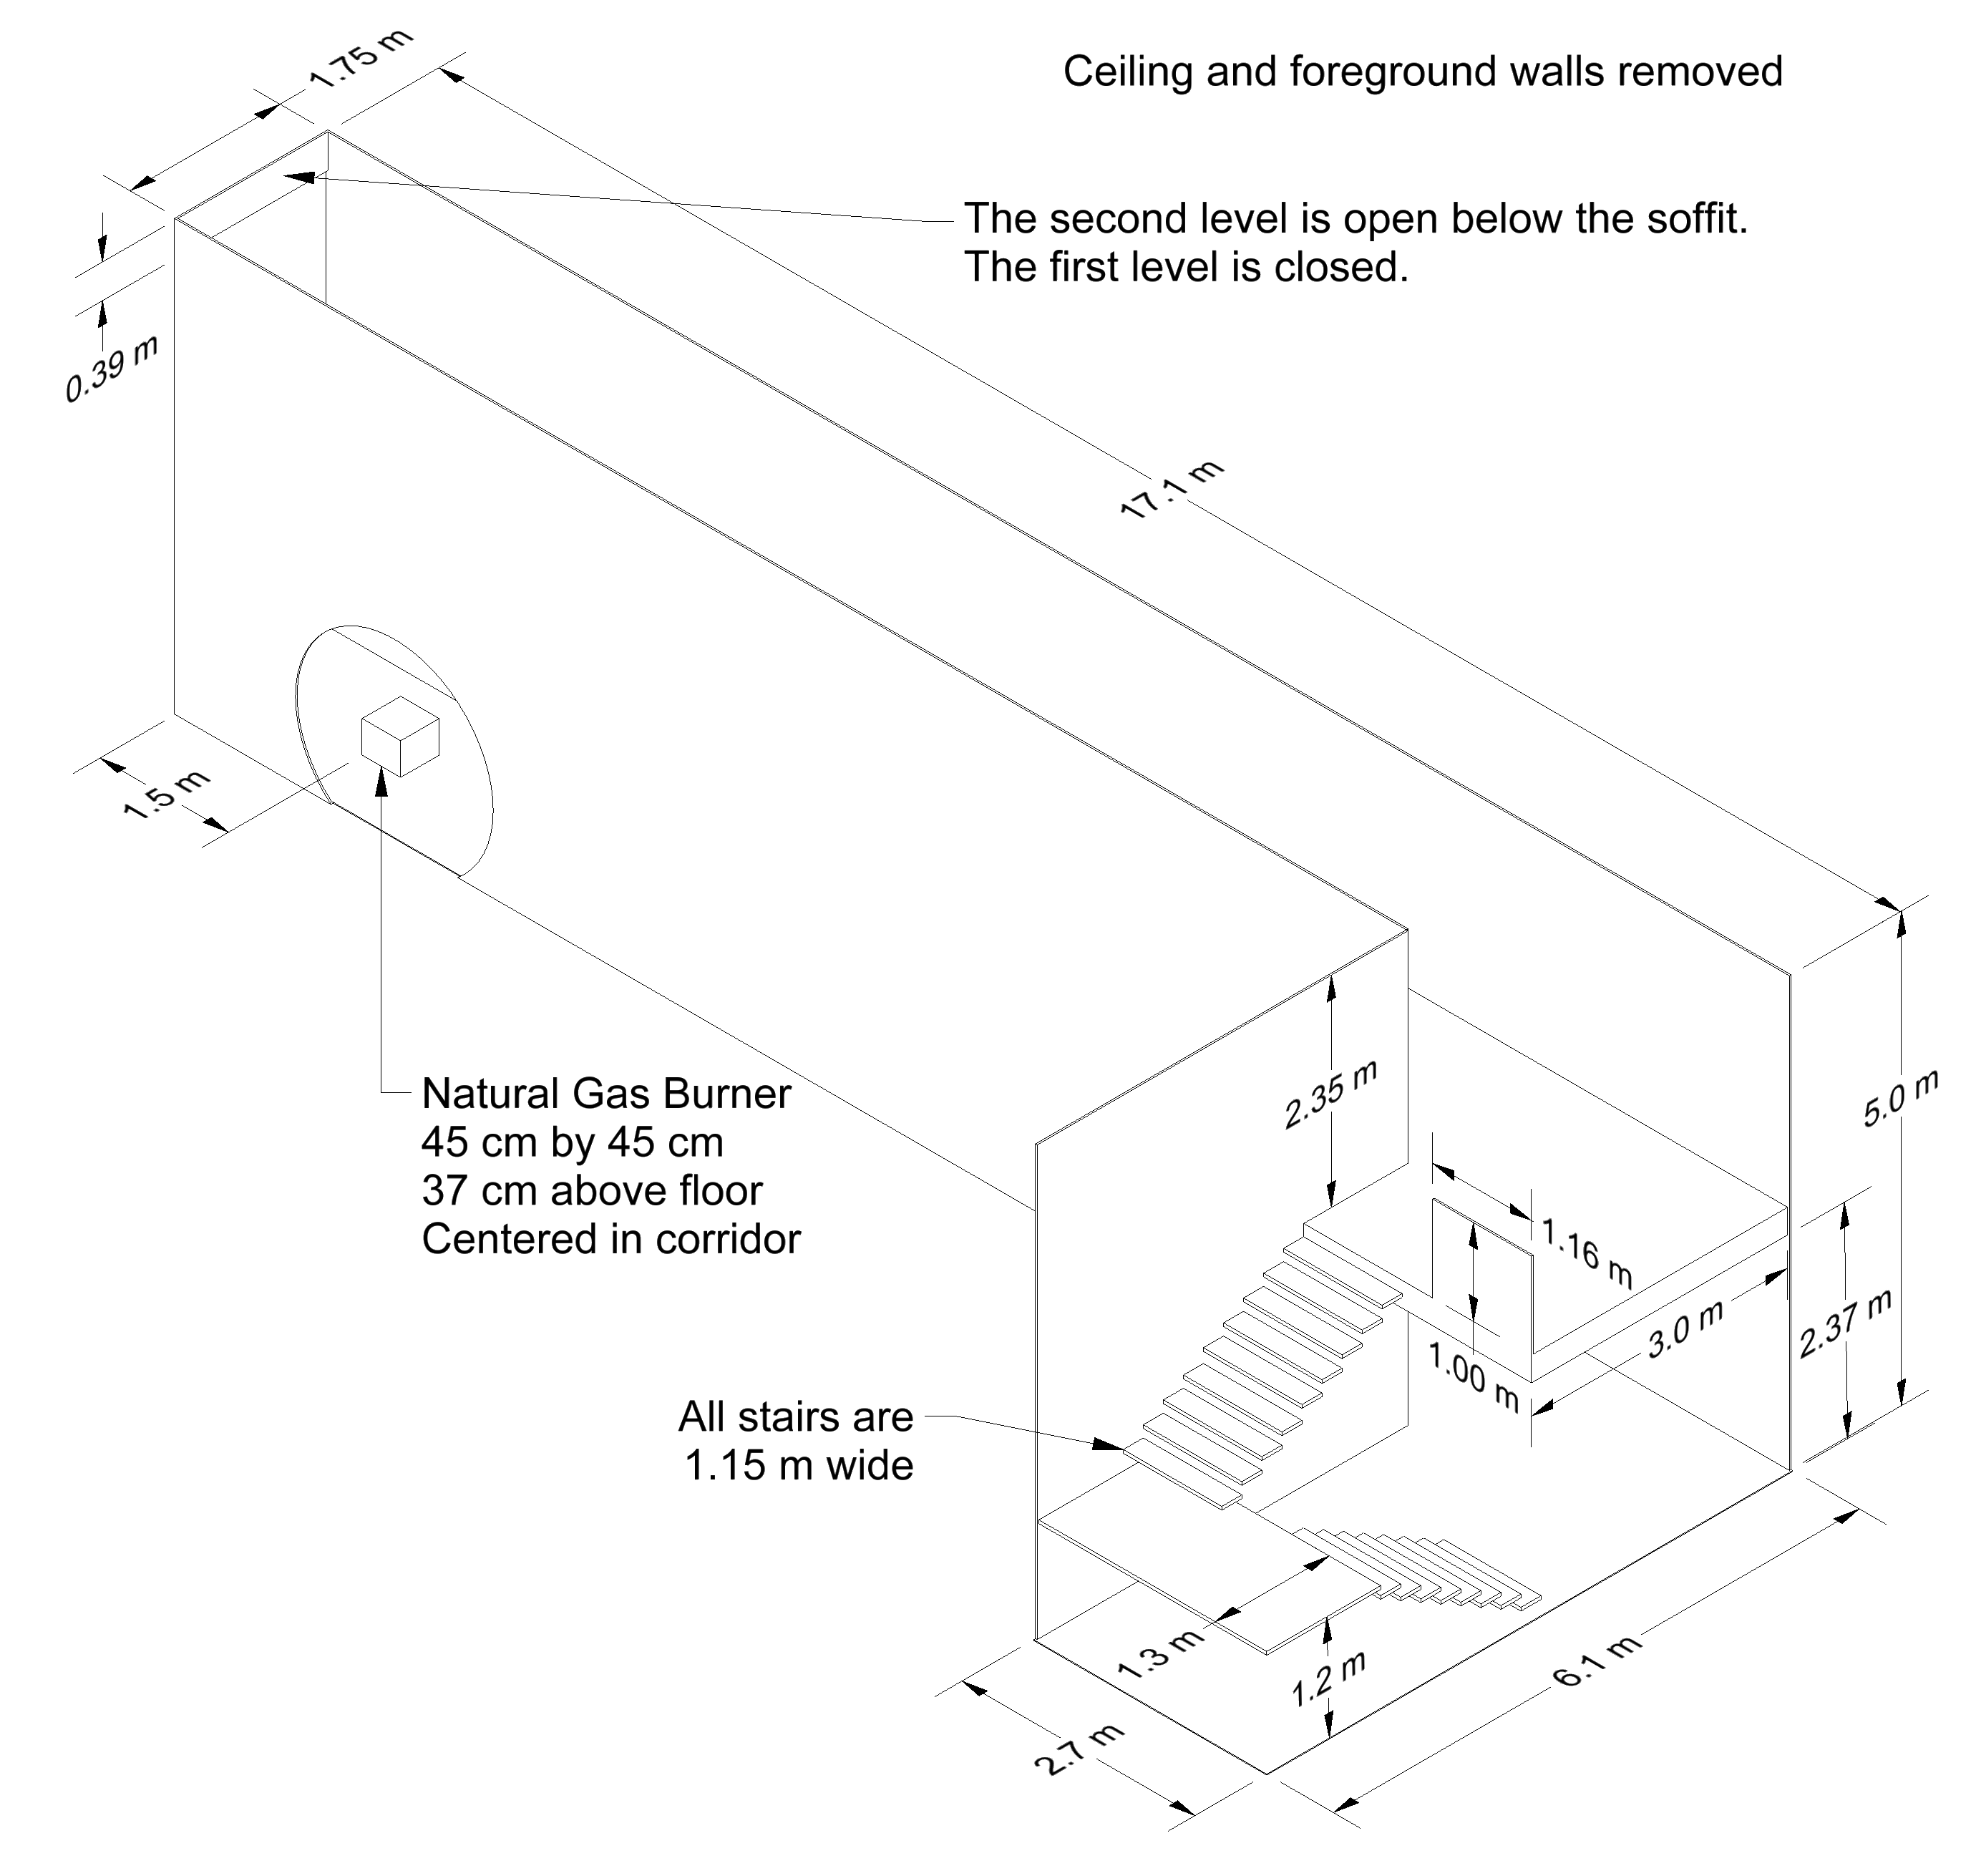
\includegraphics[width=6.5in]{FIGURES/ATF_Corridors/ATF_Corridors_Drawing}
\end{center}
\caption{Geometry of the ATF Corridors Experiments.}
\label{ATF Drawing}
\end{figure}

\FloatBarrier


\section{Fleury Heat Flux Measurements}

Rob Fleury, a masters degree student at the University of Canterbury in Christchurch, New Zealand, measured the heat flux from a variety of propane fires~\cite{Fleury:Masters}.
The objective of the work was to evaluate a variety of empirical heat flux calculation methods. For the measurements, heat flux gauges were mounted on moveable dollies that
were placed in front of, and to the side of, burners with dimensions of 0.3~m by 0.3~m (1:1 burner), 0.6~m by 0.3~m (2:1 burner), and 0.9~m by 0.3~m (3:1 burner). The heat release
rates were set to 100~kW, 150~kW, 200~kW, 250~kW, and 300~kW. The gauges were mounted at heights of 0~m, 0.5~m, 1.0~m, and 1.5~m relative to the top edge of the burner.

\section{FM Four Room Including Corridor Test Series}

This data set describes a series of tests conducted in a multiple room configuration with more complex gas burner fires than the previous data set.  This study \cite{Heskestad:1986} was included because, in many ways, it is similar to the smoke movement study performed at NBS \cite{Peacock:1988}, and permits comparisons between two different laboratories. In addition, it expands upon that data set by providing larger a time-varying gas burner fires in a room-corridor configuration. Fire size was about up to 1 MW with a total volume of 200 m$^3$.

This study was performed to collect data allowing for variations in fire source, ventilation, and geometry in a multi-compartment structure, especially for situations with closed doors. This test program was carried out at Factory Mutual Research Corporation (FMRC) in West Glocester, RI, in which 60 fire experiments were conducted in a multiple-room enclosure to furnish validation data for theoretical fire models.

Figure \ref{fig:FMSummary} shows a diagram of the basic facility with indications of instrumentation location. The facility was built on the floor of FMRC's fire test building, using part of the 67 m by 76 m test building where the ceiling height is 18.3 m. The layout in figure 25 shows a burn room and two target rooms connected to a corridor. The corridor was 2.43 m wide x 18.89 m long x 2.43 m high. The burn room measured 3.63 m deep x 3.64 m wide x 2.45 m high; a sealable window opening, measuring 0.85 m square, was centered on the rear wall, 0.34 m down from the top, and a door, measuring 0.92 m by 2.05 m high, was centered on the front wall (opening to the corridor). For closed window experiments, the wood-framed calcium silicate board window cover was pressed against a bead of caulking around the steel window frame and held by drop bars positioned into slots on the outside wall.

\begin{figure}[h]
\begin{center}
\begin{tabular}{cc}
\includegraphics[width=6.0in]{FIGURES/FM_NBS/FMSummary}\\
\end{tabular}
\end{center}
\caption{Overview of the {F}actory {M}utual Four Room test series.}
 \label{fig:FMSummary}
\end{figure}

Room 3, located opposite the burn room, measured 3.65 m deep x 3.64 m wide x 2.45 m high; a door, measuring 0.88 m by 2.02 m high, was centered on the front wall (opening to the corridor). Room 4, located at the opposite end of the corridor, measured 3.65 m deep x 3.65 m wide x 2.43 m high and had a 0.88 m by 2.02 m high door centered on the front wall (opening to the corridor); an observation alcove, measuring 1.28 m by 0.86 m by 1.99 m high, was located in the front corner of room 4. Each room was equipped with a 102~mm inside diameter vent tube with a 61 mm inside diameter orifice meter and thermocouple, with option of exhaust fan (tube centered 0.27 m from the floor and 0.17 m from the closest parallel wall). An inlet vent (0.29 m$^2$) used with exhaust fans was centered 0.43 m above the floor at the end of the corridor between the burn room and room 3. When not in use, the inlet vent was sealed with a gypsum board cover taped in place.

The target room doors were commercial fire doors (wood-faced composite doors with calcium silicate cores, 14 h rated) mounted on 16 gage steel frames. The burn room door was fabricated from 12.7 mm calcium silicate, mounted in a steel frame lined with calcium silicate. Details of the doors and the spacings (cracks) are given in the original reference \cite{Heskestad:1986}.

Gypsum wallboard, 12.7 mm thick, on wood studs was used throughout the experimental facility. In addition, the walls and ceiling of the burn room were overlaid with calcium silicate, also 12.7 mm thick, to harden against repeated fire exposure. The existing concrete floor of the test building was used.

Two types of fire sources were used: 1) steady propylene fires at 56 kW on a 0.30 m diameter sand burner and 522 kW on a 0.91 m diameter burner and 2) propylene fires on the 0.91 m diameter burner programmed under computer control to grow with the square of time, exceeding 1 MW in 1, 2, 4, or 8 min.

The 0.91 m diameter, 0.58 in high propylene burner was used for most of the tests. Its design consisted of a 12 gage steel container with a gas distributor near the bottom, filled with gravel to a 67 percent height, where there was wire mesh screen, and coarse sand to the full height of the burner. The 0.30 m diameter burner was a scaled-down version of similar design.

\section{FM / SNL Test Series}

The Factory Mutual and Sandia National Laboratories (FM/SNL) test series consists of 25 compartment fire experiments conducted in 1985 for the U.S.~Nuclear Regulatory Commission (NRC) by Factory Mutual Research Corporation (FMRC), under the direction of Sandia National Laboratories (SNL)~\cite{Nowlen:NUREG4681,Nowlen:NUREG4527}. The primary purpose of these experiments was to provide data with which to validate computer models for various types of compartments typical of nuclear power plants. The experiments were conducted in an enclosure measuring approximately 18~m long by 12~m wide by 6~m high, constructed at the FMRC fire test facility in Rhode Island. A drawing is included in Fig.~\ref{FM_SNL_Drawing}. All of the experiments included forced ventilation to simulate typical power plant conditions. Six of the experiments were conducted with a full-scale control room mock-up in place. Parameters varied during the experiments included fire intensity, enclosure ventilation rate, and fire location. Only data from nineteen experiments (Tests 1-17, 21, and 22) is used in the current study. In these experiments, the fires were fueled by a propylene gas burner, and heptane and methanol liquid pools. In the experiments not selected, the heat release was not reported and could not be estimated with confidence. Table~\ref{FM_SNL_Matrix} lists the test parameters.

The following information was provided by the test director, Steve Nowlen of Sandia National Laboratory. In particular, Tests 4, 5, and 21 were given extra attention.
\begin{description}
\item[Heat Release Rate:] The HRR was determined using oxygen consumption calorimetry in the exhaust stack with a correction applied for the carbon dioxide in the upper layer of the compartment. The uncertainty of the fuel mass flow was not documented. Several tests selected for this study had the same target peak heat release rate of 516~kW following a 4~min ``t-squared'' growth profile. The test report contains time histories of the measured HRR, for which the average, sustained HRR following the ramp up for Tests 4, 5, and 21 have been estimated as 510~kW, 480~kW, and 470~kW, respectively. Once reached, the peak HRR was maintained essentially constant during a steady-burn period of 6~min in Tests~4 and 5, and 16~min in Test~21. Note that in Test 21, Nowlen reports a ``significant'' loss of effluent from the exhaust hood that could lead to an under-estimate of the HRR towards the end of the experiment.
\item[Radiative Fraction:] The radiative fraction was not measured during the experiment, but in this study it is assumed to equal 0.35, which is typical for a smoky hydrocarbons. It was further assumed that the radiative fraction was about the same in Test~21 as the other tests, as fuel burning must have occurred outside of the electrical cabinet in which the burner was placed.
\item[Measurements:] Four types of measurements were conducted during the FM/SNL test series that are used in the current model evaluation study, including the HGL temperature and depth, and the ceiling jet and plume temperatures. Aspirated thermocouples (TCs) were used to make all of the temperature measurements. Generally, aspirated TC measurements are preferable to bare-bead TC measurements, as systematic radiative exchange measurement error is reduced.
\item[HGL Depth and Temperature:] Data from all of the vertical TC trees were used when reducing the HGL height and temperature. For the majority of the tests, Sectors 1, 2, and 3 were used, all weighted evenly. For Tests 21 and 22, Sectors 1 and 3 were used, evenly weighted. Sector 2 was partially within the fire plume.
\end{description}



\begin{table}[h!]
\caption[Summary of FM/SNL Experiments]{Summary of FM/SNL Experiments. ACH stands for Air Changes per Hour.}
\begin{center}
\begin{tabular}{|c|c|c|c|c|c|}
\hline
Test    &  Fuel             & Nominal Peak  & Fire          & Ventilation       & Room                   \\
No.     &  Type             & HRR (kW)      & Position      & Rate (ACH)        & Configuration          \\ \hline \hline
1       & Propylene Burner  &     516       & Center        & 10                & Empty                  \\ \hline
2       & Propylene Burner  &     516       & Center        & 10                & Empty                  \\ \hline
3       & Propylene Burner  &    2000       & Center        & 10                & Empty                  \\ \hline
4       & Propylene Burner  &     516       & Center        & 1                 & Empty                  \\ \hline
5       & Propylene Burner  &     516       & Center        & 10                & Empty                  \\ \hline
6       & Heptane Pool      &     500       & Wall          & 1                 & Empty                  \\ \hline
7       & Propylene Burner  &     516       & Center        & 1                 & Empty                  \\ \hline
8       & Propylene Burner  &    1000       & Center        & 1                 & Empty                  \\ \hline
9       & Propylene Burner  &    1000       & Center        & 8                 & Empty                  \\ \hline
10      & Heptane Pool      &    1000       & Wall          & 4.4               & Empty                  \\ \hline
11      & Methanol Pool     &     500       & Wall          & 4.4               & Empty                  \\ \hline
12      & Heptane Pool      &    2000       & Wall          & 4.4               & Empty                  \\ \hline
13      & Heptane Pool      &    2000       & Wall          & 8                 & Empty                  \\ \hline
14      & Methanol Pool     &     500       & Wall          & 1                 & Empty                  \\ \hline
15      & Heptane Pool      &    1000       & Wall          & 1                 & Empty                  \\ \hline
16      & Heptane Pool      &     500       & Corner        & 1                 & Empty                  \\ \hline
17      & Heptane Pool      &     500       & Corner        & 10                & Empty                  \\ \hline
21      & Propylene Burner  &     500       & Cabinet       & 1                 & Furnished              \\ \hline
22      & Propylene Burner  &    1000       & Cabinet       & 1                 & Furnished              \\ \hline
\end{tabular}
\end{center}
\label{FM_SNL_Matrix}
\end{table}



\begin{figure}[p]
\includegraphics[width=\textwidth]{FIGURES/FM_SNL/FM_SNL_Drawing}
\caption[Geometry of the FM/SNL Experiments]{Geometry of the FM/SNL Experiments.}
\label{FM_SNL_Drawing}
\end{figure}

\FloatBarrier


\section{iBMB Compartment Tests}

A series of small compartment kerosene pool fire experiments, conducted at the Institut f\"ur Baustoffe, Massivbau und Brandschutz (iBMB) of Braunschweig University of Technology in Germany in 2004 ~\cite{Klein-Helbetaling:2005}. These experiments involved relatively large fires in a relatively small (3.6 m by 3.6 m by 5.7 m) concrete enclosure. Figure~\ref{fig:iBMB_Pool_Detailed} shows plan, side and perspective schematic drawings of the experimental arrangement, including the location of the fuel pan, which was located at the center of the compartment.

\begin{figure}[p]
\begin{center}
\includegraphics[width=6.5in]{FIGURES/iBMB/iBMB_Pool}\\
\end{center}
\caption{Detailed plan, side, and perspective schematic drawings of the iBMB pool fire experimental arrangement.}
 \label{fig:iBMB_Pool_Detailed}
\end{figure}

A second series of fire experiments in 2004, conducted under the International Collaborative Fire Model Project (ICFMP) involved realistically routed cable trays inside the same concrete enclosure at iBMB~\cite{Riese:2004}. The compartment was configured slightly differently with a ceiling height of 5.6 m. A schematic diagram from plan, side, and perspective views of the experimental arrangement is shown in figure \ref{fig:iBMB_Cable_Detailed}.

\begin{figure}[p]
\begin{center}
\includegraphics[width=6.5in]{FIGURES/iBMB/iBMB_Cable}\\
\end{center}
\caption{Detailed plan, side, and perspective schematic drawings of the iBMB cable fire experimental arrangement.}
 \label{fig:iBMB_Cable_Detailed}
\end{figure}

\FloatBarrier

\section{LLNL Enclosure Tests}

Sixty-four enclosure fire tests were conducted by Lawrence Livermore National Laboratory (LLNL) in 1986 to study the effects of ventilation on enclosure fires~\cite{Foote:LLNL1986}. The test
enclosure was 6~m long, 4~m wide, and 4.5~m high. It contained a methane rock burner which was placed in the center of the space. For most of the tests the burner was placed on the
floor. The fires varied in size from 50~kW to 400~kW. The burner was 0.57~m in diameter and 0.23~m height.

The door (2.06 m high by 0.76 m wide) was closed and sealed for most tests, and air was pulled through the space at rates varying from 100 to 500~g/s. In some tests the enclosure included a plenum space, where
make-up air could be injected from above or below. The test matrix is listed in Table~\ref{LLNL_Matrix}.

\begin{table}[p]
\caption[Summary of LLNL Enclosure Experiments]{Summary of LLNL Enclosure Experiments.}
\begin{center}
\begin{tabular}{|c|c|c|c|c|c||c|c|c|c|c|c|}
\hline
Test & Room    & $h_0$ &  $\dot{Q}$ & $\dot{m}$ & $T_\infty$  &   Test & Room    & $h_0$ &  $\dot{Q}$ & $\dot{m}$ & $T_\infty$  \\
No.  & Config. & m     &  kW        & g/s       & $^\circ$C   &   No.  & Config. & m     &  kW        & g/s       & $^\circ$C   \\ \hline \hline
1    & TL      & 0     & 200        & 0         & 23          &   33   & PH      & 0     & 100        & 200       & 23          \\ \hline
2    & TL      & 0     & 200        & 0         & 27          &   34   & PH      & 0     & 100        & 300       & 34          \\ \hline
3    & TL      & 0     & 400        & 0         & 27          &   35   & PH      & 0     & 100        & 400       & 22          \\ \hline
4    & TL      & 0     & 300        & 0         & 24          &   36   & PH      & 0     & 100        & 500       & 29          \\ \hline
5    & TL      & 0     & 50         & 0         & 28          &   37   & PH      & 0     & 200        & 100       & 20          \\ \hline
6    & TL      & 0     & 100        & 0         & 29          &   38   & PH      & 0     & 200        & 300       & 29          \\ \hline
7    & TL      & 0     & 100        & 0         & 35          &   39   & PH      & 0     & 250        & 100       & 18          \\ \hline
8    & TL      & 0     & 200        & 0         & 35          &   40   & PH      & 0     & 200        & 400       & 28          \\ \hline
9    & TL      & 0     & 200        & 500       & 33          &   41   & PH      & 0     & 150        & 100       & 20          \\ \hline
10   & TL      & 0     & 200        & 100       & 28          &   42   & PHE     & 2     & 200        & 180       & 30          \\ \hline
11   & TL      & 0     & 200        & 200       & 18          &   43   & PHE     & 2     & 200        & 0         & 32          \\ \hline
12   & TL      & 0     & 200        & 300       & 21          &   44   & PHE     & 1     & 200        & 180       & 19          \\ \hline
13   & TL      & 0     & 200        & 400       & 28          &   45   & PHE     & 1     & 200        & 0         & 30          \\ \hline
14   & TL      & 0     & 200        & 400       & 28          &   46   & PHE     & 0.6   & 200        & 180       & 19          \\ \hline
15   & TL      & 0     & 100        & 300       & 24          &   47   & PHE     & 0.6   & 200        & 0         & 19          \\ \hline
16   & TL      & 0     & 200        & 300       & 21          &   48   & PHE     & 0.3   & 200        & 0         & 21          \\ \hline
17   & PL      & 0     & 200        & 500       & 26          &   49   & PHE     & 0.3   & 200        & 180       & 26          \\ \hline
18   & PL      & 0     & 200        & 400       & 21          &   50   & PHE     & 1     & 200        & 180       & 21          \\ \hline
19   & PL      & 0     & 200        & 300       & 18          &   51   & PNE     & 1     & 200        & NAT       & 33          \\ \hline
20   & PL      & 0     & 200        & 200       & 16          &   52   & PN      & 0     & 200        & NAT       & 23          \\ \hline
21   & PL      & 0     & 200        & 100       & 23          &   53   & PHGS    & 0     & 200        & 185       & 33          \\ \hline
22   & PH      & 0     & 200        & 190       & 30          &   54   & PHGS    & 0     & 200        & 215       & 21          \\ \hline
23   & PH      & 0     & 200        & 215       & 28          &   55   & PN      & 0     & 100        & NAT       & 31          \\ \hline
24   & PH      & 0     & 200        & 205       & 26          &   56   & PHGW    & 0     & 200        & 190       & 20          \\ \hline
25   & PH      & 0     & 200        & 205       & 25          &   57   & PHGW    & 0     & 200        & 215       & 29          \\ \hline
26   & PH      & 0     & 200        & 500       & 24          &   58   & PHX     & 0     & 200        & 190       & 18          \\ \hline
27   & PH      & 0     & 200        & 100       & 23          &   59   & PHXE    & 1     & 200        & 190       & 24          \\ \hline
28   & PH      & 0     & 150        & 150       & 31          &   60   & PN      & 0     & 400        & NAT       & 22          \\ \hline
29   & PH      & 0     & 250        & 250       & 28          &   61   & TN      & 0     & 200        & NAT       & 31          \\ \hline
30   & PH      & 0     & 250        & 300       & 34          &   62   & TN      & 0     & 400        & NAT       & 22          \\ \hline
31   & PH      & 0     & 250        & 500       & 36          &   63   & TN      & 0     & 50         & NAT       & 28          \\ \hline
32   & PH      & 0     & 100        & 100       & 33          &   64   & TN      & 0     & 100        & NAT       & 17          \\ \hline
\end{tabular}
\end{center}
\begin{tabbing}
\hspace{0.7in} \= T \hspace{0.2in}  \= full compartment     \hspace{0.8in} \= N \hspace{0.2in} \= natural ventilation (door open) \\
               \> P                 \> plenum configuration                \> X                \> 3 ft extension on inlet opening \\
               \> L                 \> low inlet duct                      \> GS               \> grate on inlet, north/south configuration \\
               \> H                 \> high inlet duct                     \> GW               \> grate on inlet, east/west configuration \\
               \> E                 \> elevated fire, $h_0$
\end{tabbing}
\label{LLNL_Matrix}
\end{table}


\begin{figure}
\begin{center}
\includegraphics[width=6.5in]{FIGURES/LLNL_Enclosure/LLNL_Enclosure_Drawing}
\end{center}
\caption[Geometry of the LLNL Enclosure Experiments]{Geometry of the LLNL Enclosure Experiments.}
\label{LLNL_Enclosure_Drawing}
\end{figure}

\FloatBarrier

\section{NBS Single Room Tests with Furniture}

These data describe a series of room fire tests using upholstered furniture items in a room of fixed size but with varying opening sizes and shapes \cite{Valid:Babrauskas_Flashover} conducted by the National Bureau of Standards (NBS, former name of NIST). It was selected for its well characterized and realistic fuel sources in a simple single-room geometry. In addition, the wide variation in opening size should provide challenges for current zone fire models. Peak fire size was about 2.9~MW with a total room volume of 21 m$^3$. A series of four single-room fire tests were conducted using upholstered furniture items for comparison with their free burning behavior, previously determined in a furniture calorimeter.  The experiments were conducted in a single room enclosure; ventilation to the room was provided by window openings of  varying sizes. The room was equipped with an instrumented exhaust collection system outside the window opening.

A second similar test series also utilized a single-room fire test with furniture as the fire source \cite{Lee:1985}. It expanded upon the first data set by adding the phenomenon of wall burning. Peak fire size was about 7 MW. The room size was similar to the first test series. Figure \ref{fig:NBSFurniture} illustrates the configuration for the two test series.

\begin{figure}
\begin{center}
\includegraphics[width=5.0in]{FIGURES/NBS/NBSFurniture}\\
\end{center}
\caption[Plan and elevation view schematic of experimental room for NBS single room tests with furniture.]{Plan and elevation view schematic of experimental room for NBS single room tests with furniture. Note dotted lines on burning specimen indicates vertical surface for wall burning experiments.  Specimen and instrumentation placement are approximate.}
 \label{fig:NBSFurniture}
\end{figure}

\begin{figure}
\begin{center}
\includegraphics[width=5.0in]{FIGURES/NBS/NBS_Furniture_Test}\\
\end{center}
\caption[Burning specimen during NBS single room tests with furniture.]{Burning specimen during NBS single room tests with furniture.}
 \label{fig:NBSFurniturePix}
\end{figure}

The test furniture included a 28.3 kg armchair or a similar 40.0 kg love seat for the first test series. Both were of conventional wood frame construction and used polyurethane foam padding, made to minimum California State flammability requirements, and polyolefin fabric. A single piece of test furniture and igniting wastebasket were the only combustibles in the test room.

For the second test series, room furnishings consisted of a 1.37 m wide x 1.91 m long x 0.53 m high double bed, a 2.39 m X 0.89 m high headboard, and 0.51 m wide x 0.41 m deep x 0.63 m high night table. Both headboard and night table were fabricated from 12.7 mm thick plywood. The bedding was comprised of two pillows, two pillow cases, two sheets, and one blanket. The pillows had a polypropylene fabric with a polyester filling. The pillow cases and sheets were polyester-cotton. The blanket was acrylic material. The bedding was left in a "slept in" condition which was duplicated to the degree possible in each test. In all of the tests, the fire was started with match flame ignition of a 0.34 kg (240 mm x 140 mm x 240 mm high) wastebasket, filled with 0.41 kg of trash, positioned adjacent to the bed.

\FloatBarrier

\section{NBS Multi-Compartment Test Series}

The National Bureau of Standards (NBS, which is now called the National Institute of Standards and Technology, NIST) Multi-Room Experiments consisted of 45 fire tests representing 9 different sets of conditions were conducted in a three-room suite (see Figs.~\ref{fig:NBS_100kW_fire} and \ref{fig:NBS_Detailed}). The experiments were conducted in 1985 and are described in detail in Ref.~\cite{Peacock:1988}. The suite consisted of two relatively small rooms, connected via a relatively long corridor. The fire source, a gas burner, was located against the rear wall of one of the small compartments.  Fire tests of 100~kW, 300~kW and 500~kW were conducted. For the current study, only three 100~kW fire experiments have been used, including Test~100A from Set~1, Test~100O from Set~2, and Test~100Z from Set~4. These tests were selected because they had been used in prior validation studies, and because these tests had the steadiest values of measured heat release rate during the steady-burn period.

Following is additional information provided by the test director, Richard Peacock of NIST:
\begin{description}
\item[Heat Release Rate:] In the two tests for which
the door was open, the HRR during the steady-burn period measured via oxygen consumption
calorimetry was 110~kW with an uncertainty of about 15~\%, consistent with the replicate
measurements made during the experimental series and the uncertainty typical of oxygen
consumption calorimetry. It was assumed that the closed door test (Test~100O) had the same HRR as the open
door tests.
\item[Radiative Fraction:] Natural gas was used as the fuel in
Test~100A. In Tests~100O and 100Z, acetylene was added to the natural gas to increase the
smoke yield, and as a consequence, the radiative fraction increased. The radiative fraction of
natural gas has been studied previously, whereas the radiative fraction of the acetylene/natural
gas mixture has not been studied. The radiative fraction for the natural gas fire was assigned a
value of 0.20, whereas a value of 0.30 was assigned for the natural gas/acetylene fires.
\item[Measurements:] Only two types of measurements conducted during the NBS test series were used in the
evaluation considered here, because there was less confidence in the other measurements.
The measurements considered here were the HGL temperature and depth, in which bare bead
TCs were used to make these measurements. Single point measurements of temperature within
the burn room were not used in the evaluation of plume or ceiling jet algorithms. This is because
the geometry was not consistent in either case with the assumptions used in the model algorithms
of plumes or jets. Specifically, the burner was mounted against a wall, and the room width-to-height
ratio was less than that assumed by the various ceiling jet correlations.
\end{description}

\begin{figure}
\begin{center}
\includegraphics[width=2.0in]{FIGURES/NBS/NBS_100kW_fire}  \\
\end{center}
\caption{Photo of a 100 kW fire with the burner located against the rear wall of one of the small compartments in the NBS Multi-Compartment test Series.}
 \label{fig:NBS_100kW_fire}
\end{figure}

\begin{figure}
\begin{center}
\includegraphics[width=6.5in]{FIGURES/NBS/NBS_Drawing}\\
\end{center}
\caption{Plan, side and perspective schematic drawings of the NBS experimental arrangement, including the burner.}
 \label{fig:NBS_Detailed}
\end{figure}

\FloatBarrier

\section{NIST / NRC Compartment Experiments}


These experiments, sponsored by the US NRC and conducted at NIST, consisted of 15 large-scale experiments performed in June 2003. All 15 tests were included in the validation study. The experiments are documented in Ref.~\cite{Hamins:2005}. The fire sizes ranged from 350 kW to 2.2 MW in a compartment with dimensions 21.7~m by 7.1~m by 3.8~m high, designed to represent a compartment in a nuclear power plant containing power and control cables. A photo of the fire seen through the compartment doorway is shown in figure \ref{fig:NISTNRC_1MW_fire}. A diagram of the test structure is displayed in Figure~\ref{fig:NISTNRC_Detailed}.

\begin{figure}
\begin{center}
\includegraphics[width=4.0in]{FIGURES/NIST_NRC/NISTNRC_1MW_fire}\\
\end{center}
\caption{Photograph of a 1 MW heptane fire seen through the open doorway. Photo provided by Anthony Hamins, NIST.}
 \label{fig:NISTNRC_1MW_fire}
\end{figure}

\begin{figure}
\begin{center}
\includegraphics[width=6.5in]{FIGURES/NIST_NRC/NIST_NRC_Drawing}\\
\end{center}
\caption{Plan, side and perspective schematic drawings of the NIST NRC experimental arrangement. The fuel pan and cables B, D, F, and G (dotted lines) are also shown.}
 \label{fig:NISTNRC_Detailed}
\end{figure}

The walls and ceiling were covered with two layers of marinate boards, each layer 0.0125~m thick. The floor
was covered with one layer of gypsum board on top of a layer of plywood. Thermo-physical and optical properties of the marinate
and other materials used in the compartment are given in Ref.~\cite{Hamins:2005}. The room had one door and a mechanical air injection and extraction
system. Ventilation conditions, the fire size, and fire location were varied. Numerous measurements (approximately 350 per test) were made including
gas and surface temperatures, heat fluxes and gas velocities.

Following are some notes provided by Anthony Hamins, who conducted the experiments:
\begin{description}
\item[Natural Ventilation:] The compartment had a 2~m by 2~m door in the middle of the west wall. Some of the tests had a closed door and no mechanical
ventilation (Tests 2, 7, 8, 13, and 17), and in those tests the measured compartment leakage was an important consideration. The test report lists leakage
areas based on measurements performed prior to Tests 1, 2, 7, 8, and 13. For the closed door tests, the leakage area used in the simulations was
based on the last available measurement. The chronological order of the tests differed from the numerical order.
For Test 4, the leakage area measured before Test 2 was used. For Tests 10 and 16, the leakage area
measured before Test 7 was used.
\item[Mechanical Ventilation:] The mechanical ventilation and exhaust was used during Tests 4, 5, 10, and 16, providing about 5 air changes per hour. The
door was closed during Test 4 and open during Tests 5, 10, and 16. The supply duct was positioned on the south wall, about 2~m off the floor. An
exhaust duct of equal area to the supply duct was positioned on the opposite wall at a comparable location. The flow rates through the supply and
exhaust ducts were measured in detail during breaks in the testing, in the absence of a fire. During the tests, the flows were monitored with single
bi-directional probes during the tests themselves.
\item[Heat Release Rate:] A single nozzle was used to spray liquid hydrocarbon fuels onto a 1~m by 2~m fire pan that was about 0.1~m deep. The test plan
originally called for the use of two nozzles to provide the fuel spray. Experimental observation suggested that the fire was less unsteady with the
use of a single nozzle. In addition, it was observed that the actual extent of the liquid pool was well-approximated by a 1~m circle in the
center of the pan. For safety reasons, the fuel flow was terminated when the lower-layer oxygen concentration
dropped to approximately 15~\% by volume.
The fuel used in 14 of the tests was heptane, while toluene was used for one test. The HRR was
determined using oxygen consumption calorimetry. The recommended uncertainty values
were 17~\% for all of the tests.
\item[Radiative Fraction:]  The values of radiative fraction and its uncertainty were reported as
\num{0.44 \pm 0.07} and \num{0.40 \pm 0.09} for heptane and toluene, respectively.
\item[Soot Yield:]  The values of the soot yield and its uncertainty were reported as \SI{0.0149 \pm 0.0033}{kg/kg}
and \SI{0.195 \pm 0.052}{kg/kg} for heptane and toluene, respectively.
\end{description}

\FloatBarrier


\section{NIST/NRC Corner, Wall, and Cabinet Experiments}

In the summer of 2017, experiments were conducted in a large compartment in the NIST large fire laboratory on behalf of the U.S. Nuclear Regulatory Commission. There were two sets of experiments. In the first set, conducted in July, 2017, a natural gas burner was positioned either in a corner or against a wall, and gradually moved outward. In the second set of experiments, conducted in September, 2017, a natural gas burner was placed inside one of two steel cabinets meant to represent typical industrial-scale electrical enclosures.

The compartment for all experiments was 11~m long, 7~m wide, and 3.8~m high. The long dimension of the compartment ran east-west. A 1.8~m wide, 2.4~m high door was centered on the east (short) wall.

All of the fires were fueled by one or more 30.5~cm (1~ft) square natural gas burners. Each burner was essentially a steel box, 30.5~cm square in plan and 15~cm deep, fueled from below. The lip of the burner was 2.5~cm (1~in) wide. A 2.5~cm thick piece of Kaowool insulation was placed under a steel mesh to form the surface of the burner.

\subsection{Wall and Corner Effects}

Six large compartment experiments were conducted in July, 2017, where four natural gas burners were positioned (1) in a corner and (2) against a wall, and then moved outward in stages until the corner or wall effect became negligible. The quad burner was 60~cm by 60~cm and the burner surface was 54~cm above the floor. The corner fire was located in the southwest corner of the large compartment. The wall fire was centered on the south (long) wall.

The experiments began with the quad burner in the corner or against the wall for the first 30~min. At 30~min, the burner was moved so that its edge(s) was 10~cm away from the wall(s). It remained for 15~min, after which it was moved to 20~cm, 30~cm, 50~cm, 100~cm, and 160~cm, each time remaining 15~min for a total experiment time of 2~h.

A three-dimensional array of thermocouples was positioned on a track mounted to the ceiling above the burner. The purpose of this array was to measure maximum plume temperatures at heights of 2.1~m, 2.7~m, and 3.4~m above the floor. As the burner moved, the thermocouple array moved with it. For the corner fire experiments, when the burner was at the 0~cm, 10~cm, and 20~cm positions, the thermocouple array overhead remained at its original location in the corner. As the burner moved beyond 20~cm, the thermocouple array was moved the same amount so that the burner was always below the array in the same position. In other words, for the corner fire experiments, after the center point of the burner reached the point directly below the position 18 on the diagram below, the burner and array moved together, maintaining their relative position.

The experimental data consists primarily of thermocouple measurements. The key to the column names are as follows:
\begin{itemize}
\item TC-AG-01 through TC-AG-29 are the thermocouples at the top of the cage, 46~cm below the ceiling (see pattern below).
\item TC-BG-01 through TC-BG-29 are the thermocouples at the mid-level of the cage, 107 cm below the ceiling (see pattern below).
\item TC-CG-01 through TC-CG-29 are the thermocouples at the bottom of the cage, 168 cm below the ceiling (see pattern below).
\item TC-WT-01 through TC-WT-13 are the thermocouples of the vertical array called the West Tree. The array was 2.75 m from the west (short) wall and 3.5 m from the south (long) wall. TC-WT-01 was located 2 cm below the ceiling, and the rest were spaced 30 cm apart.
\item TC-ET-01 through TC-ET-13 are the thermocouples of the East Tree. The array was 2.75 m from the east (short) wall and 3.5 m from the south (long) wall. TC-ET-01 was located 2 cm below the ceiling, and the rest were spaced 30 cm apart.
\item TC-C-01 through TC-C-11 are the thermocouples 2 cm from the corner above the corner fire. TC-C-01 was located 2 cm below the ceiling, and the rest were spaced 30 cm apart.
\item TC-W-01 through TC-W-11 are the thermocouples 2 cm from the wall above the wall fire. TC-W-01 was located 2 cm below the ceiling, and the rest were spaced 30 cm apart.
\item HRR (cal) is the heat release rate of the fire as measured using oxygen consumption calorimetry. HRR (NG) is the heat release rate determined from the mass flow rate of natural gas.
\end{itemize}

\begin{figure}[!ht]

\begin{center}
\setlength{\unitlength}{1in}
\begin{picture}(5.5,4.5)
\multiput(0,0)(0.5,0.0){10}{\line(0,1){4.5}}
\multiput(0,0)(0.0,0.5){10}{\line(1,0){4.5}}
\multiput(0,0)(1.0,0.0){5}{\multiput(0,0)(0.0,1.0){5}{\circle*{0.075}}}
\multiput(0.5,0.5)(1.0,1.0){4}{\circle*{0.075}}
\put(0.1,0.1){1}
\put(0.1,1.1){7}
\put(0.1,2.1){13}
\put(0.1,3.1){19}
\put(0.1,4.1){25}
\put(1.1,0.1){2}
\put(1.1,1.1){8}
\put(1.1,2.1){14}
\put(1.1,3.1){20}
\put(1.1,4.1){26}
\put(2.1,0.1){3}
\put(2.1,1.1){9}
\put(2.1,2.1){15}
\put(2.1,3.1){21}
\put(2.1,4.1){27}
\put(3.1,0.1){4}
\put(3.1,1.1){10}
\put(3.1,2.1){16}
\put(3.1,3.1){22}
\put(3.1,4.1){28}
\put(4.1,0.1){5}
\put(4.1,1.1){11}
\put(4.1,2.1){17}
\put(4.1,3.1){23}
\put(4.1,4.1){29}
\put(0.6,0.6){6}
\put(1.6,1.6){12}
\put(2.6,2.6){18}
\put(3.6,3.6){24}
\put(5.25,2){\vector(0,-1){2}}
\put(5.25,2.5){\vector(0,1){2}}
\put(5.25,2.25){\makebox(0,0){0.91 m (36 in)}}
\put(2.25,-0.25){\makebox(0,0){South Wall}}
\end{picture}
\end{center}
\vspace{0.2in}
\caption[Diagram of thermocouple layout for NIST/NRC Corner Effects experiments]{Diagram of thermocouple layout for NIST/NRC Corner Effects experiments.}
\label{TC_pattern}

\end{figure}

The East and West Tree thermocouples were used to estimate the height of the hot gas layer (HGL), and the average temperatures of the upper and lower layers. Also, the three horizontal arrays of thermocouples above the burner were processed by first taking a 2~min running average of each TC, and then choosing the maximum value for each of the three elevations above the fire. These were taken as approximate centerline plume temperatures at each height. These experimental files are labelled with ``HGL'' and ``Plume'', respectively.

\subsection{Cabinet Effects}

In this second series of experiments, conducted in September, 2017, two different mock steel cabinets were used. Each cabinet was constructed of 12 gauge (2.8~mm or 7/64~in) steel plate with openings as shown in Figs.~\ref{Large_Cabinet} and \ref{Medium_Cabinet}. The large cabinet was nominally 0.9~m by 0.9~m by 2.1~m and the medium size cabinet was 0.6~m by 0.6~m by 2.1~m. The openings near the top of each cabinet were sometimes covered with a steel grill, shown in Fig.~\ref{cabinet_grill}.

\begin{figure}[p]
\includegraphics[width=\textwidth]{FIGURES/NIST_NRC_Corner_Effects/Cabinet_3x3x7}
\caption[Large cabinet drawing, NIST/NRC Corner Effects Experiments]{Large cabinet drawing, NIST/NRC Corner Effects Experiments.}
\label{Large_Cabinet}
\end{figure}

\begin{figure}[p]
\includegraphics[width=\textwidth]{FIGURES/NIST_NRC_Corner_Effects/Cabinet_2x2x7}
\caption[Medium-sized cabinet drawing, NIST/NRC Corner Effects Experiments]{Medium-sized cabinet drawing, NIST/NRC Corner Effects Experiments.}
\label{Medium_Cabinet}
\end{figure}

\begin{figure}[!ht]
\includegraphics[width=\textwidth]{FIGURES/NIST_NRC_Corner_Effects/grill_drawing}
\caption[Cabinet grill, NIST/NRC Corner Effects Experiments]{Cabinet grill, NIST/NRC Corner Effects Experiments.}
\label{cabinet_grill}
\end{figure}


For the first set of experiments (1-6), the large cabinet was positioned with its front opening facing eastward towards the opening of the test compartment. Its left side was 1.8~m from the south wall and its front side was 5.8~m from the east wall. Two 0.3~m by 0.3~m natural gas burners were placed side by side in the cabinet from the perspective of the cabinet front opening. The top of the burner was 50~cm above the floor of the cabinet. For Tests~1-4, the front door of the cabinet was closed, and the heat release rate was initially set to 50~kW for 30~min, then it was increased to 100~kW for 15~min, 200~kW for 15~min, and 400~kW for 15~min. For Tests~5-6, the front door was opened, and the heat release rate was set to 200~kW, 400~kW, and 700~kW for 15~min each, and then 1000~kW for 5~min, a total of 50~min.

In the second set of experiments (7-10), the medium-sized cabinet was positioned so that its front was the same distance from the east wall as the large cabinet, and its left side was 2.0 m (6.5 ft) from the south wall. A single 30~cm by 30~cm gas burner was centered within. For the closed door tests, the heat release rate was 25~kW, 50~kW, 100~kW, and 200~kW, each for 15~min. For the open door tests, the heat release rate was 40~kW, 80~kW, 200~kW, and 325~kW, each for 15~min.

In the third set of experiments (11-12), the cabinet was removed, and two 30~cm by 30~cm burners were spaced 0.9~m (3~ft) apart, side to side. One of the burners was centered under the array of thermocouples. Both burners were 2.0~m from the south wall. These experiments used the same heat release rate sequence as the open and closed door large cabinet experiments.

The data files for these experiments are labelled, {\ct NIST\_NRC\_Cabinet\_Test\_n.csv}. These files contain the same measurement positions as the corner and wall experiments, with the following additional measurements:
\begin{itemize}
\item PT-1 through PT-8 are plate thermometers positioned 0.6~m (2 ft) from each side of the cabinet at heights of 0.8~m (2.5~ft) and 1.4~m (4.5~ft). PT-1 is the upper plate on the left side. PT-2 is lower left. PT-3 is upper back. PT-4 is lower back. PT-5 is upper front. PT-6 is lower front. PT-7 is upper right. PT-8 is lower right.
\item STC-1 through STC-6 are sheathed thermocouples within the cabinet, 15 cm (6 in) from the left side, centered. STC-1 is 6~cm (2.5~in) from the top. STC-2 through STC-6 are 30~cm, 60~cm, 90~cm, 120~cm, and 150~cm from the top, respectively.
\item TC-Cab is a single 24 gauge Type K thermocouple welded to the center of the back side on the outside of the cabinet. For Test~11, this TC was placed just under the Kaowool surface of the burner, and for Test~12, it was placed just above the surface.
\end{itemize}
The three dimensional array of thermocouples used in the wall and corner experiments was positioned over the front of the cabinet, such that TC positions 1, 7, 13, 19, and 25 in Fig.~\ref{TC_pattern} were just above the upper front edge of the cabinet.

The test matrix is as follows:
\begin{table}[!ht]
\caption{Summary of NIST/NRC Cabinet Experiments.}
\begin{center}
\begin{tabular}{|c|c|c|c|l|l|}
\hline
Test   & Cabinet    & Front Door & Top Vents        & Upper Side Vents                   & HRR (kW)               \\ \hline \hline
1      & Large      & Closed     & Closed           & Grill                              & 50, 100, 200, 400      \\ \hline
2      & Large      & Closed     & All open         & Grill                              & 50, 100, 200, 400      \\ \hline
3      & Large      & Closed     & Closed           & Front open, all others closed      & 50, 100, 200, 400      \\ \hline
4      & Large      & Closed     & Closed           & Front and back open, others closed & 50, 100, 200, 400      \\ \hline
5      & Large      & Open       & Closed           & Front and back open, others closed & 200, 400, 700, 1000    \\ \hline
6      & Large      & Open       & Open             & All open                           & 200, 400, 700, 1000    \\ \hline
7      & Medium     & Closed     & Closed           & Grill                              & 25, 50, 100, 200       \\ \hline
8      & Medium     & Closed     & Closed           & Open                               & 25, 50, 100, 200       \\ \hline
9      & Medium     & Open       & Closed           & Open                               & 40, 80, 200, 325       \\ \hline
10     & Medium     & Open       & Closed           & Closed                             & 40, 80, 200, 325       \\ \hline
11     & None       & N/A        & N/A              & N/A                                & 200, 400, 700, 1000    \\ \hline
12     & None       & N/A        & N/A              & N/A                                & 50, 100, 200, 400      \\ \hline
\end{tabular}
\end{center}
\label{tab:NIST_Cabinet_Experiments}
\end{table}

\FloatBarrier


\section{NIST Seven-story Hotel Tests}

By far the most complex test, this data set is part of  a series of full-scale experiments conducted to evaluate zoned smoke control systems, with and without stairwell pressurization cite{Klote:1990}.  It was conducted in a seven story hotel with multiple rooms on each floor and a stairwell connecting all floors.  This data set was chosen because it would challenge the scope of most current fire models.  Measured temperatures and pressure differences between the rooms and floors of the building are extensive and consistent.  Peak fire size was 3 MW with a total building volume of 140~000 m$^3$.

Smoke movement and the performance of smoke control systems were studied in a seven story hotel building with smoke generated from wood fires and theatrical smoke. A total of 12 single experiments were conducted under a variety of conditions: two different fire sizes; sprinklered vs non-sprinklered wood fires; zoned smoke control on or off; stairwell pressurization on or off; with and without ventilation to the outside; and open and closed doors.

The Plaza Hotel building was a masonry structure consisting of two wings, one three stories and the other seven stories tall. The two wings were built at different times. The wings were connected to each other at only one location on each floor. The connections between the wings at each floor were sealed off, and the fires were set on the second floor of the seven-story wing, using the shorter wing as an instrumentation area. Areas of the second floor were fire hardened to minimize structural damage to the building.

\begin{figure}
\begin{center}
\begin{tabular}{cc}
\includegraphics[width=6.0in]{FIGURES/NIST_PLAZA/PlazaSummary}\\
\end{tabular}
\end{center}
\caption{Overview of the NIST Seven-story hotel test series including smoke control.}
 \label{fig:PlazaSummary}
\end{figure}

The smoke control systems were designed using the methods presented in the smoke control manual of the American Society of Heating, Refrigerating, and Air-Conditioning Engineers \cite{Klote:1983}, and the design analysis is discussed in detail by Klote \cite{Klote:1988}. The minimum design pressure difference was 25 Pa, meaning that the system should be able to maintain at least this value without a fire. The Plaza Hotel building had no central forced air heating, ventilating, and air-conditioning (HVAC) system, so a dedicated system of fans and ducts was installed for zoned smoke control and stairwell pressurization. The smoke control system consisted of the three 0.944 m$^3$/s centrifugal fans shown in \ref{fig:PlazaSummary}, plus another centrifugal fan (not shown) located outside and supplying 4.25 m$^3$/s of pressurization air to the stairwell at the first floor. The smoke control system is illustrated in figure \ref{fig:PlazaSummary}. All the test fires were located in the second floor smoke zone. This smoke was exhausted at about six air changes per hour. The first and second floors were pressurized at about six air changes per hour. When the stairwell pressurization system was activated, the exterior stairwell door was open. This approach is intended to minimize fluctuations due to opening and closing doors.

\FloatBarrier

\section{NIST Smoke Alarm Experiments}

A series of experiments was conducted by NIST to measure the activation time of ionization and photoelectric
smoke alarms in a residential setting~\cite{Bukowski:1}. Tests were conducted in actual homes with
representative sizes and floor plans, utilized actual furnishings and household items for fire sources,
and tested actual smoke alarms sold in retail stores at that time. Thirty-six tests were conducted in two
homes; 27 in a single-story manufactured home, and 8 in a two-story home.

Figure~\ref{NIST_Dunes_2000_Drawing} shows a diagram of the layout and instrumentation in the
manufactured home. The primary partitioning of the 84.7~m$^2$ floor plan consisted of three bedrooms:
one full bathroom, one kitchen/dining area, one living room, and two hallways. For testing, the doors
to bedroom 3 and the bathroom were always closed. The ceiling
was peaked on the long axis, reaching a height of 2.4~m. The outside walls
were approximately 2.1~m in height. The slope of the ceiling was approximately 8.4$^\circ$.

\begin{figure}
\begin{center}
\includegraphics[width=6.5in]{FIGURES/NIST_Dunes_2000/Manufactured_Home_Drawing}
\end{center}
\caption[Geometry of the NIST Home Smoke Alarm Experiments]{Geometry of the NIST Smoke Alarm Experiments.}
\label{NIST_Dunes_2000_Drawing}
\end{figure}

An upholstered chair, mattress, or pan of cooking oil was used as the fire source in each test.
There were three primary ignition sources: flaming, smoldering, and cooking.
The flaming ignition source used a moderate flame source to quickly ignite the fuel package.
Groups of smoke alarms were located in the room of fire origin, at least one bedroom, and
in a central location. Five stations (A-E) containing smoke alarm arrays were mounted parallel to the ceiling.

Nine experiments that were conducted in the single-story manufactured home were selected for model validation.
Only tests that used a flaming ignition source with a couch or mattress fuel package were considered;
the cooking oil fires and tests that used a smoldering ignition source were not considered.

Although a load cell was used in the experiments to measure the mass loss rate of the fuel package, the mass loss data
were not reliable enough to reconstruct the HRR curves for each test. Instead, the HRR curves were determined by approximating
the fire growth using a $t^2$ ramp, as in Eq.~(\ref{eq:t_squared}). The parameters for the $t^2$ ramp were calibrated in FDS
by using the temperature measured at the highest thermocouple in the tree (2~cm below the ceiling) in the fire room.
\be
\dot Q = \dot Q_0 \left( \frac{t}{\tau} \right)^2
\label{eq:t_squared}
\ee
A time offset was used to align the predicted ceiling thermocouple temperatures with the measured temperatures.
This offset is reported as the time at which the $t^2$ ramp begins.
The t-squared calibration parameters and time offsets for the HRR ramps are shown in Table~\ref{tab:NIST_Dunes_2000_Summary}.
Additionally, the ignition source had a small effect on the measured ceiling thermocouple temperatures. Therefore,
the size of the ignition source was approximated as either 3~kW or 7~kW, and the time offset of the ignition source was
also calibrated by using the measured ceiling thermocouple temperatures.
The resulting HRR curve was input into CFAST.

A summary of the nine tests selected for model validation is shown in Table~\ref{tab:NIST_Dunes_2000_Summary}.

\begin{table}[h!]
\caption{Summary of NIST home smoke alarm experiments selected for model validation.}
\begin{center}
\begin{tabular}{|c|c|c|c|c|c|}
\hline
Test No.  &  Fire Source  &  Fire Location  &  $\dot Q_0$ (kW)  &  $\tau$ (s)  &  Time Offset (s)  \\ \hline \hline
SDC02     &  Chair        &  Living Room    &  150              &  180         &  20               \\ \hline
SDC05     &  Mattress     &  Bedroom        &  200              &  180         &  20               \\ \hline
SDC07     &  Mattress     &  Bedroom        &  350              &  180         &  50               \\ \hline
SDC10     &  Chair        &  Living Room    &  150              &  180         &  40               \\ \hline
SDC15     &  Chair        &  Living Room    &  225              &  400         &  180              \\ \hline
SDC33     &  Chair        &  Living Room    &  100              &  180         &  10               \\ \hline
SDC35     &  Chair        &  Living Room    &  100              &  180         &  10               \\ \hline
SDC38     &  Mattress     &  Bedroom        &  120              &  180         &  25               \\ \hline
SDC39     &  Mattress     &  Bedroom        &  200              &  180         &  25               \\ \hline
\end{tabular}
\end{center}
\label{tab:NIST_Dunes_2000_Summary}
\end{table}

\FloatBarrier

\section{NIST Vent Study}

A series of 15 reduced-scale enclosure experiments were conducted during the summer of 2017 by Summer Undergraduate Research Fellows (SURF) Fateema Farzana and Cory Schovanec. There is no test report or paper describing these experiments; only what is included here.

\subsubsection{Enclosure Geometry}
\label{Enclosure_Geometry}

A drawing of the enclosure is given in Fig.~\ref{NIST_Vent_Study_Drawing}. The enclosure consisted of two compartments stacked one on top of the other. The interior lateral dimensions of each compartment were 119~cm by 121~cm. The height of the lower compartment was 59~cm, and the upper was 61~cm. The enclosure was located within a vented laboratory space that was approximately 3~m by 3~m by 2.8~m high. The floor of this space was tiled, but a single sheet of gypsum board served as the lower floor of the test enclosure.

The front door was open in all experiments. For some portion of some of the experiments, the second floor was completely sealed. The leakage area was approximately 18~cm$^2$, measured at an over-pressure of 25~Pa.

\begin{figure}[p]
\includegraphics[width=\textwidth]{FIGURES/NIST_Vent_Study/Latex_Drawing_Plan}
\includegraphics[width=\textwidth]{FIGURES/NIST_Vent_Study/Latex_Drawing_Front}
\caption[Geometry of the compartment from the NIST Vent Study]{Geometry of the compartment from the NIST Vent Study}
\label{NIST_Vent_Study_Drawing}
\end{figure}

\subsubsection{Material Properties}

The walls, ceiling and floor of each compartment was 1.6~cm (5/8~in) Type~X gypsum board. Wood studs formed the exterior frame. Thermo-physical properties of the gypsum board were taken from in Ref.~\cite{Manzello:SiF08} and manufacturer literature. It was assumed that the specific heat was 1.089~kJ/(kg $\cdot$ K), thermal conductivity 0.15~W/m/K, and density 673~kg/m$^3$.  Additionally, a  layer of kaowool, shown in Fig.~\ref{NIST_Vent_Study_Drawing} was used to seal the gap between the removable roof and the second story walls. Aluminum tape was used to seal all other seams.

\subsubsection{Burner}

For all experiments, a 10~cm square propane burner fueled at a rate of 1.65~L/min generated a 2.5~kW fire according to the following calculation:
\be
   1.65 \frac{\rm L}{\rm min} \times \frac{1}{60} \frac{\rm min}{\rm s} \times \frac{1}{1000} \frac{{\rm m}^3}{\rm L} \times 1.967 \, \frac{\rm kg}{{\rm m}^3} \times 46,300 \, \frac{\rm kJ}{\rm kg} = 2.50 \; {\rm kW}
\label{Conversion_Equation}
\ee
Note that the mass flow controller (Sierra Instruments SmartTrak~50) assumed standard conditions to be 0~$^\circ$C and 101325~Pa. For Tests~13-15, a Dwyer flow meter was used in place of the mass flow controller. The flow meter had a flow range of 4~L/min air.

\subsubsection{Thermocouples}

Eight Type-K thermocouples were inserted at each level to measure the vertical temperature profile. The thermocouples formed a vertical array at 84~cm from the left wall of the enclosure, and 17~cm from the front wall. TC-1 was defined as the uppermost thermocouple, with heights defined as the vertical distance from the compartment specific floor.

\begin{table}[h!]
\caption{Heights of the thermocouples above the floor of each level of the enclosure}
\begin{center}
\begin{tabular}{|c|c|c|c|c|c|c|c|c|c|c|c|c|c|c|c|c|}
\hline
Floor 2 TC's   & 1& 2& 3 & 4& 5& 6& 7&8\\ \hline
Height (cm) & 56.5& 50.8& 45.5& 41.0& 36.0& 29.8& 19.8& 10.5\\ \hline
Floor 1 TC's & 9&10&11&12&13&14&15&16\\ \hline
Height (cm) &51.8&47.0&40.64&35.6&30.48&25.7& 16.5&7.0\\ \hline


\end{tabular}
\end{center}
\label{Tab.TC}
\end{table}

\subsubsection{Test Procedure}

Each experiment lasted 100~min with a 5~min cool down period. Table~\ref{tab:NIST_Vent_Study} indicates the times when vents and windows were opened after the start of each experiment. For Test No. 1-4, two trials were performed. In each case, the difference in temperature remained within 3 percent, a difference of less than 1~$^\circ$C. For this reason, no further replicates were conducted.

\begin{table}[h!]
\caption{Vent State by Experiment: Time Opened}
\begin{center}
\begin{tabular}{|c|c|c|c|c|c|c|c|c|c|}
\hline
Test & Front    & Left    & Right     & Left     & Right   & Left         & Right        & Right   & Roof    \\
No.  & Window   & Window  & Window    & Vent     & Vent    & Vent Area    & Vent Area    & Vent    & Vent    \\
     & (min)    & (min)   & (min)     & (min)    & (min)   & (cm$^2$)     & (cm$^2$)     & Shape   & (min)   \\ \hline \hline
1    & 0        &  0      &  0        &  Closed  &  0      &  0           &  100         &  Square & Closed  \\ \hline
2    & 0        &  0      &  0        &  Closed  &  20     &  0           &  100         &  Square & Closed  \\ \hline
3    & 60       &  40     &  Closed   &  Closed  &  20     &  0           &  100         &  Square & Closed  \\ \hline
4    & 0        &  0      &  0        &  Closed  &  0      &  0           & 400          &  Square & Closed  \\ \hline
5    & 0        &  0      &  0        &  Closed  &  20     &  0           &  400         &  Square & Closed  \\ \hline
6    & 60       &  40     &  Closed   &  Closed  &  20     &  0           &  400         &  Square & Closed  \\ \hline
7    &  0       &  0      &  0        &  0       &  0      &  100         &  400         &  Square & Closed  \\ \hline
8    &  0       &  0      &  0        &  20      &  40     &  100         &  400         &  Square & Closed  \\ \hline
9    &  80      &  60     &  Closed   &  20      &  40     &  100         &  400         &  Square & Closed  \\ \hline
10   &  0       &  0      &  0        &  Closed  &  0      &  0           &  100         & Circle  & Closed  \\ \hline
11   &  0       &  0      &  0        &  Closed  &  20     &  0           &  100         & Circle  & Closed  \\ \hline
12   &  60      &  40     &  Closed   &  Closed  &  20     &  0           &  100         & Circle  & Closed  \\ \hline
13   &  0       &  0      &  0        &  0       &  0      &  100         &  400         &  Square & 0       \\ \hline
14   &  0       &  0      &  0        &  20      &  40     &  100         &  400         &  Square & 60      \\ \hline
15   &  Closed  & Closed  &  Closed   &  20      &  40     &  100         &  400         &  Square & 60      \\ \hline
\end{tabular}
\end{center}
\label{tab:NIST_Vent_Study}
\end{table}

\FloatBarrier

\section{PRISME Project}

PRISME is the name of a fire test program conducted under the auspices of the Organization for Economic Cooperation and Development, Nuclear Energy Agency (OECD/NEA). The experiments were conducted at the French Institut de radioprotection et de s\^{u}ret\'{e} nucl\'{e}aire (IRSN) at Cadarache. A variety of experiments were conducted to study ventilation effects, electrical cable failure, and leakage. The test reports are not publicly available, but an entire edition of {\em Fire Safety Journal} documented various experimental and modeling studies~\cite{Audouin:FSJ}.

The PRISME DOOR series consisted of six experiments, five of which involving two compartments connected by an open door (Tests 1-5) and one involving a third compartment (Test 6). The compartments were 5~m by 6~m by 4~m high. A well-instrumented ventilation system supplied air and exhausted combustion products at specified rates, but the thermal expansion of the gases caused these rates to change, a phenomenon that was intended to test the ventilation capabilities of the models.

\section{SP Adiabatic Surface Temperature Experiments}

In 2008, three compartment experiments were performed at SP Technical Research Institute of Sweden under the sponsorship of Brandforsk, the Swedish Fire Research Board~\cite{Wickstrom_AST}. The objective of the experiments was to demonstrate how plate thermometer measurements in the vicinity of a simple steel beam can be used to supply the boundary conditions for a multi-dimensional heat conduction calculation for the beam. The adiabatic surface temperature was derived from the plate temperatures and used by TASEF, a finite-element
thermal-structural program.

The experiments were performed inside a standard compartment designed for corner fire testing (ISO 9705). The compartment is 3.6~m deep, 2.4~m wide and 2.4~m high and includes a door opening 0.8~m by 2.0~m. The room was constructed of 20~cm thick light weight concrete blocks with a density of 600~kg/m$^3$~$\pm$~100~kg/m$^3$. The heat source was a gas burner run at a constant power of 450~kW. The top of the burner, with a square opening 30~cm by 30~cm, was placed 65~cm above the floor, 2.5~cm from the walls. A single steel beam was suspended 20~cm below the ceiling along the centerline of the compartment. There were three measurement stations along the beam at lengths of 0.9~m (Position A), 1.8~m (Position B), and 2.7~m (Position C) from the far wall where the fire was either positioned in the corner (Tests 1 and 2), or the center (Test 3). The beam in Test 1 was a rectangular steel tube filled with an insulation material. The beam in Tests 2 and 3 was an I-beam.  A diagram of the room used in Test~2 is displayed in Figure~\ref{Room_Drawing}.

\begin{figure}[ht]
\includegraphics[width=\textwidth]{FIGURES/SP_AST/SP_AST_Compartment_Drawing.png}
\caption{Geometry of the  SP/AST compartment for Test 2.}
\label{Room_Drawing}
\end{figure}

A second series of experiments involving plate thermometers was carried out in 2011~\cite{Sjostrom:AST}. A 6~m long, 20~cm diameter vertical steel column was positioned in the center of 1.1~m and 1.9~m diesel fuel and 1.1~m heptane pool fires. Gas, plate thermometer, and surface temperatures were measured at heights of 1~m, 2~m, 3~m, 4~m, and 5~m above the pool surface. These experiments are notable because the column is partially engulfed in flames.

\FloatBarrier

\section{Steckler Compartment Experiments}

Steckler, Quintiere and Rinkinen performed a set of 55 compartment fire tests at NBS in 1979 \cite{Steckler:1982}. The compartment was 2.80~m by 2.80~m by 2.13~m high\footnote{The test report
gives the height of the compartment as 2.18~m. This is a misprint. The compartment was 2.13~m high.}, with a single door of
various widths, or alternatively a single window with various heights. A 30~cm diameter methane burner was used to generate fires with heat release rates of
31.6~kW, 62.9~kW, 105.3~kW and 158~kW. Vertical profiles of velocity and temperature were measured in the doorway, along with a single vertical profile of temperature
within the compartment.
A full description and results are reported in Reference~ \cite{Steckler:1982}. The basic test matrix is listed in Table~\ref{Steckler_Table}. Note that the
test report does not include a detailed description of the compartment. However, an internal report\footnote{ {\em Technical Research Report, Fire Induced Flows
Through Room Openings - Flow Coefficients}, Project 203005-003, Armstrong Cork Company, Lancaster, Pennsylvania, May, 1981.} by the test sponsor, Armstrong Cork Company,
reports that the compartment floor was composed of 19~mm calcium silicate board on top of 12.7~mm plywood on wood joists. The walls and ceiling consisted of
12.7~mm ceramic fiber insulation board over 0.66~mm aluminum sheet attached to wood studs. A diagram of the compartment is displayed in Fig.~\ref{Steckler_ Drawing}.

\begin{table}
\caption{Summary of Steckler compartment experiments.}
\begin{center}
\begin{tabular}{|c|c|c|c|c||c|c|c|c|c|}
\hline
        & Opening   & Opening       &  HRR       & Burner       &       & Opening   & Opening     &  HRR         & Burner        \\
Test    & Width     & Height        & $\dot{Q}$  & Location     & Test  & Width     & Height      & $\dot{Q}$    & Location      \\
        & (m)       & (m)           & (kW)       &              &       & (m)       &  (m)        & (kW)         &                \\ \hline \hline
10      & 0.24      & 1.83          &  62.9      & Center       & 224   & 0.74      & 0.92        &  62.9         & Back Corner         \\ \hline
11      & 0.36      & 1.83          &  62.9      & Center       & 324   & 0.74      & 0.92        &  62.9         & Back Corner         \\ \hline
12      & 0.49      & 1.83          &  62.9      & Center       & 220   & 0.74      & 1.83        &  31.6         & Back Corner         \\ \hline
612     & 0.49      & 1.83          &  62.9      & Center       & 221   & 0.74      & 1.83        &  105.3        & Back Corner         \\ \hline
13      & 0.62      & 1.83          &  62.9      & Center       & 514   & 0.24      & 1.83        &  62.9         & Back Wall           \\ \hline
14      & 0.74      & 1.83          &  62.9      & Center       & 544   & 0.36      & 1.83        &  62.9         & Back Wall           \\ \hline
18      & 0.74      & 1.83          &  62.9      & Center       & 512   & 0.49      & 1.83        &  62.9         & Back Wall           \\ \hline
710     & 0.74      & 1.83          &  62.9      & Center       & 542   & 0.62      & 1.83        &  62.9         & Back Wall           \\ \hline
810     & 0.74      & 1.83          &  62.9      & Center       & 610   & 0.74      & 1.83        &  62.9         & Back Wall           \\ \hline
16      & 0.86      & 1.83          &  62.9      & Center       & 510   & 0.74      & 1.83        &  62.9         & Back Wall           \\ \hline
17      & 0.99      & 1.83          &  62.9      & Center       & 540   & 0.86      & 1.83        &  62.9         & Back Wall           \\ \hline
22      & 0.74      & 1.38          &  62.9      & Center       & 517   & 0.99      & 1.83        &  62.9         & Back Wall           \\ \hline
23      & 0.74      & 0.92          &  62.9      & Center       & 622   & 0.74      & 1.38        &  62.9         & Back Wall           \\ \hline
30      & 0.74      & 0.92          &  62.9      & Center       & 522   & 0.74      & 1.38        &  62.9         & Back Wall           \\ \hline
41      & 0.74      & 0.46          &  62.9      & Center       & 524   & 0.74      & 0.92        &  62.9         & Back Wall           \\ \hline
19      & 0.74      & 1.83          &  31.6      & Center       & 541   & 0.74      & 0.46        &  62.9         & Back Wall           \\ \hline
20      & 0.74      & 1.83          &  105.3     & Center       & 520   & 0.74      & 1.83        &  31.6         & Back Wall           \\ \hline
21      & 0.74      & 1.83          &  158.0     & Center       & 521   & 0.74      & 1.83        &  105.3        & Back Wall           \\ \hline
114     & 0.24      & 1.83          &  62.9      & Back Corner  & 513   & 0.74      & 1.83        &  158.0        & Back Wall           \\ \hline
144     & 0.36      & 1.83          &  62.9      & Back Corner  & 160   & 0.74      & 1.83        &  62.9         & Center$^*$          \\ \hline
212     & 0.49      & 1.83          &  62.9      & Back Corner  & 163   & 0.74      & 1.83        &  62.9         & Back Corner$^*$     \\ \hline
242     & 0.62      & 1.83          &  62.9      & Back Corner  & 164   & 0.74      & 1.83        &  62.9         & Back Wall$^*$       \\ \hline
410     & 0.74      & 1.83          &  62.9      & Back Corner  & 165   & 0.74      & 1.83        &  62.9         & Left Wall$^*$       \\ \hline
210     & 0.74      & 1.83          &  62.9      & Back Corner  & 162   & 0.74      & 1.83        &  62.9         & Right Wall$^*$      \\ \hline
310     & 0.74      & 1.83          &  62.9      & Back Corner  & 167   & 0.74      & 1.83        &  62.9         & Front Center$^*$    \\ \hline
240     & 0.86      & 1.83          &  62.9      & Back Corner  & 161   & 0.74      & 1.83        &  62.9         & Doorway$^*$         \\ \hline
116     & 0.99      & 1.83          &  62.9      & Back Corner  & 166   & 0.74      & 1.83        &  62.9         & Front Corner$^*$    \\ \hline
122     & 0.74      & 1.38          &  62.9      & Back Corner  &  \multicolumn{5}{r|}{$^*$ Raised burner}                   \\ \hline
\end{tabular}
\end{center}
\label{Steckler_Table}
\end{table}

\begin{figure}[p]
\includegraphics[width=\textwidth]{FIGURES/Steckler_Compartment/Steckler_Room_Drawing.png}
\caption{Geometry of the Steckler Compartment Experiments.}
\label{Steckler_ Drawing}
\end{figure}

\FloatBarrier

\section{UL/NFPRF Sprinkler, Vent, and Draft Curtain Study}
\label{UL_NFPRF_Description}

In 1997, a series of 34 heptane spray burner experiments was conducted at the Large Scale Fire Test Facility at Underwriters Laboratories
(UL) in Northbrook, Illinois~\cite{Sheppard:1}. The experiments were divided into two test series. Series I consisted of 22 4.4~MW experiments. Series~II consisted
of 12 10~MW experiments. The objective of the experiments was to characterize the temperature and flow field for fire
scenarios with a controlled heat release rate in the presence of sprinklers, draft curtains, and smoke \& heat vents.

The Large Scale Fire Test Facility at UL contains a 37~m by 37~m (120~ft by 120~ft) main fire test cell, equipped with a 30.5~m by 30.5~m (100~ft by
100~ft) adjustable height ceiling. The layout of the experiments is shown in Figs.~\ref{layout} and \ref{burnerlayoutA}.

\begin{figure}[p]
\begin{center}
\setlength{\unitlength}{.05416667in}
\begin{picture}(120,120)

\linethickness{1.mm} \put(0,0){\framebox(120,120)[tc]{North Wall}} \linethickness{.5mm} \put(10,10){\framebox(100,100)[tc]{Adjustable Height
Ceiling}}

\thinlines \put(117,67){\vector(0,-1){67}} \put(117,73){\vector(0, 1){47}} \put(117,70){\makebox(0,0){$120'$}} \put(113,57){\vector(0,-1){47}}
\put(111,110){\line(1,0){4.}} \put(111, 10){\line(1,0){4.}} \put(113,63){\vector(0, 1){47}} \put(113,60){\makebox(0,0){$100'$}}
\put(30.9,12.83){\dashbox{1}(67.1,71.17)[tc]{Draft Curtains}} \put(27.9,40){\vector(0,-1){27.17}} \put(27.9,46){\vector(0, 1){38.0}}
\put(25.9,84.){\line(1,0){4.}} \put(25.9,12.83){\line(1,0){4.}} \put(27.9,43){\makebox(0,0){$71'2''$}} \put(64.0,87.){\vector(-1,0){33.1}}
\put(72.0,87.){\vector( 1,0){26.0}} \put(30.9,85.){\line(0,1){4.}} \put(98.0,85.){\line(0,1){4.}} \put(68.0,87.){\makebox(0,0){$67'1''$}}

\put(16.0,87.){\vector(-1,0){6.}} \put(24.0,87.){\vector( 1,0){6.92}} \put(20.0,87.){\makebox(0,0){$20'11''$}} \put(101.,87.){\vector(-1,0){3.}}
\put(107.,87.){\vector( 1,0){3.}} \put(104.,87.){\makebox(0,0){$12'$}}

\put(27.9,100){\vector(0,1){10.}} \put(27.9,94){\vector(0,-1){10.}} \put(27.9,97){\makebox(0,0){$26'$}}

\put(27.9,8){\vector(0,1){2.}} \put(27.9,8){\line(1,0){3.}} \put(30.9,8){\makebox(0,0)[l]{$2'10''$}}

\put(55.08,14.83){\line(-1,0){2.}} \put(54.08,16.83){\vector(0,-1){2.}} \put(54.08,7.83){\vector(0,1){5.}} \put(54.08,7.83){\line(1,0){3.}}
\put(57.08,7.83){\makebox(0,0)[l]{$2'$}}

\put(85.08,24.83){\line(0,-1){2.}} \put(95.08,24.83){\line(0,-1){2.}} \put(93.08,23.83){\vector(1,0){2.}} \put(87.08,23.83){\vector(-1,0){2.}}
\put(103.00,23.83){\vector(-1,0){5.}} \put(103.00,23.83){\line(0,-1){3.}} \put(103.00,20.83){\makebox(0,0)[ct]{$2'11''$}}
\put(90.08,23.83){\makebox(0,0)[c]{$10'$}}

\thicklines \put(78.08,55.83){\framebox(4,8){ }}

\put(78.58,58.33){\framebox(3,3)[c]{A}} \put(78.58,68.33){\framebox(3,3)[c]{B}} \put(88.58,58.33){\framebox(3,3)[c]{C}}
\put(58.58,38.33){\framebox(3,3)[c]{D}}

\thinlines

\multiput(35.08,14.83)(0,10){7}{\circle*{.8}} \multiput(45.08,14.83)(0,10){7}{\circle*{.8}} \multiput(55.08,14.83)(0,10){7}{\circle*{.8}}
\multiput(65.08,14.83)(0,10){7}{\circle*{.8}} \multiput(75.08,14.83)(0,10){7}{\circle*{.8}} \multiput(85.08,14.83)(0,10){7}{\circle*{.8}}
\multiput(95.08,14.83)(0,10){7}{\circle*{.8}} \tiny \put(35.48,15.23){98} \put(45.48,15.23){91} \put(55.48,15.23){84} \put(65.48,15.23){81}
\put(75.48,15.23){78} \put(85.48,15.23){75} \put(95.48,15.23){72} \put(35.48,25.23){99} \put(45.48,25.23){92} \put(55.48,25.23){85}
\put(65.48,25.23){82} \put(75.48,25.23){79} \put(85.48,25.23){76} \put(95.48,25.23){73} \put(35.48,35.23){100} \put(45.48,35.23){93}
\put(55.48,35.23){86} \put(65.48,35.23){83} \put(75.48,35.23){80} \put(85.48,35.23){77} \put(95.48,35.23){74} \put(35.48,45.23){101}
\put(45.48,45.23){94} \put(55.48,45.23){87} \put(65.48,45.23){62} \put(75.48,45.23){58} \put(85.48,45.23){54} \put(95.48,45.23){50}
\put(35.48,55.23){102} \put(45.48,55.23){95} \put(55.48,55.23){88} \put(65.48,55.23){63} \put(75.48,55.23){59} \put(85.48,55.23){55}
\put(95.48,55.23){51} \put(35.48,65.23){103} \put(45.48,65.23){96} \put(55.48,65.23){89} \put(65.48,65.23){64} \put(75.48,65.23){60}
\put(85.48,65.23){56} \put(95.48,65.23){52} \put(35.48,75.23){104} \put(45.48,75.23){97} \put(55.48,75.23){90} \put(65.48,75.23){65}
\put(75.48,75.23){61} \put(85.48,75.23){57} \put(95.48,75.23){53} \put(70.08,49.83){\makebox(0,0)[c]{68}} \put(70.08,59.83){\makebox(0,0)[c]{69}}
\put(70.08,69.83){\makebox(0,0)[c]{70}} \put(80.08,49.83){\makebox(0,0)[c]{67}} \put(90.08,49.83){\makebox(0,0)[c]{66}}
\put(90.08,69.83){\makebox(0,0)[c]{71}}

\multiput(80.08,56.83)(0,1){7}{\circle*{.2}} \put(80.58,62.83){\line(1,0){22.5}} \put(104.,62.83){\makebox(0,0)[l]{43}}
\put(104.,61.33){\makebox(0,0)[l]{44}} \put(104.,59.83){\makebox(0,0)[l]{45}} \put(104.,58.33){\makebox(0,0)[l]{46}}
\put(104.,56.83){\makebox(0,0)[l]{47}} \put(104.,55.33){\makebox(0,0)[l]{48}} \put(104.,53.83){\makebox(0,0)[l]{49}}

\normalsize

\end{picture}
\end{center}
\caption[Plan view of the UL/NFPRF Experiments, Series~I.] {Plan view of the UL/NFPRF Experiments, Series~I. The sprinklers are indicated by the solid circles and
are spaced 3~m apart. The number beside each sprinkler location indicates the channel number of the nearest thermocouple. The vent dimensions
are 4~ft by 8~ft. The boxed letters A, B, C and D indicate burner positions. Corresponding to each burner position is a vertical array of
thermocouples. Thermocouples 1--9 hang 7, 22, 36, 50, 64, 78, 92, 106 and 120~in from the ceiling, respectively, above Position A. Thermocouples 10
and 11 are positioned above and below the ceiling tile directly above Position B, followed by 12--20 that hang at the same levels below the ceiling
as 1--9. The same pattern is followed at Positions C and D, with thermocouples 21--31 at C and 32--42 at D.}
\label{layout}
\end{figure}


\begin{figure}[p]
\begin{center}
\setlength{\unitlength}{.054166in}
\begin{picture}(120,120)

\linethickness{1mm}
\put(0,0){\framebox(120,120)[tc]{ }}
\put(60,118){\makebox(0,0){North Wall}}
\put(60,  2){\makebox(0,0){South Wall}}

\linethickness{.5mm}
\put(10,10){\framebox(100,100)[tl]{ }}

\thinlines
\put(117,67){\vector(0,-1){67}}
\put(117,73){\vector(0, 1){47}}
\put(117,70){\makebox(0,0){$120'$}}
\put(113,57){\vector(0,-1){47}}
\put(113,63){\vector(0, 1){47}}
\put(113,60){\makebox(0,0){$100'$}}
\put(10.0,86.0){\dashbox{1}(30.0,24.0)[tl]{ }}
\put(40.,10.5){\dashbox{1}(69.5,75.5)[tl]{              }}

\thicklines
\put(48.,16.){\framebox(4,8){ }}
\put(48.,67.){\framebox(4,8){ }}
\put(28.,67.){\framebox(4,8){ }}
\put(98.,67.){\framebox(4,8){ }}
\put(98.,16.){\framebox(4,8){ }}

\large
\put(68.5,49.5){\dashbox{.5}(3,3)[c]{D}}
\put(48.5,69.5){\dashbox{.5}(3,3)[c]{A}}
\put(48.5,79.5){\dashbox{.5}(3,3)[c]{B}}
\put(58.5,59.5){\dashbox{.5}(3,3)[c]{C}}
\put(38.5,54.5){\dashbox{.5}(3,3)[c]{E}}
\put(38.5,84.5){\dashbox{.5}(3,3)[c]{F}}
\normalsize

\multiput(15,11)(0,10){10}{\circle*{.8}}
\multiput(25,11)(0,10){10}{\circle*{.8}}
\multiput(35,11)(0,10){10}{\circle*{.8}}
\multiput(45,11)(0,10){10}{\circle*{.8}}
\multiput(55,11)(0,10){10}{\circle*{.8}}
\multiput(65,11)(0,10){10}{\circle*{.8}}
\multiput(75,11)(0,10){10}{\circle*{.8}}
\multiput(85,11)(0,10){10}{\circle*{.8}}
\multiput(95,11)(0,10){10}{\circle*{.8}}
\multiput(105,11)(0,10){10}{\circle*{.8}}

\end{picture}
\end{center}
\caption[Plan view of the UL/NFPRF Experiments, Series~II ]
{Plan view of the UL/NFPRF Experiments, Series~II. The boxed letters A, B, C, D, E and F indicate burner positions. The sprinklers are indicated
by the solid circles and are spaced 10~ft apart. The branch lines run
north to south. The vents are 4~ft by 8~ft. }
\label{burnerlayoutA}
\end{figure}



\begin{description}
\item[Ceiling:] The ceiling was raised to a height of 7.6~m and instrumented with thermocouples and other measurement devices. The ceiling was constructed of
0.6~m by 1.2~m by 1.6~cm UL fire-rated Armstrong Ceramaguard (Item 602B) ceiling tiles. The manufacturer reported the
thermal properties of the material to be: specific heat 753 J/(kg$\cdot$K), thermal conductivity
0.0611~W/(m$\cdot$K), and density 313~kg/m$^3$.
\item[Draft Curtains:] Sheet metal, 1.2~mm thick and 1.8~m deep, was suspended from the ceiling for 16 of the 22 Series~I tests, enclosing an area of about 450~m$^2$ and 49 sprinklers.
The curtains were in place for all of the Series~II tests.
\item[Sprinklers:] Central ELO-231 (Extra Large Orifice) uprights were used for all the tests. The orifice diameter of this sprinkler is reported by the manufacturer to be
nominally 1.6~cm (0.64~in), the reference actuation temperature is reported by the manufacturer to be 74$^\circ$C (165$^\circ$F). The RTI (Response Time
Index) and C-factor (Conductivity factor) were reported by UL to be 148~(m$\cdot$s)$^\ha$ and 0.7~(m/s)$^\ha$, respectively~\cite{Sheppard:1}.
When installed, the sprinkler deflector was located 8~cm below the ceiling. The thermal
element of the sprinkler was located 11~cm below the ceiling. The sprinklers were installed with nominal 3~m by 3~m (exact 10~ft by 10~ft) spacing in a
system designed to deliver a constant 0.34~L/(s$\cdot$m$^2$) (0.50 gpm/ft$^2$) discharge density when supplied by a 131~kPa (19~psi) discharge
pressure
\item[Vent:] UL-listed double leaf fire vents with steel covers and steel curb were installed in the adjustable height ceiling in the position shown in
Figs.~\ref{layout} and \ref{burnerlayoutA}. The vent is designed to open manually or automatically. The vent doors were recessed into the ceiling about 0.3~m (1~ft).
\item[Heat Release Rate:] The heptane spray burner consisted of a 1~m by 1~m square of 1.3~cm pipe supported by four cement blocks 0.6~m off the floor.
Four atomizing spray nozzles were used to provide a free spray of heptane that was then ignited. For all but one of the Series~I tests, the total heat release
rate from the fire was manually ramped up following a ``t-squared'' curve to a steady-state in 75~s
(150~s was used in Test I-16). The fire was ramped to 10~MW in 75~s for the Series~II tests. The fire growth curve was followed until a specified fire size was
reached or the first sprinkler activated. After either of these events, the fire size was maintained at that level until conditions reached roughly a
steady state, i.e., the temperatures recorded near the ceilings remained steady and no more sprinkler activations occurred.
The heat release rate from the burner was confirmed by placing it under the large product calorimeter at UL, ramping up the flow of heptane in the
same manner as in the tests, and measuring the total and convective heat release rates. It was found that the convective heat release rate was
0.65~$\pm$~0.02 of the total.
\item[Instrumentation:] The instrumentation for the tests consisted of thermocouples, gas analysis equipment, and pressure transducers. The locations of the instrumentation
are referenced in the plan view of the facility (Fig.~\ref{layout}).
Temperature measurements were recorded at 104 locations. Type K 0.0625~in diameter Inconel sheathed thermocouples were positioned to measure (i)
temperatures near the ceiling, (ii) temperatures of the ceiling jet, and (iii) temperatures near the vent.
\end{description}

\FloatBarrier

\section{UL/NIJ House Experiments}
\label{UL_NIJ_Description}

The Firefighter Safety Research Institute (FSRI) of Underwriters Laboratory (UL), with support from the National Institute of Justice (NIJ), conducted fire experiments in a one-story ranch-style house and a two-story colonial-style house in the large fire facility at Northbrook, Illinois, in 2016 and 2017~\cite{Madrzykowski:2019}. The goal of the experiments was to determine the effect of ventilation on fire patterns in fully-furnished homes. As part of the project, a natural gas burner was positioned within the unfurnished structures to evaluate changes in flow patterns as various doors and windows were opened and closed. The test structures were instrumented with thermocouple trees, pressure transducers, and bi-directional probes. The floor plan for the single story ranch-style house is included in Fig.~\ref{Ranch_layout}, and plans for the two story colonial-style house in Fig.~\ref{Colonial_layout}. The ceiling was 2.4~m above the floor in the ranch-style house. The colonial-style house featured an atrium with a 5.6~m ceiling height. The first story ceiling in the colonial-style house was 2.5~m above the floor, and the second story ceiling was 2.8~m above the floor.

The leakage area in the single story structure was measured to be 0.08~m$^2$ at 10~Pa. The leakage area in the two story structure was measured to be 0.18~m$^2$ at 10~Pa.

The natural gas burner in each set of experiments had dimensions of 0.6~m by 0.6~m, and the surface of the burner was approximately 0.6~m above the floor. The heat release rate for the single story ranch house was 250~kW, and 500~kW for the two story colonial. The locations of the burner in each house are indicated in the floor plans. The labels for the measurement devices in the one and two story houses are listed in Tables~\ref{Ranch_devices} and~\ref{Colonial_devices}, respectively. Three experiments with unique sequences of events (e.g. opening doors and windows) were conducted in each style of house. All experiments began with all exterior doors and windows closed and the times at which each door and window was opened are listed Table~\ref{Ranch_events} and~\ref{Colonial_events}.

\begin{figure}[p]
\includegraphics[width=\textwidth]{FIGURES/UL_NIJ_Houses/UL_NIJ_Ranch_layout}
\caption[Layout of the one story ranch-style house in the UL/NIJ experiments]{Layout of the one story ranch-style house in the UL/NIJ experiments.}
\label{Ranch_layout}
\end{figure}

\begin{figure}[p]
\includegraphics[width=\textwidth]{FIGURES/UL_NIJ_Houses/UL_NIJ_Colonial_layout}
\caption{Geometry of UL NIJ Colonial-style House}
\label{Colonial_layout}
\end{figure}

\begin{table}[ht!]
\begin{center}
\begin{tabular}{|c|l||c|l||c|l|}
\hline
Temp.           	& Location 			& Pressure          	& Location 		& Velocity              & Location 	\\ \hline \hline
1TC  				& Bedroom 1 		& 1PT 					& Bedroom 1 	& 1BDP 					& Window E 	\\ \hline
2TC  				& Bedroom 2 		& 2PT 					& Bedroom 2 	& 2BDP 					& Window D 	\\ \hline
3TC  				& Bedroom 3 		& 3PT 					& Bedroom 3 	& 3BDP 					& Window B 	\\ \hline
4TC  				& Hallway 			& 4PT 					& Living Room 	& 4BDP 					& Hallway 	\\ \hline
5TC  				& Living Room 		& 5PT 					& Kitchen 		& 5BDP 					& Window F 	\\ \hline
6TC  				& Dining Room 		& 6PT 					& Dining Room 	& 6BDP 					& Front Door\\ \hline
7TC  				& Kitchen (East) 	& \multicolumn{2}{r||}{}				& 7BDP 					& Window A 	\\ \cline{1-2} \cline{5-6}
8TC  				& Kitchen (West) 	& \multicolumn{2}{r}{}					& \multicolumn{2}{r|}{}  			\\ \hline
\end{tabular}
\end{center}
\caption[Locations of measurement devices in the UL/NIJ ranch-style house]
{Locations of measurement devices in the UL/NIJ ranch-style house.}
\label{Ranch_devices}
\end{table}

\begin{table}[ht!]
\begin{center}
\begin{tabular}{|c|l||c|l||c|l|}
\hline
Temp.           	& Location 					& Pressure          	& Location 			& Velocity              & Location 		\\ \hline \hline
1TC  				& Master Bedroom 			& 1PT 					& Master Bedroom 	& 1BDP 					& Front Door 	\\ \hline
2TC  				& Bedroom 2 				& 2PT 					& Bedroom 2 		& 2BDP 					& Window J 		\\ \hline
3TC  				& Bedroom 3 				& 3PT 					& Bedroom 3 		& 3BDP 					& Window K 		\\ \hline
4TC  				& Bedroom 4 				& 4PT 					& Bedroom 4 		& 4BDP 					& Window L 		\\ \hline
5TC  				& 2nd Floor Hallway (East) 	& 5PT 					& Front Corridor 	& 5BDP 					& Window E 		\\ \hline
6TC  				& 2nd Floor Hallway (Middle)& 6PT 					& Living Room 		& 6BDP 					& Window A 		\\ \hline
7TC  				& Family Room (West Corner)	& 8PT 					& Den 				& \multicolumn{2}{r|}{}  				\\ \cline{1-4}
8TC  				& Family Room (Center) 		& 9PT 					& Family Room 		& \multicolumn{2}{r|}{}  				\\ \cline{1-4}
9TC  				& Den 						& 10PT 					& Kitchen 			& \multicolumn{2}{r|}{} 				\\ \cline{1-4}
10TC 				& Living Room 				& \multicolumn{4}{r|}{}											 					\\ \cline{1-2}
11TC  				& Under 2nd Floor Hallway 	& \multicolumn{4}{r|}{} 															\\ \cline{1-2}
12TC  				& Foyer 					& \multicolumn{4}{r|}{} 											 				\\ \cline{1-2}
13TC  				& Dining Room 				& \multicolumn{4}{r|}{} 											 				\\ \cline{1-2}
14TC  				& Laundry Room 				& \multicolumn{4}{r|}{} 											 				\\ \cline{1-2}
15TC  				& Kitchen 					& \multicolumn{4}{r|}{} 											 				\\ \hline
\end{tabular}
\end{center}
\caption[Locations of measurement devices in the UL/NIJ colonial-style house]
{Locations of measurement devices in the UL/NIJ colonial-style house.}
\label{Colonial_devices}
\end{table}

\begin{table}[ht!]
\begin{center}
\begin{tabular}{|c||c|c|c|}
\hline
Event 			& Test 1  	& Test 2 	& Test 5 	\\ \hline \hline
Front Door Open & 300 s 	& 1200 s 	& 1290 s 	\\ \hline
Back Door Open  & 1275 s 	& 1860 s 	& 300 s 	\\ \hline
Window A Open  	& 1260 s 	& 1845 s 	& - 		\\ \hline
Window B Open  	& 1245 s 	& 1830 s 	& - 		\\ \hline
Window C Open  	& 1230 s 	& 900 s 	& - 		\\ \hline
Window D Open  	& 1215 s 	& - 		& 600 s 	\\ \hline
Window E Open  	& 600 s 	& 600 s 	& - 		\\ \hline
Window F Open  	& 1200 s 	& 1815 s 	& 1200 s 	\\ \hline
Window G Open  	& 1300 s 	& 1875 s 	& - 		\\ \hline
Burner Off 		& 900 s 	& 1500 s 	& 900 s 	\\ \hline
\end{tabular}
\end{center}
\caption[Sequence of events for the one story ranch-style house in the UL/NIJ experiments]
{Sequence of events for the one story ranch-style house in the UL/NIJ experiments.}
\label{Ranch_events}
\end{table}

\begin{table}[ht!]
\begin{center}
\begin{tabular}{|c||c|c|c|}
\hline
Event 			& Test 1  	& Test 4 	& Test 6 	\\ \hline \hline
Front Door Open & 600 s 	& 600 s 	& 1200 s 	\\ \hline
Back Door Open  & - 		& - 		& - 		\\ \hline
Window A Open  	& - 		& - 		& 900 s 	\\ \hline
Window B Open  	& - 		& 900 s 	& - 		\\ \hline
Window C Open  	& - 		& - 		& - 		\\ \hline
Window D Open  	& - 		& - 		& - 		\\ \hline
Window E Open  	& - 		& - 		& - 		\\ \hline
Window F Open  	& - 		& - 		& - 		\\ \hline
Window G Open  	& - 		& - 		& - 		\\ \hline
Window H Open  	& - 		& - 		& - 		\\ \hline
Window I Open  	& - 		& - 		& - 		\\ \hline
Window J Open  	& - 		& - 		& - 		\\ \hline
Window K Open  	& 900 s 	& 1260 s 	& 600 s 	\\ \hline
Window L Open  	& 1200 s 	& 1320 s 	& - 		\\ \hline
Window M Open  	& - 		& - 		& - 		\\ \hline
Burner Off 		& 1500 s 	& 1200 s 	& 1500 s 	\\ \hline
\end{tabular}
\end{center}
\caption[Sequence of events for the two story colonial-style house in the UL/NIJ experiments]
{Sequence of events for the two story colonial-style house in the UL/NIJ experiments.}
\label{Colonial_events}
\end{table}

\FloatBarrier

\section{UL/NIST Vent Experiments}
\label{UL_NIST_Vents_Description}

In 2012, the Fire Fighting Technology Group at NIST conducted experiments at Underwriters Laboratories (UL) in Northbrook, Illinois, to assess the change in compartment temperature due to the opening of one or two 1.2~m square ceiling vents \cite{Opert:2012}. Four experiments were conducted using a natural gas burner in a 6.1~m by 4.3~m by 2.4~m compartment with a single door opening. The fires ranged in size from 500~kW to 2~MW, and the vents were opened and closed such that during the four experiments there were 31 discrete time intervals in which model predictions could be compared to quasi-steady conditions. The compartment contained two vertical arrays of thermocouples, and the door and vents were instrumented with thermocouples and bi-directional velocity probes. Only the thermocouple data has been used in the validation study. A diagram of the compartment is displayed in Figure~\ref{UL_NIST_Drawing}. The major test parameters are listed in Table~\ref{UL_NIST_Table}.

\begin{figure}
\begin{center}
\includegraphics[width=6.5in]{FIGURES/UL_NIST_Vents/UL_NIST_Vents_Drawing}
\end{center}
\caption{Geometry of the UL/NIST Experiments.}
\label{UL_NIST_Drawing}
\end{figure}


\begin{table}[h!]
\caption[Summary of UL/NIST Vent experiments]{Summary of UL/NIST Vent experiments. Note that the 31 ``experiments'' are actually discrete time intervals during the course of four separate fires.}
\begin{center}
\begin{tabular}{|c|c|c|c||c|c|c|c|}
\hline
Exp.    & End Time  & HRR           &  No. of   & Exp.    & End Time  & HRR           &  No. of           \\
No.     & (s)       & (kW)          & Vents     & No.     & (s)       & (kW)          & Vents             \\ \hline \hline
\multicolumn{4}{|c||}{Fire 1}                   & \multicolumn{4}{|c|}{Fire 3}                            \\ \hline
1       & 1215      & 430           & 0         & 14      & 453       & 476           & 0                 \\ \hline
2       & 1840      & 430           & 1         & 15      & 816       & 476           & 1                 \\ \hline
3       & 2168      & 430           & 2         & 16      & 1153      & 476           & 2                 \\ \hline
4       & 2474      & 430           & 0         & 17      & 1640      & 1002          & 0                 \\ \hline
5       & 2955      & 1011          & 0         & 18      & 1936      & 1002          & 1                 \\ \hline
6       & 3170      & 1011          & 1         & 19      & 2233      & 1002          & 2                 \\ \hline
7       & 3604      & 1011          & 2         & \multicolumn{4}{|c|}{Fire 4}                            \\ \hline
8       & 3840      & 1011          & 0         & 20      & 519       & 1011          & 0                 \\ \hline
9       & 4153      & 2188          & 0         & 21      & 967       & 1011          & 1                 \\ \hline
10      & 4284      & 2188          & 1         & 22      & 1325      & 1011          & 2                 \\ \hline
\multicolumn{4}{|c||}{Fire 2}                   & 23      & 1559      & 470           & 2                 \\ \hline
11      & 565       & 2144          & 0         & 24      & 1653      & 470           & 1                 \\ \hline
12      & 833       & 2144          & 1         & 25      & 2013      & 470           & 0                 \\ \hline
13      & 931       & 2144          & 2         & 26      & 2411      & 470           & 1                 \\ \hline
\multicolumn{4}{|r||}{}                         & 27      & 2910      & 470           & 2                 \\ \cline{5-8}
\multicolumn{4}{|r||}{}                         & 28      & 3399      & 2188          & 2                 \\ \cline{5-8}
\multicolumn{4}{|r||}{}                         & 29      & 3586      & 2188          & 0                 \\ \cline{5-8}
\multicolumn{4}{|r||}{}                         & 30      & 3803      & 2188          & 1                 \\ \cline{5-8}
\multicolumn{4}{|r||}{}                         & 31      & 4035      & 2188          & 2                 \\ \hline
\end{tabular}
\end{center}
\label{UL_NIST_Table}
\end{table}

\FloatBarrier

\section{USN High Bay Hangar Experiments}

The U.S. Navy sponsored a series of 33 tests within two hangars examining fire detection and sprinkler activation in response to spill fires in large enclosures \cite{Gott:1997, Davis:2000}. Experiments were conducted using JP-5 and JP-8 fuels in two Navy high bay aircraft hangars located in Naval Air Stations in Barber's Point, Hawaii and Keflavik, Iceland.

The Hawaii tests were conducted in a 15~m high hangar measuring 97.8~m in length and 73.8~m in width. Of the 13 tests conducted in the facility 11 were conducted in pans ranging from .09~m$^2$ to 4.9~m$^2$ in area with heat release rates varying from 100~kW to 7.7~MW. The burner was placed in the center of the room on a scale that continuously recorded the pans weight. The facility was equipped with a number of detection devices including thermocouples, electronic smoke and spot heat detectors, projected beam smoke detectors, combination UV/IR optical flame detectors, line-type heat detectors, as well as sprinklers. Measurements were recorded at a large number of locations allowing for a through profile of compartment behavior.

It was suspected that fire plume behavior and response of detection devices in a cold building may not have been well replicated by the experiments held in the warm hangar in Hawaii. The Iceland tests were conducted under a 22~m barrel vaulted ceiling in a hangar measuring 45.7~m by 73.8~m. 22 tests in total were conducted. The majority of these tests fires burned JP-5 fuel with the remainder burning JP-8. The jet fuel fires ranged in size from .06~m$^2$ to 20.9~m$^2$ and in heat release rate from 100~kW to approximately 33~MW. The facility was equipped similarly to the Hawaii hangar.

\FloatBarrier

\section{Vettori Flat Ceiling Experiments}

Vettori~\cite{Vettori:1} analyzed a series of 45 experiments conducted at NIST that were intended to compare the effects of different ceiling configurations on the activation times of quick response residential pendent sprinklers. The two ceiling configurations used consisted of an obstructed ceiling, with parallel beams 0.038~m wide by 0.24~m deep placed 0.41~m on center, and a smooth ceiling configuration, in which the beams were covered by a sheet of gypsum board.  In addition to the two ceiling configurations, there were also three fire growth rates and three burner locations used -- a total of 18 test configurations. The fire growth rate was provided by a computer controlled methane gas burner to mimic a standard t-squared fire growth rate with either a slow, medium, or fast ramp up. The burner was placed in a corner of the room, then against an adjacent wall, and then in a location removed from any wall. Measurements were taken to record sprinkler activation time, temperatures at varying heights and locations within the room, and the ceiling jet velocities at several other locations.  A diagram of the test structure is displayed in Figure~\ref{Vettori_Drawing}.

\begin{figure}
\begin{center}
\includegraphics[width=6.5in]{FIGURES/Vettori_Flat/Vettori_Flat_Ceiling}
\end{center}
\caption[Geometry of the Vettori Flat Ceiling compartment]{Geometry of the Vettori Flat Ceiling compartment.}
\label{Vettori_Drawing}
\end{figure}

\FloatBarrier

\section{VTT Large Hall Tests}

The experiments are described in Ref.~\cite{Hostikka:2001}. The series consisted of 8 experiments, but because of replicates only three unique fire scenarios. The experiments were undertaken to study the movement of smoke in a large hall with a sloped ceiling. The tests were conducted inside the VTT Fire Test Hall, with dimensions of 19~m high by 27~m long by 14~m wide. Each test involved a single heptane pool fire, ranging from 2~MW to 4~MW. Four types of predicted output were used in the present evaluation -- the HGL temperature and depth, average flame height and the plume temperature. Three vertical arrays of thermocouples (TC), plus two thermocouples in the plume, were compared to CFAST predictions. The HGL temperature and height were reduced from an average of the three TC arrays using the standard algorithm described in Chapter~\ref{HGL:Chapter}. The ceiling jet temperature was not considered, because the ceiling in the test hall is not flat, and the standard model algorithm is not appropriate for this geometry.

The VTT test report lacks some information needed to model the experiments, which is why some information was based on private communications with the
principal investigator, Simo Hostikka.
\begin{description}
\item[Surface Materials:] The walls and ceiling of the test hall consist of a 1~mm thick layer of sheet metal on top of a 5~cm layer of mineral wool. The floor was constructed of concrete. The report does not provide thermal properties of these materials.
\item[Natural Ventilation:] In Cases~1 and 2, all doors were closed, and ventilation was restricted to infiltration through the building envelope. Precise information on air infiltration during these tests is not available. The scientists who conducted the experiments recommend a leakage area of about 2~m$^2$, distributed uniformly throughout the enclosure. By contrast, in Case~3, the doors located in each end wall (Doors 1 and 2, respectively) were open to the external ambient environment. These doors are each 0.8~m wide by 4~m high, and are located such that their centers are 9.3~m from the south wall.
\item[Mechanical Ventilation:] The test hall has a single mechanical exhaust duct, located in the roof space, running along the center of the building. This duct had a circular section with a diameter of 1~m, and opened horizontally to the hall at a distance of 12~m from the floor and 10.5~m from the west wall. Mechanical exhaust ventilation was operational for Case~3, with a constant volume flow rate of 11~m$^3$/s drawn through the exhaust duct.
\item[Heat Release Rate:] Each test used a single liquid fuel pan with its center located 16~m from the west wall and 7.4~m from the south wall. For all tests, the fuel was heptane in a circular steel pan that was partially filled with water. The pan had a diameter of 1.17~m for Case~1 and 1.6~m for Cases~2 and 3. In each case, the fuel surface was 1~m above the floor. The trays were placed on load cells, and the HRR was calculated from the mass loss rate. For the three cases, the fuel mass loss rate was averaged from individual replicate tests. In the HRR estimation, the heat of combustion (taken as 44,600~kJ/kg) and the combustion efficiency for n-heptane was used. Hostikka suggests a value of 0.8 for the combustion efficiency. Tewarson reports a value of 0.93 for a 10~cm pool fire~\cite{Tewarson:2003}. For the calculations reported in the current study, a combustion efficiency of 0.85 is assumed. In general, an uncertainty of 15~\% has been assumed for the reported HRR of most of the large scale fire experiments used.
\item[Radiative Fraction:] The radiative fraction was assumed to be 0.35, similar to many smoky hydrocarbons.
\end{description}
A diagram of the test structure is displayed in Figure~\ref{fig:VTT_Schematic}. Figure \ref{fig:VTT_2MW_fire} is a photo of a 2~MW fire.

\begin{figure}
\begin{center}
\includegraphics[width=6.5in]{FIGURES/VTT/VTT_Drawing}\\
\end{center}
\caption{Plan, side and perspective schematic drawings of the experimental arrangement of the VTT large hall fire tests, including the fuel pan}
 \label{fig:VTT_Schematic}
\end{figure}

\begin{figure}
\begin{center}
\includegraphics[width=3.0in]{FIGURES/VTT/VTT_2MW_fire}\\
\end{center}
\caption{Photo of a 2 MW heptane fire during the VTT large hall tests. Photo provided by Simo Hostikka, VTT.}
 \label{fig:VTT_2MW_fire}
\end{figure}

\FloatBarrier

\section{WTC Spray Burner Test Series}

As part of its investigation of the World Trade Center disaster, the Building and Fire Research Laboratory at NIST conducted several series of fire experiments to both gain insight into the
observed fire behavior and to validate FDS for use in reconstructing the fires. The first series of experiments involved a relatively simple compartment with a liquid spray burner and
various structural elements with varying amounts of sprayed fire-resistive materials (SFRM). A diagram of the compartment is shown in figure~\ref{WTC_Drawing}.
A complete description of the experiments can be found in the NIST WTC report NCSTAR~1-5B~\cite{NIST_NCSTAR_1-5B}.
The overall enclosure was rectangular, as were the vents and most of the obstructions. The compartment walls and ceiling were made of 2.54~cm thick marinite. The manufacturer provided the thermal properties of the material used in the calculation. The density was 737~kg/m$^3$, conductivity 0.12~W/m/K, and the specific heat ranged from 1.17~kJ/kg/K at 93~$^\circ$C to
1.42~kJ/kg/K at 425~$^\circ$C. This value was assumed for higher temperatures.
The steel used to construct the column and truss flanges was 0.64~cm thick.  The density of the steel was assumed to be 7,860~kg/m$^3$; its specific heat 0.45~kJ/kg/K.

Two fuels were used in the tests. The properties of the fuels were obtained from measurements made on a series of unconfined burns that are referenced in the test report.
The first fuel was a blend of heptane isomers, C$_7$H$_{16}$. Its soot yield in CFAST was set at a constant 1.5~\%. The second fuel was a mixture (40~\% - 60~\% by volume) of toluene, C$_7$H$_8$,
and heptane. Because a fire in CFAST only considers the burning of a single hydrocarbon fuel, the mixture was taken to be C$_7$H$_{12}$ with a soot yield of 11.2~\%.
The radiative fraction for the heptane blend was 0.44; for the heptane/toluene mixture it was 0.39.
The heat release rate of the simulated burner was set to that which was measured in the experiments with the fire placed on the floor at the center of the fire pan.

\begin{figure}[p]
\begin{center}
\includegraphics[width=6.5in]{FIGURES/WTC/WTC_Drawing}
\end{center}
\caption[Geometry of the WTC Experiments]{Geometry of the compartment used for the WTC Experiments.}
\label{WTC_Drawing}
\end{figure}

\clearpage


\section{Summary of Experiments}

\label{experiment_summary}

Experiments were chosen for inclusion based on several criteria: 1) Are the experiments well-documented in publicly-available publications in terms of physical parameters such as compartment geometry, ventilation, and fire characteristics? 2) Is the experimental data publicly available? 3) Do the experiments extend the range of one or more of the test parameters described below to broaden the scope of the validation?

Table~\ref{Test_Parameters} presents a summary of all the experiments described in this chapter in terms of parameters commonly used in fire protection engineering. This ``parameter space'' outlines the range of applicability of the validation studies performed to date. In other words, if this guide is to be cited as justification for using CFAST to simulate a given fire scenario, that scenario must be similar to these experiments in the sense of having comparable physical parameters. These parameters are explained below:
\begin{description}
\item[Heat Release Rate, $\dQ$,] is the range of peak heat release rates of the fires in the test series.
\item[Fire Diameter, $D$,] is the equivalent diameter of the base of the fire, calculated $D=\sqrt{4A/\pi}$, where $A$ is the area of the base.
\item[Ceiling Height, $H$,] is the distance from floor to ceiling.
\item[Fire Froude Number, $\dot{Q}^*$,] is a useful non-dimensional quantity for plume correlations and flame height estimates. \be \dot{Q}^* = \frac{\dot{Q}}{\rho_\infty c_p T_\infty \sqrt{gD} D^2} \ee It is essentially the ratio of the fuel gas exit velocity and the buoyancy-induced plume velocity. Jet fires are characterized by large Froude numbers. Typical accidental fires have a Froude number near unity.
\item[Flame Height relative to Ceiling Height, $L_{\rm f}/H$,] is a convenient way to express the physical size of the fire relative to the size of the room. The height of the visible flame, based on Heskestad's correlation, is estimated by: \be L_{\rm f} = D \, \left( 3.7 \, (\dot{Q}^*)^{2/5} - 1.02 \right) \ee
\item[Global Equivalence Ratio, $\phi$,] is the ratio of the mass flux of fuel to the mass flux of oxygen into the compartment, divided by the stoichiometric ratio. \be \phi = \frac{\dm_{\rm f}}{r\, \dm_{\hbox{\tiny O$_2$}}} \equiv  \frac{\dQ \; \hbox{(kW)}}{13,100 \; \hbox{(kJ/kg)} \; \dm_{\hbox{\tiny O$_2$}} } \quad ; \quad  \dm_{\hbox{\tiny O$_2$}} = \left\{
     \begin{array}{r@{\quad:\quad}l}
      \ha \, 0.23 \, A_0 \sqrt{H_0} & \hbox{Natural Ventilation} \\
      0.23 \, \rho \, \dot{V}       & \hbox{Mechanical Ventilation} \end{array} \right. \ee Here, $r$ is the stoichiometric ratio, $A_0$ is the area of the compartment opening, $H_0$ is the height of the opening, $\rho$ is the density of air, and $\dot{V}$ is the volume flow of air into the compartment. If $\phi<1$, the compartment is considered ``well-ventilated'' and if $\phi>1$, the compartment is considered ``under-ventilated.''
\item[Compartment Aspect Ratios, $W/H$ and $L/H$,] indicate if the compartment is shaped like a hallway, typical room, or vertical shaft.
\item[Relative Distance along the Ceiling, $r_{\rm cj}/H$,] indicates the distance from the fire plume of a sprinkler, smoke detector, etc., relative to the compartment height, $H$.
\item[Relative Distance from the Fire, $r_{\rm rad}/D$,] indicates whether a ``target'' is near or far from the fire.
\end{description}

\newpage



\begin{landscape}
\begin{longtable}{|l|c|c|c|c|c|c|c|c|c|c|}
\caption{Summary of important experimental parameters.}  \label{Test_Parameters} \\
\hline
                    & $\dot{Q}$     & $D$           & $H$   &                   &                     &               &             &             &                       &                       \\
\rb{Test Series}    & (kW)          & (m)           & (m)   & \rb{$\dot{Q}^*$}  & \rb{$L_{\rm f}/H$}  & \rb{$\phi$}   & \rb{$W/H$}  & \rb{$L/H$}  & \rb{$r_{\rm cj}/H$}   & \rb{$r_{\rm rad}/D$}  \\
\hline \hline
\endfirsthead
\caption[]{Summary of important experimental parameters (continued).} \\
\hline
                    & $\dot{Q}$     & $D$           & $H$   &                   &                     &               &             &             &                       &                       \\
\rb{Test Series}    & (kW)          & (m)           & (m)   & \rb{$\dot{Q}^*$}  & \rb{$L_{\rm f}/H$}  & \rb{$\phi$}   & \rb{$W/H$}  & \rb{$L/H$}  & \rb{$r_{\rm cj}/H$}   & \rb{$r_{\rm rad}/D$}  \\
\hline \hline
\endhead
ATF Corridors       & 50 -- 500     & 0.5           & 2.4   & 0.3 -- 3.3        & 0.3 -- 0.9          & 0.0 -- 0.1    & 0.8         & 7.1         & 0.8 -- 6.0             &  N/A                     \\ \hline
Fleury Heat Flux    & 100 -- 300    & 0.3 -- 0.6    & Open  & 0.3 -- 5.5        & Open                & Open          & Open        & Open        & Open                  & 1.7 -- 3.3            \\ \hline
FM/SNL              & 470 -- 516    & 0.9           & 6.1   & 0.6 -- 2.4        & 0.3 -- 0.6          & 0.0 -- 0.2    & 2.0         & 3.0         & 0.2 -- 0.3             & N/A                      \\ \hline
iBMB*               & 3500, 400     & 1.13, 0.79    & 5.7, 5.6 & 2.4, 0.7       & 0.6, 0.4            & 0.6, 0.1      & 0.6         & 0.6         &                        &  N/A                     \\ \hline
LLNL Enclosure      & 50 -- 400     & 0.6           & 4.5   & 0.2 -- 1.5        & 0.1 -- 0.4          & 0.1 -- 0.4    & 0.9         & 1.3         & 0.3 -- 1.0             & N/A                      \\ \hline
NBS Multi-Room      & 110           & 0.3           & 2.4   & 1.5               & 0.5                 &               & 1.0         & 5.1         &                        &  N/A                     \\ \hline
NBS Single-Compartment & 2900 -- 7000 & 1.1 -- 1.7  & 2.4   & 1.7 -- 2.3        &1.1                  &               & 1.0         & 1.5         &                        & N/A                      \\ \hline
NIST Seven-Story    & 1130          &  0.7          & 2.6   & 2.2               & 1.1                 &               & 0.7         & 5.6         &                        & N/A                      \\ \hline
NIST/NRC            & 350 -- 2200   & 1.0           & 3.8   & 0.3 -- 2.0        & 0.3 -- 1.0          & 0.0 -- 0.3    & 1.9         & 5.7         & 0.3 -- 2.1             & 2.0 -- 4.0            \\ \hline
NIST/NRC Cabinet    & 200 -- 400    & 0.3 -- 0.5    & 2.1   & 0.3 -- 3.7        & 0.2 -- 0.9          & 1.3 -- 12     & 0.3         & 0.4         & N/A                   & 1.2 -- 2.0            \\ \hline
NIST/NRC Corner     & 200 -- 400    & 0.7           & 3.8   & 0.4 -- 0.9        & 0.3 -- 0.5          & <0.1          & 1.8         & 2.9         & 0.5 -- 2.3            & N/A                   \\ \hline
NIST Smoke Alarm    & 100 -- 350    & 1.0           & 2.4   & 0.1 -- 0.3        & 0.2 -- 0.5          &               & 1.7         & 8.3         & 1.3 -- 8.3             & N/A                      \\ \hline
PRISME              & 480 -- 1600   & 0.7 -- 1.1    & 4.0   & 1.1               & 0.5 -- 0.8          & 0.5           & 1.3         & 1.5         & 0.0 -- 0.5             & 2.3 -- 5.7            \\ \hline
SP AST              & 450           & 0.3           & 2.4   & 6.1               & 1.1                 & 0.1           & 1.0         & 1.5         &                        & N/A                      \\ \hline
Steckler            & 31.6 -- 158   & 0.3           & 2.1   & 0.8 -- 3.8        & 0.3 -- 0.7          & 0.0 -- 0.6    & 1.3         & 1.3         &                        &  N/A                     \\ \hline
UL/NFPRF            & 4400 -- 10000 & 1.0           & 7.6   & 4.0 -- 9.1        & 0.7 -- 1.0          & Open          & 4.9         & 4.9         & 0.6 -- 3.9             &  N/A                     \\ \hline
UL/NIST Vents       & 500 -- 2000   & 0.9           & 2.4   & 0.7 -- 2.6        & 0.8 -- 1.6          & 0.2 -- 0.6    & 1.8         & 2.5         & 1.0 -- 2.3             &                       \\ \hline
USN Hawaii          & 100 -- 7700   & 0.3 -- 2.5    & 15    & 0.7 -- 1.3        & 0.1 -- 0.4          & Open          & 4.9         & 6.5         & 0 -- 1.2               & N/A                      \\ \hline
USN Iceland         & 100 -- 15700  & 0.3 -- 3.4    & 22    & 0.7 -- 1.3        & 0.0 -- 0.3          & Open          & 2.1         & 3.4         & 0 -- 1.0               & N/A                      \\ \hline
Vettori Flat        & 1055          & 0.7           & 2.6   & 2.5               & 1.1                 & 0.3           & 2.1         & 3.5         & 0.8 -- 2.9             & N/A                      \\ \hline
VTT Large Hall      & 1860 -- 3640  & 1.4 -- 1.8    & 19    & 0.7               & 0.2                 & 0             & 1.0         & 1.4         & 0 -- 0.6               & N/A                      \\ \hline
WTC                 & 1970 -- 3240  & 1.6           & 3.8   & 0.6 -- 0.9        & 0.8 -- 1.1          & 0.3 -- 0.5    & 0.9         & 1.8         & 0.0 -- 0.8             & 0.3 -- 1.3            \\ \hline
\end{longtable}
\end{landscape}

\newpage





\chapter{Hot Gas Layer Temperature and Depth}

\label{HGL:Chapter}

CFAST simulated all of the chosen experiments.  Details of the comparisons with experimental data, are provided in Appendix B.  The results are organized by quantity as follows:

\begin{itemize}
\item hot gas layer (HGL) temperature and height
\item ceiling jet temperature
\item plume temperature
\item flame height
\item oxygen and carbon dioxide concentration
\item smoke concentration
\item compartment pressure
\item radiation heat flux, total heat flux, and target temperature
\item wall heat flux and surface temperature
\end{itemize}

The measure of model \emph{accuracy} used throughout this study is related to experimental uncertainty. In brief, the accuracy of a measurement, for example, a gas temperature, is related to the measurement device, a thermocouple. In addition, the accuracy of the model prediction of the gas temperature is related to the simplified physical description of the fire and the accuracy of the input parameters, especially the specified heat release rate. Ideally, the purpose of a validation study is to determine the accuracy of the model in the absence of any errors related to the measurement of both its inputs and outputs. Because it is impossible to eliminate experimental uncertainty, at the very least a combination of the uncertainty in the measurement of model inputs and output can be used as a yardstick for the model predictions. Black dotted lines in figure \ref{fig:HGL_Temperature_Scatter} show this combined uncertainty estimate for the prediction of HGL temperature. Corresponding estimates are included for other quantities in later chapters. If the numerical prediction falls within the range of uncertainty attributable to both the measurement of the input parameters and the output quantities, it is not possible to further quantify its accuracy. At this stage, it is said that the prediction is within experimental uncertainty. Reference \cite{NRCNUREG1824}  discusses this issue in detail. Red dotted lines in figure \ref{fig:HGL_Temperature_Scatter} show the calculated uncertainty in the model results compared to the experimental results.

Note that the calculation of relative difference is based on the temperature rise above ambient, and the layer depth, that is, the distance from the ceiling to where the hot gas layer descends.  Where the model over-predicts the HGL temperature or the depth of the HGL, the relative difference is a positive number. This convention is used throughout this report where the model over-predicts the severity of the fire, the relative difference is positive; where it under-predicts, the difference is negative.

Arguably the most frequent question asked about a fire is, ``How hot did it become?''  Average temperature in the upper layer of a compartment is an obvious indicator to answer this question.  Peak temperature, time to peak temperature, or time to reach a chosen temperature tenability limit are typical values of interest.  Quality of the prediction (or measurement) of layer interface position is more difficult to quantify.  Although observed in a range of experiments, the two-layer assumption is in many ways just a convenience for modeling.  In experimental measurements, temperature is typically measured with an array of thermocouples from floor to ceiling.  This floor to ceiling temperature profile can then used to estimate a hot gas layer height and the temperature of the upper and lower gas layers \cite{Janssens:1992} \cite{McGrattan:2003} consistent with the two-zone assumption. Appendix A provides details of the calculation.

From a standpoint of hazard, time of descent of the hot gas layer to a chosen level may be a reasonable criterion The position of this gas layer interface represents the break between a clean atmosphere near the floor and the hazardous upper layer gases.  Minimum values may also be used to indicate general agreement.  For the single-room tests with furniture or wall-burning, these are appropriate indicators to judge the comparisons between model and experiment.  For the more-closely steady-state tests , a steady-state average may better characterize the experimental results.

A good prediction of the HGL height is largely a consequence of a good prediction of its temperature because smoke and heat are largely transported together and most numerical models describe the transport of both with the same type of algorithm.  Typically, CFAST slightly over-predicts the HGL temperature, most often within experimental uncertainty.  Hot gas layer height is typically within experimental uncertainty for well-ventilated tests and near floor level for under-ventilated tests where compartments are closed to the outside.  For HGL height, both open- and closed-door tests are included.  For closed-door tests, visual observations typically show that the HGL fills the entire compartment volume from floor to ceiling, inconsistent with the calculated results for the experimental data.  Thus, the comparisons with experimental values of HGL height for closed-door tests are expected to have larger differences that those for open-door tests.

Figures \ref{fig:HGL_Temperature_Scatter} and \ref{fig:HGL_Height_Scatter} shows a comparison of predicted and measured values for HGL temperature and depth. Appendix B provides individual graphs of model and experimental values.


\section{Summary of Hot Gas Layer Temperature and Height}
\label{HGL Temperature}
\label{HGL Temperature: Natural Ventilation}
\label{HGL Temperature: Forced Ventilation}
\label{HGL Temperature: No Ventilation}
\label{HGL Depth}
\label{HGL Depth: Closed Compartments}
\label{HGL Depth: Open Compartments}

\begin{figure}
\centering
\begin{tabular*}{\textwidth}{c}
\includegraphics[height=4.0in]{SCRIPT_FIGURES/ScatterPlots/HGL_Temperature_Natural_Ventilation} \\
\includegraphics[height=4.0in]{SCRIPT_FIGURES/ScatterPlots/HGL_Temperature_Forced_Ventilation} \\
\end{tabular*}
\caption[Summary, HGL temperature, natural and forced ventilation]
{Summary, HGL temperature, natural and forced ventilation.}
\label{fig:HGL_Temperature_Scatter}
\end{figure}


\begin{figure}
\centering
\begin{tabular*}{\textwidth}{c}
\includegraphics[height=4.0in]{SCRIPT_FIGURES/ScatterPlots/HGL_Temperature_No_Ventilation}
\end{tabular*}
\caption[Summary, HGL temperature, unventilated compartments]
{Summary, HGL temperature, unventilated compartments.}
\label{fig:HGL_Temperature_Scatter}
\end{figure}

\begin{figure}\centering
\begin{tabular*}{\textwidth}{c}
\includegraphics[height=4.0in]{SCRIPT_FIGURES/ScatterPlots/HGL_Depth_Open_Compartments} \\
\includegraphics[height=4.0in]{SCRIPT_FIGURES/ScatterPlots/HGL_Depth_Closed_Compartments}
\end{tabular*}
\caption[Summary, HGL depth]
{Summary, HGL depth.}
\label{fig:HGL_Height_Scatter}
\end{figure}

The two-zone assumption inherent in CFAST, modeled as a series of ordinary differential equations that describe mass and energy conservation of flows in a multiple-compartment structure typically provide prediction of gas layer temperature and layer height for the applications studied.

\begin{itemize}
\item The CFAST predictions of the HGL temperature and height are, with exceptions, are clustered near experimental uncertainty. The CFAST predictions are typical of those found in other studies where the HGL temperature is typically somewhat over-predicted and HGL height somewhat lower (HGL depth somewhat thicker) than experimental measurements. These differences are likely attributable to simplifications in the model dealing with mixing between the layers, entrainment in the fire plume, and flow through vents.
\item Calculation of HGL temperature and height has higher uncertainty in rooms remote from the fire compared to those in the fire compartment.  Most likely, this is due to a combination of the simplified vent flow predictions (based on idealized Bernoulli flow) and the assumption of constant compartment surface thermal properties that are assumed independent of temperature.
\item It is worth noting that the UL/NIST Vents tests which include large vents in the ceiling of the test compartment show particularly higher HGL temperatures and corresponding smaller upper layer volume compared to experimental values.  Without these tests, the model uncertainties would be significantly lower.  This is likely due to the large size of the vents relative to those included in the original experimental correlations used by CFAST.
\end{itemize}





\chapter{Fire Plumes, Ceiling Jets, and Device Activation}

\section{Flame Height}

Flame height is recorded by visual observations, photographs, or video footage.  Videos from the NIST/NRC test series and photographs from the VTT Large Hall Test Series were used to estimate flame height.  It is difficult to precisely measure the average flame height, but the photos and videos allow one to make estimates relative to a known burner diameter for the tests.

\subsubsection{VTT Large Hall Test Series}

The height of the visible flame in  photographs has been estimated to be between 2.4 and 3 pan diameters (3.8 m to 4.8 m).  From the CFAST calculations, the estimated flame height is 4.3 m.

\subsubsection{NIST/NRC Test Series}

CFAST estimates the peak flame height to be 2.8 m, consistent with the roughly 3 m flame height observed through the doorway during the test.  The test series was not designed to record accurate measurements of flame height.

\subsubsection{NIST/Navy High Bay Hangar Test Series}

For the 9 Iceland tests, CFAST predicts flame height within 25~\% of the experimentally reported values, with the largest relative differences for the smaller heat release rate fires. Uncertainty in the flame height measurements for the experiments was reported to be $\pm$ 0.5 m, approaching 30~\% of the experimental values for the lower heat release rate fires.

\section{Plume Temperature}

As with the ceiling jet, CFAST includes a specific plume temperature model based on the model of Alpert and Heskestad~\cite{Alpert:SFPE} to account for presence of higher gas temperatures near a target located at the centerline of the fire plume. The correlation has been subjected to validation efforts by \cite{Valid:Davis_Plumes} and shown to provide predictions within about 30 \% of a wide range of experimental results \cite{Valid:Davis_Plumes}. In the model, this increased temperature has the effect of increasing the convective heat transfer to the target. Only two of the six test series (VTT and FM/SNL) included measurements of plume centerline temperature.

Figure \ref{fig:Plume_Temp_Scatter} shows a comparison of predicted and measured values for plume temperature. Appendix B provides individual graphs of model and experimental values. All of the comparisons are to the surrounding gas temperature predicted by CFAST. Comparisons to the target surface temperature or target center temperature would be expected to have a smaller relative difference since all the predictions of surrounding gas temperature are higher than experimental measurements. Following is a summary of the predictions in the two test series.
\label{Plume Temperature}

\begin{figure}
\begin{center}
\includegraphics[height=4.0in]{SCRIPT_FIGURES/ScatterPlots/Plume_Temperature}
\end{center}
\caption[Summary, Plume Centerline Temperature]
{Summary, Plume Centerline Temperature.} 
\label{fig:Plume_Temp_Scatter}
\end{figure}


\section{Ceiling Jets}

CFAST includes an algorithm to account for the presence of the higher gas temperatures near the ceiling surfaces in compartments involved in a fire.  In the model, this increased temperature has the effect of increasing the convective heat transfer to ceiling surfaces.  The temperature and velocity of the ceiling jet are also available from the model by placing a heat detector at the specified location.  The ceiling jet algorithm is based on the model of Alpert and Heskestad~\cite{Alpert:SFPE}, with details described in the CFAST Technical Reference Guide \cite{CFAST_Tech_Guide_7}.  The algorithm predicts gas temperature and velocity under a flat, unconstrained ceiling above a fire source.  Only two of the six test series (NIST/NRC and FM/SNL) involved relatively large flat ceilings.

Figure \ref{fig:Ceiling_Jet_Scatter} shows a comparison of predicted and measured values for ceiling jet temperature. Appendix B provides individual graphs of model and experimental values. Following is a summary of the accuracy assessment for the ceiling jet predictions.
\label{Ceiling Jet Temperature}

\begin{figure}
\begin{center}
\includegraphics[height=4.0in]{SCRIPT_FIGURES/ScatterPlots/Ceiling_Jet_Temperature}
\end{center}
\caption[Summary, Ceiling Jet Temperature]{Summary, Ceiling Jet Temperature.} 
\label{fig:Ceiling_Jet_Scatter}
\end{figure}

\section{Device Activation}

Smoke detector, heat detector, and sprinkler activations are all treated similarly in CFAST.  Device activation is modeled using temperatures and velocities from the ceiling jet.  For rooms without a fire (which do not have a ceiling jet), the upper layer temperature (and a default velocity of 0.1 m/s) is used.  Devices are described with a characteristic activation temperature and response time index (RTI). The RTI a measure of the sensor's sensitivity to temperature change (thermal inertia). For heat detectors and sprinklers, the activation temperature and RTI values are part of the device specification. For smoke detectors, a temperature rise of 10~\degc and RTI of 5~(m s)$^{1/2}$ were used, consistent with values in NUREG 1805 \cite{NRCNUREG1805}. With these inputs, the characteristic detector temperature is modeled using the differential equation \cite{Heskestad:1976}

\be \frac{dT_L}{dt} = \frac{\sqrt{v(t)}}{RTI} \brackets{T_g(t) - T_L(t)} \; , \; T_L(0) = T_g(0)  \ee

where $T_L$ and $T_g$ are the link and gas temperatures, $v$ is the gas velocity, and $RTI$.

Figure \ref{fig:Activation_Scatter} shows a comparison of predicted and measured values for activation times. Appendix B provides individual graphs of model and experimental values.
\label{Smoke Alarm Activation Time (Temperature Surrogate)}
\label{Smoke Alarm Activation Time (Smoke Obscuration)}
\label{Sprinkler Activation Time}

\begin{figure}
\begin{tabular*}{\textwidth}{c}
\includegraphics[height=4.0in]{SCRIPT_FIGURES/ScatterPlots/Smoke_Alarm_Activation_Time} \\
\includegraphics[height=4.0in]{SCRIPT_FIGURES/ScatterPlots/Smoke_Alarm_Activation_Time_bySmoke}
\end{tabular*}
\caption[Summary, Smoke Detector Activation Time]
{Summary, Smoke Detector Activation Time.} 
\label{fig:Activation_Scatter}
\end{figure}

\begin{figure}
\begin{tabular*}{\textwidth}{c}
\includegraphics[height=4.0in]{SCRIPT_FIGURES/ScatterPlots/Sprinkler_Activation_Time}
\end{tabular*}
\caption{Summary, Sprinkler Activation Time.} \label{fig:Activation_Scatter}
\end{figure}






%\chapter{Gas Velocity}

Gas velocity is often measured at compartment inlets and outlets as part of a global assessment of mass and
energy conservation.  This chapter contains measurements of gas velocity and related quantities.



\section{NIST/WTC Test Series}


\begin{figure}[p]
\begin{tabular*}{\textwidth}{l@{\extracolsep{\fill}}r}
\includegraphics[width=2.6in]{FIGURES/WTC/WTC_01_v5_Inlet_Velocity} &
\includegraphics[width=2.6in]{FIGURES/WTC/WTC_01_v5_Outlet_Velocity} \\
\includegraphics[width=2.6in]{FIGURES/WTC/WTC_02_v5_Inlet_Velocity} &
\includegraphics[width=2.6in]{FIGURES/WTC/WTC_02_v5_Outlet_Velocity} \\
\includegraphics[width=2.6in]{FIGURES/WTC/WTC_03_v5_Inlet_Velocity} &
\includegraphics[width=2.6in]{FIGURES/WTC/WTC_03_v5_Outlet_Velocity}
\end{tabular*}
\caption{Inlet and outlet velocity for NIST/WTC Tests 1, 2 and 3.}
\label{NIST_WTC_Velocity_1}
\end{figure}


\begin{figure}[p]
\begin{tabular*}{\textwidth}{l@{\extracolsep{\fill}}r}
\includegraphics[width=2.6in]{FIGURES/WTC/WTC_04_v5_Inlet_Velocity} &
\includegraphics[width=2.6in]{FIGURES/WTC/WTC_04_v5_Outlet_Velocity} \\
\includegraphics[width=2.6in]{FIGURES/WTC/WTC_05_v5_Inlet_Velocity} &
\includegraphics[width=2.6in]{FIGURES/WTC/WTC_05_v5_Outlet_Velocity} \\
\includegraphics[width=2.6in]{FIGURES/WTC/WTC_06_v5_Inlet_Velocity} &
\includegraphics[width=2.6in]{FIGURES/WTC/WTC_06_v5_Outlet_Velocity}
\end{tabular*}
\caption{Inlet and outlet velocity for NIST/WTC Tests 4, 5 and 6.}
\label{NIST_WTC_Velocity_2}
\end{figure}

\clearpage

\chapter{Gas Species and Smoke}

CFAST simulates a fire as a mass of fuel that burns at a prescribed rate and releases both energy and combustion products.  CFAST calculates species production based on these user-defined production yields, and both the mass burning rate and the resulting energy and species generation may be limited by the oxygen available for combustion.  Mass and species concentrations, assumed to be homogeneous throughout each layer, are tracked by the model as gases flow through openings in a structure to other compartments in the structure or to the outdoors.

The fire chemistry scheme in CFAST is essentially a species balance from user-prescribed species yields and the oxygen available for combustion.  For a given scenario, the user specifies the fuel that is burned, and the yield of CO and soot. Once generated, it is a matter of bookkeeping to track the mass of species throughout the various control volumes in a simulated building.  It does, however, provide a check of the flow algorithms within the model. Since the major species (CO and CO$_2$) are generated only by the fire, the relative accuracy of the predicted values throughout multiple rooms of a structure should be comparable.

Gas sampling data are available from a number of the experimental tests. Species yields for CFAST simulations were taken from the experimental reports.

\section{Oxygen, CO$_2$, and CO}

Generation of oxygen and CO$_2$ are calculated by CFAST based on the user-specified fuel and a simple combustion reaction. CFAST treats CO like all other combustion products, with an overall mass balance dependent on interrelated user-specified species yields for major combustion species. To model CO, the user prescribes the CO yield relative to the mass burning rate. Details are available in the CFAST Technical Reference Guide \cite{CFAST_Tech_Guide_7}.

Figure \ref{fig:Species_Scatter} shows a comparison of predicted and measured values for oxygen and carbon dioxide concentrations, along with a summary of the relative difference for the tests.
\label{Oxygen Concentration}
\label{Carbon Dioxide Concentration}
\label{Carbon Monoxide Concentration}

\begin{figure}
\includegraphics[height=4.0in]{SCRIPT_FIGURES/ScatterPlots/Oxygen_Concentration}
\caption[Summary, Oxygen Concentration]
{Summary, Oxygen Concentration.}
\label{fig:Species_Scatter}
\end{figure}

\begin{figure}
\includegraphics[height=4.0in]{SCRIPT_FIGURES/ScatterPlots/Carbon_Dioxide_Concentration}
\caption[Summary, Carbon Dioxide Concentration]
{Summary, Carbon Dioxide Concentration.}
\label{fig:Species_Scatter2}
\end{figure}

\begin{figure}
\includegraphics[height=4.0in]{SCRIPT_FIGURES/ScatterPlots/Carbon_Monoxide_Concentration}
\caption[Summary, Carbon Monoxide Concentration]
{Summary, Carbon Monoxide Concentration.}
\label{fig:Species_Scatter3}
\end{figure}


\section{Smoke}

CFAST treats smoke like all other combustion products, with an overall mass balance dependent on interrelated user-specified species yields for major combustion species.  To model smoke, the user prescribes the smoke yield relative to the mass burning rate.  A simple combustion chemistry scheme in the model then determines the smoke particulate concentration in the form of an optical density.  Figure \ref{fig:Smoke_Scatter} shows a comparison of predicted and measured values for smoke concentration along with a summary of the relative difference for the tests.
\label{Smoke Concentration}

\begin{figure}
\begin{center}
\includegraphics[height=4.0in]{SCRIPT_FIGURES/ScatterPlots/Smoke_Concentration}
\end{center}
\caption[Summary, Smoke Concentration]{Summary, Smoke Concentration.} \label{fig:Smoke_Scatter}
\end{figure}

\chapter{Pressure}

Comparisons between measurement and prediction of compartment pressure for the NIST/NRC test series and two of the NBS furniture tests are shown in of Appendix B.  Figure \ref{fig:Pressure_Scatter} shows a comparison of predicted and measured values for compartment pressure, along with a summary of the relative difference for the tests.
\label{Compartment Over-Pressure}

\begin{figure}
\begin{center}
\includegraphics[width=4.0in]{SCRIPT_FIGURES/ScatterPlots/Compartment_Pressure}  \\
\end{center}
\caption{Comparison of Measured and Predicted Compartment Pressure.} \label{fig:Pressure_Scatter}
\end{figure}

For those tests in which the door to the compartment is open, the magnitude of the pressures are only a few Pascals; however, when the door is closed, the over-pressures are several hundred Pascals.  For both the open- and closed-door tests, CFAST predicts the pressure to within experimental uncertainty with exceptions.  The most notable exception is Test 16, which involved a large (2.3 MW) fire with the door closed and the ventilation on.  By contrast, Test 10 involved a 1.2 MW fire with comparable geometry and ventilation.  There is considerable uncertainty in the magnitude of both the supply and return mass flow rates for Test 16.  Compared to Test 16, Test 10 involves a greater measured supply velocity and a lesser measured exhaust velocity.  This is probably the result of the higher pressure caused by the larger fire in Test 16.  CFAST does not adjust the ventilation rate based on the compartment pressure until a specified cutoff pressure is reached.  This is also the most likely explanation for the over-prediction of compartment pressure in Test 16.

In general, prediction of pressure in CFAST in closed compartments is critically dependent on correct specification of the leakage from the compartment.  Compartments are rarely entirely sealed, and small changes in the leakage area can produce significant changes in the predicted over-pressure. Information on leakage is not typically available for experimental data sets. For closed compartment tests, which typically included mechanical ventilation systems, leakage was estimated by matching the experimental pressure prior to ignition by inserting a small vent in the wall of each compartment and comparing the measured and calculated compartment pressure without a fire in the simulation.



\chapter{Surface Temperature}

Solid surfaces  in CFAST are treated as one-dimensional transient conduction problems. This chapter divides solid surfaces into two major categories -- compartment linings (i.e., walls, ceiling, floor) and targets (i.e., anything that is not a wall, ceiling, or floor). Heat transfer to the inside surface of compartment linings and the front and rear faces (as specified by the user) of targets consists of convection (through the use of empirical correlations) and radiation (calculated by the model using view factors for the fire, gas layers, and compartment surfaces). Heat conduction into a solid surface is calculated via a one-dimensional solution of the heat equation in cartesian or cylindrical coordinates.  The latter is particularly useful for predicting the thermal response of electrical cables.

For compartment linings, the ``outside'' surface is, by default, exposed to the exterior ambient temperature with convection and radiation calculated in a similar manner to the inside surface.  The ``outside'' boundary condition can also be specified as a constant temperature (i.e., the outside surface can be at ambient temperature) or can be connected to the ``outside'' surface of part or all of a second compartment.  For targets, the back surface is simply pointed in a direction opposite that of the front surface with convection and radiation calculated in a similar manner to the front surface.

\section{ Compartment Ceiling, Wall, and Floor Temperature}

In the NIST/NRC and WTC tests, thermocouples and heat flux gauges were positioned at various locations on all four walls of the test compartments, plus on the ceilings and floors. Over the course of 15 experiments, a number of the thermocouples and gauges failed, but because over half of the measurement points were in roughly the same relative location to the fire, the faulty data was discarded based on examining replicate experiments or locations on the opposite wall. Table~\ref{NIST_NRC_Wall_Coords} lists the measurement locations for each test. For each test, eight locations are used for comparison, two on the long (mainly north) wall, two on the short (east) wall, two on the floor, and two on the ceiling.  Of the two locations for each panel, one is considered in the far-field, relatively remote from the fire; one is in the near-field, relatively close to the fire.  How close or far varied from test to test, depending on the availability of working flux gauges. The two short wall locations are equally remote from the fire; thus, one location is in the lower layer, one in the upper.

\begin{table}[p]
\caption[Wall measurement positions for the NIST/NRC series]
{Wall thermocouple and heat flux gauge positions for the NIST/NRC series. The origin of the coordinate system lies on the floor in the southwest
corner of the compartment. The designation ``U'' and ``C'' is irrelevant, and the last digit ``2'' indicates that the thermocouple is measuring the wall temperature rather than the heat flux gauge temperature.}
\begin{center}
\begin{tabular}{|l|c|c|c||l|c|c|c|}
\hline
Name              & $x$   & $y$  & $z$      & Name              & $x$   & $y$   & $z$       \\ \hline \hline
TC North U-1-2    & 3.85  & 7.04 & 1.49     & TC South U-1-2    & 3.86  & 0     & 1.49      \\ \hline
TC North U-2-2    & 3.86  & 7.04 & 3.71     & TC South U-2-2    & 3.86  & 0     & 3.82      \\ \hline
TC North U-3-2    & 9.48  & 7.04 & 1.86     & TC South U-3-2    & 9.54  & 0     & 1.86      \\ \hline
TC North U-4-2    & 12.07 & 7.04 & 1.88     & TC South U-4-2    & 12.08 & 0     & 1.86      \\ \hline
TC North U-5-2    & 17.69 & 7.04 & 1.49     & TC South U-5-2    & 17.69 & 0     & 1.50      \\ \hline
TC North U-6-2    & 17.69 & 7.04 & 3.69     & TC South U-6-2    & 17.74 & 0     & 3.70      \\ \hline \hline
TC East U-1-2     & 21.66 & 1.52 & 1.12     & TC West U-1-2     & 0     & 1.59  & 1.12      \\ \hline
TC East U-2-2     & 21.66 & 1.52 & 2.40     & TC West U-2-2     & 0     & 1.59  & 2.42      \\ \hline
TC East U-3-2     & 21.66 & 5.68 & 1.13     & TC West U-3-2     & 0     & 5.70  & 1.12      \\ \hline
TC East U-4-2     & 21.66 & 5.70 & 2.42     & TC West U-4-2     & 0     & 5.70  & 2.42      \\ \hline \hline
TC Floor U-1-2    & 3.08  & 3.51 & 0        & TC Ceiling U-1-2  & 3.04  & 3.60  & 3.82      \\ \hline
TC Floor U-2-2    & 9.08  & 1.94 & 0        & TC Ceiling C-2-2  & 8.99  & 2.00  & 3.82      \\ \hline
TC Floor U-3-2    & 9.06  & 5.97 & 0        & TC Ceiling C-3-2  & 9.03  & 5.97  & 3.82      \\ \hline
TC Floor U-4-2    & 10.86 & 2.38 & 0        & TC Ceiling C-4-2  & 10.79 & 2.38  & 3.82      \\ \hline
TC Floor C-5-2    & 10.93 & 5.20 & 0        & TC Ceiling C-5-2  & 10.79 & 5.20  & 3.82      \\ \hline
TC Floor U-6-2    & 13.13 & 1.99 & 0        & TC Ceiling C-6-2  & 13.00 & 2.07  & 3.82      \\ \hline
TC Floor U-7-2    & 13.00 & 5.92 & 0        & TC Ceiling C-7-2  & 12.84 & 5.98  & 3.82      \\ \hline
TC Floor U-8-2    & 18.63 & 3.54 & 0        & TC Ceiling U-8-2  & 18.71 & 3.54  & 3.82      \\ \hline
\end{tabular}
\end{center}
\label{NIST_NRC_Wall_Coords}
\end{table}

The WTC test measured ceiling temperatures, both at the surface and beneath a layer of marinite board. Table~\ref{WTC_Ceiling_Coords} below lists the coordinates of the measurement locations relative to the center of the fire pan. Names with ``IN'' appended are measurements made between two marinite boards which lined the compartment surfaces.

\begin{table}[h!]
\caption[Ceiling surface measurement locations for the WTC series]{Locations of ceiling surface temperature measurements relative to the fire pan in the WTC series.}
\begin{center}
\begin{tabular}{|l|c|c|c|}
\hline
Name                & $x$ (m)   & $y$ (m)   & $z$ (m)   \\ \hline \hline
TCC                 & 0.62      & 0.07      & 3.82      \\ \hline
TCN3                & 0.62      & 0.67      & 3.82      \\ \hline
TCS3                & 0.62      & -0.53     & 3.82      \\ \hline
TCE7                & 2.18      & 0.07      & 3.82      \\ \hline
TCW7                & -1.15     & 0.07      & 3.82      \\ \hline \hline
TCCIN               & 0.62      & 0.07      & 3.83      \\ \hline
TCN3IN              & 0.62      & 0.67      & 3.83      \\ \hline
TCS3IN              & 0.62      & -0.53     & 3.83      \\ \hline
TCE4IN              & 1.28      & 0.07      & 3.83      \\ \hline
TCW4IN              & 0.05      & 0.07      & 3.83      \\ \hline
\end{tabular}
\end{center}
\label{WTC_Ceiling_Coords}
\end{table}

Figure \ref{fig:Surface_Temperature_Scatter} shows a comparison of predicted and measured values for total heat flux. Appendix B provides comparisons of heat flux and surface temperature on cable and surface targets.
\label{Surface Temperature}
\label{Wall Temperature}
\label{Ceiling Temperature}
\label{Floor Temperature}

\begin{figure}
\begin{center}
\includegraphics[height=4in]{SCRIPT_FIGURES/ScatterPlots/Surface_Temperature}
\end{center}
\caption[Summary, Compartment Surface Temperature]{Summary, Compartment Surface Temperature.} \label{fig:Surface_Temperature_Scatter}
\end{figure}


\section{Target Temperature}

Target temperature and heat flux data are available from the NIST/NRC test series.  In the NIST/NRC tests, the targets are different types of cables in various configurations: horizontal, vertical, in trays, or free-hanging. Since these tests are intended to represent electrical cables, they are modeled as cylindrical targets. Targets in the SP AST and WTC tests, intended to represent various components of the building structure, are modeled as normal thermally-thick targets in CFAST.

The SP Adiabatic Surface Temperature Experiments included measurements of gas, plate thermometer, and steel temperatures for compartment and pool fire experiments conducted at SP, Sweden. Only the compartment fire experiments are included in the CFAST comparisons. Three additional experiments were conducted at SP, Sweden, in 2011, in which a 6~m long, 20~cm diameter vertical column was positioned in the middle of 1.1~m and 1.9~m diesel and 1.1~m heptane pool fires~\cite{Sjostrom:AST}. Gas, plate, and steel surface temperature measurements were made at heights of 1~m, 2~m, 3~m, 4~m, and 5~m above the pool surface. At heights of 1~m, 3~m, and 5~m, these measurements were made at only one angular position. However, at 2~m and 4~m, the measurements were made at four positions. At these heights, two conventional plates thermometers were positioned approximately 10~cm from the column surface, along with two special plate thermometers (SPT) that were installed flush with the column surface. At each height, comparable predictions were made with CFAST using normal, thermally-thick targets.

The compartment for the WTC experiments contained a hollow box column roughly 0.5~m from the fire pan, two trusses over the top of the pan, and one or two steel bars resting on the lower truss flanges. In Tests 1, 2 and 3, the steel was bare, and in Tests 4, 5 and 6, the steel was coated with various thicknesses of sprayed fire-resistive materials. The column was instrumented near its base (about 0.5~m from the floor, middle (1.5~m), and upper (2.5~m). Four measurements of steel (and insulation) temperatures were made at each location, for each of its four sides. These elements were modeled using thin sheet obstructions with a resolution of 10~cm. In addition to the steel structural elements, five cylinders (``slugs'') of nickel~200 ($\ge$ 99~\% nickel), 25.4~cm long and 10.2~cm in diameter, were positioned 50~cm north of the centerline in the WTC experiments. Slugs 1 through 5 were located 2.92~m, 1.82~m, 0.57~m, 0.05~m, and 1.56~m, respectively, from the longitudinal axis of the fire pan. All the slugs were 50~cm north of the lateral axis. The fire pan measured 2~m by 1~m. Four thermocouples were inserted into each slug at various locations. All four temperatures for each slug were virtually indistinguishable.Targets were modeled with normal thermally-thick targets in CFAST.

Figure \ref{fig:Target_Temperature_Scatter} shows a comparison of predicted and measured values for total heat flux. Appendix B provides comparisons of heat flux and surface temperature on cable and surface targets.
\label{Target Temperature}

\begin{figure}
\begin{center}
\includegraphics[height=4in]{SCRIPT_FIGURES/ScatterPlots/Target_Temperature}
\end{center}
\caption[Summary, Target Temperature]{Summary, Target Temperature.} \label{fig:Target_Temperature_Scatter}
\end{figure}




\chapter{Surface Heat Flux}

CFAST includes calculation of heat flux via convection, radiation, and conduction to compartment surfaces and targets. Heat transfer to the inside surface of compartment linings and the front and rear faces (as specified by the user) of targets consists of convection (through the use of empirical correlations) and radiation (calculated by the model using view factors for the fire, gas layers, and compartment surfaces). Heat conduction into a solid surface is calculated via a one-dimensional solution of the heat equation in cartesian or cylindrical coordinates.  The latter is particularly useful for predicting the thermal response of electrical cables.

For compartment linings, the ``outside'' surface is, by default, exposed to the exterior ambient temperature with convection and radiation calculated in a similar manner to the inside surface.  The ``outside'' boundary condition can also be specified as a constant temperature (i.e., the outside surface can be at ambient temperature) or can be connected to the ``outside'' surface of part or all of a second compartment.  For targets, the back surface is simply pointed in a direction opposite that of the front surface with convection and radiation calculated in a similar manner to the front surface. This chapter contains a variety of heat flux measurements, ranging from less than 1 kW/m$^2$ from very small gas burners  to more than 100~kW/m$^2$ in full-scale compartment fires.

\section{Heat Flux to  Compartment Ceiling, Wall, and Floor Surfaces}

In the NIST/NRC tests, heat flux gauges and thermocouples were positioned at various locations on the walls, floor, and ceiling of the fire compartments. The locations are given in Table~\ref{NIST_NRC_Wall_Coords}. The heat flux gauges were not water cooled; thus, they measured the {\em net} rather than the {\em gauge} heat flux. However, the net heat flux is a function of the temperature of the heat flux gauge itself, which is not something that is modeled. To better compare model and measurement, the measured net heat flux is converted into a gauge heat flux using the following formula:
\begin{equation}
\dot{q}''_{\subscript{gauge}} = \dot{q}''_{\subscript{net}} + \sigma \left( T^4_{\subscript{gauge}} - T^4_\infty \right) + h  \left( T_{\subscript{gauge}}-T_\infty \right) \quad \hbox{kW/m}^2
\end{equation}
where $\sigma=5.67 \times 10^{-11}$~kW/m$^2$/K$^4$ and $h=0.005$~kW/m$^2$/K.

Also, over the course of 15 experiments, numerous heat flux gauges failed, most often due to loss of contact with the wall or faulty thermocouples. All of the measurements from Test~13 and 16 were found to be flawed.

In the WTC tests, there were a variety of heat flux gauges installed in the test compartment. Most were within 2~m of the fire. Their locations and orientations are listed in Table~\ref{WTC_Gauges}. This section contains the measurements at the floor and ceiling.

\begin{table}[h!]
\caption{Heat flux gauge positions relative to the center of the fire pan in the WTC series.}
\begin{center}
\begin{tabular}{|l|c|c|c|c|l|}
\hline
Name    & $x$ (m)   & $y$ (m) & $z$ (m)   & Orientation  & Location  \\ \hline \hline
H2FU    & 0.64      & 0.63    & 3.30      &     $+z$     & Truss Support         \\ \hline
H2RU    & 0.64      & 0.51    & 3.30      &     $+z$     & Truss Support          \\ \hline
H2FD    & 0.64      & 0.30    & 3.15      &     $-z$     & Truss Support          \\ \hline
H2RD    & 0.64      & 0.42    & 3.15      &     $-z$     & Truss Support          \\ \hline
HCoHF   & -0.90     & 0.84    & 3.46      &     $+x$     & Column, facing fire          \\ \hline
HCoHW   & -0.97     & 0.92    & 3.27      &     $+y$     & Column, facing north          \\ \hline
HCoLF   & -0.90     & 0.84    & 0.92      &     $+x$     & Column, facing fire          \\ \hline
HCoLW   & -0.97     & 0.92    & 1.02      &     $+y$     & Column, facing north          \\ \hline
HF1     & 1.06      & 0.13    & 0.13      &     $+z$     & Floor          \\ \hline
HF2     & 1.56      & 0.10    & 0.13      &     $+z$     & Floor          \\ \hline
HCe1    & -0.45     & 0.35    & 3.82      &     $-z$     & Ceiling          \\ \hline
HCe2    &  0.05     & 0.35    & 3.82      &     $-z$     & Ceiling          \\ \hline
HCe3    &  0.80     & 0.35    & 3.82      &     $-z$     & Ceiling          \\ \hline
HCe4    &  2.56     & 0.35    & 3.82      &     $-z$     & Ceiling          \\ \hline
\end{tabular}
\end{center}
\label{WTC_Gauges}
\end{table}

Figure \ref{fig:Surface_Flux_Scatter} shows a comparison of predicted and measured values for total heat flux. Appendix B provides comparisons of heat flux and surface temperature on cable and surface targets.
\label{Target Heat Flux}

\begin{figure}
\begin{center}
\includegraphics[height=4in]{SCRIPT_FIGURES/ScatterPlots/Surface_Heat_Flux}
\end{center}
\caption[Summary, Compartment Heat Flux to Surfaces]{Summary, Compartment Heat Flux to Surfaces.} \label{fig:Surface_Flux_Scatter}
\end{figure}


\section{Heat Flux to Targets}

In the NIST/NRC tests, cables in various types (power and control), and configurations (horizontal, vertical, in trays or free-hanging), were installed in the test compartment. For each of the four cable targets considered, measurements of the radiative and total heat flux were made with gauges positioned near the cables themselves.  In the WTC tests, There were a variety of heat flux gauges installed in the test compartment. Most were within 2~m of the fire. Their locations and orientations are listed in Table~\ref{WTC_Gauges}. Figure \ref{fig:Target_Flux_Scatter} shows a comparison of predicted and measured values for total heat flux. Appendix B provides comparisons of heat flux and surface temperature on cable and surface targets.
\label{Surface Heat Flux}
\label{Wall Heat Flux}
\label{Ceiling Heat Flux}
\label{Floor Heat Flux}

\begin{figure}
\begin{center}
\includegraphics[height=4in]{SCRIPT_FIGURES/ScatterPlots/Target_Heat_Flux}
\end{center}
\caption[Summary, Heat Flux to Targets]{Summary, Heat Flux to Targets.} \label{fig:Target_Flux_Scatter}
\end{figure}


\chapter{Summary and Conclusions}

How to best quantify the comparisons between model predictions and experiments is not obvious. The necessary and perceived level of agreement for any variable is dependent upon both the typical use of the variable in a given simulation, the nature of the experiment, and the context of the comparison in relation to other comparisons being made. For instance, the user may be interested in the time it takes to reach a certain temperature in the room, but have little or no interest in peak temperature for experiments that quickly reach a steady-state value. Insufficient experimental data and understanding of how to compare the numerous variables in a complex fire model prevent a complete validation of the model.

\section{Summary of CFAST Model Uncertainty Statistics}

A true validation of a model would involve proper statistical treatment of all the inputs and outputs of the model with appropriate experimental data to allow comparisons over the full range of the model. Thus, the comparisons of the differences between model predictions and experimental data discussed here are intentionally simple and vary from test to test and from variable to variable due to the changing nature of the tests and typical use of different variables. Table~\ref{tab:Summary_Relative_Diffs} lists the summary statistics for the different quantities examined in this Guide. This is, for each quantity of interest, Table~\ref{tab:Summary_Relative_Diffs} lists the bias and relative standard deviation of the predicted values. It also lists the total number of experimental data sets on which these statistics are based, as well as the total number of point to point comparisons. Obviously, the more data sets and the more points, the more reliable the statistics.

For further details about model uncertainty and the meaning of these statistics, see the Refs. \cite{FDS_Validation_Guide_6, NRCNUREG1824}.

\begin{table}

\label{tab:Summary_Relative_Diffs}
\vspace{0.1in}

\IfFileExists{SCRIPT_FIGURES/ScatterPlots/validation_statistics.tex}{\input{SCRIPT_FIGURES/ScatterPlots/validation_statistics.tex}}{\typeout{Error: Missing file SCRIPT_FIGURES/ScatterPlots/validation_statistics.tex}}

\end{table}

CFAST predictions in this validation study were consistent with numerous earlier studies, which show that the use of the model is appropriate over a range of conditions for a variety of fire scenarios.  The CFAST model has been subjected to extensive evaluation studies by NIST and others (see, for example Ref. \cite{NRCNUREG1824}and \ref{Survey_Chapter}.  Although differences between the model and the experiments were evident in these studies, most differences can be explained by limitations of the model and the experiments.  Like all predictive models, the best predictions consider the limitations of the model and of the inputs provided to perform the calculations.

\clearpage

\section{Normality Tests}
\label{normality_tests}

The histograms on the following pages display the distribution of the quantity $\ln(M/E)$, where $M$ is a random variable representing the \underline{M}odel prediction and $E$ is a random variable representing the \underline{E}xperimental measurement. From the development of the statistics used to compare model and experimental values~\cite{FDS_Validation_Guide_6}, $\ln(M/E)$ is assumed to be normally distributed. To test this assumption for each of the quantities of interest listed in Table~\ref{summary_stats}, Spiegelhalter's normality test has been applied~\cite{Spiegelhalter:Biometrika1983}. This test examines a set of values, $x_1,...,x_n$ whose mean and standard deviation are computed as follows:
\be
   \bar{x} = \sum_{i=1}^n x_i  \quad ; \quad \sigma^2 = \frac{1}{n-1}  \sum_{i=1}^n \left( x_i - \bar{x} \right)^2
\ee
Spiegelhalter tests the null hypothesis that the sample $x_i$ is taken from a normally distributed population. The test statistic, $\rm S$, is defined:
\be
   {\rm S} = \frac{N-0.73 \, n}{0.9 \, \sqrt{n}}  \quad ; \quad N=\sum_{i=1}^n Z_i^2 \, \ln \, Z_i^2  \quad ; \quad Z_i = \frac{x_i - \bar{x}}{\sigma}
\ee
Under the null hypothesis, the test statistic is normally distributed with mean 0 and standard deviation of 1. If the $p$-value
\be
   p = 1 - \left| \erf \left( \frac{{\rm S}}{\sqrt{2}} \right) \right|
\ee
is less than 0.05, the null hypothesis is rejected.

The flaw in most normality tests is that they tend to reject the assumption of normality when the number of samples is relatively large. As can be seen in some of the histograms on the following pages, some fairly ``normal'' looking distributions fail while decidedly non-normal distributions pass. For this reason, the p-value is less important than the qualitative appearance of the histogram. A best-fit Gaussian curve is also shown in the figures. If the histogram exhibits the typical bell-shaped curve, this adds confidence to the statistical treatment of the data. If the histogram is not bell-shaped, this might cast doubt on the statistical treatment for that particular quantity.

\IfFileExists{SCRIPT_FIGURES/ScatterPlots/validation_histograms.tex}{\input{SCRIPT_FIGURES/ScatterPlots/validation_histograms.tex}}{\typeout{Error: Missing file SCRIPT_FIGURES/ScatterPlots/validation_histograms.tex}}




%\backmatter


\bibliography{../Bibliography/CFAST_refs}

\appendix
\addcontentsline{toc}{chapter}{Appendices}

\chapter{Calculation of Layer Height and the Average Upper and Lower Layer Temperatures}
\label{Appendix_layerheight}

Fire protection engineers often need to estimate the location of the interface between the hot, smoke-laden upper layer and the cooler lower layer in a burning compartment. Zone fire models such as CFAST compute this quantity directly, along with the average temperature of the upper and lower layers.  In an experimental test or a computational fluid dynamics (CFD) model like FDS \cite{FDS_Tech_Guide_6}, there are not two distinct zones, but rather a continuous profile of temperature. Nevertheless, methods have been developed to estimate layer height and average temperatures from a continuous vertical profile of temperature. One such method~\cite{Janssens:1992} is as follows: Consider a continuous function $T(z)$ defining temperature $T$ as a function of height above the floor $z$, where $z=0$ is the floor and $z=H$ is the ceiling. Define $T_u$ as the upper layer temperature, $T_l$ as the
lower layer temperature, and $z_{int}$ as the interface height. Compute the quantities:

\be (H-z_{int})\; T_u + z_{int} \; T_l = \int_0^H \; T(z) \; dz = I_1 \ee
\be (H-z_{int})\; \frac{1}{T_u} + z_{int} \; \frac{1}{T_l} = \int_0^H \; \frac{1}{T(z)} \; dz = I_2 \ee

Solve for $z_{int}$:

\be z_{int} = \frac{ T_l(I_1 \, I_2 - H^2)}{I_1+I_2 \, T_l^2 - 2\, T_l \, H} \ee

Let $T_l$ be the temperature in the lowest mesh cell or lowest measurement point and, using Simpson's Rule, perform the numerical integration of $I_1$ and $I_2$. $T_u$ is defined as the average upper layer temperature via

\be (H-z_{int})\; T_u = \int_{z_{int}}^H \; T(z) \; dz \ee

For experimental test data or CFD model output, the integral function of temperature as a function of height can be estimated empirically from a number of discrete data points. Further discussion of similar procedures can be found in Ref.~\cite{He:1998}.

\clearpage 

\chapter{Summary of Verification Results}
\label{info:verification_statistics}

This appendix summarizes the accuracy of results from cases in the CFAST verification suite. These metrics are an integral part of a process known as regression testing, which aims to evaluate the accuracy of output predicted by a numerical software package. The results from this appendix can be compared to another version of CFAST as a way of measuring the quality of results between revisions. These statistical metrics also help determine the impact of code additions on the overall accuracy of CFAST and can help identify errors in the CFAST source code.

\begin{table}

\caption{Summary of Verification Results}
\label{tab:Summary_Verification_Diffs}
\vspace{0.1in}

\IfFileExists{SCRIPT_FIGURES/Verification/verification_statistics.tex}{\input{SCRIPT_FIGURES/Verification/verification_statistics.tex}}{\typeout{Error: Missing file SCRIPT_FIGURES/Verification/verification_statistics.tex}}
\end{table}


\chapter{Transient Model / Experiment Comparison Graphs}
\label{sec:Graphs}

This appendix contains a series of plots of experimental measurements and model predictions for each of the individual comparisons included in the scatter plots in Chapters 5 through 10 in this report.

\section{ATF Corridors}

The ATF Corridors experiments consisted of two corridors one on top of the other and connected by a stairwell. The fire, a natural gas sand burner, was located on the first level at the end of the corridor away from the stairwell. The corridor was closed at this end, and open at the same position on the second level. Two-way flow occurred on both levels because make-up air flowed from the opening on the second level down the stairs to the first. The only opening to the enclosure was the open end of the second-level corridor.

Temperatures were measured with seven thermocouple trees. Tree A was located fairly close to the fire on the first level. Tree~B was located halfway down the first-level corridor. Tree~C was close to the stairwell entrance on the first level. Tree~D was located in the doorway of the stairwell on the first level. Tree~E was located roughly along the vertical centerline of the
stairwell. Tree~F was located near the stairwell opening on the second level. Tree~G was located near the exit at the other end of the second-level corridor. The graphs on the following pages show the top and bottom TC from each tree for the given fire sizes of 50~kW, 100~kW, 250~kW, 500~kW, and a mixed HRR ``pulsed'' fire.

HGL temperature and depth reductions were carried out using three arrays of thermocouples in the lower corridor (Trees~A, B, and C) and two arrays in the upper corridor (Trees~G and H).
Ceiling jet temperatures were compared using the top thermocouple in the three downstairs thermocouple trees (Trees~A, B, and C). Since CFAST only computes ceiling jet temperatures in compartments with a fire, no comparisons were made for the upper compartment.

\begin{figure}
\begin{tabular*}{\textwidth}{l@{\extracolsep{\fill}}r}
\includegraphics[height=2.2in]{SCRIPT_FIGURES/ATF_Corridors/ATF_Corridors_HGL_Temp_1_050_kW} &
\includegraphics[height=2.2in]{SCRIPT_FIGURES/ATF_Corridors/ATF_Corridors_HGL_Height_1_050_kW} \\
\includegraphics[height=2.2in]{SCRIPT_FIGURES/ATF_Corridors/ATF_Corridors_HGL_Temp_1_100_kW} &
\includegraphics[height=2.2in]{SCRIPT_FIGURES/ATF_Corridors/ATF_Corridors_HGL_Height_1_100_kW} \\
\includegraphics[height=2.2in]{SCRIPT_FIGURES/ATF_Corridors/ATF_Corridors_HGL_Temp_1_240_kW} &
\includegraphics[height=2.2in]{SCRIPT_FIGURES/ATF_Corridors/ATF_Corridors_HGL_Height_1_240_kW}
\end{tabular*}
\end{figure}

\begin{figure}
\begin{tabular*}{\textwidth}{l@{\extracolsep{\fill}}r}
\includegraphics[height=2.2in]{SCRIPT_FIGURES/ATF_Corridors/ATF_Corridors_HGL_Temp_1_250_kW} &
\includegraphics[height=2.2in]{SCRIPT_FIGURES/ATF_Corridors/ATF_Corridors_HGL_Height_1_250_kW} \\
\includegraphics[height=2.2in]{SCRIPT_FIGURES/ATF_Corridors/ATF_Corridors_HGL_Temp_1_500_kW} &
\includegraphics[height=2.2in]{SCRIPT_FIGURES/ATF_Corridors/ATF_Corridors_HGL_Height_1_500_kW} \\
\includegraphics[height=2.2in]{SCRIPT_FIGURES/ATF_Corridors/ATF_Corridors_HGL_Temp_1_Mix_kW} &
\includegraphics[height=2.2in]{SCRIPT_FIGURES/ATF_Corridors/ATF_Corridors_HGL_Height_1_Mix_kW}
\end{tabular*}
\end{figure}

\begin{figure}
\begin{tabular*}{\textwidth}{l@{\extracolsep{\fill}}r}
\includegraphics[height=2.2in]{SCRIPT_FIGURES/ATF_Corridors/ATF_Corridors_HGL_Temp_2_050_kW} &
\includegraphics[height=2.2in]{SCRIPT_FIGURES/ATF_Corridors/ATF_Corridors_HGL_Height_2_050_kW} \\
\includegraphics[height=2.2in]{SCRIPT_FIGURES/ATF_Corridors/ATF_Corridors_HGL_Temp_2_100_kW} &
\includegraphics[height=2.2in]{SCRIPT_FIGURES/ATF_Corridors/ATF_Corridors_HGL_Height_2_100_kW} \\
\includegraphics[height=2.2in]{SCRIPT_FIGURES/ATF_Corridors/ATF_Corridors_HGL_Temp_2_240_kW} &
\includegraphics[height=2.2in]{SCRIPT_FIGURES/ATF_Corridors/ATF_Corridors_HGL_Height_2_240_kW}
\end{tabular*}
\end{figure}

\begin{figure}
\begin{tabular*}{\textwidth}{l@{\extracolsep{\fill}}r}
\includegraphics[height=2.2in]{SCRIPT_FIGURES/ATF_Corridors/ATF_Corridors_HGL_Temp_2_250_kW} &
\includegraphics[height=2.2in]{SCRIPT_FIGURES/ATF_Corridors/ATF_Corridors_HGL_Height_2_250_kW} \\
\includegraphics[height=2.2in]{SCRIPT_FIGURES/ATF_Corridors/ATF_Corridors_HGL_Temp_2_500_kW} &
\includegraphics[height=2.2in]{SCRIPT_FIGURES/ATF_Corridors/ATF_Corridors_HGL_Height_2_500_kW} \\
\includegraphics[height=2.2in]{SCRIPT_FIGURES/ATF_Corridors/ATF_Corridors_HGL_Temp_2_Mix_kW} &
\includegraphics[height=2.2in]{SCRIPT_FIGURES/ATF_Corridors/ATF_Corridors_HGL_Height_2_Mix_kW}
\end{tabular*}
\end{figure}

\begin{figure}
\begin{tabular*}{\textwidth}{l@{\extracolsep{\fill}}r}
\includegraphics[height=2.2in]{SCRIPT_FIGURES/ATF_Corridors/ATF_Corridors_Jet_Temp_050_kW} &
\includegraphics[height=2.2in]{SCRIPT_FIGURES/ATF_Corridors/ATF_Corridors_Jet_Temp_100_kW} \\
\includegraphics[height=2.2in]{SCRIPT_FIGURES/ATF_Corridors/ATF_Corridors_Jet_Temp_240_kW} &
\includegraphics[height=2.2in]{SCRIPT_FIGURES/ATF_Corridors/ATF_Corridors_Jet_Temp_250_kW} \\
\includegraphics[height=2.2in]{SCRIPT_FIGURES/ATF_Corridors/ATF_Corridors_Jet_Temp_500_kW} &
\includegraphics[height=2.2in]{SCRIPT_FIGURES/ATF_Corridors/ATF_Corridors_Jet_Temp_Mix_kW}
\end{tabular*}
\end{figure}

\FloatBarrier

\section{DelCo Trainers}

The DelCo Trainer experiments were conducted in two different structures. Tests 2-6 were conducted in a single level structure consisting of three rooms. Rooms 1 and 3 had two thermocouple trees and Room 2 had one. Tests~22-25 were conducted in a two level structure. Floors~1 and 2 each had three thermocouple arrays. See Section~\ref{DelCo_Description} for their exact locations.


\begin{figure}[!ht]
\begin{tabular*}{\textwidth}{l@{\extracolsep{\fill}}r}
\includegraphics[height=2.15in]{SCRIPT_FIGURES/DelCo_Trainers/Test_02_HGL_Temp_Room_1} &
\includegraphics[height=2.15in]{SCRIPT_FIGURES/DelCo_Trainers/Test_02_HGL_Temp_Room_2} \\
\multicolumn{2}{c}{\includegraphics[height=2.15in]{SCRIPT_FIGURES/DelCo_Trainers/Test_02_HGL_Temp_Room_3}}
\end{tabular*}
\caption[DelCo Trainers, HGL Temperature, Test 2]
{DelCo Trainers, HGL Temperature, Test 2.}
\label{DelCo_HGL_1}
\end{figure}

\newpage

\begin{figure}[p]
\begin{tabular*}{\textwidth}{l@{\extracolsep{\fill}}r}
\includegraphics[height=2.15in]{SCRIPT_FIGURES/DelCo_Trainers/Test_03_HGL_Temp_Room_1} &
\includegraphics[height=2.15in]{SCRIPT_FIGURES/DelCo_Trainers/Test_03_HGL_Temp_Room_2} \\
\multicolumn{2}{c}{\includegraphics[height=2.15in]{SCRIPT_FIGURES/DelCo_Trainers/Test_03_HGL_Temp_Room_3}} \\
\includegraphics[height=2.15in]{SCRIPT_FIGURES/DelCo_Trainers/Test_04_HGL_Temp_Room_1} &
\includegraphics[height=2.15in]{SCRIPT_FIGURES/DelCo_Trainers/Test_04_HGL_Temp_Room_2} \\
\multicolumn{2}{c}{\includegraphics[height=2.15in]{SCRIPT_FIGURES/DelCo_Trainers/Test_04_HGL_Temp_Room_3}} \\

\end{tabular*}
\caption[DelCo Trainers, HGL Temperature, Tests 3 and 4]
{DelCo Trainers, HGL Temperature, Tests 3 and 4.}
\label{DelCo_HGL_2}
\end{figure}

\begin{figure}[p]
\begin{tabular*}{\textwidth}{l@{\extracolsep{\fill}}r}
\includegraphics[height=2.15in]{SCRIPT_FIGURES/DelCo_Trainers/Test_05_HGL_Temp_Room_1} &
\includegraphics[height=2.15in]{SCRIPT_FIGURES/DelCo_Trainers/Test_05_HGL_Temp_Room_2} \\
\multicolumn{2}{c}{\includegraphics[height=2.15in]{SCRIPT_FIGURES/DelCo_Trainers/Test_05_HGL_Temp_Room_3}} \\
\includegraphics[height=2.15in]{SCRIPT_FIGURES/DelCo_Trainers/Test_06_HGL_Temp_Room_1} &
\includegraphics[height=2.15in]{SCRIPT_FIGURES/DelCo_Trainers/Test_06_HGL_Temp_Room_2} \\
\multicolumn{2}{c}{\includegraphics[height=2.15in]{SCRIPT_FIGURES/DelCo_Trainers/Test_06_HGL_Temp_Room_3}}
\end{tabular*}
\caption[DelCo Trainers, HGL Temperature, Tests 5 and 6]
{DelCo Trainers, HGL Temperature, Tests 5 and 6.}
\label{DelCo_HGL_3}
\end{figure}

\begin{figure}[p]
\begin{tabular*}{\textwidth}{l@{\extracolsep{\fill}}r}
\includegraphics[height=2.15in]{SCRIPT_FIGURES/DelCo_Trainers/Test_22_HGL_Temp_Floor_1} &
\includegraphics[height=2.15in]{SCRIPT_FIGURES/DelCo_Trainers/Test_22_HGL_Temp_Floor_2} \\
\includegraphics[height=2.15in]{SCRIPT_FIGURES/DelCo_Trainers/Test_23_HGL_Temp_Floor_1} &
\includegraphics[height=2.15in]{SCRIPT_FIGURES/DelCo_Trainers/Test_23_HGL_Temp_Floor_2} \\
\includegraphics[height=2.15in]{SCRIPT_FIGURES/DelCo_Trainers/Test_24_HGL_Temp_Floor_1} &
\includegraphics[height=2.15in]{SCRIPT_FIGURES/DelCo_Trainers/Test_24_HGL_Temp_Floor_2} \\
\includegraphics[height=2.15in]{SCRIPT_FIGURES/DelCo_Trainers/Test_25_HGL_Temp_Floor_1} &
\includegraphics[height=2.15in]{SCRIPT_FIGURES/DelCo_Trainers/Test_25_HGL_Temp_Floor_2}
\end{tabular*}
\caption[DelCo Trainers, HGL Temperature, Tests 22-25]
{DelCo Trainers, HGL Temperature, Tests 22-25.}
\label{DelCo_HGL_4}
\end{figure}

\newpage

\begin{figure}[!ht]
\begin{tabular*}{\textwidth}{l@{\extracolsep{\fill}}r}
\includegraphics[height=2.15in]{SCRIPT_FIGURES/DelCo_Trainers/Test_02_HGL_Height_Room_1} &
\includegraphics[height=2.15in]{SCRIPT_FIGURES/DelCo_Trainers/Test_02_HGL_Height_Room_2} \\
\multicolumn{2}{c}{\includegraphics[height=2.15in]{SCRIPT_FIGURES/DelCo_Trainers/Test_02_HGL_Height_Room_3}}
\end{tabular*}
\caption[DelCo Trainers, HGL Height, Test 2]
{DelCo Trainers, HGL Height, Test 2.}
\label{DelCo_HGT_1}
\end{figure}

\newpage

\begin{figure}[p]
\begin{tabular*}{\textwidth}{l@{\extracolsep{\fill}}r}
\includegraphics[height=2.15in]{SCRIPT_FIGURES/DelCo_Trainers/Test_03_HGL_Height_Room_1} &
\includegraphics[height=2.15in]{SCRIPT_FIGURES/DelCo_Trainers/Test_03_HGL_Height_Room_2} \\
\multicolumn{2}{c}{\includegraphics[height=2.15in]{SCRIPT_FIGURES/DelCo_Trainers/Test_03_HGL_Height_Room_3}} \\
\includegraphics[height=2.15in]{SCRIPT_FIGURES/DelCo_Trainers/Test_04_HGL_Height_Room_1} &
\includegraphics[height=2.15in]{SCRIPT_FIGURES/DelCo_Trainers/Test_04_HGL_Height_Room_2} \\
\multicolumn{2}{c}{\includegraphics[height=2.15in]{SCRIPT_FIGURES/DelCo_Trainers/Test_04_HGL_Height_Room_3}} \\

\end{tabular*}
\caption[DelCo Trainers, HGL Height, Tests 3 and 4]
{DelCo Trainers, HGL Height, Tests 3 and 4.}
\label{DelCo_HGT_2}
\end{figure}

\begin{figure}[p]
\begin{tabular*}{\textwidth}{l@{\extracolsep{\fill}}r}
\includegraphics[height=2.15in]{SCRIPT_FIGURES/DelCo_Trainers/Test_05_HGL_Height_Room_1} &
\includegraphics[height=2.15in]{SCRIPT_FIGURES/DelCo_Trainers/Test_05_HGL_Height_Room_2} \\
\multicolumn{2}{c}{\includegraphics[height=2.15in]{SCRIPT_FIGURES/DelCo_Trainers/Test_05_HGL_Height_Room_3}} \\
\includegraphics[height=2.15in]{SCRIPT_FIGURES/DelCo_Trainers/Test_06_HGL_Height_Room_1} &
\includegraphics[height=2.15in]{SCRIPT_FIGURES/DelCo_Trainers/Test_06_HGL_Height_Room_2} \\
\multicolumn{2}{c}{\includegraphics[height=2.15in]{SCRIPT_FIGURES/DelCo_Trainers/Test_06_HGL_Height_Room_3}}
\end{tabular*}
\caption[DelCo Trainers, HGL Height, Tests 5 and 6]
{DelCo Trainers, HGL Height, Tests 5 and 6.}
\label{DelCo_HGT_3}
\end{figure}

\begin{figure}[p]
\begin{tabular*}{\textwidth}{l@{\extracolsep{\fill}}r}
\includegraphics[height=2.15in]{SCRIPT_FIGURES/DelCo_Trainers/Test_22_HGL_Height_Floor_1} &
\includegraphics[height=2.15in]{SCRIPT_FIGURES/DelCo_Trainers/Test_22_HGL_Height_Floor_2} \\
\includegraphics[height=2.15in]{SCRIPT_FIGURES/DelCo_Trainers/Test_23_HGL_Height_Floor_1} &
\includegraphics[height=2.15in]{SCRIPT_FIGURES/DelCo_Trainers/Test_23_HGL_Height_Floor_2} \\
\includegraphics[height=2.15in]{SCRIPT_FIGURES/DelCo_Trainers/Test_24_HGL_Height_Floor_1} &
\includegraphics[height=2.15in]{SCRIPT_FIGURES/DelCo_Trainers/Test_24_HGL_Height_Floor_2} \\
\includegraphics[height=2.15in]{SCRIPT_FIGURES/DelCo_Trainers/Test_25_HGL_Height_Floor_1} &
\includegraphics[height=2.15in]{SCRIPT_FIGURES/DelCo_Trainers/Test_25_HGL_Height_Floor_2}
\end{tabular*}
\caption[DelCo Trainers, HGL Height, Tests 22-25]
{DelCo Trainers, HGL Height, Tests 22-25.}
\label{DelCo_HGT_4}
\end{figure}

\FloatBarrier

The plots below and on the following pages display comparisons of ceiling jet temperatures for the DelCo Trainer experiments. Tests~2-6 were conducted in a single level house mock-up with three rooms adjacent to one another. Locations A1 and A2 were in the fire room, A3 was in an adjacent room, and A4 and A5 were in a room next to the adjacent room. Tests~22-25 were conducted in a two level house mock-up. Locations A1, A2, and A3 were 2~cm below the ceiling of the first level, and A7, A8, and A9 were 2~cm below the ceiling of the second level. See Section~\ref{DelCo_Description} for their exact locations.

\begin{figure}[!h]
\begin{tabular*}{\textwidth}{l@{\extracolsep{\fill}}r}
\includegraphics[height=2.15in]{SCRIPT_FIGURES/DelCo_Trainers/Test_02_A1_A3_A5_Ceiling_Jet} &
\includegraphics[height=2.15in]{SCRIPT_FIGURES/DelCo_Trainers/Test_02_A2_A4_Ceiling_Jet} \\
\includegraphics[height=2.15in]{SCRIPT_FIGURES/DelCo_Trainers/Test_03_A1_A3_A5_Ceiling_Jet} &
\includegraphics[height=2.15in]{SCRIPT_FIGURES/DelCo_Trainers/Test_03_A2_A4_Ceiling_Jet} \\
\includegraphics[height=2.15in]{SCRIPT_FIGURES/DelCo_Trainers/Test_04_A1_A3_A5_Ceiling_Jet} &
\includegraphics[height=2.15in]{SCRIPT_FIGURES/DelCo_Trainers/Test_04_A2_A4_Ceiling_Jet}
\end{tabular*}
\caption[DelCo Trainers, ceiling jet temperature, Tests 2-4]
{DelCo Trainers, ceiling jet temperature, Tests 2-4.}
\label{DelCo_Ceiling_Jet_1}
\end{figure}

\newpage

\begin{figure}[p]
\begin{tabular*}{\textwidth}{l@{\extracolsep{\fill}}r}
\includegraphics[height=2.15in]{SCRIPT_FIGURES/DelCo_Trainers/Test_05_A1_A3_A5_Ceiling_Jet} &
\includegraphics[height=2.15in]{SCRIPT_FIGURES/DelCo_Trainers/Test_05_A2_A4_Ceiling_Jet} \\
\includegraphics[height=2.15in]{SCRIPT_FIGURES/DelCo_Trainers/Test_06_A1_A3_A5_Ceiling_Jet} &
\includegraphics[height=2.15in]{SCRIPT_FIGURES/DelCo_Trainers/Test_06_A2_A4_Ceiling_Jet}
\end{tabular*}
\caption[DelCo Trainers, ceiling jet temperature, Tests 5 and 6]
{DelCo Trainers, ceiling jet temperature, Tests 5 and 6.}
\label{DelCo_Ceiling_Jet_2}
\end{figure}

\begin{figure}[p]
\begin{tabular*}{\textwidth}{l@{\extracolsep{\fill}}r}
\includegraphics[height=2.15in]{SCRIPT_FIGURES/DelCo_Trainers/Test_22_A1_A2_A3_Ceiling_Jet} &
\includegraphics[height=2.15in]{SCRIPT_FIGURES/DelCo_Trainers/Test_22_A7_A8_A9_Ceiling_Jet} \\
\includegraphics[height=2.15in]{SCRIPT_FIGURES/DelCo_Trainers/Test_23_A1_A2_A3_Ceiling_Jet} &
\includegraphics[height=2.15in]{SCRIPT_FIGURES/DelCo_Trainers/Test_23_A7_A8_A9_Ceiling_Jet} \\
\includegraphics[height=2.15in]{SCRIPT_FIGURES/DelCo_Trainers/Test_24_A1_A2_A3_Ceiling_Jet} &
\includegraphics[height=2.15in]{SCRIPT_FIGURES/DelCo_Trainers/Test_24_A7_A8_A9_Ceiling_Jet} \\
\includegraphics[height=2.15in]{SCRIPT_FIGURES/DelCo_Trainers/Test_25_A1_A2_A3_Ceiling_Jet} &
\includegraphics[height=2.15in]{SCRIPT_FIGURES/DelCo_Trainers/Test_25_A7_A8_A9_Ceiling_Jet}
\end{tabular*}
\caption[DelCo Trainers, ceiling jet temperature, Tests 22-25]
{DelCo Trainers, ceiling jet temperature, Tests 22-25.}
\label{DelCo_Ceiling_Jet_3}
\end{figure}

\FloatBarrier

\section{Fleury Experiments}

The plots on the following pages contain comparisons of predicted and measured heat fluxes from a series of propane burner fires. Heat flux gauges were mounted on moveable dollies that were placed in front of, and to the side of, burners with dimensions of 0.3~m by 0.3~m (1:1 burner), 0.6~m by 0.3~m (2:1 burner), and 0.9~m by 0.3~m (3:1 burner). The heat release rates were set to 100~kW, 150~kW, 200~kW, 250~kW, and 300~kW. The gauges were mounted at heights of 0~m, 0.5~m, 1.0~m, and 1.5~m relative to the top edge of the burner. Each page contains the results for a given HRR.

\begin{figure}[h!]
\begin{tabular*}{\textwidth}{l@{\extracolsep{\fill}}r}
\includegraphics[height=2.2in]{SCRIPT_FIGURES/Fleury_Heat_Flux/Fleury_1t1_100_kW_Front_Heat_Flux} &
\includegraphics[height=2.2in]{SCRIPT_FIGURES/Fleury_Heat_Flux/Fleury_1t1_100_kW_Side_Heat_Flux} \\
\includegraphics[height=2.2in]{SCRIPT_FIGURES/Fleury_Heat_Flux/Fleury_2t1_100_kW_Front_Heat_Flux} &
\includegraphics[height=2.2in]{SCRIPT_FIGURES/Fleury_Heat_Flux/Fleury_2t1_100_kW_Side_Heat_Flux} \\
\includegraphics[height=2.2in]{SCRIPT_FIGURES/Fleury_Heat_Flux/Fleury_3t1_100_kW_Front_Heat_Flux} &
\includegraphics[height=2.2in]{SCRIPT_FIGURES/Fleury_Heat_Flux/Fleury_3t1_100_kW_Side_Heat_Flux}
\end{tabular*}
\label{Fleury_Heat_Flux_100_kW}
\caption[Fleury Heat Flux, 100 kW fires.]
{Comparison of predicted (lines) and measured (circles) heat flux for the 100~kW Fleury fires.}
\end{figure}

\newpage

\begin{figure}[p]
\begin{tabular*}{\textwidth}{l@{\extracolsep{\fill}}r}
\includegraphics[height=2.2in]{SCRIPT_FIGURES/Fleury_Heat_Flux/Fleury_1t1_150_kW_Front_Heat_Flux} &
\includegraphics[height=2.2in]{SCRIPT_FIGURES/Fleury_Heat_Flux/Fleury_1t1_150_kW_Side_Heat_Flux} \\
\includegraphics[height=2.2in]{SCRIPT_FIGURES/Fleury_Heat_Flux/Fleury_2t1_150_kW_Front_Heat_Flux} &
\includegraphics[height=2.2in]{SCRIPT_FIGURES/Fleury_Heat_Flux/Fleury_2t1_150_kW_Side_Heat_Flux} \\
\includegraphics[height=2.2in]{SCRIPT_FIGURES/Fleury_Heat_Flux/Fleury_3t1_150_kW_Front_Heat_Flux} &
\includegraphics[height=2.2in]{SCRIPT_FIGURES/Fleury_Heat_Flux/Fleury_3t1_150_kW_Side_Heat_Flux}
\end{tabular*}
\label{Fleury_Heat_Flux_150_kW}
\caption[Fleury Heat Flux, 150 kW fires.]
{Comparison of predicted (lines) and measured (circles) heat flux for the 150~kW Fleury fires.}
\end{figure}

\begin{figure}[p]
\begin{tabular*}{\textwidth}{l@{\extracolsep{\fill}}r}
\includegraphics[height=2.2in]{SCRIPT_FIGURES/Fleury_Heat_Flux/Fleury_1t1_200_kW_Front_Heat_Flux} &
\includegraphics[height=2.2in]{SCRIPT_FIGURES/Fleury_Heat_Flux/Fleury_1t1_200_kW_Side_Heat_Flux} \\
\includegraphics[height=2.2in]{SCRIPT_FIGURES/Fleury_Heat_Flux/Fleury_2t1_200_kW_Front_Heat_Flux} &
\includegraphics[height=2.2in]{SCRIPT_FIGURES/Fleury_Heat_Flux/Fleury_2t1_200_kW_Side_Heat_Flux} \\
\includegraphics[height=2.2in]{SCRIPT_FIGURES/Fleury_Heat_Flux/Fleury_3t1_200_kW_Front_Heat_Flux} &
\includegraphics[height=2.2in]{SCRIPT_FIGURES/Fleury_Heat_Flux/Fleury_3t1_200_kW_Side_Heat_Flux}
\end{tabular*}
\label{Fleury_Heat_Flux_200_kW}
\caption[Fleury Heat Flux, 200 kW fires.]
{Comparison of predicted (lines) and measured (circles) heat flux for the 200~kW Fleury fires.}
\end{figure}

\begin{figure}[p]
\begin{tabular*}{\textwidth}{l@{\extracolsep{\fill}}r}
\includegraphics[height=2.2in]{SCRIPT_FIGURES/Fleury_Heat_Flux/Fleury_1t1_250_kW_Front_Heat_Flux} &
\includegraphics[height=2.2in]{SCRIPT_FIGURES/Fleury_Heat_Flux/Fleury_1t1_250_kW_Side_Heat_Flux} \\
\includegraphics[height=2.2in]{SCRIPT_FIGURES/Fleury_Heat_Flux/Fleury_2t1_250_kW_Front_Heat_Flux} &
\includegraphics[height=2.2in]{SCRIPT_FIGURES/Fleury_Heat_Flux/Fleury_2t1_250_kW_Side_Heat_Flux} \\
\includegraphics[height=2.2in]{SCRIPT_FIGURES/Fleury_Heat_Flux/Fleury_3t1_250_kW_Front_Heat_Flux} &
\includegraphics[height=2.2in]{SCRIPT_FIGURES/Fleury_Heat_Flux/Fleury_3t1_250_kW_Side_Heat_Flux}
\end{tabular*}
\label{Fleury_Heat_Flux_250_kW}
\caption[Fleury Heat Flux, 250 kW fires.]
{Comparison of predicted (lines) and measured (circles) heat flux for the 250~kW Fleury fires.}
\end{figure}

\begin{figure}[p]
\begin{tabular*}{\textwidth}{l@{\extracolsep{\fill}}r}
\includegraphics[height=2.2in]{SCRIPT_FIGURES/Fleury_Heat_Flux/Fleury_1t1_300_kW_Front_Heat_Flux} &
\includegraphics[height=2.2in]{SCRIPT_FIGURES/Fleury_Heat_Flux/Fleury_1t1_300_kW_Side_Heat_Flux} \\
\includegraphics[height=2.2in]{SCRIPT_FIGURES/Fleury_Heat_Flux/Fleury_2t1_300_kW_Front_Heat_Flux} &
\includegraphics[height=2.2in]{SCRIPT_FIGURES/Fleury_Heat_Flux/Fleury_2t1_300_kW_Side_Heat_Flux} \\
\includegraphics[height=2.2in]{SCRIPT_FIGURES/Fleury_Heat_Flux/Fleury_3t1_300_kW_Front_Heat_Flux} &
\includegraphics[height=2.2in]{SCRIPT_FIGURES/Fleury_Heat_Flux/Fleury_3t1_300_kW_Side_Heat_Flux}
\end{tabular*}
\label{Fleury_Heat_Flux_300_kW}
\caption[Fleury Heat Flux, 300 kW fires.]
{Comparison of predicted (lines) and measured (circles) heat flux for the 300~kW Fleury fires.}
\end{figure}

\FloatBarrier

\section{FM Four Room Including Corridor Test Series}

This data set describes a series of tests conducted in a multiple room configuration with more complex gas burner fires than the previous data set.  This study \cite{Heskestad:1986} was included because, in many ways, it is similar to the smoke movement study performed at NBS \cite{Peacock:1988}, and permits comparisons between two different laboratories. In addition, it expands upon that data set by providing larger a time-varying gas burner fires in a room-corridor configuration. Fire size was about up to 1 MW with a total volume of 200 m$^3$. This study was performed to collect data allowing for variations in fire source, ventilation, and geometry in a multi-compartment structure, especially for situations with closed doors.

\begin{figure}[p]
\begin{tabular*}{\textwidth}{l@{\extracolsep{\fill}}r}
\includegraphics[height=2.2in]{SCRIPT_FIGURES/FM_NBS/FM19_1_HGL_Temp} &
\includegraphics[height=2.2in]{SCRIPT_FIGURES/FM_NBS/FM19_1_HGL_Height} \\
\includegraphics[height=2.2in]{SCRIPT_FIGURES/FM_NBS/FM19_2_HGL_Temp} &
\includegraphics[height=2.2in]{SCRIPT_FIGURES/FM_NBS/FM19_2_HGL_Height} \\
\includegraphics[height=2.2in]{SCRIPT_FIGURES/FM_NBS/FM19_3_HGL_Temp} &
\includegraphics[height=2.2in]{SCRIPT_FIGURES/FM_NBS/FM19_3_HGL_Height} \\
\includegraphics[height=2.2in]{SCRIPT_FIGURES/FM_NBS/FM19_4_HGL_Temp} &
\includegraphics[height=2.2in]{SCRIPT_FIGURES/FM_NBS/FM19_4_HGL_Height} \\
\end{tabular*}
\end{figure}

\begin{figure}[p]
\begin{tabular*}{\textwidth}{l@{\extracolsep{\fill}}r}
\includegraphics[height=2.2in]{SCRIPT_FIGURES/FM_NBS/FM21_1_HGL_Temp} &
\includegraphics[height=2.2in]{SCRIPT_FIGURES/FM_NBS/FM21_1_HGL_Height} \\
\includegraphics[height=2.2in]{SCRIPT_FIGURES/FM_NBS/FM21_2_HGL_Temp} &
\includegraphics[height=2.2in]{SCRIPT_FIGURES/FM_NBS/FM21_2_HGL_Height} \\
\includegraphics[height=2.2in]{SCRIPT_FIGURES/FM_NBS/FM21_3_HGL_Temp} &
\includegraphics[height=2.2in]{SCRIPT_FIGURES/FM_NBS/FM21_3_HGL_Height} \\
\includegraphics[height=2.2in]{SCRIPT_FIGURES/FM_NBS/FM21_4_HGL_Temp} &
\includegraphics[height=2.2in]{SCRIPT_FIGURES/FM_NBS/FM21_4_HGL_Height}
\end{tabular*}
\end{figure}

\begin{figure}[p]
\begin{tabular*}{\textwidth}{l@{\extracolsep{\fill}}r}
\includegraphics[height=2.2in]{SCRIPT_FIGURES/FM_NBS/FM19_1_Oxygen} &
\includegraphics[height=2.2in]{SCRIPT_FIGURES/FM_NBS/FM19_1_CO2} \\
\includegraphics[height=2.2in]{SCRIPT_FIGURES/FM_NBS/FM19_2_Oxygen} &
\includegraphics[height=2.2in]{SCRIPT_FIGURES/FM_NBS/FM19_2_CO2} \\
 &
\includegraphics[height=2.2in]{SCRIPT_FIGURES/FM_NBS/FM19_3_CO2} \\
&
\includegraphics[height=2.2in]{SCRIPT_FIGURES/FM_NBS/FM19_4_CO2}
\end{tabular*}
\end{figure}

\begin{figure}[p]
\begin{tabular*}{\textwidth}{l@{\extracolsep{\fill}}r}
\includegraphics[height=2.2in]{SCRIPT_FIGURES/FM_NBS/FM21_1_Oxygen} &
\includegraphics[height=2.2in]{SCRIPT_FIGURES/FM_NBS/FM21_1_CO2} \\
\includegraphics[height=2.2in]{SCRIPT_FIGURES/FM_NBS/FM21_2_Oxygen} &
\includegraphics[height=2.2in]{SCRIPT_FIGURES/FM_NBS/FM21_2_CO2} \\
 &
\includegraphics[height=2.2in]{SCRIPT_FIGURES/FM_NBS/FM21_3_CO2} \\
&
\includegraphics[height=2.2in]{SCRIPT_FIGURES/FM_NBS/FM21_4_CO2}
\end{tabular*}
\end{figure}

\FloatBarrier

\section{FM/SNL Test Series}

The Factory Mutual and Sandia National Laboratories (FM/SNL) Test Series was a series of 25 fire tests conducted in 1985 for the NRC by Factory Mutual Research Corporation (FMRC), under the direction of Sandia National Laboratories (SNL).  The primary purpose of these tests was to provide data with which to validate computer models for various types of NPP compartments.  The experiments were conducted in an enclosure measuring 18 m x 12 m x 6 m, constructed at the FMRC fire test facility in Rhode Island.  The FM/SNL test series is described in detail, including the types and locations of measurement devices, as well as some results in References~\cite{Nowlen:NUREG4681,Nowlen:NUREG4527}.

\begin{figure}[p]
\begin{tabular*}{\textwidth}{l@{\extracolsep{\fill}}r}
\includegraphics[height=2.2in]{SCRIPT_FIGURES/FM_SNL/FM_SNL_01_HGL_Temp} &
\includegraphics[height=2.2in]{SCRIPT_FIGURES/FM_SNL/FM_SNL_01_HGL_Height} \\
\includegraphics[height=2.2in]{SCRIPT_FIGURES/FM_SNL/FM_SNL_02_HGL_Temp} &
\includegraphics[height=2.2in]{SCRIPT_FIGURES/FM_SNL/FM_SNL_02_HGL_Height} \\
\includegraphics[height=2.2in]{SCRIPT_FIGURES/FM_SNL/FM_SNL_03_HGL_Temp} &
\includegraphics[height=2.2in]{SCRIPT_FIGURES/FM_SNL/FM_SNL_03_HGL_Height} \\
\includegraphics[height=2.2in]{SCRIPT_FIGURES/FM_SNL/FM_SNL_04_HGL_Temp} &
\includegraphics[height=2.2in]{SCRIPT_FIGURES/FM_SNL/FM_SNL_04_HGL_Height}
\end{tabular*}
\end{figure}

\begin{figure}[p]
\begin{tabular*}{\textwidth}{l@{\extracolsep{\fill}}r}
\includegraphics[height=2.2in]{SCRIPT_FIGURES/FM_SNL/FM_SNL_05_HGL_Temp} &
\includegraphics[height=2.2in]{SCRIPT_FIGURES/FM_SNL/FM_SNL_05_HGL_Height} \\\includegraphics[height=2.2in]{SCRIPT_FIGURES/FM_SNL/FM_SNL_06_HGL_Temp} &
\includegraphics[height=2.2in]{SCRIPT_FIGURES/FM_SNL/FM_SNL_06_HGL_Height} \\
\includegraphics[height=2.2in]{SCRIPT_FIGURES/FM_SNL/FM_SNL_07_HGL_Temp} &
\includegraphics[height=2.2in]{SCRIPT_FIGURES/FM_SNL/FM_SNL_07_HGL_Height} \\
\includegraphics[height=2.2in]{SCRIPT_FIGURES/FM_SNL/FM_SNL_08_HGL_Temp} &
\includegraphics[height=2.2in]{SCRIPT_FIGURES/FM_SNL/FM_SNL_08_HGL_Height}
\end{tabular*}
\end{figure}

\begin{figure}[p]
\begin{tabular*}{\textwidth}{l@{\extracolsep{\fill}}r}
\includegraphics[height=2.2in]{SCRIPT_FIGURES/FM_SNL/FM_SNL_09_HGL_Temp} &
\includegraphics[height=2.2in]{SCRIPT_FIGURES/FM_SNL/FM_SNL_09_HGL_Height} \\\includegraphics[height=2.2in]{SCRIPT_FIGURES/FM_SNL/FM_SNL_10_HGL_Temp} &
\includegraphics[height=2.2in]{SCRIPT_FIGURES/FM_SNL/FM_SNL_10_HGL_Height} \\
\includegraphics[height=2.2in]{SCRIPT_FIGURES/FM_SNL/FM_SNL_11_HGL_Temp} &
\includegraphics[height=2.2in]{SCRIPT_FIGURES/FM_SNL/FM_SNL_11_HGL_Height} \\
\includegraphics[height=2.2in]{SCRIPT_FIGURES/FM_SNL/FM_SNL_12_HGL_Temp} &
\includegraphics[height=2.2in]{SCRIPT_FIGURES/FM_SNL/FM_SNL_12_HGL_Height}
\end{tabular*}
\end{figure}

\begin{figure}[p]
\begin{tabular*}{\textwidth}{l@{\extracolsep{\fill}}r}
\includegraphics[height=2.2in]{SCRIPT_FIGURES/FM_SNL/FM_SNL_13_HGL_Temp} &
\includegraphics[height=2.2in]{SCRIPT_FIGURES/FM_SNL/FM_SNL_13_HGL_Height} \\
\includegraphics[height=2.2in]{SCRIPT_FIGURES/FM_SNL/FM_SNL_14_HGL_Temp} &
\includegraphics[height=2.2in]{SCRIPT_FIGURES/FM_SNL/FM_SNL_14_HGL_Height} \\
\includegraphics[height=2.2in]{SCRIPT_FIGURES/FM_SNL/FM_SNL_15_HGL_Temp} &
\includegraphics[height=2.2in]{SCRIPT_FIGURES/FM_SNL/FM_SNL_15_HGL_Height} \\
\includegraphics[height=2.2in]{SCRIPT_FIGURES/FM_SNL/FM_SNL_16_HGL_Temp} &
\includegraphics[height=2.2in]{SCRIPT_FIGURES/FM_SNL/FM_SNL_16_HGL_Height}
\end{tabular*}\end{figure}

\begin{figure}[p]
\begin{tabular*}{\textwidth}{l@{\extracolsep{\fill}}r}
\includegraphics[height=2.2in]{SCRIPT_FIGURES/FM_SNL/FM_SNL_17_HGL_Temp} &
\includegraphics[height=2.2in]{SCRIPT_FIGURES/FM_SNL/FM_SNL_17_HGL_Height} \\
\includegraphics[height=2.2in]{SCRIPT_FIGURES/FM_SNL/FM_SNL_21_HGL_Temp} &
\includegraphics[height=2.2in]{SCRIPT_FIGURES/FM_SNL/FM_SNL_21_HGL_Height} \\
\includegraphics[height=2.2in]{SCRIPT_FIGURES/FM_SNL/FM_SNL_22_HGL_Temp} &
\includegraphics[height=2.2in]{SCRIPT_FIGURES/FM_SNL/FM_SNL_22_HGL_Height}
\end{tabular*}
\end{figure}

\begin{figure}[p]
\begin{tabular*}{\textwidth}{l@{\extracolsep{\fill}}r}
\includegraphics[height=2.2in]{SCRIPT_FIGURES/FM_SNL/FM_SNL_01_Plume_Temperature} &
\includegraphics[height=2.2in]{SCRIPT_FIGURES/FM_SNL/FM_SNL_02_Plume_Temperature} \\
\includegraphics[height=2.2in]{SCRIPT_FIGURES/FM_SNL/FM_SNL_03_Plume_Temperature} &
\includegraphics[height=2.2in]{SCRIPT_FIGURES/FM_SNL/FM_SNL_04_Plume_Temperature} \\
\includegraphics[height=2.2in]{SCRIPT_FIGURES/FM_SNL/FM_SNL_05_Plume_Temperature} &
\includegraphics[height=2.2in]{SCRIPT_FIGURES/FM_SNL/FM_SNL_06_Plume_Temperature} \\
\includegraphics[height=2.2in]{SCRIPT_FIGURES/FM_SNL/FM_SNL_07_Plume_Temperature} &
\includegraphics[height=2.2in]{SCRIPT_FIGURES/FM_SNL/FM_SNL_08_Plume_Temperature}
\end{tabular*}
\end{figure}

\begin{figure}[p]
\begin{tabular*}{\textwidth}{l@{\extracolsep{\fill}}r}
\includegraphics[height=2.2in]{SCRIPT_FIGURES/FM_SNL/FM_SNL_09_Plume_Temperature} &
\includegraphics[height=2.2in]{SCRIPT_FIGURES/FM_SNL/FM_SNL_10_Plume_Temperature} \\
\includegraphics[height=2.2in]{SCRIPT_FIGURES/FM_SNL/FM_SNL_11_Plume_Temperature} &
\includegraphics[height=2.2in]{SCRIPT_FIGURES/FM_SNL/FM_SNL_12_Plume_Temperature} \\
\includegraphics[height=2.2in]{SCRIPT_FIGURES/FM_SNL/FM_SNL_13_Plume_Temperature} &
\includegraphics[height=2.2in]{SCRIPT_FIGURES/FM_SNL/FM_SNL_14_Plume_Temperature} \\
\includegraphics[height=2.2in]{SCRIPT_FIGURES/FM_SNL/FM_SNL_15_Plume_Temperature} &
\includegraphics[height=2.2in]{SCRIPT_FIGURES/FM_SNL/FM_SNL_16_Plume_Temperature}
\end{tabular*}
\end{figure}

\begin{figure}[p]
\begin{center}
\includegraphics[height=2.2in]{SCRIPT_FIGURES/FM_SNL/FM_SNL_17_Plume_Temperature} \\
\includegraphics[height=2.2in]{SCRIPT_FIGURES/FM_SNL/FM_SNL_21_Plume_Temperature} \\
\includegraphics[height=2.2in]{SCRIPT_FIGURES/FM_SNL/FM_SNL_22_Plume_Temperature}
\end{center}
\end{figure}

\begin{figure}[p]
\begin{tabular*}{\textwidth}{l@{\extracolsep{\fill}}r}
\includegraphics[height=2.2in]{SCRIPT_FIGURES/FM_SNL/FM_SNL_01_Ceiling_Jet} &
\includegraphics[height=2.2in]{SCRIPT_FIGURES/FM_SNL/FM_SNL_02_Ceiling_Jet} \\
\includegraphics[height=2.2in]{SCRIPT_FIGURES/FM_SNL/FM_SNL_03_Ceiling_Jet} &
\includegraphics[height=2.2in]{SCRIPT_FIGURES/FM_SNL/FM_SNL_04_Ceiling_Jet} \\
\includegraphics[height=2.2in]{SCRIPT_FIGURES/FM_SNL/FM_SNL_05_Ceiling_Jet} &
\includegraphics[height=2.2in]{SCRIPT_FIGURES/FM_SNL/FM_SNL_06_Ceiling_Jet} \\
\includegraphics[height=2.2in]{SCRIPT_FIGURES/FM_SNL/FM_SNL_07_Ceiling_Jet} &
\includegraphics[height=2.2in]{SCRIPT_FIGURES/FM_SNL/FM_SNL_08_Ceiling_Jet}
\end{tabular*}
\end{figure}

\begin{figure}[p]
\begin{tabular*}{\textwidth}{l@{\extracolsep{\fill}}r}
\includegraphics[height=2.2in]{SCRIPT_FIGURES/FM_SNL/FM_SNL_09_Ceiling_Jet} &
\includegraphics[height=2.2in]{SCRIPT_FIGURES/FM_SNL/FM_SNL_10_Ceiling_Jet} \\
\includegraphics[height=2.2in]{SCRIPT_FIGURES/FM_SNL/FM_SNL_11_Ceiling_Jet} &
\includegraphics[height=2.2in]{SCRIPT_FIGURES/FM_SNL/FM_SNL_12_Ceiling_Jet} \\
\includegraphics[height=2.2in]{SCRIPT_FIGURES/FM_SNL/FM_SNL_13_Ceiling_Jet} &
\includegraphics[height=2.2in]{SCRIPT_FIGURES/FM_SNL/FM_SNL_14_Ceiling_Jet} \\
\includegraphics[height=2.2in]{SCRIPT_FIGURES/FM_SNL/FM_SNL_15_Ceiling_Jet} &
\includegraphics[height=2.2in]{SCRIPT_FIGURES/FM_SNL/FM_SNL_16_Ceiling_Jet}
\end{tabular*}
\end{figure}

\begin{figure}[p]
\begin{center}
\includegraphics[height=2.2in]{SCRIPT_FIGURES/FM_SNL/FM_SNL_17_Ceiling_Jet} \\
\includegraphics[height=2.2in]{SCRIPT_FIGURES/FM_SNL/FM_SNL_21_Ceiling_Jet} \\
\includegraphics[height=2.2in]{SCRIPT_FIGURES/FM_SNL/FM_SNL_22_Ceiling_Jet}
\end{center}
\end{figure}

\FloatBarrier

\section{iBMB Compartment Tests}

A series of small compartment kerosene pool fire experiments, conducted at the
Institut f\"ur Baustoffe, Massivbau und Brandschutz (iBMB) of Braunschweig University of
Technology in Germany in 2004 \cite{Klein-Helbetaling:2005}.  The results from Test 1 were
considered here.  These experiments involved relatively large fires in a relatively small (3.6 m x 3.6 m x 5.7 m) concrete enclosure.

A second series of fire experiments in 2004, conducted under the International Collaborative Fire Model Project (ICFMP) involved realistically routed cable
trays inside the same concrete enclosure at iBMB \cite{Riese:2004}. The compartment was configured slightly differently with a ceiling height of 5.6 m.

Temperature measurements conducted during the test series were used to estimate the HGL temperature and depth.


\begin{figure}[p]
\begin{tabular*}{\textwidth}{l@{\extracolsep{\fill}}r}
\includegraphics[height=2.2in]{SCRIPT_FIGURES/iBMB/iBMB_Pool_HGL_Temp} &
\includegraphics[height=2.2in]{SCRIPT_FIGURES/iBMB/iBMB_Pool_HGL_Height} \\
\includegraphics[height=2.2in]{SCRIPT_FIGURES/iBMB/iBMB_Cable_HGL_Temp} &
\includegraphics[height=2.2in]{SCRIPT_FIGURES/iBMB/iBMB_Cable_HGL_Height}
\end{tabular*}
\end{figure}

\FloatBarrier

\section{LLNL Enclosure Series}

The plots on the following pages compare predicted and measured layer temperatures from the LLNL Enclosure test series. In the experiments, fifteen thermocouples were evenly spaced from floor to ceiling on either side of the burner. The measured temperatures were reported as averages of the lower, middle, and upper five TCs. Some of the experiments were conducted with a separated plenum space in the top one-third of the overall compartment (Tests~17-60). In these cases, the upper five TCs are a measure of the average plenum temperature.

In the figures on the following pages, the black circles represent the average of the five upper-most TC measurements. The lines represent the simulation. The red circles represent the average of the middle five TC measurements. For the plenum tests, these TCs are located immediately beneath the plenum and their average temperature is typically greater than that of the plenum. Note that in a number of tests, the fuel flow was stopped or the fire self-extinguished. The simulations last only as long as the reported measurements.

\begin{figure}[p]
\begin{tabular*}{\textwidth}{l@{\extracolsep{\fill}}r}
\includegraphics[height=2.2in]{SCRIPT_FIGURES/LLNL_Enclosure/LLNL_01_Temp} &
\includegraphics[height=2.2in]{SCRIPT_FIGURES/LLNL_Enclosure/LLNL_02_Temp} \\
\includegraphics[height=2.2in]{SCRIPT_FIGURES/LLNL_Enclosure/LLNL_03_Temp} &
\includegraphics[height=2.2in]{SCRIPT_FIGURES/LLNL_Enclosure/LLNL_04_Temp} \\
\includegraphics[height=2.2in]{SCRIPT_FIGURES/LLNL_Enclosure/LLNL_05_Temp} &
\includegraphics[height=2.2in]{SCRIPT_FIGURES/LLNL_Enclosure/LLNL_06_Temp} \\
\includegraphics[height=2.2in]{SCRIPT_FIGURES/LLNL_Enclosure/LLNL_07_Temp} &
\includegraphics[height=2.2in]{SCRIPT_FIGURES/LLNL_Enclosure/LLNL_08_Temp}
\end{tabular*}
\label{LLNL_Enclosure_Temp_1}
\end{figure}

\begin{figure}[p]
\begin{tabular*}{\textwidth}{l@{\extracolsep{\fill}}r}
\includegraphics[height=2.2in]{SCRIPT_FIGURES/LLNL_Enclosure/LLNL_09_Temp} &
\includegraphics[height=2.2in]{SCRIPT_FIGURES/LLNL_Enclosure/LLNL_10_Temp} \\
\includegraphics[height=2.2in]{SCRIPT_FIGURES/LLNL_Enclosure/LLNL_11_Temp} &
\includegraphics[height=2.2in]{SCRIPT_FIGURES/LLNL_Enclosure/LLNL_12_Temp} \\
\includegraphics[height=2.2in]{SCRIPT_FIGURES/LLNL_Enclosure/LLNL_13_Temp} &
\includegraphics[height=2.2in]{SCRIPT_FIGURES/LLNL_Enclosure/LLNL_14_Temp} \\
 \includegraphics[height=2.2in]{SCRIPT_FIGURES/LLNL_Enclosure/LLNL_15_Temp} &
\includegraphics[height=2.2in]{SCRIPT_FIGURES/LLNL_Enclosure/LLNL_16_Temp}
\end{tabular*}
\label{LLNL_Enclosure_Temp_2}
\end{figure}

\begin{figure}[p]
\begin{tabular*}{\textwidth}{l@{\extracolsep{\fill}}r}
 \includegraphics[height=2.2in]{SCRIPT_FIGURES/LLNL_Enclosure/LLNL_17_Temp} &
 \includegraphics[height=2.2in]{SCRIPT_FIGURES/LLNL_Enclosure/LLNL_18_Temp} \\
\includegraphics[height=2.2in]{SCRIPT_FIGURES/LLNL_Enclosure/LLNL_19_Temp} &
 \includegraphics[height=2.2in]{SCRIPT_FIGURES/LLNL_Enclosure/LLNL_20_Temp} \\
\includegraphics[height=2.2in]{SCRIPT_FIGURES/LLNL_Enclosure/LLNL_21_Temp} &
\includegraphics[height=2.2in]{SCRIPT_FIGURES/LLNL_Enclosure/LLNL_22_Temp} \\
\includegraphics[height=2.2in]{SCRIPT_FIGURES/LLNL_Enclosure/LLNL_23_Temp} &
\includegraphics[height=2.2in]{SCRIPT_FIGURES/LLNL_Enclosure/LLNL_24_Temp}
\end{tabular*}
\label{LLNL_Enclosure_Temp_3}
\end{figure}

\begin{figure}[p]
\begin{tabular*}{\textwidth}{l@{\extracolsep{\fill}}r}
\includegraphics[height=2.2in]{SCRIPT_FIGURES/LLNL_Enclosure/LLNL_25_Temp} &
\includegraphics[height=2.2in]{SCRIPT_FIGURES/LLNL_Enclosure/LLNL_26_Temp} \\
\includegraphics[height=2.2in]{SCRIPT_FIGURES/LLNL_Enclosure/LLNL_27_Temp} &
\includegraphics[height=2.2in]{SCRIPT_FIGURES/LLNL_Enclosure/LLNL_28_Temp} \\
\includegraphics[height=2.2in]{SCRIPT_FIGURES/LLNL_Enclosure/LLNL_29_Temp} &
\includegraphics[height=2.2in]{SCRIPT_FIGURES/LLNL_Enclosure/LLNL_30_Temp} \\
\includegraphics[height=2.2in]{SCRIPT_FIGURES/LLNL_Enclosure/LLNL_31_Temp} &
\includegraphics[height=2.2in]{SCRIPT_FIGURES/LLNL_Enclosure/LLNL_32_Temp}
\end{tabular*}
\label{LLNL_Enclosure_Temp_4}
\end{figure}

\begin{figure}[p]
\begin{tabular*}{\textwidth}{l@{\extracolsep{\fill}}r}
\includegraphics[height=2.2in]{SCRIPT_FIGURES/LLNL_Enclosure/LLNL_33_Temp} &
\includegraphics[height=2.2in]{SCRIPT_FIGURES/LLNL_Enclosure/LLNL_34_Temp} \\
\includegraphics[height=2.2in]{SCRIPT_FIGURES/LLNL_Enclosure/LLNL_35_Temp} &
\includegraphics[height=2.2in]{SCRIPT_FIGURES/LLNL_Enclosure/LLNL_36_Temp} \\
\includegraphics[height=2.2in]{SCRIPT_FIGURES/LLNL_Enclosure/LLNL_37_Temp} &
\includegraphics[height=2.2in]{SCRIPT_FIGURES/LLNL_Enclosure/LLNL_38_Temp} \\
\includegraphics[height=2.2in]{SCRIPT_FIGURES/LLNL_Enclosure/LLNL_39_Temp} &
\includegraphics[height=2.2in]{SCRIPT_FIGURES/LLNL_Enclosure/LLNL_40_Temp}
\end{tabular*}
\label{LLNL_Enclosure_Temp_5}
\end{figure}

\begin{figure}[p]
\begin{tabular*}{\textwidth}{l@{\extracolsep{\fill}}r}
\includegraphics[height=2.2in]{SCRIPT_FIGURES/LLNL_Enclosure/LLNL_41_Temp} &
\includegraphics[height=2.2in]{SCRIPT_FIGURES/LLNL_Enclosure/LLNL_42_Temp} \\
\includegraphics[height=2.2in]{SCRIPT_FIGURES/LLNL_Enclosure/LLNL_43_Temp} &
\includegraphics[height=2.2in]{SCRIPT_FIGURES/LLNL_Enclosure/LLNL_44_Temp} \\
\includegraphics[height=2.2in]{SCRIPT_FIGURES/LLNL_Enclosure/LLNL_45_Temp} &
\includegraphics[height=2.2in]{SCRIPT_FIGURES/LLNL_Enclosure/LLNL_46_Temp} \\
\includegraphics[height=2.2in]{SCRIPT_FIGURES/LLNL_Enclosure/LLNL_47_Temp} &
\includegraphics[height=2.2in]{SCRIPT_FIGURES/LLNL_Enclosure/LLNL_48_Temp}
\end{tabular*}
\label{LLNL_Enclosure_Temp_6}
\end{figure}

\begin{figure}[p]
\begin{tabular*}{\textwidth}{l@{\extracolsep{\fill}}r}
\includegraphics[height=2.2in]{SCRIPT_FIGURES/LLNL_Enclosure/LLNL_49_Temp} &
\includegraphics[height=2.2in]{SCRIPT_FIGURES/LLNL_Enclosure/LLNL_50_Temp} \\
\includegraphics[height=2.2in]{SCRIPT_FIGURES/LLNL_Enclosure/LLNL_51_Temp} &
\includegraphics[height=2.2in]{SCRIPT_FIGURES/LLNL_Enclosure/LLNL_52_Temp} \\
\includegraphics[height=2.2in]{SCRIPT_FIGURES/LLNL_Enclosure/LLNL_53_Temp} &
\includegraphics[height=2.2in]{SCRIPT_FIGURES/LLNL_Enclosure/LLNL_54_Temp} \\
\includegraphics[height=2.2in]{SCRIPT_FIGURES/LLNL_Enclosure/LLNL_55_Temp} &
\includegraphics[height=2.2in]{SCRIPT_FIGURES/LLNL_Enclosure/LLNL_56_Temp}
\end{tabular*}
\label{LLNL_Enclosure_Temp_7}
\end{figure}

\begin{figure}[p]
\begin{tabular*}{\textwidth}{l@{\extracolsep{\fill}}r}
\includegraphics[height=2.2in]{SCRIPT_FIGURES/LLNL_Enclosure/LLNL_57_Temp} &
\includegraphics[height=2.2in]{SCRIPT_FIGURES/LLNL_Enclosure/LLNL_58_Temp} \\
\includegraphics[height=2.2in]{SCRIPT_FIGURES/LLNL_Enclosure/LLNL_59_Temp} &
\includegraphics[height=2.2in]{SCRIPT_FIGURES/LLNL_Enclosure/LLNL_60_Temp} \\
\includegraphics[height=2.2in]{SCRIPT_FIGURES/LLNL_Enclosure/LLNL_61_Temp} &
\includegraphics[height=2.2in]{SCRIPT_FIGURES/LLNL_Enclosure/LLNL_62_Temp} \\
\includegraphics[height=2.2in]{SCRIPT_FIGURES/LLNL_Enclosure/LLNL_63_Temp} &
\includegraphics[height=2.2in]{SCRIPT_FIGURES/LLNL_Enclosure/LLNL_64_Temp}
\end{tabular*}
\label{LLNL_Enclosure_Temp_8}
\end{figure}

\clearpage

The test report of the LLNL Enclosure experiments lists the mass flow rate, $\dot{m}$, through the exhaust duct at different times during the tests. It also lists the compartment pressures, $\Delta p$, at these same times. From the simple leak formula:
\be
   \frac{\dot{m}}{\rho_0} = A \, \sqrt{\frac{2 \, \Delta p}{\rho_0}}
\ee
the leakage area, $A$, is estimated to be 0.018~m$^2$, based on the initial exhaust rate and pressure. For modeling purposes, the ``leakage area'' is assumed to be the sum of the inlet duct area plus any actual compartment leakage area. The mass flow rate through the exhaust duct is specified explicitly in the model. The test report does not provide enough information about the ventilation system to model the fan and filtration system within the exhaust duct.

In the figures on the following pages, the open circles represent the measured pressure; the line represents the predicted pressure. The predicted pressures are time-averaged over a time interval that is one-tenth the total simulation time. In general, the short-duration pressure spike that is typical of fires within relatively tight compartments has been smoothed over in the reported test data. Depending on the simulation, it often appears in the simulation data. The comparison of measurement and prediction is based on the final few pressure points, not the initial spike.

Only some of the 64 experiments are included. In some cases, the fan was turned off and there is not enough information in the test report to determine the pressure losses through the duct. In other cases, there are only two pressure measurements reported; one at the start of the test, the other either before or after extinction. In various other cases, either there is not enough data or the data is inconsistent with the reported conditions. For cases where the door to the compartment was open, the measured gauge pressures at the start of the experiment ranged from 0~Pa to 10~Pa. There is not enough information in the test report to explain why the starting pressures were not 0~Pa; thus, the measured pressures were adjusted so that the starting pressure is 0~Pa.

\begin{figure}[p]
\begin{tabular*}{\textwidth}{l@{\extracolsep{\fill}}r}
\includegraphics[height=2.2in]{SCRIPT_FIGURES/LLNL_Enclosure/LLNL_09_Pres} &
\includegraphics[height=2.2in]{SCRIPT_FIGURES/LLNL_Enclosure/LLNL_11_Pres} \\
\includegraphics[height=2.2in]{SCRIPT_FIGURES/LLNL_Enclosure/LLNL_12_Pres} &
\includegraphics[height=2.2in]{SCRIPT_FIGURES/LLNL_Enclosure/LLNL_13_Pres} \\
\includegraphics[height=2.2in]{SCRIPT_FIGURES/LLNL_Enclosure/LLNL_14_Pres} &
\includegraphics[height=2.2in]{SCRIPT_FIGURES/LLNL_Enclosure/LLNL_15_Pres} \\
\includegraphics[height=2.2in]{SCRIPT_FIGURES/LLNL_Enclosure/LLNL_16_Pres} &
\includegraphics[height=2.2in]{SCRIPT_FIGURES/LLNL_Enclosure/LLNL_17_Pres}
\end{tabular*}
\label{LLNL_Enclosure_Pres_2}
\end{figure}

\begin{figure}[p]
\begin{tabular*}{\textwidth}{l@{\extracolsep{\fill}}r}
\includegraphics[height=2.2in]{SCRIPT_FIGURES/LLNL_Enclosure/LLNL_18_Pres} &
\includegraphics[height=2.2in]{SCRIPT_FIGURES/LLNL_Enclosure/LLNL_19_Pres} \\
\includegraphics[height=2.2in]{SCRIPT_FIGURES/LLNL_Enclosure/LLNL_20_Pres} &
\includegraphics[height=2.2in]{SCRIPT_FIGURES/LLNL_Enclosure/LLNL_23_Pres} \\
\includegraphics[height=2.2in]{SCRIPT_FIGURES/LLNL_Enclosure/LLNL_26_Pres} &
\includegraphics[height=2.2in]{SCRIPT_FIGURES/LLNL_Enclosure/LLNL_29_Pres} \\
\includegraphics[height=2.2in]{SCRIPT_FIGURES/LLNL_Enclosure/LLNL_30_Pres} &
\includegraphics[height=2.2in]{SCRIPT_FIGURES/LLNL_Enclosure/LLNL_31_Pres}
\end{tabular*}
\label{LLNL_Enclosure_Pres_3}
\end{figure}

\begin{figure}[p]
\begin{tabular*}{\textwidth}{l@{\extracolsep{\fill}}r}
\includegraphics[height=2.2in]{SCRIPT_FIGURES/LLNL_Enclosure/LLNL_32_Pres} &
\includegraphics[height=2.2in]{SCRIPT_FIGURES/LLNL_Enclosure/LLNL_33_Pres} \\
\includegraphics[height=2.2in]{SCRIPT_FIGURES/LLNL_Enclosure/LLNL_34_Pres} &
\includegraphics[height=2.2in]{SCRIPT_FIGURES/LLNL_Enclosure/LLNL_35_Pres} \\
\includegraphics[height=2.2in]{SCRIPT_FIGURES/LLNL_Enclosure/LLNL_36_Pres} &
\includegraphics[height=2.2in]{SCRIPT_FIGURES/LLNL_Enclosure/LLNL_38_Pres} \\
\includegraphics[height=2.2in]{SCRIPT_FIGURES/LLNL_Enclosure/LLNL_40_Pres} &
\includegraphics[height=2.2in]{SCRIPT_FIGURES/LLNL_Enclosure/LLNL_42_Pres}
\end{tabular*}
\label{LLNL_Enclosure_Pres_4}
\end{figure}

\begin{figure}[p]
\begin{tabular*}{\textwidth}{l@{\extracolsep{\fill}}r}
\includegraphics[height=2.2in]{SCRIPT_FIGURES/LLNL_Enclosure/LLNL_44_Pres} &
\includegraphics[height=2.2in]{SCRIPT_FIGURES/LLNL_Enclosure/LLNL_50_Pres} \\
\includegraphics[height=2.2in]{SCRIPT_FIGURES/LLNL_Enclosure/LLNL_51_Pres} &
\includegraphics[height=2.2in]{SCRIPT_FIGURES/LLNL_Enclosure/LLNL_52_Pres} \\
\includegraphics[height=2.2in]{SCRIPT_FIGURES/LLNL_Enclosure/LLNL_54_Pres} &
\includegraphics[height=2.2in]{SCRIPT_FIGURES/LLNL_Enclosure/LLNL_55_Pres} \\
\includegraphics[height=2.2in]{SCRIPT_FIGURES/LLNL_Enclosure/LLNL_57_Pres} &
\includegraphics[height=2.2in]{SCRIPT_FIGURES/LLNL_Enclosure/LLNL_58_Pres}
\end{tabular*}
\label{LLNL_Enclosure_Pres_5}
\end{figure}

\begin{figure}[p]
\begin{tabular*}{\textwidth}{l@{\extracolsep{\fill}}r}
\includegraphics[height=2.2in]{SCRIPT_FIGURES/LLNL_Enclosure/LLNL_59_Pres} &
\includegraphics[height=2.2in]{SCRIPT_FIGURES/LLNL_Enclosure/LLNL_60_Pres} \\
\includegraphics[height=2.2in]{SCRIPT_FIGURES/LLNL_Enclosure/LLNL_61_Pres} &
\includegraphics[height=2.2in]{SCRIPT_FIGURES/LLNL_Enclosure/LLNL_62_Pres} \\
\includegraphics[height=2.2in]{SCRIPT_FIGURES/LLNL_Enclosure/LLNL_63_Pres} &
\includegraphics[height=2.2in]{SCRIPT_FIGURES/LLNL_Enclosure/LLNL_64_Pres}
\end{tabular*}
\label{LLNL_Enclosure_Pres_6}
\end{figure}


\FloatBarrier

\section{NBS Single Room Tests with Furniture}

These data describe a series of room fire tests using upholstered furniture items in a room of fixed size but with varying opening sizes and shapes \cite{Valid:Babrauskas_Flashover} conducted by the National Bureau of Standards (NBS, former name of NIST). It was selected for its well characterized and realistic fuel sources in a simple single-room geometry. In addition, the wide variation in opening size should provide challenges for current zone fire models. Peak fire size was about 2.9~MW with a total room volume of 21 m$^3$. A series of four single-room fire tests were conducted using upholstered furniture items for comparison with their free burning behavior, previously determined in a furniture calorimeter.  The experiments were conducted in a single room enclosure; ventilation to the room was provided by window openings of  varying sizes. The room was equipped with an instrumented exhaust collection system outside the window opening.

A second similar test series also utilized a single-room fire test with furniture as the fire source \cite{Lee:1985}. It expanded upon the first data set by adding the phenomenon of wall burning. Peak fire size was about 7 MW. The room size was similar to the first test series.

\begin{figure}
\begin{tabular*}{\textwidth}{l@{\extracolsep{\fill}}r}
\includegraphics[height=2.2in]{SCRIPT_FIGURES/NBS/1rfurn1_HGL_Temp} &
\includegraphics[height=2.2in]{SCRIPT_FIGURES/NBS/1rfurn1_HGL_Height} \\
\includegraphics[height=2.2in]{SCRIPT_FIGURES/NBS/1rfurn6_HGL_Temp} &
\includegraphics[height=2.2in]{SCRIPT_FIGURES/NBS/1rfurn6_HGL_Height} \\
\includegraphics[height=2.2in]{SCRIPT_FIGURES/NBS/1rwall1_HGL_Temp} &
\includegraphics[height=2.2in]{SCRIPT_FIGURES/NBS/1rwall1_HGL_Height}\\
\includegraphics[height=2.2in]{SCRIPT_FIGURES/NBS/1rwall2_HGL_Temp} &
\includegraphics[height=2.2in]{SCRIPT_FIGURES/NBS/1rwall2_HGL_Height}
\end{tabular*}
\end{figure}

\begin{figure}[p]
\begin{center}
\includegraphics[height=2.2in]{SCRIPT_FIGURES/NBS/1rfurn1_Oxygen} \\
\includegraphics[height=2.2in]{SCRIPT_FIGURES/NBS/1rfurn6_Oxygen}
\end{center}
\end{figure}

\begin{figure}[p]
\begin{center}
\includegraphics[height=2.2in]{SCRIPT_FIGURES/NBS/1rwall1_Pressure} \\
\includegraphics[height=2.2in]{SCRIPT_FIGURES/NBS/1rwall2_Pressure}
\end{center}
\end{figure}

\FloatBarrier

\section{NBS Multi-Compartment Test Series}

The National Bureau of Standards (NBS, former name of NIST) Multi-Compartment Test Series consisted of 45 fire tests representing 9 different sets of conditions were conducted in a three-room suite.  The experiments were conducted in 1985 and are described in detail in reference \cite{Peacock:1988}.  The suite consisted of two relatively small rooms, connected via a relatively long corridor. Total volume of the structure was approximately 100 m$^2$. The fire source, a gas burner, was located against the rear wall of one of the small compartments . Fire tests of 100 kW, 300 kW and 500 kW were conducted. For the current  study, three 100 kW fire experiments have been used, including Test 100A from Set 1, Test 100O from Set 2, and Test 100Z from Set 4. For the NBS Multi-room series, Tests 100A, 100O and 100Z were selected for study, because they were constructively used in a previous validation study [\cite{EPRI}, and because these tests had  the steadiest values of measured heat release rate during the steady burning period. The selected data are also available in Reference \cite{EPRI}.

\begin{figure}[p]
\begin{tabular*}{\textwidth}{l@{\extracolsep{\fill}}r}
\includegraphics[height=2.2in]{SCRIPT_FIGURES/NBS/NBS_100A_Tree_1_HGL_Temp} &
\includegraphics[height=2.2in]{SCRIPT_FIGURES/NBS/NBS_100A_Tree_1_HGL_Height} \\
\includegraphics[height=2.2in]{SCRIPT_FIGURES/NBS/NBS_100A_Tree_4_HGL_Temp} &
\includegraphics[height=2.2in]{SCRIPT_FIGURES/NBS/NBS_100A_Tree_4_HGL_Height} \\
\includegraphics[height=2.2in]{SCRIPT_FIGURES/NBS/NBS_100A_Tree_5_HGL_Temp} &
\includegraphics[height=2.2in]{SCRIPT_FIGURES/NBS/NBS_100A_Tree_5_HGL_Height}\\
\includegraphics[height=2.2in]{SCRIPT_FIGURES/NBS/NBS_100A_Tree_6_HGL_Temp} &
\includegraphics[height=2.2in]{SCRIPT_FIGURES/NBS/NBS_100A_Tree_6_HGL_Height}
\end{tabular*}
\end{figure}

\begin{figure}[p]
\begin{tabular*}{\textwidth}{l@{\extracolsep{\fill}}r}
\includegraphics[height=2.2in]{SCRIPT_FIGURES/NBS/NBS_100O_Tree_1_HGL_Temp} &
\includegraphics[height=2.2in]{SCRIPT_FIGURES/NBS/NBS_100O_Tree_1_HGL_Height} \\
\includegraphics[height=2.2in]{SCRIPT_FIGURES/NBS/NBS_100O_Tree_4_HGL_Temp} &
\includegraphics[height=2.2in]{SCRIPT_FIGURES/NBS/NBS_100O_Tree_4_HGL_Height} \\
\includegraphics[height=2.2in]{SCRIPT_FIGURES/NBS/NBS_100O_Tree_5_HGL_Temp} &
\includegraphics[height=2.2in]{SCRIPT_FIGURES/NBS/NBS_100O_Tree_5_HGL_Height}\\
\includegraphics[height=2.2in]{SCRIPT_FIGURES/NBS/NBS_100O_Tree_6_HGL_Temp} &
\includegraphics[height=2.2in]{SCRIPT_FIGURES/NBS/NBS_100O_Tree_6_HGL_Height}
\end{tabular*}
\end{figure}

\begin{figure}[p]
\begin{tabular*}{\textwidth}{l@{\extracolsep{\fill}}r}
\includegraphics[height=2.2in]{SCRIPT_FIGURES/NBS/NBS_100Z_Tree_1_HGL_Temp} &
\includegraphics[height=2.2in]{SCRIPT_FIGURES/NBS/NBS_100Z_Tree_1_HGL_Height} \\
\includegraphics[height=2.2in]{SCRIPT_FIGURES/NBS/NBS_100Z_Tree_4_HGL_Temp} &
\includegraphics[height=2.2in]{SCRIPT_FIGURES/NBS/NBS_100Z_Tree_4_HGL_Height} \\
\includegraphics[height=2.2in]{SCRIPT_FIGURES/NBS/NBS_100Z_Tree_5_HGL_Temp} &
\includegraphics[height=2.2in]{SCRIPT_FIGURES/NBS/NBS_100Z_Tree_5_HGL_Height}\\
\includegraphics[height=2.2in]{SCRIPT_FIGURES/NBS/NBS_100Z_Tree_7_HGL_Temp} &
\includegraphics[height=2.2in]{SCRIPT_FIGURES/NBS/NBS_100Z_Tree_7_HGL_Height}
\end{tabular*}
\end{figure}

\FloatBarrier

\section{NIST/NRC Test Series}

These experiments, sponsored by the US NRC and conducted at NIST, consisted of 15 large-scale experiments performed in June 2003. All 15 tests were included in the validation study. The experiments are documented in Ref.~\cite{Hamins:2005}. The fire sizes ranged from 350 kW to 2.2 MW in a compartment with dimensions 21.7~m by 7.1~m by 3.8~m high, designed to represent a compartment in a nuclear power plant containing power and control cables. The room had one door and a simple mechanical ventilation system. Ventilation conditions, the fire size, and fire location were varied. Numerous measurements (approximately 350 per test) were made.

\begin{figure}[p]
\begin{tabular*}{\textwidth}{l@{\extracolsep{\fill}}r}
\includegraphics[height=2.2in]{SCRIPT_FIGURES/NIST_NRC/NIST_NRC_01_HGL_Temp} &
\includegraphics[height=2.2in]{SCRIPT_FIGURES/NIST_NRC/NIST_NRC_01_HGL_Height} \\
\includegraphics[height=2.2in]{SCRIPT_FIGURES/NIST_NRC/NIST_NRC_07_HGL_Temp} &
\includegraphics[height=2.2in]{SCRIPT_FIGURES/NIST_NRC/NIST_NRC_07_HGL_Height} \\
\includegraphics[height=2.2in]{SCRIPT_FIGURES/NIST_NRC/NIST_NRC_02_HGL_Temp} &
\includegraphics[height=2.2in]{SCRIPT_FIGURES/NIST_NRC/NIST_NRC_02_HGL_Height} \\
\includegraphics[height=2.2in]{SCRIPT_FIGURES/NIST_NRC/NIST_NRC_08_HGL_Temp} &
\includegraphics[height=2.2in]{SCRIPT_FIGURES/NIST_NRC/NIST_NRC_08_HGL_Height}
\end{tabular*}
\end{figure}

\begin{figure}[p]
\begin{tabular*}{\textwidth}{l@{\extracolsep{\fill}}r}
\includegraphics[height=2.2in]{SCRIPT_FIGURES/NIST_NRC/NIST_NRC_04_HGL_Temp} &
\includegraphics[height=2.2in]{SCRIPT_FIGURES/NIST_NRC/NIST_NRC_04_HGL_Height} \\
\includegraphics[height=2.2in]{SCRIPT_FIGURES/NIST_NRC/NIST_NRC_10_HGL_Temp} &
\includegraphics[height=2.2in]{SCRIPT_FIGURES/NIST_NRC/NIST_NRC_10_HGL_Height} \\
\includegraphics[height=2.2in]{SCRIPT_FIGURES/NIST_NRC/NIST_NRC_13_HGL_Temp} &
\includegraphics[height=2.2in]{SCRIPT_FIGURES/NIST_NRC/NIST_NRC_13_HGL_Height} \\
\includegraphics[height=2.2in]{SCRIPT_FIGURES/NIST_NRC/NIST_NRC_16_HGL_Temp} &
\includegraphics[height=2.2in]{SCRIPT_FIGURES/NIST_NRC/NIST_NRC_16_HGL_Height}
\end{tabular*}
\end{figure}

\clearpage

\begin{figure}[p]
\begin{tabular*}{\textwidth}{l@{\extracolsep{\fill}}r}
\includegraphics[height=2.2in]{SCRIPT_FIGURES/NIST_NRC/NIST_NRC_17_HGL_Temp} &
\includegraphics[height=2.2in]{SCRIPT_FIGURES/NIST_NRC/NIST_NRC_17_HGL_Height} \\
\multicolumn{2}{c}{Open Door Tests to follow} \\
\includegraphics[height=2.2in]{SCRIPT_FIGURES/NIST_NRC/NIST_NRC_03_HGL_Temp} &
\includegraphics[height=2.2in]{SCRIPT_FIGURES/NIST_NRC/NIST_NRC_03_HGL_Height} \\
\includegraphics[height=2.2in]{SCRIPT_FIGURES/NIST_NRC/NIST_NRC_09_HGL_Temp} &
\includegraphics[height=2.2in]{SCRIPT_FIGURES/NIST_NRC/NIST_NRC_09_HGL_Height}
\end{tabular*}
\end{figure}

\begin{figure}[p]
\begin{tabular*}{\textwidth}{l@{\extracolsep{\fill}}r}
\includegraphics[height=2.2in]{SCRIPT_FIGURES/NIST_NRC/NIST_NRC_05_HGL_Temp} &
\includegraphics[height=2.2in]{SCRIPT_FIGURES/NIST_NRC/NIST_NRC_05_HGL_Height} \\
\includegraphics[height=2.2in]{SCRIPT_FIGURES/NIST_NRC/NIST_NRC_14_HGL_Temp} &
\includegraphics[height=2.2in]{SCRIPT_FIGURES/NIST_NRC/NIST_NRC_14_HGL_Height} \\
\includegraphics[height=2.2in]{SCRIPT_FIGURES/NIST_NRC/NIST_NRC_15_HGL_Temp} &
\includegraphics[height=2.2in]{SCRIPT_FIGURES/NIST_NRC/NIST_NRC_15_HGL_Height} \\
\includegraphics[height=2.2in]{SCRIPT_FIGURES/NIST_NRC/NIST_NRC_18_HGL_Temp} &
\includegraphics[height=2.2in]{SCRIPT_FIGURES/NIST_NRC/NIST_NRC_18_HGL_Height}
\end{tabular*}
\end{figure}

\clearpage

\begin{figure}[p]
\begin{tabular*}{\textwidth}{l@{\extracolsep{\fill}}r}
\includegraphics[height=2.2in]{SCRIPT_FIGURES/NIST_NRC/NIST_NRC_01_Ceiling_Jet} &
\includegraphics[height=2.2in]{SCRIPT_FIGURES/NIST_NRC/NIST_NRC_07_Ceiling_Jet} \\
\includegraphics[height=2.2in]{SCRIPT_FIGURES/NIST_NRC/NIST_NRC_02_Ceiling_Jet} &
\includegraphics[height=2.2in]{SCRIPT_FIGURES/NIST_NRC/NIST_NRC_08_Ceiling_Jet} \\
\includegraphics[height=2.2in]{SCRIPT_FIGURES/NIST_NRC/NIST_NRC_04_Ceiling_Jet} &
\includegraphics[height=2.2in]{SCRIPT_FIGURES/NIST_NRC/NIST_NRC_10_Ceiling_Jet} \\
\includegraphics[height=2.2in]{SCRIPT_FIGURES/NIST_NRC/NIST_NRC_13_Ceiling_Jet} &
\includegraphics[height=2.2in]{SCRIPT_FIGURES/NIST_NRC/NIST_NRC_16_Ceiling_Jet}
\end{tabular*}
\label{NIST_NRC_Jet_Closed}
\end{figure}

\begin{figure}[p]
\begin{tabular*}{\textwidth}{l@{\extracolsep{\fill}}r}
\includegraphics[height=2.2in]{SCRIPT_FIGURES/NIST_NRC/NIST_NRC_17_Ceiling_Jet} &
 \\
\includegraphics[height=2.2in]{SCRIPT_FIGURES/NIST_NRC/NIST_NRC_03_Ceiling_Jet} &
\includegraphics[height=2.2in]{SCRIPT_FIGURES/NIST_NRC/NIST_NRC_09_Ceiling_Jet} \\
\includegraphics[height=2.2in]{SCRIPT_FIGURES/NIST_NRC/NIST_NRC_05_Ceiling_Jet} &
\includegraphics[height=2.2in]{SCRIPT_FIGURES/NIST_NRC/NIST_NRC_14_Ceiling_Jet} \\
\includegraphics[height=2.2in]{SCRIPT_FIGURES/NIST_NRC/NIST_NRC_15_Ceiling_Jet} &
\includegraphics[height=2.2in]{SCRIPT_FIGURES/NIST_NRC/NIST_NRC_18_Ceiling_Jet}
\end{tabular*}
\label{NIST_NRC_Jet_Open}
\end{figure}

\clearpage

\begin{figure}[p]
\begin{tabular*}{\textwidth}{l@{\extracolsep{\fill}}r}
\includegraphics[height=2.2in]{SCRIPT_FIGURES/NIST_NRC/NIST_NRC_01_Oxygen} &
\includegraphics[height=2.2in]{SCRIPT_FIGURES/NIST_NRC/NIST_NRC_01_CO2} \\
\includegraphics[height=2.2in]{SCRIPT_FIGURES/NIST_NRC/NIST_NRC_07_Oxygen} &
\includegraphics[height=2.2in]{SCRIPT_FIGURES/NIST_NRC/NIST_NRC_07_CO2} \\
\includegraphics[height=2.2in]{SCRIPT_FIGURES/NIST_NRC/NIST_NRC_02_Oxygen} &
\includegraphics[height=2.2in]{SCRIPT_FIGURES/NIST_NRC/NIST_NRC_02_CO2} \\
\includegraphics[height=2.2in]{SCRIPT_FIGURES/NIST_NRC/NIST_NRC_08_Oxygen} &
\includegraphics[height=2.2in]{SCRIPT_FIGURES/NIST_NRC/NIST_NRC_08_CO2}
\end{tabular*}
\end{figure}

\begin{figure}[p]
\begin{tabular*}{\textwidth}{l@{\extracolsep{\fill}}r}
\includegraphics[height=2.2in]{SCRIPT_FIGURES/NIST_NRC/NIST_NRC_04_Oxygen} &
\includegraphics[height=2.2in]{SCRIPT_FIGURES/NIST_NRC/NIST_NRC_04_CO2} \\
\includegraphics[height=2.2in]{SCRIPT_FIGURES/NIST_NRC/NIST_NRC_10_Oxygen} &
\includegraphics[height=2.2in]{SCRIPT_FIGURES/NIST_NRC/NIST_NRC_10_CO2} \\
\includegraphics[height=2.2in]{SCRIPT_FIGURES/NIST_NRC/NIST_NRC_13_Oxygen} &
\includegraphics[height=2.2in]{SCRIPT_FIGURES/NIST_NRC/NIST_NRC_13_CO2} \\
\includegraphics[height=2.2in]{SCRIPT_FIGURES/NIST_NRC/NIST_NRC_16_Oxygen} &
\includegraphics[height=2.2in]{SCRIPT_FIGURES/NIST_NRC/NIST_NRC_16_CO2}
\end{tabular*}\
\end{figure}

\clearpage

\begin{figure}[p]
\begin{tabular*}{\textwidth}{l@{\extracolsep{\fill}}r}
\includegraphics[height=2.2in]{SCRIPT_FIGURES/NIST_NRC/NIST_NRC_17_Oxygen} &
\includegraphics[height=2.2in]{SCRIPT_FIGURES/NIST_NRC/NIST_NRC_17_CO2} \\
\multicolumn{2}{c}{Open Door Tests to follow} \\
\includegraphics[height=2.2in]{SCRIPT_FIGURES/NIST_NRC/NIST_NRC_03_Oxygen} &
\includegraphics[height=2.2in]{SCRIPT_FIGURES/NIST_NRC/NIST_NRC_03_CO2} \\
\includegraphics[height=2.2in]{SCRIPT_FIGURES/NIST_NRC/NIST_NRC_09_Oxygen} &
\includegraphics[height=2.2in]{SCRIPT_FIGURES/NIST_NRC/NIST_NRC_09_CO2}
\end{tabular*}\
\end{figure}

\begin{figure}[p]
\begin{tabular*}{\textwidth}{l@{\extracolsep{\fill}}r}
\includegraphics[height=2.2in]{SCRIPT_FIGURES/NIST_NRC/NIST_NRC_05_Oxygen} &
\includegraphics[height=2.2in]{SCRIPT_FIGURES/NIST_NRC/NIST_NRC_05_CO2} \\
\includegraphics[height=2.2in]{SCRIPT_FIGURES/NIST_NRC/NIST_NRC_14_Oxygen} &
\includegraphics[height=2.2in]{SCRIPT_FIGURES/NIST_NRC/NIST_NRC_14_CO2} \\
\includegraphics[height=2.2in]{SCRIPT_FIGURES/NIST_NRC/NIST_NRC_15_Oxygen} &
\includegraphics[height=2.2in]{SCRIPT_FIGURES/NIST_NRC/NIST_NRC_15_CO2} \\
\includegraphics[height=2.2in]{SCRIPT_FIGURES/NIST_NRC/NIST_NRC_18_Oxygen} &
\includegraphics[height=2.2in]{SCRIPT_FIGURES/NIST_NRC/NIST_NRC_18_CO2}
\end{tabular*}\
\end{figure}

\clearpage

\begin{figure}[p]
\begin{tabular*}{\textwidth}{l@{\extracolsep{\fill}}r}
\includegraphics[height=2.2in]{SCRIPT_FIGURES/NIST_NRC/NIST_NRC_01_Smoke} &
\includegraphics[height=2.2in]{SCRIPT_FIGURES/NIST_NRC/NIST_NRC_07_Smoke} \\
\includegraphics[height=2.2in]{SCRIPT_FIGURES/NIST_NRC/NIST_NRC_02_Smoke} &
\includegraphics[height=2.2in]{SCRIPT_FIGURES/NIST_NRC/NIST_NRC_08_Smoke} \\
\includegraphics[height=2.2in]{SCRIPT_FIGURES/NIST_NRC/NIST_NRC_04_Smoke} &
\includegraphics[height=2.2in]{SCRIPT_FIGURES/NIST_NRC/NIST_NRC_10_Smoke} \\
\includegraphics[height=2.2in]{SCRIPT_FIGURES/NIST_NRC/NIST_NRC_13_Smoke} &
\includegraphics[height=2.2in]{SCRIPT_FIGURES/NIST_NRC/NIST_NRC_16_Smoke}
\end{tabular*}\
\label{NIST_NRC_Smoke_Closed}
\end{figure}

\begin{figure}[p]
\begin{tabular*}{\textwidth}{l@{\extracolsep{\fill}}r}
\includegraphics[height=2.2in]{SCRIPT_FIGURES/NIST_NRC/NIST_NRC_17_Smoke} & \\
\includegraphics[height=2.2in]{SCRIPT_FIGURES/NIST_NRC/NIST_NRC_03_Smoke} &
\includegraphics[height=2.2in]{SCRIPT_FIGURES/NIST_NRC/NIST_NRC_09_Smoke} \\
\includegraphics[height=2.2in]{SCRIPT_FIGURES/NIST_NRC/NIST_NRC_05_Smoke} &
\includegraphics[height=2.2in]{SCRIPT_FIGURES/NIST_NRC/NIST_NRC_14_Smoke} \\
\includegraphics[height=2.2in]{SCRIPT_FIGURES/NIST_NRC/NIST_NRC_15_Smoke} &
\includegraphics[height=2.2in]{SCRIPT_FIGURES/NIST_NRC/NIST_NRC_18_Smoke}
\end{tabular*}\
\label{NIST_NRC_Smoke_Open}
\end{figure}

\clearpage

\begin{figure}[p]
\begin{tabular*}{\textwidth}{l@{\extracolsep{\fill}}r}
\includegraphics[height=2.2in]{SCRIPT_FIGURES/NIST_NRC/NIST_NRC_01_Pressure} &
\includegraphics[height=2.2in]{SCRIPT_FIGURES/NIST_NRC/NIST_NRC_07_Pressure} \\
\includegraphics[height=2.2in]{SCRIPT_FIGURES/NIST_NRC/NIST_NRC_02_Pressure} &
\includegraphics[height=2.2in]{SCRIPT_FIGURES/NIST_NRC/NIST_NRC_08_Pressure} \\
\includegraphics[height=2.2in]{SCRIPT_FIGURES/NIST_NRC/NIST_NRC_04_Pressure} &
\includegraphics[height=2.2in]{SCRIPT_FIGURES/NIST_NRC/NIST_NRC_10_Pressure} \\
\includegraphics[height=2.2in]{SCRIPT_FIGURES/NIST_NRC/NIST_NRC_13_Pressure} &
\includegraphics[height=2.2in]{SCRIPT_FIGURES/NIST_NRC/NIST_NRC_16_Pressure}
\end{tabular*}\
\label{NIST_NRC_Pressure_Closed}
\end{figure}

\begin{figure}[p]
\begin{tabular*}{\textwidth}{l@{\extracolsep{\fill}}r}
\includegraphics[height=2.2in]{SCRIPT_FIGURES/NIST_NRC/NIST_NRC_17_Pressure} &
   \\
\includegraphics[height=2.2in]{SCRIPT_FIGURES/NIST_NRC/NIST_NRC_03_Pressure} &
\includegraphics[height=2.2in]{SCRIPT_FIGURES/NIST_NRC/NIST_NRC_09_Pressure} \\
\includegraphics[height=2.2in]{SCRIPT_FIGURES/NIST_NRC/NIST_NRC_05_Pressure} &
\includegraphics[height=2.2in]{SCRIPT_FIGURES/NIST_NRC/NIST_NRC_14_Pressure} \\
\includegraphics[height=2.2in]{SCRIPT_FIGURES/NIST_NRC/NIST_NRC_15_Pressure} &
\includegraphics[height=2.2in]{SCRIPT_FIGURES/NIST_NRC/NIST_NRC_18_Pressure}
\end{tabular*}
\label{NIST_NRC_Pressure_Open}
\end{figure}

\clearpage

\begin{figure}[p]
\begin{tabular*}{\textwidth}{l@{\extracolsep{\fill}}r}
\includegraphics[height=2.2in]{SCRIPT_FIGURES/NIST_NRC/NIST_NRC_01_Cable_B_Temp} &
\includegraphics[height=2.2in]{SCRIPT_FIGURES/NIST_NRC/NIST_NRC_07_Cable_B_Temp} \\
\includegraphics[height=2.2in]{SCRIPT_FIGURES/NIST_NRC/NIST_NRC_01_Cable_B_Flux} &
\includegraphics[height=2.2in]{SCRIPT_FIGURES/NIST_NRC/NIST_NRC_07_Cable_B_Flux}
\end{tabular*}
\label{NIST_NRC_B_1_and_7}
\end{figure}

\begin{figure}[p]
\begin{tabular*}{\textwidth}{l@{\extracolsep{\fill}}r}
\includegraphics[height=2.2in]{SCRIPT_FIGURES/NIST_NRC/NIST_NRC_02_Cable_B_Temp} &
\includegraphics[height=2.2in]{SCRIPT_FIGURES/NIST_NRC/NIST_NRC_08_Cable_B_Temp} \\
\includegraphics[height=2.2in]{SCRIPT_FIGURES/NIST_NRC/NIST_NRC_02_Cable_B_Flux} &
\includegraphics[height=2.2in]{SCRIPT_FIGURES/NIST_NRC/NIST_NRC_08_Cable_B_Flux}
\end{tabular*}
\label{NIST_NRC_B_2_and_8}
\end{figure}

\clearpage

\begin{figure}[p]
\begin{tabular*}{\textwidth}{l@{\extracolsep{\fill}}r}
\includegraphics[height=2.2in]{SCRIPT_FIGURES/NIST_NRC/NIST_NRC_04_Cable_B_Temp} &
\includegraphics[height=2.2in]{SCRIPT_FIGURES/NIST_NRC/NIST_NRC_10_Cable_B_Temp} \\
\includegraphics[height=2.2in]{SCRIPT_FIGURES/NIST_NRC/NIST_NRC_04_Cable_B_Flux} &
\includegraphics[height=2.2in]{SCRIPT_FIGURES/NIST_NRC/NIST_NRC_10_Cable_B_Flux}
\end{tabular*}
\label{NIST_NRC_B_4_and_10}
\end{figure}

\begin{figure}[p]
\begin{tabular*}{\textwidth}{l@{\extracolsep{\fill}}r}
\includegraphics[height=2.2in]{SCRIPT_FIGURES/NIST_NRC/NIST_NRC_13_Cable_B_Temp} &
\includegraphics[height=2.2in]{SCRIPT_FIGURES/NIST_NRC/NIST_NRC_16_Cable_B_Temp} \\
\includegraphics[height=2.2in]{SCRIPT_FIGURES/NIST_NRC/NIST_NRC_13_Cable_B_Flux} &
\includegraphics[height=2.2in]{SCRIPT_FIGURES/NIST_NRC/NIST_NRC_16_Cable_B_Flux}
\end{tabular*}
\label{NIST_NRC_B_13_and_16}
\end{figure}

\clearpage

\begin{figure}[p]
\begin{tabular*}{\textwidth}{l@{\extracolsep{\fill}}r}
\includegraphics[height=2.2in]{SCRIPT_FIGURES/NIST_NRC/NIST_NRC_03_Cable_B_Temp} &
\includegraphics[height=2.2in]{SCRIPT_FIGURES/NIST_NRC/NIST_NRC_09_Cable_B_Temp} \\
\includegraphics[height=2.2in]{SCRIPT_FIGURES/NIST_NRC/NIST_NRC_03_Cable_B_Flux} &
\includegraphics[height=2.2in]{SCRIPT_FIGURES/NIST_NRC/NIST_NRC_09_Cable_B_Flux}
\end{tabular*}
\label{NIST_NRC_B_3_and_9}
\end{figure}

\begin{figure}[p]
\begin{tabular*}{\textwidth}{l@{\extracolsep{\fill}}r}
\includegraphics[height=2.2in]{SCRIPT_FIGURES/NIST_NRC/NIST_NRC_05_Cable_B_Temp} &
\includegraphics[height=2.2in]{SCRIPT_FIGURES/NIST_NRC/NIST_NRC_14_Cable_B_Temp} \\
\includegraphics[height=2.2in]{SCRIPT_FIGURES/NIST_NRC/NIST_NRC_05_Cable_B_Flux} &
\includegraphics[height=2.2in]{SCRIPT_FIGURES/NIST_NRC/NIST_NRC_14_Cable_B_Flux}
\end{tabular*}
\label{NIST_NRC_B_5_and_14}
\end{figure}

\clearpage

\begin{figure}[p]
\begin{tabular*}{\textwidth}{l@{\extracolsep{\fill}}r}
\includegraphics[height=2.2in]{SCRIPT_FIGURES/NIST_NRC/NIST_NRC_15_Cable_B_Temp} &
\includegraphics[height=2.2in]{SCRIPT_FIGURES/NIST_NRC/NIST_NRC_18_Cable_B_Temp} \\
\includegraphics[height=2.2in]{SCRIPT_FIGURES/NIST_NRC/NIST_NRC_15_Cable_B_Flux} &
\includegraphics[height=2.2in]{SCRIPT_FIGURES/NIST_NRC/NIST_NRC_18_Cable_B_Flux}
\end{tabular*}
\label{NIST_NRC_B_15_and_18}
\end{figure}

\clearpage

\begin{figure}[p]
\begin{tabular*}{\textwidth}{l@{\extracolsep{\fill}}r}
\includegraphics[height=2.2in]{SCRIPT_FIGURES/NIST_NRC/NIST_NRC_01_Cable_D_Temp} &
\includegraphics[height=2.2in]{SCRIPT_FIGURES/NIST_NRC/NIST_NRC_07_Cable_D_Temp} \\
\includegraphics[height=2.2in]{SCRIPT_FIGURES/NIST_NRC/NIST_NRC_01_Cable_D_Flux} &
\includegraphics[height=2.2in]{SCRIPT_FIGURES/NIST_NRC/NIST_NRC_07_Cable_D_Flux}
\end{tabular*}
\label{NIST_NRC_D_1_and_7}
\end{figure}

\begin{figure}[p]
\begin{tabular*}{\textwidth}{l@{\extracolsep{\fill}}r}
\includegraphics[height=2.2in]{SCRIPT_FIGURES/NIST_NRC/NIST_NRC_02_Cable_D_Temp} &
\includegraphics[height=2.2in]{SCRIPT_FIGURES/NIST_NRC/NIST_NRC_08_Cable_D_Temp} \\
\includegraphics[height=2.2in]{SCRIPT_FIGURES/NIST_NRC/NIST_NRC_02_Cable_D_Flux} &
\includegraphics[height=2.2in]{SCRIPT_FIGURES/NIST_NRC/NIST_NRC_08_Cable_D_Flux}
\end{tabular*}
\label{NIST_NRC_D_2_and_8}
\end{figure}

\clearpage

\begin{figure}[p]
\begin{tabular*}{\textwidth}{l@{\extracolsep{\fill}}r}
\includegraphics[height=2.2in]{SCRIPT_FIGURES/NIST_NRC/NIST_NRC_04_Cable_D_Temp} &
\includegraphics[height=2.2in]{SCRIPT_FIGURES/NIST_NRC/NIST_NRC_10_Cable_D_Temp} \\
\includegraphics[height=2.2in]{SCRIPT_FIGURES/NIST_NRC/NIST_NRC_04_Cable_D_Flux} &
\includegraphics[height=2.2in]{SCRIPT_FIGURES/NIST_NRC/NIST_NRC_10_Cable_D_Flux}
\end{tabular*}
\label{NIST_NRC_D_4_and_10}
\end{figure}

\begin{figure}[p]
\begin{tabular*}{\textwidth}{l@{\extracolsep{\fill}}r}
\includegraphics[height=2.2in]{SCRIPT_FIGURES/NIST_NRC/NIST_NRC_13_Cable_D_Temp} &
\includegraphics[height=2.2in]{SCRIPT_FIGURES/NIST_NRC/NIST_NRC_16_Cable_D_Temp} \\
\includegraphics[height=2.2in]{SCRIPT_FIGURES/NIST_NRC/NIST_NRC_13_Cable_D_Flux} &
\includegraphics[height=2.2in]{SCRIPT_FIGURES/NIST_NRC/NIST_NRC_16_Cable_D_Flux}
\end{tabular*}
\label{NIST_NRC_D_13_and_16}
\end{figure}

\clearpage

\begin{figure}[p]
\begin{tabular*}{\textwidth}{l@{\extracolsep{\fill}}r}
\includegraphics[height=2.2in]{SCRIPT_FIGURES/NIST_NRC/NIST_NRC_03_Cable_D_Temp} &
\includegraphics[height=2.2in]{SCRIPT_FIGURES/NIST_NRC/NIST_NRC_09_Cable_D_Temp} \\
\includegraphics[height=2.2in]{SCRIPT_FIGURES/NIST_NRC/NIST_NRC_03_Cable_D_Flux} &
\includegraphics[height=2.2in]{SCRIPT_FIGURES/NIST_NRC/NIST_NRC_09_Cable_D_Flux}
\end{tabular*}
\label{NIST_NRC_D_3_and_9}
\end{figure}

\begin{figure}[p]
\begin{tabular*}{\textwidth}{l@{\extracolsep{\fill}}r}
\includegraphics[height=2.2in]{SCRIPT_FIGURES/NIST_NRC/NIST_NRC_05_Cable_D_Temp} &
\includegraphics[height=2.2in]{SCRIPT_FIGURES/NIST_NRC/NIST_NRC_14_Cable_D_Temp} \\
\includegraphics[height=2.2in]{SCRIPT_FIGURES/NIST_NRC/NIST_NRC_05_Cable_D_Flux} &
\includegraphics[height=2.2in]{SCRIPT_FIGURES/NIST_NRC/NIST_NRC_14_Cable_D_Flux}
\end{tabular*}
\label{NIST_NRC_D_5_and_14}
\end{figure}

\clearpage

\begin{figure}[p]
\begin{tabular*}{\textwidth}{l@{\extracolsep{\fill}}r}
\includegraphics[height=2.2in]{SCRIPT_FIGURES/NIST_NRC/NIST_NRC_15_Cable_D_Temp} &
\includegraphics[height=2.2in]{SCRIPT_FIGURES/NIST_NRC/NIST_NRC_18_Cable_D_Temp} \\
\includegraphics[height=2.2in]{SCRIPT_FIGURES/NIST_NRC/NIST_NRC_15_Cable_D_Flux} &
\includegraphics[height=2.2in]{SCRIPT_FIGURES/NIST_NRC/NIST_NRC_18_Cable_D_Flux}
\end{tabular*}
\label{NIST_NRC_D_15_and_18}
\end{figure}

\clearpage

\begin{figure}[p]
\begin{tabular*}{\textwidth}{l@{\extracolsep{\fill}}r}
\includegraphics[height=2.2in]{SCRIPT_FIGURES/NIST_NRC/NIST_NRC_01_Cable_F_Temp} &
\includegraphics[height=2.2in]{SCRIPT_FIGURES/NIST_NRC/NIST_NRC_07_Cable_F_Temp} \\
\includegraphics[height=2.2in]{SCRIPT_FIGURES/NIST_NRC/NIST_NRC_01_Cable_F_Flux} &
\includegraphics[height=2.2in]{SCRIPT_FIGURES/NIST_NRC/NIST_NRC_07_Cable_F_Flux}
\end{tabular*}
\label{NIST_NRC_F_1_and_7}
\end{figure}

\begin{figure}[p]
\begin{tabular*}{\textwidth}{l@{\extracolsep{\fill}}r}
\includegraphics[height=2.2in]{SCRIPT_FIGURES/NIST_NRC/NIST_NRC_02_Cable_F_Temp} &
\includegraphics[height=2.2in]{SCRIPT_FIGURES/NIST_NRC/NIST_NRC_08_Cable_F_Temp} \\
\includegraphics[height=2.2in]{SCRIPT_FIGURES/NIST_NRC/NIST_NRC_02_Cable_F_Flux} &
\includegraphics[height=2.2in]{SCRIPT_FIGURES/NIST_NRC/NIST_NRC_08_Cable_F_Flux}
\end{tabular*}
\label{NIST_NRC_F_2_and_8}
\end{figure}

\clearpage

\begin{figure}[p]
\begin{tabular*}{\textwidth}{l@{\extracolsep{\fill}}r}
\includegraphics[height=2.2in]{SCRIPT_FIGURES/NIST_NRC/NIST_NRC_04_Cable_F_Temp} &
\includegraphics[height=2.2in]{SCRIPT_FIGURES/NIST_NRC/NIST_NRC_10_Cable_F_Temp} \\
\includegraphics[height=2.2in]{SCRIPT_FIGURES/NIST_NRC/NIST_NRC_04_Cable_F_Flux} &
\includegraphics[height=2.2in]{SCRIPT_FIGURES/NIST_NRC/NIST_NRC_10_Cable_F_Flux}
\end{tabular*}
\label{NIST_NRC_F_4_and_10}
\end{figure}

\begin{figure}[p]
\begin{tabular*}{\textwidth}{l@{\extracolsep{\fill}}r}
\includegraphics[height=2.2in]{SCRIPT_FIGURES/NIST_NRC/NIST_NRC_13_Cable_F_Temp} &
\includegraphics[height=2.2in]{SCRIPT_FIGURES/NIST_NRC/NIST_NRC_16_Cable_F_Temp} \\
\includegraphics[height=2.2in]{SCRIPT_FIGURES/NIST_NRC/NIST_NRC_13_Cable_F_Flux} &
\includegraphics[height=2.2in]{SCRIPT_FIGURES/NIST_NRC/NIST_NRC_16_Cable_F_Flux}
\end{tabular*}
\label{NIST_NRC_F_13_and_16}
\end{figure}

\clearpage

\begin{figure}[p]
\begin{tabular*}{\textwidth}{l@{\extracolsep{\fill}}r}
\includegraphics[height=2.2in]{SCRIPT_FIGURES/NIST_NRC/NIST_NRC_03_Cable_F_Temp} &
\includegraphics[height=2.2in]{SCRIPT_FIGURES/NIST_NRC/NIST_NRC_09_Cable_F_Temp} \\
\includegraphics[height=2.2in]{SCRIPT_FIGURES/NIST_NRC/NIST_NRC_03_Cable_F_Flux} &
\includegraphics[height=2.2in]{SCRIPT_FIGURES/NIST_NRC/NIST_NRC_09_Cable_F_Flux}
\end{tabular*}
\label{NIST_NRC_F_3_and_9}
\end{figure}

\begin{figure}[p]
\begin{tabular*}{\textwidth}{l@{\extracolsep{\fill}}r}
\includegraphics[height=2.2in]{SCRIPT_FIGURES/NIST_NRC/NIST_NRC_05_Cable_F_Temp} &
\includegraphics[height=2.2in]{SCRIPT_FIGURES/NIST_NRC/NIST_NRC_14_Cable_F_Temp} \\
\includegraphics[height=2.2in]{SCRIPT_FIGURES/NIST_NRC/NIST_NRC_05_Cable_F_Flux} &
\includegraphics[height=2.2in]{SCRIPT_FIGURES/NIST_NRC/NIST_NRC_14_Cable_F_Flux}
\end{tabular*}
\label{NIST_NRC_F_5_and_14}
\end{figure}

\clearpage

\begin{figure}[p]
\begin{tabular*}{\textwidth}{l@{\extracolsep{\fill}}r}
\includegraphics[height=2.2in]{SCRIPT_FIGURES/NIST_NRC/NIST_NRC_15_Cable_F_Temp} &
\includegraphics[height=2.2in]{SCRIPT_FIGURES/NIST_NRC/NIST_NRC_18_Cable_F_Temp} \\
\includegraphics[height=2.2in]{SCRIPT_FIGURES/NIST_NRC/NIST_NRC_15_Cable_F_Flux} &
\includegraphics[height=2.2in]{SCRIPT_FIGURES/NIST_NRC/NIST_NRC_18_Cable_F_Flux}
\end{tabular*}
\label{NIST_NRC_F_15_and_18}
\end{figure}

\clearpage

\begin{figure}[p]
\begin{tabular*}{\textwidth}{l@{\extracolsep{\fill}}r}
\includegraphics[height=2.2in]{SCRIPT_FIGURES/NIST_NRC/NIST_NRC_01_Cable_G_Temp} &
\includegraphics[height=2.2in]{SCRIPT_FIGURES/NIST_NRC/NIST_NRC_07_Cable_G_Temp} \\
\includegraphics[height=2.2in]{SCRIPT_FIGURES/NIST_NRC/NIST_NRC_01_Cable_G_Flux} &
\includegraphics[height=2.2in]{SCRIPT_FIGURES/NIST_NRC/NIST_NRC_07_Cable_G_Flux}
\end{tabular*}
\label{NIST_NRC_G_1_and_7}
\end{figure}

\begin{figure}[p]
\begin{tabular*}{\textwidth}{l@{\extracolsep{\fill}}r}
\includegraphics[height=2.2in]{SCRIPT_FIGURES/NIST_NRC/NIST_NRC_02_Cable_G_Temp} &
\includegraphics[height=2.2in]{SCRIPT_FIGURES/NIST_NRC/NIST_NRC_08_Cable_G_Temp} \\
\includegraphics[height=2.2in]{SCRIPT_FIGURES/NIST_NRC/NIST_NRC_02_Cable_G_Flux} &
\includegraphics[height=2.2in]{SCRIPT_FIGURES/NIST_NRC/NIST_NRC_08_Cable_G_Flux}
\end{tabular*}
\label{NIST_NRC_G_2_and_8}
\end{figure}

\clearpage

\begin{figure}[p]
\begin{tabular*}{\textwidth}{l@{\extracolsep{\fill}}r}
\includegraphics[height=2.2in]{SCRIPT_FIGURES/NIST_NRC/NIST_NRC_04_Cable_G_Temp} &
\includegraphics[height=2.2in]{SCRIPT_FIGURES/NIST_NRC/NIST_NRC_10_Cable_G_Temp} \\
\includegraphics[height=2.2in]{SCRIPT_FIGURES/NIST_NRC/NIST_NRC_04_Cable_G_Flux} &
\includegraphics[height=2.2in]{SCRIPT_FIGURES/NIST_NRC/NIST_NRC_10_Cable_G_Flux}
\end{tabular*}
\label{NIST_NRC_G_4_and_10}
\end{figure}

\begin{figure}[p]
\begin{tabular*}{\textwidth}{l@{\extracolsep{\fill}}r}
\includegraphics[height=2.2in]{SCRIPT_FIGURES/NIST_NRC/NIST_NRC_13_Cable_G_Temp} &
\includegraphics[height=2.2in]{SCRIPT_FIGURES/NIST_NRC/NIST_NRC_16_Cable_G_Temp} \\
\includegraphics[height=2.2in]{SCRIPT_FIGURES/NIST_NRC/NIST_NRC_13_Cable_G_Flux} &
\includegraphics[height=2.2in]{SCRIPT_FIGURES/NIST_NRC/NIST_NRC_16_Cable_G_Flux}
\end{tabular*}
\label{NIST_NRC_G_13_and_16}
\end{figure}

\clearpage

\begin{figure}[p]
\begin{tabular*}{\textwidth}{l@{\extracolsep{\fill}}r}
\includegraphics[height=2.2in]{SCRIPT_FIGURES/NIST_NRC/NIST_NRC_03_Cable_G_Temp} &
\includegraphics[height=2.2in]{SCRIPT_FIGURES/NIST_NRC/NIST_NRC_09_Cable_G_Temp} \\
\includegraphics[height=2.2in]{SCRIPT_FIGURES/NIST_NRC/NIST_NRC_03_Cable_G_Flux} &
\includegraphics[height=2.2in]{SCRIPT_FIGURES/NIST_NRC/NIST_NRC_09_Cable_G_Flux}
\end{tabular*}
\label{NIST_NRC_G_3_and_9}
\end{figure}

\begin{figure}[p]
\begin{tabular*}{\textwidth}{l@{\extracolsep{\fill}}r}
\includegraphics[height=2.2in]{SCRIPT_FIGURES/NIST_NRC/NIST_NRC_05_Cable_G_Temp} &
\includegraphics[height=2.2in]{SCRIPT_FIGURES/NIST_NRC/NIST_NRC_14_Cable_G_Temp} \\
\includegraphics[height=2.2in]{SCRIPT_FIGURES/NIST_NRC/NIST_NRC_05_Cable_G_Flux} &
\includegraphics[height=2.2in]{SCRIPT_FIGURES/NIST_NRC/NIST_NRC_14_Cable_G_Flux}
\end{tabular*}
\label{NIST_NRC_G_5_and_14}
\end{figure}

\clearpage

\begin{figure}[p]
\begin{tabular*}{\textwidth}{l@{\extracolsep{\fill}}r}
\includegraphics[height=2.2in]{SCRIPT_FIGURES/NIST_NRC/NIST_NRC_15_Cable_G_Temp} &
\includegraphics[height=2.2in]{SCRIPT_FIGURES/NIST_NRC/NIST_NRC_18_Cable_G_Temp} \\
\includegraphics[height=2.2in]{SCRIPT_FIGURES/NIST_NRC/NIST_NRC_15_Cable_G_Flux} &
\includegraphics[height=2.2in]{SCRIPT_FIGURES/NIST_NRC/NIST_NRC_18_Cable_G_Flux}
\end{tabular*}
\label{NIST_NRC_G_15_and_18}
\end{figure}

\clearpage

\begin{figure}[p]
\begin{tabular*}{\textwidth}{l@{\extracolsep{\fill}}r}
\includegraphics[height=2.2in]{SCRIPT_FIGURES/NIST_NRC/NIST_NRC_01_Long_Wall_Temp} &
\includegraphics[height=2.2in]{SCRIPT_FIGURES/NIST_NRC/NIST_NRC_07_Long_Wall_Temp} \\
\includegraphics[height=2.2in]{SCRIPT_FIGURES/NIST_NRC/NIST_NRC_01_Long_Wall_Flux} &
\includegraphics[height=2.2in]{SCRIPT_FIGURES/NIST_NRC/NIST_NRC_07_Long_Wall_Flux}
\end{tabular*}
\label{NIST_NRCLong_Wall_1_and_7}
\end{figure}

\begin{figure}[p]
\begin{tabular*}{\textwidth}{l@{\extracolsep{\fill}}r}
\includegraphics[height=2.2in]{SCRIPT_FIGURES/NIST_NRC/NIST_NRC_02_Long_Wall_Temp} &
\includegraphics[height=2.2in]{SCRIPT_FIGURES/NIST_NRC/NIST_NRC_08_Long_Wall_Temp} \\
\includegraphics[height=2.2in]{SCRIPT_FIGURES/NIST_NRC/NIST_NRC_02_Long_Wall_Flux} &
\includegraphics[height=2.2in]{SCRIPT_FIGURES/NIST_NRC/NIST_NRC_08_Long_Wall_Flux}
\end{tabular*}
\label{NIST_NRCLong_Wall_2_and_8}
\end{figure}

\clearpage

\begin{figure}[p]
\begin{tabular*}{\textwidth}{l@{\extracolsep{\fill}}r}
\includegraphics[height=2.2in]{SCRIPT_FIGURES/NIST_NRC/NIST_NRC_04_Long_Wall_Temp} &
\includegraphics[height=2.2in]{SCRIPT_FIGURES/NIST_NRC/NIST_NRC_10_Long_Wall_Temp} \\
\includegraphics[height=2.2in]{SCRIPT_FIGURES/NIST_NRC/NIST_NRC_04_Long_Wall_Flux} &
\includegraphics[height=2.2in]{SCRIPT_FIGURES/NIST_NRC/NIST_NRC_10_Long_Wall_Flux}
\end{tabular*}
\label{NIST_NRCLong_Wall_4_and_10}
\end{figure}

\begin{figure}[p]
\begin{tabular*}{\textwidth}{l@{\extracolsep{\fill}}r}
\includegraphics[height=2.2in]{SCRIPT_FIGURES/NIST_NRC/NIST_NRC_13_Long_Wall_Temp} &
\includegraphics[height=2.2in]{SCRIPT_FIGURES/NIST_NRC/NIST_NRC_16_Long_Wall_Temp} \\
Experimental Heat Flux Data Not Available&
Experimental Heat Flux Data Not Available
\end{tabular*}
\label{NIST_NRCLong_Wall_13_and_16}
\end{figure}

\clearpage

\begin{figure}[p]
\begin{tabular*}{\textwidth}{l@{\extracolsep{\fill}}r}
\includegraphics[height=2.2in]{SCRIPT_FIGURES/NIST_NRC/NIST_NRC_03_Long_Wall_Temp} &
\includegraphics[height=2.2in]{SCRIPT_FIGURES/NIST_NRC/NIST_NRC_09_Long_Wall_Temp} \\
\includegraphics[height=2.2in]{SCRIPT_FIGURES/NIST_NRC/NIST_NRC_03_Long_Wall_Flux} &
\includegraphics[height=2.2in]{SCRIPT_FIGURES/NIST_NRC/NIST_NRC_09_Long_Wall_Flux}
\end{tabular*}
\label{NIST_NRCLong_Wall_3_and_9}
\end{figure}

\begin{figure}[p]
\begin{tabular*}{\textwidth}{l@{\extracolsep{\fill}}r}
\includegraphics[height=2.2in]{SCRIPT_FIGURES/NIST_NRC/NIST_NRC_05_Long_Wall_Temp} &
\includegraphics[height=2.2in]{SCRIPT_FIGURES/NIST_NRC/NIST_NRC_14_Long_Wall_Temp} \\
\includegraphics[height=2.2in]{SCRIPT_FIGURES/NIST_NRC/NIST_NRC_05_Long_Wall_Flux} &
\includegraphics[height=2.2in]{SCRIPT_FIGURES/NIST_NRC/NIST_NRC_14_Long_Wall_Flux}
\end{tabular*}
\label{NIST_NRCLong_Wall_5_and_14}
\end{figure}

\clearpage

\begin{figure}[p]
\begin{tabular*}{\textwidth}{l@{\extracolsep{\fill}}r}
\includegraphics[height=2.2in]{SCRIPT_FIGURES/NIST_NRC/NIST_NRC_15_Long_Wall_Temp} &
\includegraphics[height=2.2in]{SCRIPT_FIGURES/NIST_NRC/NIST_NRC_18_Long_Wall_Temp} \\
\includegraphics[height=2.2in]{SCRIPT_FIGURES/NIST_NRC/NIST_NRC_15_Long_Wall_Flux} &
\includegraphics[height=2.2in]{SCRIPT_FIGURES/NIST_NRC/NIST_NRC_18_Long_Wall_Flux}
\end{tabular*}
\label{NIST_NRCLong_Wall_15_and_18}
\end{figure}

\clearpage

\begin{figure}[p]
\begin{tabular*}{\textwidth}{l@{\extracolsep{\fill}}r}
\includegraphics[height=2.2in]{SCRIPT_FIGURES/NIST_NRC/NIST_NRC_01_Short_Wall_Temp} &
\includegraphics[height=2.2in]{SCRIPT_FIGURES/NIST_NRC/NIST_NRC_07_Short_Wall_Temp} \\
\includegraphics[height=2.2in]{SCRIPT_FIGURES/NIST_NRC/NIST_NRC_01_Short_Wall_Flux} &
\includegraphics[height=2.2in]{SCRIPT_FIGURES/NIST_NRC/NIST_NRC_07_Short_Wall_Flux}
\end{tabular*}
\label{NIST_NRCShort_Wall_1_and_7}
\end{figure}

\begin{figure}[p]
\begin{tabular*}{\textwidth}{l@{\extracolsep{\fill}}r}
\includegraphics[height=2.2in]{SCRIPT_FIGURES/NIST_NRC/NIST_NRC_02_Short_Wall_Temp} &
\includegraphics[height=2.2in]{SCRIPT_FIGURES/NIST_NRC/NIST_NRC_08_Short_Wall_Temp} \\
\includegraphics[height=2.2in]{SCRIPT_FIGURES/NIST_NRC/NIST_NRC_02_Short_Wall_Flux} &
\includegraphics[height=2.2in]{SCRIPT_FIGURES/NIST_NRC/NIST_NRC_08_Short_Wall_Flux}
\end{tabular*}
\label{NIST_NRCShort_Wall_2_and_8}
\end{figure}

\clearpage

\begin{figure}[p]
\begin{tabular*}{\textwidth}{l@{\extracolsep{\fill}}r}
\includegraphics[height=2.2in]{SCRIPT_FIGURES/NIST_NRC/NIST_NRC_04_Short_Wall_Temp} &
\includegraphics[height=2.2in]{SCRIPT_FIGURES/NIST_NRC/NIST_NRC_10_Short_Wall_Temp} \\
\includegraphics[height=2.2in]{SCRIPT_FIGURES/NIST_NRC/NIST_NRC_04_Short_Wall_Flux} &
\includegraphics[height=2.2in]{SCRIPT_FIGURES/NIST_NRC/NIST_NRC_10_Short_Wall_Flux}
\end{tabular*}
\label{NIST_NRCShort_Wall_4_and_10}
\end{figure}

\begin{figure}[p]
\begin{tabular*}{\textwidth}{l@{\extracolsep{\fill}}r}
\includegraphics[height=2.2in]{SCRIPT_FIGURES/NIST_NRC/NIST_NRC_13_Short_Wall_Temp} &
\includegraphics[height=2.2in]{SCRIPT_FIGURES/NIST_NRC/NIST_NRC_16_Short_Wall_Temp} \\
Experimental Heat Flux Data Not Available&
Experimental Heat Flux Data Not Available
\end{tabular*}
\label{NIST_NRCShort_Wall_13_and_16}
\end{figure}

\clearpage

\begin{figure}[p]
\begin{tabular*}{\textwidth}{l@{\extracolsep{\fill}}r}
\includegraphics[height=2.2in]{SCRIPT_FIGURES/NIST_NRC/NIST_NRC_03_Short_Wall_Temp} &
\includegraphics[height=2.2in]{SCRIPT_FIGURES/NIST_NRC/NIST_NRC_09_Short_Wall_Temp} \\
\includegraphics[height=2.2in]{SCRIPT_FIGURES/NIST_NRC/NIST_NRC_03_Short_Wall_Flux} &
\includegraphics[height=2.2in]{SCRIPT_FIGURES/NIST_NRC/NIST_NRC_09_Short_Wall_Flux}
\end{tabular*}
\label{NIST_NRCShort_Wall_3_and_9}
\end{figure}

\begin{figure}[p]
\begin{tabular*}{\textwidth}{l@{\extracolsep{\fill}}r}
\includegraphics[height=2.2in]{SCRIPT_FIGURES/NIST_NRC/NIST_NRC_05_Short_Wall_Temp} &
\includegraphics[height=2.2in]{SCRIPT_FIGURES/NIST_NRC/NIST_NRC_14_Short_Wall_Temp} \\
\includegraphics[height=2.2in]{SCRIPT_FIGURES/NIST_NRC/NIST_NRC_05_Short_Wall_Flux} &
\includegraphics[height=2.2in]{SCRIPT_FIGURES/NIST_NRC/NIST_NRC_14_Short_Wall_Flux}
\end{tabular*}
\label{NIST_NRCShort_Wall_5_and_14}
\end{figure}

\clearpage

\begin{figure}[p]
\begin{tabular*}{\textwidth}{l@{\extracolsep{\fill}}r}
\includegraphics[height=2.2in]{SCRIPT_FIGURES/NIST_NRC/NIST_NRC_15_Short_Wall_Temp} &
\includegraphics[height=2.2in]{SCRIPT_FIGURES/NIST_NRC/NIST_NRC_18_Short_Wall_Temp} \\
\includegraphics[height=2.2in]{SCRIPT_FIGURES/NIST_NRC/NIST_NRC_15_Short_Wall_Flux} &
Experimental Heat Flux Data Not Available
\end{tabular*}
\label{NIST_NRCShort_Wall_15_and_18}
\end{figure}

\clearpage

\begin{figure}[p]
\begin{tabular*}{\textwidth}{l@{\extracolsep{\fill}}r}
\includegraphics[height=2.2in]{SCRIPT_FIGURES/NIST_NRC/NIST_NRC_04_Ceiling_Temp} &
\includegraphics[height=2.2in]{SCRIPT_FIGURES/NIST_NRC/NIST_NRC_10_Ceiling_Temp} \\
\includegraphics[height=2.2in]{SCRIPT_FIGURES/NIST_NRC/NIST_NRC_04_Ceiling_Flux} &
\includegraphics[height=2.2in]{SCRIPT_FIGURES/NIST_NRC/NIST_NRC_10_Ceiling_Flux}
\end{tabular*}
\label{NIST_NRC_Ceiling_4_and_10}
\end{figure}

\begin{figure}[p]
\begin{tabular*}{\textwidth}{l@{\extracolsep{\fill}}r}
\includegraphics[height=2.2in]{SCRIPT_FIGURES/NIST_NRC/NIST_NRC_13_Ceiling_Temp} &
\includegraphics[height=2.2in]{SCRIPT_FIGURES/NIST_NRC/NIST_NRC_16_Ceiling_Temp} \\
Experimental Heat Flux Data Not Available &
Experimental Heat Flux Data Not Available
\end{tabular*}
\label{NIST_NRC_Ceiling_13_and_16}
\end{figure}

\clearpage

\begin{figure}[p]
\begin{tabular*}{\textwidth}{l@{\extracolsep{\fill}}r}
\includegraphics[height=2.2in]{SCRIPT_FIGURES/NIST_NRC/NIST_NRC_03_Ceiling_Temp} &
\includegraphics[height=2.2in]{SCRIPT_FIGURES/NIST_NRC/NIST_NRC_09_Ceiling_Temp} \\
\includegraphics[height=2.2in]{SCRIPT_FIGURES/NIST_NRC/NIST_NRC_03_Ceiling_Flux} &
\includegraphics[height=2.2in]{SCRIPT_FIGURES/NIST_NRC/NIST_NRC_09_Ceiling_Flux}
\end{tabular*}
\label{NIST_NRC_Ceiling_3_and_9}
\end{figure}

\begin{figure}[p]
\begin{tabular*}{\textwidth}{l@{\extracolsep{\fill}}r}
\includegraphics[height=2.2in]{SCRIPT_FIGURES/NIST_NRC/NIST_NRC_05_Ceiling_Temp} &
\includegraphics[height=2.2in]{SCRIPT_FIGURES/NIST_NRC/NIST_NRC_14_Ceiling_Temp} \\
\includegraphics[height=2.2in]{SCRIPT_FIGURES/NIST_NRC/NIST_NRC_05_Ceiling_Flux} &
\includegraphics[height=2.2in]{SCRIPT_FIGURES/NIST_NRC/NIST_NRC_14_Ceiling_Flux}
\end{tabular*}
\label{NIST_NRC_Ceiling_5_and_14}
\end{figure}

\clearpage

\begin{figure}[p]
\begin{tabular*}{\textwidth}{l@{\extracolsep{\fill}}r}
\includegraphics[height=2.2in]{SCRIPT_FIGURES/NIST_NRC/NIST_NRC_15_Ceiling_Temp} &
\includegraphics[height=2.2in]{SCRIPT_FIGURES/NIST_NRC/NIST_NRC_18_Ceiling_Temp} \\
Experimental Heat Flux Data Not Available &
\includegraphics[height=2.2in]{SCRIPT_FIGURES/NIST_NRC/NIST_NRC_18_Ceiling_Flux}
\end{tabular*}
\label{NIST_NRC_Ceiling_15_and_18}
\end{figure}

\clearpage

\begin{figure}[p]
\begin{tabular*}{\textwidth}{l@{\extracolsep{\fill}}r}
\includegraphics[height=2.2in]{SCRIPT_FIGURES/NIST_NRC/NIST_NRC_01_Floor_Temp} &
\includegraphics[height=2.2in]{SCRIPT_FIGURES/NIST_NRC/NIST_NRC_07_Floor_Temp} \\
\includegraphics[height=2.2in]{SCRIPT_FIGURES/NIST_NRC/NIST_NRC_01_Floor_Flux} &
\includegraphics[height=2.2in]{SCRIPT_FIGURES/NIST_NRC/NIST_NRC_07_Floor_Flux}
\end{tabular*}
\label{NIST_NRC_Floor_1_and_7}
\end{figure}

\begin{figure}[p]
\begin{tabular*}{\textwidth}{l@{\extracolsep{\fill}}r}
\includegraphics[height=2.2in]{SCRIPT_FIGURES/NIST_NRC/NIST_NRC_02_Floor_Temp} &
\includegraphics[height=2.2in]{SCRIPT_FIGURES/NIST_NRC/NIST_NRC_08_Floor_Temp} \\
\includegraphics[height=2.2in]{SCRIPT_FIGURES/NIST_NRC/NIST_NRC_02_Floor_Flux} &
\includegraphics[height=2.2in]{SCRIPT_FIGURES/NIST_NRC/NIST_NRC_08_Floor_Flux}
\end{tabular*}
\label{NIST_NRC_Floor_2_and_8}
\end{figure}

\clearpage

\begin{figure}[p]
\begin{tabular*}{\textwidth}{l@{\extracolsep{\fill}}r}
\includegraphics[height=2.2in]{SCRIPT_FIGURES/NIST_NRC/NIST_NRC_04_Floor_Temp} &
\includegraphics[height=2.2in]{SCRIPT_FIGURES/NIST_NRC/NIST_NRC_10_Floor_Temp} \\
\includegraphics[height=2.2in]{SCRIPT_FIGURES/NIST_NRC/NIST_NRC_04_Floor_Flux} &
\includegraphics[height=2.2in]{SCRIPT_FIGURES/NIST_NRC/NIST_NRC_10_Floor_Flux}
\end{tabular*}
\label{NIST_NRC_Floor_4_and_10}
\end{figure}

\begin{figure}[p]
\begin{tabular*}{\textwidth}{l@{\extracolsep{\fill}}r}
\includegraphics[height=2.2in]{SCRIPT_FIGURES/NIST_NRC/NIST_NRC_13_Floor_Temp} &
\includegraphics[height=2.2in]{SCRIPT_FIGURES/NIST_NRC/NIST_NRC_16_Floor_Temp} \\
Experimental Heat Flux Data Not Available &
Experimental Heat Flux Data Not Available
\end{tabular*}
\label{NIST_NRC_Floor_13_and_16}
\end{figure}

\clearpage

\begin{figure}[p]
\begin{tabular*}{\textwidth}{l@{\extracolsep{\fill}}r}
\includegraphics[height=2.2in]{SCRIPT_FIGURES/NIST_NRC/NIST_NRC_03_Floor_Temp} &
\includegraphics[height=2.2in]{SCRIPT_FIGURES/NIST_NRC/NIST_NRC_09_Floor_Temp} \\
\includegraphics[height=2.2in]{SCRIPT_FIGURES/NIST_NRC/NIST_NRC_03_Floor_Flux} &
\includegraphics[height=2.2in]{SCRIPT_FIGURES/NIST_NRC/NIST_NRC_09_Floor_Flux}
\end{tabular*}
\label{NIST_NRC_Floor_3_and_9}
\end{figure}

\begin{figure}[p]
\begin{tabular*}{\textwidth}{l@{\extracolsep{\fill}}r}
\includegraphics[height=2.2in]{SCRIPT_FIGURES/NIST_NRC/NIST_NRC_05_Floor_Temp} &
\includegraphics[height=2.2in]{SCRIPT_FIGURES/NIST_NRC/NIST_NRC_14_Floor_Temp} \\
\includegraphics[height=2.2in]{SCRIPT_FIGURES/NIST_NRC/NIST_NRC_05_Floor_Flux} &
\includegraphics[height=2.2in]{SCRIPT_FIGURES/NIST_NRC/NIST_NRC_14_Floor_Flux}
\end{tabular*}
\label{NIST_NRC_Floor_5_and_14}
\end{figure}

\clearpage

\begin{figure}[p]
\begin{tabular*}{\textwidth}{l@{\extracolsep{\fill}}r}
\includegraphics[height=2.2in]{SCRIPT_FIGURES/NIST_NRC/NIST_NRC_15_Floor_Temp} &
\includegraphics[height=2.2in]{SCRIPT_FIGURES/NIST_NRC/NIST_NRC_18_Floor_Temp} \\
\includegraphics[height=2.2in]{SCRIPT_FIGURES/NIST_NRC/NIST_NRC_15_Floor_Flux} &
\includegraphics[height=2.2in]{SCRIPT_FIGURES/NIST_NRC/NIST_NRC_18_Floor_Flux}
\end{tabular*}
\label{NIST_NRC_Floor_15_and_18}
\end{figure}

\FloatBarrier

\section{NIST/NRC Corner and Wall Effects Experiments}

The plots on the following pages compare conditions in a large compartment where corner, wall, and cabinet effects experiments were conducted. The corner and wall experiments involved a 60~cm by 60~cm natural gas burner with heat release rates of 200~kW, 300~kW, and 400~kW. The burner was either set in a corner or against a wall. The cabinet experiments involved gas burners set in one of two mock steel cabinets, with a variety of heat release rates.

In all experiments, two vertical thermocouple arrays were placed along the centerline of the room, each one-third of the room length from each respective short wall. The arrays each had 13 bare-bead thermocouples. The first was 2~cm below the ceiling, and the rest were spaced 30~cm apart.

\newpage

\begin{figure}[p]
\begin{tabular*}{\textwidth}{l@{\extracolsep{\fill}}r}
\includegraphics[height=2.15in]{SCRIPT_FIGURES/NIST_NRC_Corner_Effects/corner_200_kW_HGL_Temp} &
\includegraphics[height=2.15in]{SCRIPT_FIGURES/NIST_NRC_Corner_Effects/corner_200_kW_HGL_Height} \\
\includegraphics[height=2.15in]{SCRIPT_FIGURES/NIST_NRC_Corner_Effects/corner_300_kW_HGL_Temp} &
\includegraphics[height=2.15in]{SCRIPT_FIGURES/NIST_NRC_Corner_Effects/corner_300_kW_HGL_Height} \\
\includegraphics[height=2.15in]{SCRIPT_FIGURES/NIST_NRC_Corner_Effects/corner_400_kW_HGL_Temp} &
\includegraphics[height=2.15in]{SCRIPT_FIGURES/NIST_NRC_Corner_Effects/corner_400_kW_HGL_Height}
\end{tabular*}
\caption[NIST/NRC Corner Effects, HGL temperature and height, corner experiments]
{NIST/NRC Corner Effects experiments, HGL temperature and height, corner experiments.}
\label{NIST_NRC_Corner}
\end{figure}

\begin{figure}[p]
\begin{tabular*}{\textwidth}{l@{\extracolsep{\fill}}r}
\includegraphics[height=2.15in]{SCRIPT_FIGURES/NIST_NRC_Corner_Effects/wall_200_kW_HGL_Temp} &
\includegraphics[height=2.15in]{SCRIPT_FIGURES/NIST_NRC_Corner_Effects/wall_200_kW_HGL_Height} \\
\includegraphics[height=2.15in]{SCRIPT_FIGURES/NIST_NRC_Corner_Effects/wall_300_kW_HGL_Temp} &
\includegraphics[height=2.15in]{SCRIPT_FIGURES/NIST_NRC_Corner_Effects/wall_300_kW_HGL_Height} \\
\includegraphics[height=2.15in]{SCRIPT_FIGURES/NIST_NRC_Corner_Effects/wall_400_kW_HGL_Temp} &
\includegraphics[height=2.15in]{SCRIPT_FIGURES/NIST_NRC_Corner_Effects/wall_400_kW_HGL_Height}
\end{tabular*}
\caption[NIST/NRC Corner Effects, HGL temperature and height, wall experiments]
{NIST/NRC Corner Effects experiments, HGL temperature and height, wall experiments.}
\label{NIST_NRC_Wall}
\end{figure}

\begin{figure}[p]
\begin{tabular*}{\textwidth}{l@{\extracolsep{\fill}}r}
\includegraphics[height=2.15in]{SCRIPT_FIGURES/NIST_NRC_Corner_Effects/cabinet_01_HGL_Temp} &
\includegraphics[height=2.15in]{SCRIPT_FIGURES/NIST_NRC_Corner_Effects/cabinet_01_HGL_Height} \\
\includegraphics[height=2.15in]{SCRIPT_FIGURES/NIST_NRC_Corner_Effects/cabinet_02_HGL_Temp} &
\includegraphics[height=2.15in]{SCRIPT_FIGURES/NIST_NRC_Corner_Effects/cabinet_02_HGL_Height} \\
\includegraphics[height=2.15in]{SCRIPT_FIGURES/NIST_NRC_Corner_Effects/cabinet_03_HGL_Temp} &
\includegraphics[height=2.15in]{SCRIPT_FIGURES/NIST_NRC_Corner_Effects/cabinet_03_HGL_Height} \\
\includegraphics[height=2.15in]{SCRIPT_FIGURES/NIST_NRC_Corner_Effects/cabinet_04_HGL_Temp} &
\includegraphics[height=2.15in]{SCRIPT_FIGURES/NIST_NRC_Corner_Effects/cabinet_04_HGL_Height}
\end{tabular*}
\caption[NIST/NRC Corner Effects, HGL temperature and height, cabinet experiments 1-4]
{NIST/NRC Corner Effects experiments, HGL temperature and height, cabinet experiments 1-4.}
\label{NIST_NRC_Cabinet_1}
\end{figure}

\begin{figure}[p]
\begin{tabular*}{\textwidth}{l@{\extracolsep{\fill}}r}

\includegraphics[height=2.15in]{SCRIPT_FIGURES/NIST_NRC_Corner_Effects/cabinet_05_HGL_Temp} &
\includegraphics[height=2.15in]{SCRIPT_FIGURES/NIST_NRC_Corner_Effects/cabinet_05_HGL_Height} \\
\includegraphics[height=2.15in]{SCRIPT_FIGURES/NIST_NRC_Corner_Effects/cabinet_06_HGL_Temp} &
\includegraphics[height=2.15in]{SCRIPT_FIGURES/NIST_NRC_Corner_Effects/cabinet_06_HGL_Height} \\
\includegraphics[height=2.15in]{SCRIPT_FIGURES/NIST_NRC_Corner_Effects/cabinet_07_HGL_Temp} &
\includegraphics[height=2.15in]{SCRIPT_FIGURES/NIST_NRC_Corner_Effects/cabinet_07_HGL_Height} \\
\includegraphics[height=2.15in]{SCRIPT_FIGURES/NIST_NRC_Corner_Effects/cabinet_08_HGL_Temp} &
\includegraphics[height=2.15in]{SCRIPT_FIGURES/NIST_NRC_Corner_Effects/cabinet_08_HGL_Height}
\end{tabular*}
\caption[NIST/NRC Corner Effects, HGL temperature and height, cabinet experiments 5-8]
{NIST/NRC Corner Effects experiments, HGL temperature and height, cabinet experiments 5-8.}
\label{NIST_NRC_Cabinet_2}
\end{figure}

\begin{figure}[p]
\begin{tabular*}{\textwidth}{l@{\extracolsep{\fill}}r}
\includegraphics[height=2.15in]{SCRIPT_FIGURES/NIST_NRC_Corner_Effects/cabinet_09_HGL_Temp} &
\includegraphics[height=2.15in]{SCRIPT_FIGURES/NIST_NRC_Corner_Effects/cabinet_09_HGL_Height} \\
\includegraphics[height=2.15in]{SCRIPT_FIGURES/NIST_NRC_Corner_Effects/cabinet_10_HGL_Temp} &
\includegraphics[height=2.15in]{SCRIPT_FIGURES/NIST_NRC_Corner_Effects/cabinet_10_HGL_Height} \\
%\includegraphics[height=2.15in]{SCRIPT_FIGURES/NIST_NRC_Corner_Effects/cabinet_11_HGL_Temp} &
%\includegraphics[height=2.15in]{SCRIPT_FIGURES/NIST_NRC_Corner_Effects/cabinet_11_HGL_Height} \\
%\includegraphics[height=2.15in]{SCRIPT_FIGURES/NIST_NRC_Corner_Effects/cabinet_12_HGL_Temp} &
%\includegraphics[height=2.15in]{SCRIPT_FIGURES/NIST_NRC_Corner_Effects/cabinet_12_HGL_Height}
\end{tabular*}
\caption[NIST/NRC Corner Effects, HGL temperature and height, cabinet experiments 9-12]
{NIST/NRC Corner Effects experiments, HGL temperature and height, cabinet experiments 9-12.}
\label{NIST_NRC_Cabinet_3}
\end{figure}

\begin{figure}[!h]
\begin{tabular*}{\textwidth}{l@{\extracolsep{\fill}}r}
\includegraphics[height=2.15in]{SCRIPT_FIGURES/NIST_NRC_Corner_Effects/corner_200_kW_Corner_Plume} &
\includegraphics[height=2.15in]{SCRIPT_FIGURES/NIST_NRC_Corner_Effects/wall_200_kW_Wall_Plume} \\
\includegraphics[height=2.15in]{SCRIPT_FIGURES/NIST_NRC_Corner_Effects/corner_300_kW_Corner_Plume} &
\includegraphics[height=2.15in]{SCRIPT_FIGURES/NIST_NRC_Corner_Effects/wall_300_kW_Wall_Plume} \\
\includegraphics[height=2.15in]{SCRIPT_FIGURES/NIST_NRC_Corner_Effects/corner_400_kW_Corner_Plume} &
\includegraphics[height=2.15in]{SCRIPT_FIGURES/NIST_NRC_Corner_Effects/wall_400_kW_Wall_Plume}
\end{tabular*}
\caption[NIST/NRC Corner Effects experiments, plume temperature]
{NIST/NRC Corner Effects experiments, plume temperature.}
\label{NIST_NRC_Corner_Plume_Temp}
\end{figure}

\begin{figure}[p]
\begin{tabular*}{\textwidth}{l@{\extracolsep{\fill}}r}
\includegraphics[height=2.15in]{SCRIPT_FIGURES/NIST_NRC_Corner_Effects/corner_200_kW_Ceiling_Jet} &
\includegraphics[height=2.15in]{SCRIPT_FIGURES/NIST_NRC_Corner_Effects/wall_200_kW_Ceiling_Jet} \\
\includegraphics[height=2.15in]{SCRIPT_FIGURES/NIST_NRC_Corner_Effects/corner_300_kW_Ceiling_Jet} &
\includegraphics[height=2.15in]{SCRIPT_FIGURES/NIST_NRC_Corner_Effects/wall_300_kW_Ceiling_Jet} \\
\includegraphics[height=2.15in]{SCRIPT_FIGURES/NIST_NRC_Corner_Effects/corner_400_kW_Ceiling_Jet} &
\includegraphics[height=2.15in]{SCRIPT_FIGURES/NIST_NRC_Corner_Effects/wall_400_kW_Ceiling_Jet}
\end{tabular*}
\caption[NIST/NRC Corner Effects experiments, ceiling jet temperature]
{NIST/NRC Corner Effects experiments, ceiling jet temperature, wall and corner tests.}
\label{NIST_NRC_Corner_Ceiling_Jet_1}
\end{figure}

\begin{figure}[p]
\begin{tabular*}{\textwidth}{l@{\extracolsep{\fill}}r}
\includegraphics[height=2.15in]{SCRIPT_FIGURES/NIST_NRC_Corner_Effects/cabinet_01_Ceiling_Jet} &
\includegraphics[height=2.15in]{SCRIPT_FIGURES/NIST_NRC_Corner_Effects/cabinet_02_Ceiling_Jet} \\
\includegraphics[height=2.15in]{SCRIPT_FIGURES/NIST_NRC_Corner_Effects/cabinet_03_Ceiling_Jet} &
\includegraphics[height=2.15in]{SCRIPT_FIGURES/NIST_NRC_Corner_Effects/cabinet_04_Ceiling_Jet} \\
\includegraphics[height=2.15in]{SCRIPT_FIGURES/NIST_NRC_Corner_Effects/cabinet_05_Ceiling_Jet} &
\includegraphics[height=2.15in]{SCRIPT_FIGURES/NIST_NRC_Corner_Effects/cabinet_06_Ceiling_Jet}
\end{tabular*}
\caption[NIST/NRC Corner Effects experiments, ceiling jet temperature, large cabinet]
{NIST/NRC Corner Effects experiments, ceiling jet temperature, large cabinet.}
\label{NIST_NRC_Corner_Ceiling_Jet_2}
\end{figure}

\begin{figure}[p]
\begin{tabular*}{\textwidth}{l@{\extracolsep{\fill}}r}
\includegraphics[height=2.15in]{SCRIPT_FIGURES/NIST_NRC_Corner_Effects/cabinet_07_Ceiling_Jet} &
\includegraphics[height=2.15in]{SCRIPT_FIGURES/NIST_NRC_Corner_Effects/cabinet_08_Ceiling_Jet} \\
\includegraphics[height=2.15in]{SCRIPT_FIGURES/NIST_NRC_Corner_Effects/cabinet_09_Ceiling_Jet} &
\includegraphics[height=2.15in]{SCRIPT_FIGURES/NIST_NRC_Corner_Effects/cabinet_10_Ceiling_Jet} \\
%\includegraphics[height=2.15in]{SCRIPT_FIGURES/NIST_NRC_Corner_Effects/cabinet_11_Ceiling_Jet} &
%\includegraphics[height=2.15in]{SCRIPT_FIGURES/NIST_NRC_Corner_Effects/cabinet_12_Ceiling_Jet}
\end{tabular*}
\caption[NIST/NRC Corner Effects experiments, ceiling jet temperature, medium-sized cabinet]
{NIST/NRC Corner Effects experiments, ceiling jet temperature, medium-sized cabinet.}
\label{NIST_NRC_Corner_Ceiling_Jet_3}
\end{figure}

\begin{figure}[p]
\begin{tabular*}{\textwidth}{l@{\extracolsep{\fill}}r}
\includegraphics[height=2.15in]{SCRIPT_FIGURES/NIST_NRC_Corner_Effects/cabinet_01_Cabinet_Temp} &
\includegraphics[height=2.15in]{SCRIPT_FIGURES/NIST_NRC_Corner_Effects/cabinet_02_Cabinet_Temp} \\
\includegraphics[height=2.15in]{SCRIPT_FIGURES/NIST_NRC_Corner_Effects/cabinet_03_Cabinet_Temp} &
\includegraphics[height=2.15in]{SCRIPT_FIGURES/NIST_NRC_Corner_Effects/cabinet_04_Cabinet_Temp} \\
\includegraphics[height=2.15in]{SCRIPT_FIGURES/NIST_NRC_Corner_Effects/cabinet_05_Cabinet_Temp} &
\includegraphics[height=2.15in]{SCRIPT_FIGURES/NIST_NRC_Corner_Effects/cabinet_06_Cabinet_Temp}
\end{tabular*}
\caption{NIST/NRC Corner Effects, cabinet temperatures, large cabinet.}
\label{NIST_NRC_Cabinet_Temps_1}
\end{figure}

\begin{figure}[p]
\begin{tabular*}{\textwidth}{l@{\extracolsep{\fill}}r}
\includegraphics[height=2.15in]{SCRIPT_FIGURES/NIST_NRC_Corner_Effects/cabinet_07_Cabinet_Temp} &
\includegraphics[height=2.15in]{SCRIPT_FIGURES/NIST_NRC_Corner_Effects/cabinet_08_Cabinet_Temp} \\
\includegraphics[height=2.15in]{SCRIPT_FIGURES/NIST_NRC_Corner_Effects/cabinet_09_Cabinet_Temp} &
\includegraphics[height=2.15in]{SCRIPT_FIGURES/NIST_NRC_Corner_Effects/cabinet_10_Cabinet_Temp} \\
%\includegraphics[height=2.15in]{SCRIPT_FIGURES/NIST_NRC_Corner_Effects/cabinet_11_Cabinet_Temp} &
%\includegraphics[height=2.15in]{SCRIPT_FIGURES/NIST_NRC_Corner_Effects/cabinet_12_Cabinet_Temp}
\end{tabular*}
\caption{NIST/NRC Corner Effects, cabinet temperatures, medium cabinet.}
\label{NIST_NRC_Cabinet_Temps_2}
\end{figure}

\FloatBarrier

\section{NIST Smoke Alarm Experiments}

The primary purpose of the NIST smoke alarm experiments was to measure smoke alarm activation times in residential settings. In the single-story manufactured home tests that were selected for validation, five smoke alarm measurement stations (A-E) were located in different areas of the manufactured home. Included is a scatterplot of measured and predicted smoke alarm activation time. Thermocouple trees were also located at each measurement station. The highest thermocouple in the tree can be compared to ceiling jet temperature predictions. The plots on the following page show the measured and predicted ceiling jet temperatures for the five measurement stations in each test.

\begin{figure}[h!]
\begin{tabular*}{\textwidth}{l@{\extracolsep{\fill}}r}
\includegraphics[height=2.2in]{SCRIPT_FIGURES/NIST_Dunes_2000/NIST_Dunes_2000_SDC02_Ceiling_Jet} &
\includegraphics[height=2.2in]{SCRIPT_FIGURES/NIST_Dunes_2000/NIST_Dunes_2000_SDC05_Ceiling_Jet} \\
\includegraphics[height=2.2in]{SCRIPT_FIGURES/NIST_Dunes_2000/NIST_Dunes_2000_SDC07_Ceiling_Jet} &
\includegraphics[height=2.2in]{SCRIPT_FIGURES/NIST_Dunes_2000/NIST_Dunes_2000_SDC10_Ceiling_Jet} \\
\includegraphics[height=2.2in]{SCRIPT_FIGURES/NIST_Dunes_2000/NIST_Dunes_2000_SDC33_Ceiling_Jet} &
\includegraphics[height=2.2in]{SCRIPT_FIGURES/NIST_Dunes_2000/NIST_Dunes_2000_SDC35_Ceiling_Jet} \\
\includegraphics[height=2.2in]{SCRIPT_FIGURES/NIST_Dunes_2000/NIST_Dunes_2000_SDC38_Ceiling_Jet} &
\includegraphics[height=2.2in]{SCRIPT_FIGURES/NIST_Dunes_2000/NIST_Dunes_2000_SDC39_Ceiling_Jet}
\end{tabular*}
\label{NIST_Dunes_2000_Ceiling_Jet}
\end{figure}

\FloatBarrier

\section{NIST Seven-story Hotel Tests}

This data set is part of  a series of full-scale experiments conducted to evaluate zoned smoke control systems, with and without stairwell pressurization \cite{Klote:1990}.  It was conducted in a seven story hotel with multiple rooms on each floor and a stairwell connecting all floors.  This data set was chosen because it would challenge the scope of most current fire models.  Measured temperatures and pressure differences between the rooms and floors of the building are extensive and consistent.  Peak fire size was 3 MW with a total building volume of 140~000 m$^3$. The hotel was a masonry structure consisting of two wings, one three stories and the other seven stories tall. The fires were set on the second floor of the seven-story wing.

\begin{figure}
\begin{center}
\includegraphics[height=2.2in]{SCRIPT_FIGURES/NIST_Plaza/Room_1_HGL_Temp} \\
\includegraphics[height=2.2in]{SCRIPT_FIGURES/NIST_Plaza/Room_2_HGL_Temp} \\
\includegraphics[height=2.2in]{SCRIPT_FIGURES/NIST_Plaza/Room_7_HGL_Temp}
\end{center}
\end{figure}

\begin{figure}
\begin{center}
\includegraphics[height=2.2in]{SCRIPT_FIGURES/NIST_Plaza/Room_2_CO2}
\end{center}
\end{figure}

\FloatBarrier

\section{NIST Vent Study}

The experiments were done in a reduced-scale two story enclosure and the main focus was on the flow through different ceiling vents. The fire size was 2.5 kW and each compartment had a total volume of approximately 0.89 m$^3$. In the experiments, there was a vertical array of thermocouples from floor to ceiling on the front-right of the enclosure with eight thermocouples in each compartment.

\begin{figure}[!ht]
\begin{tabular*}{\textwidth}{l@{\extracolsep{\fill}}r}
\includegraphics[height=2.2in]{SCRIPT_FIGURES/NIST_Vent_Study/Test_1} &
\includegraphics[height=2.2in]{SCRIPT_FIGURES/NIST_Vent_Study/Test_1_Height} \\
\includegraphics[height=2.2in]{SCRIPT_FIGURES/NIST_Vent_Study/Test_2} &
\includegraphics[height=2.2in]{SCRIPT_FIGURES/NIST_Vent_Study/Test_2_Height} \\
\includegraphics[height=2.2in]{SCRIPT_FIGURES/NIST_Vent_Study/Test_3} &
\includegraphics[height=2.2in]{SCRIPT_FIGURES/NIST_Vent_Study/Test_3_Height}
\end{tabular*}
\end{figure}

\begin{figure}[!ht]
\begin{tabular*}{\textwidth}{l@{\extracolsep{\fill}}r}
\includegraphics[height=2.2in]{SCRIPT_FIGURES/NIST_Vent_Study/Test_4} &
\includegraphics[height=2.2in]{SCRIPT_FIGURES/NIST_Vent_Study/Test_4_Height} \\
\includegraphics[height=2.2in]{SCRIPT_FIGURES/NIST_Vent_Study/Test_5} &
\includegraphics[height=2.2in]{SCRIPT_FIGURES/NIST_Vent_Study/Test_5_Height} \\
\includegraphics[height=2.2in]{SCRIPT_FIGURES/NIST_Vent_Study/Test_6} &
\includegraphics[height=2.2in]{SCRIPT_FIGURES/NIST_Vent_Study/Test_6_Height}
\end{tabular*}
\end{figure}

\begin{figure}[!ht]
\begin{tabular*}{\textwidth}{l@{\extracolsep{\fill}}r}
\includegraphics[height=2.2in]{SCRIPT_FIGURES/NIST_Vent_Study/Test_7} &
\includegraphics[height=2.2in]{SCRIPT_FIGURES/NIST_Vent_Study/Test_7_Height} \\
\includegraphics[height=2.2in]{SCRIPT_FIGURES/NIST_Vent_Study/Test_8} &
\includegraphics[height=2.2in]{SCRIPT_FIGURES/NIST_Vent_Study/Test_8_Height} \\
\includegraphics[height=2.2in]{SCRIPT_FIGURES/NIST_Vent_Study/Test_9} &
\includegraphics[height=2.2in]{SCRIPT_FIGURES/NIST_Vent_Study/Test_9_Height}
\end{tabular*}
\end{figure}

\begin{figure}[!ht]
\begin{tabular*}{\textwidth}{l@{\extracolsep{\fill}}r}
\includegraphics[height=2.2in]{SCRIPT_FIGURES/NIST_Vent_Study/Test_10} &
\includegraphics[height=2.2in]{SCRIPT_FIGURES/NIST_Vent_Study/Test_10_Height} \\
\includegraphics[height=2.2in]{SCRIPT_FIGURES/NIST_Vent_Study/Test_11} &
\includegraphics[height=2.2in]{SCRIPT_FIGURES/NIST_Vent_Study/Test_11_Height} \\
\includegraphics[height=2.2in]{SCRIPT_FIGURES/NIST_Vent_Study/Test_12} &
\includegraphics[height=2.2in]{SCRIPT_FIGURES/NIST_Vent_Study/Test_12_Height}
\end{tabular*}
\end{figure}

\begin{figure}[!ht]
\begin{tabular*}{\textwidth}{l@{\extracolsep{\fill}}r}
\includegraphics[height=2.2in]{SCRIPT_FIGURES/NIST_Vent_Study/Test_13} &
\includegraphics[height=2.2in]{SCRIPT_FIGURES/NIST_Vent_Study/Test_13_Height} \\
\includegraphics[height=2.2in]{SCRIPT_FIGURES/NIST_Vent_Study/Test_14} &
\includegraphics[height=2.2in]{SCRIPT_FIGURES/NIST_Vent_Study/Test_14_Height} \\
\includegraphics[height=2.2in]{SCRIPT_FIGURES/NIST_Vent_Study/Test_15} &
\includegraphics[height=2.2in]{SCRIPT_FIGURES/NIST_Vent_Study/Test_15_Height}
\end{tabular*}
\end{figure}

\FloatBarrier

\section{PRISME DOOR Experiments}

The compartments in the PRISME DOOR experiments contained vertical arrays of thermocouples to measure the HGL temperature and depth. Each array contained 18 TCs and each compartment included three arrays. The array above the fire was excluded from the calculation of the HGL temperature and depth.

\begin{figure}[!ht]
\begin{tabular*}{\textwidth}{l@{\extracolsep{\fill}}r}
\includegraphics[height=2.2in]{SCRIPT_FIGURES/PRISME/PRS_D1_Room_1_HGL_Temp} &
\includegraphics[height=2.2in]{SCRIPT_FIGURES/PRISME/PRS_D1_Room_1_HGL_Height} \\
\includegraphics[height=2.2in]{SCRIPT_FIGURES/PRISME/PRS_D2_Room_1_HGL_Temp} &
\includegraphics[height=2.2in]{SCRIPT_FIGURES/PRISME/PRS_D2_Room_1_HGL_Height} \\
\includegraphics[height=2.2in]{SCRIPT_FIGURES/PRISME/PRS_D3_Room_1_HGL_Temp} &
\includegraphics[height=2.2in]{SCRIPT_FIGURES/PRISME/PRS_D3_Room_1_HGL_Height}
\end{tabular*}
\label{PRISME_HGL_1}
\end{figure}

\begin{figure}[p]
\begin{tabular*}{\textwidth}{l@{\extracolsep{\fill}}r}
\includegraphics[height=2.2in]{SCRIPT_FIGURES/PRISME/PRS_D4_Room_1_HGL_Temp} &
\includegraphics[height=2.2in]{SCRIPT_FIGURES/PRISME/PRS_D4_Room_1_HGL_Height} \\
\includegraphics[height=2.2in]{SCRIPT_FIGURES/PRISME/PRS_D5_Room_1_HGL_Temp} &
\includegraphics[height=2.2in]{SCRIPT_FIGURES/PRISME/PRS_D5_Room_1_HGL_Height} \\
\includegraphics[height=2.2in]{SCRIPT_FIGURES/PRISME/PRS_D6_Room_1_HGL_Temp} &
\includegraphics[height=2.2in]{SCRIPT_FIGURES/PRISME/PRS_D6_Room_1_HGL_Height}
\end{tabular*}
\label{PRISME_HGL_2}
\end{figure}

\begin{figure}[p]
\begin{tabular*}{\textwidth}{l@{\extracolsep{\fill}}r}
\includegraphics[height=2.2in]{SCRIPT_FIGURES/PRISME/PRS_D1_Room_2_HGL_Temp} &
\includegraphics[height=2.2in]{SCRIPT_FIGURES/PRISME/PRS_D1_Room_2_HGL_Height} \\
\includegraphics[height=2.2in]{SCRIPT_FIGURES/PRISME/PRS_D2_Room_2_HGL_Temp} &
\includegraphics[height=2.2in]{SCRIPT_FIGURES/PRISME/PRS_D2_Room_2_HGL_Height} \\
\includegraphics[height=2.2in]{SCRIPT_FIGURES/PRISME/PRS_D3_Room_2_HGL_Temp} &
\includegraphics[height=2.2in]{SCRIPT_FIGURES/PRISME/PRS_D3_Room_2_HGL_Height}
\end{tabular*}
\label{PRISME_HGL_3}
\end{figure}

\begin{figure}[p]
\begin{tabular*}{\textwidth}{l@{\extracolsep{\fill}}r}
\includegraphics[height=2.2in]{SCRIPT_FIGURES/PRISME/PRS_D4_Room_2_HGL_Temp} &
\includegraphics[height=2.2in]{SCRIPT_FIGURES/PRISME/PRS_D4_Room_2_HGL_Height} \\
\includegraphics[height=2.2in]{SCRIPT_FIGURES/PRISME/PRS_D5_Room_2_HGL_Temp} &
\includegraphics[height=2.2in]{SCRIPT_FIGURES/PRISME/PRS_D5_Room_2_HGL_Height} \\
\includegraphics[height=2.2in]{SCRIPT_FIGURES/PRISME/PRS_D6_Room_2_HGL_Temp} &
\includegraphics[height=2.2in]{SCRIPT_FIGURES/PRISME/PRS_D6_Room_2_HGL_Height}
\end{tabular*}
\label{PRISME_HGL_4}
\end{figure}

\clearpage

In the PRISME DOOR experiments, the uppermost TC in the vertical arrays were used to measure the ceiling jet temperature. These TCs were approximately 10~cm below the ceiling.

\begin{figure}[!ht]
\begin{tabular*}{\textwidth}{l@{\extracolsep{\fill}}r}
\includegraphics[height=2.2in]{SCRIPT_FIGURES/PRISME/PRS_D1_Room_1_Ceiling_Jet} &
\includegraphics[height=2.2in]{SCRIPT_FIGURES/PRISME/PRS_D2_Room_1_Ceiling_Jet} \\
\includegraphics[height=2.2in]{SCRIPT_FIGURES/PRISME/PRS_D3_Room_1_Ceiling_Jet} &
\includegraphics[height=2.2in]{SCRIPT_FIGURES/PRISME/PRS_D4_Room_1_Ceiling_Jet} \\
\includegraphics[height=2.2in]{SCRIPT_FIGURES/PRISME/PRS_D5_Room_1_Ceiling_Jet} &
\includegraphics[height=2.2in]{SCRIPT_FIGURES/PRISME/PRS_D6_Room_1_Ceiling_Jet}
\end{tabular*}
\label{PRISME_Ceiling_Jet_Room_1}
\end{figure}

\begin{figure}[p]
\begin{tabular*}{\textwidth}{l@{\extracolsep{\fill}}r}
\includegraphics[height=2.2in]{SCRIPT_FIGURES/PRISME/PRS_D1_Room_2_Ceiling_Jet} &
\includegraphics[height=2.2in]{SCRIPT_FIGURES/PRISME/PRS_D2_Room_2_Ceiling_Jet} \\
\includegraphics[height=2.2in]{SCRIPT_FIGURES/PRISME/PRS_D3_Room_2_Ceiling_Jet} &
\includegraphics[height=2.2in]{SCRIPT_FIGURES/PRISME/PRS_D4_Room_2_Ceiling_Jet} \\
\includegraphics[height=2.2in]{SCRIPT_FIGURES/PRISME/PRS_D5_Room_2_Ceiling_Jet} &
\includegraphics[height=2.2in]{SCRIPT_FIGURES/PRISME/PRS_D6_Room_2_Ceiling_Jet}
\end{tabular*}
\label{PRISME_Ceiling_Jet_Room_2}
\end{figure}

\clearpage

Each compartment in the PRISME DOOR experiments contained an oxygen and carbon dioxide measurement in the upper (haut) and lower (bas) layers.

\begin{figure}[!ht]
\begin{tabular*}{\textwidth}{l@{\extracolsep{\fill}}r}
\includegraphics[height=2.2in]{SCRIPT_FIGURES/PRISME/PRS_D1_Room_1_O2} &
\includegraphics[height=2.2in]{SCRIPT_FIGURES/PRISME/PRS_D1_Room_1_CO2} \\
\includegraphics[height=2.2in]{SCRIPT_FIGURES/PRISME/PRS_D2_Room_1_O2} &
\includegraphics[height=2.2in]{SCRIPT_FIGURES/PRISME/PRS_D2_Room_1_CO2} \\
\includegraphics[height=2.2in]{SCRIPT_FIGURES/PRISME/PRS_D3_Room_1_O2} &
\includegraphics[height=2.2in]{SCRIPT_FIGURES/PRISME/PRS_D3_Room_1_CO2}
\end{tabular*}
\label{PRISME_Gas_1}
\end{figure}

\begin{figure}[p]
\begin{tabular*}{\textwidth}{l@{\extracolsep{\fill}}r}
\includegraphics[height=2.2in]{SCRIPT_FIGURES/PRISME/PRS_D4_Room_1_O2} &
\includegraphics[height=2.2in]{SCRIPT_FIGURES/PRISME/PRS_D4_Room_1_CO2} \\
\includegraphics[height=2.2in]{SCRIPT_FIGURES/PRISME/PRS_D5_Room_1_O2} &
\includegraphics[height=2.2in]{SCRIPT_FIGURES/PRISME/PRS_D5_Room_1_CO2} \\
\includegraphics[height=2.2in]{SCRIPT_FIGURES/PRISME/PRS_D6_Room_1_O2} &
\includegraphics[height=2.2in]{SCRIPT_FIGURES/PRISME/PRS_D6_Room_1_CO2}
\end{tabular*}
\label{PRISME_Gas_2}
\end{figure}

\begin{figure}[p]
\begin{tabular*}{\textwidth}{l@{\extracolsep{\fill}}r}
\includegraphics[height=2.2in]{SCRIPT_FIGURES/PRISME/PRS_D1_Room_2_O2} &
\includegraphics[height=2.2in]{SCRIPT_FIGURES/PRISME/PRS_D1_Room_2_CO2} \\
\includegraphics[height=2.2in]{SCRIPT_FIGURES/PRISME/PRS_D2_Room_2_O2} &
\includegraphics[height=2.2in]{SCRIPT_FIGURES/PRISME/PRS_D2_Room_2_CO2} \\
\includegraphics[height=2.2in]{SCRIPT_FIGURES/PRISME/PRS_D3_Room_2_O2} &
\includegraphics[height=2.2in]{SCRIPT_FIGURES/PRISME/PRS_D3_Room_2_CO2}
\end{tabular*}
\label{PRISME_Gas_3}
\end{figure}

\begin{figure}[p]
\begin{tabular*}{\textwidth}{l@{\extracolsep{\fill}}r}
\includegraphics[height=2.2in]{SCRIPT_FIGURES/PRISME/PRS_D4_Room_2_O2} &
\includegraphics[height=2.2in]{SCRIPT_FIGURES/PRISME/PRS_D4_Room_2_CO2} \\
\includegraphics[height=2.2in]{SCRIPT_FIGURES/PRISME/PRS_D5_Room_2_O2} &
\includegraphics[height=2.2in]{SCRIPT_FIGURES/PRISME/PRS_D5_Room_2_CO2} \\
\includegraphics[height=2.2in]{SCRIPT_FIGURES/PRISME/PRS_D6_Room_2_O2} &
\includegraphics[height=2.2in]{SCRIPT_FIGURES/PRISME/PRS_D6_Room_2_CO2}
\end{tabular*}
\label{PRISME_Gas_4}
\end{figure}

\FloatBarrier

The PRISME experiments were conducted in a relatively well-sealed set of compartments with a well-controlled ventilation system. Supply air was forced into and exhaust products extracted from the test compartments via two fans and a fairly extensive ventilation network. The air flow rates and nodal pressures were measured throughout the system. The CFAST simulations represented the ventilation system as a simple matching nominal flow into and out of each compartment taken from the test reports for the experiments.

\begin{figure}[!ht]
\begin{tabular*}{\textwidth}{l@{\extracolsep{\fill}}r}
\includegraphics[height=2.2in]{SCRIPT_FIGURES/PRISME/PRS_D1_Room_1_Pressure} &
\includegraphics[height=2.2in]{SCRIPT_FIGURES/PRISME/PRS_D2_Room_1_Pressure} \\
\includegraphics[height=2.2in]{SCRIPT_FIGURES/PRISME/PRS_D3_Room_1_Pressure} &
\includegraphics[height=2.2in]{SCRIPT_FIGURES/PRISME/PRS_D4_Room_1_Pressure} \\
\includegraphics[height=2.2in]{SCRIPT_FIGURES/PRISME/PRS_D5_Room_1_Pressure} &
\includegraphics[height=2.2in]{SCRIPT_FIGURES/PRISME/PRS_D6_Room_1_Pressure}
\end{tabular*}
\label{PRISME_Room_1_Pressures}
\end{figure}

\begin{figure}[p]
\begin{tabular*}{\textwidth}{l@{\extracolsep{\fill}}r}
\includegraphics[height=2.2in]{SCRIPT_FIGURES/PRISME/PRS_D1_Room_2_Pressure} &
\includegraphics[height=2.2in]{SCRIPT_FIGURES/PRISME/PRS_D2_Room_2_Pressure} \\
\includegraphics[height=2.2in]{SCRIPT_FIGURES/PRISME/PRS_D3_Room_2_Pressure} &
\includegraphics[height=2.2in]{SCRIPT_FIGURES/PRISME/PRS_D4_Room_2_Pressure} \\
\includegraphics[height=2.2in]{SCRIPT_FIGURES/PRISME/PRS_D5_Room_2_Pressure} &
\includegraphics[height=2.2in]{SCRIPT_FIGURES/PRISME/PRS_D6_Room_2_Pressure}
\end{tabular*}
\label{PRISME_Room_2_Pressures}
\end{figure}

\clearpage

For the PRISME Door experiments, the temperatures of surrogate cables were predicted directly from the predicted thermal environment of the entire compartment. The measurement points in these experiments were labelled, for example, TCA\_L2\_HE\_SURF, meaning thermocouple of the ``analytical'' cable, compartment 2, {\it haut} (high), east, surface. BW means {\it bas} (low) west, for example. Thermocouples were positioned on the cable surface (SURF), halfway towards center (INTER), and center (CENTRE).

\begin{figure}[p]
\begin{tabular*}{\textwidth}{l@{\extracolsep{\fill}}r}
\includegraphics[height=2.2in]{SCRIPT_FIGURES/PRISME/PRS_D1_Room_1_BW_Cable_Temperature} &
\includegraphics[height=2.2in]{SCRIPT_FIGURES/PRISME/PRS_D2_Room_1_BW_Cable_Temperature} \\
\includegraphics[height=2.2in]{SCRIPT_FIGURES/PRISME/PRS_D3_Room_1_BW_Cable_Temperature} &
\includegraphics[height=2.2in]{SCRIPT_FIGURES/PRISME/PRS_D4_Room_1_BW_Cable_Temperature} \\
\includegraphics[height=2.2in]{SCRIPT_FIGURES/PRISME/PRS_D5_Room_1_BW_Cable_Temperature} &
\includegraphics[height=2.2in]{SCRIPT_FIGURES/PRISME/PRS_D6_Room_1_BW_Cable_Temperature}
\end{tabular*}
\label{PRISME_BW_Cable_Room_1}
\end{figure}

\begin{figure}[p]
\begin{tabular*}{\textwidth}{l@{\extracolsep{\fill}}r}
\includegraphics[height=2.2in]{SCRIPT_FIGURES/PRISME/PRS_D1_Room_1_HW_Cable_Temperature} &
\includegraphics[height=2.2in]{SCRIPT_FIGURES/PRISME/PRS_D2_Room_1_HW_Cable_Temperature} \\
\includegraphics[height=2.2in]{SCRIPT_FIGURES/PRISME/PRS_D3_Room_1_HW_Cable_Temperature} &
\includegraphics[height=2.2in]{SCRIPT_FIGURES/PRISME/PRS_D4_Room_1_HW_Cable_Temperature} \\
\includegraphics[height=2.2in]{SCRIPT_FIGURES/PRISME/PRS_D5_Room_1_HW_Cable_Temperature} &
\includegraphics[height=2.2in]{SCRIPT_FIGURES/PRISME/PRS_D6_Room_1_HW_Cable_Temperature}
\end{tabular*}
\label{PRISME_HW_Cable_Room_1}
\end{figure}

\begin{figure}[p]
\begin{tabular*}{\textwidth}{l@{\extracolsep{\fill}}r}
\includegraphics[height=2.2in]{SCRIPT_FIGURES/PRISME/PRS_D1_Room_2_BE_Cable_Temperature} &
\includegraphics[height=2.2in]{SCRIPT_FIGURES/PRISME/PRS_D2_Room_2_BE_Cable_Temperature} \\
\includegraphics[height=2.2in]{SCRIPT_FIGURES/PRISME/PRS_D3_Room_2_BE_Cable_Temperature} &
\includegraphics[height=2.2in]{SCRIPT_FIGURES/PRISME/PRS_D4_Room_2_BE_Cable_Temperature} \\
\includegraphics[height=2.2in]{SCRIPT_FIGURES/PRISME/PRS_D5_Room_2_BE_Cable_Temperature} &

\end{tabular*}
\label{PRISME_BE_Cable_Room_2}
\end{figure}

\begin{figure}[p]
\begin{tabular*}{\textwidth}{l@{\extracolsep{\fill}}r}
\includegraphics[height=2.2in]{SCRIPT_FIGURES/PRISME/PRS_D1_Room_2_HE_Cable_Temperature} &
\includegraphics[height=2.2in]{SCRIPT_FIGURES/PRISME/PRS_D2_Room_2_HE_Cable_Temperature} \\
\includegraphics[height=2.2in]{SCRIPT_FIGURES/PRISME/PRS_D3_Room_2_HE_Cable_Temperature} &
\includegraphics[height=2.2in]{SCRIPT_FIGURES/PRISME/PRS_D4_Room_2_HE_Cable_Temperature} \\
\includegraphics[height=2.2in]{SCRIPT_FIGURES/PRISME/PRS_D5_Room_2_HE_Cable_Temperature} &
\includegraphics[height=2.2in]{SCRIPT_FIGURES/PRISME/PRS_D6_Room_2_HE_Cable_Temperature}
\end{tabular*}
\label{PRISME_HE_Cable_Room_2}
\end{figure}

\begin{figure}[p]
\begin{tabular*}{\textwidth}{l@{\extracolsep{\fill}}r}
\includegraphics[height=2.2in]{SCRIPT_FIGURES/PRISME/PRS_D1_Room_2_HW_Cable_Temperature} &
\includegraphics[height=2.2in]{SCRIPT_FIGURES/PRISME/PRS_D2_Room_2_HW_Cable_Temperature} \\
\includegraphics[height=2.2in]{SCRIPT_FIGURES/PRISME/PRS_D3_Room_2_HW_Cable_Temperature} &
\includegraphics[height=2.2in]{SCRIPT_FIGURES/PRISME/PRS_D4_Room_2_HW_Cable_Temperature} \\
\includegraphics[height=2.2in]{SCRIPT_FIGURES/PRISME/PRS_D5_Room_2_HW_Cable_Temperature} &
\includegraphics[height=2.2in]{SCRIPT_FIGURES/PRISME/PRS_D6_Room_2_HW_Cable_Temperature}
\end{tabular*}
\label{PRISME_HW_Cable_Room_2}
\end{figure}

\clearpage

Thermocouples were positioned at various points on the walls in the PRISME Door experiments. Each room contained a vertical array labelled, for example, TP\_L1\_NE265. The TP indicates a surface temperature measurement, L1 indicates compartment 1, which is where the fire was located, NE indicates northeast corner of the room, and 265 indicates the number of centimeters above the floor. In addition, each room contained four measurement points centered on each wall at a height of approximately 260~cm. These points are labelled, for example, TP\_L2\_SC265, compartment 2, center of south wall, 265~cm high.

\begin{figure}[!ht]
\begin{tabular*}{\textwidth}{l@{\extracolsep{\fill}}r}
\includegraphics[height=2.2in]{SCRIPT_FIGURES/PRISME/PRS_D1_Room_1_Wall_Temperature_Array} &
\includegraphics[height=2.2in]{SCRIPT_FIGURES/PRISME/PRS_D2_Room_1_Wall_Temperature_Array} \\
\includegraphics[height=2.2in]{SCRIPT_FIGURES/PRISME/PRS_D3_Room_1_Wall_Temperature_Array} &
\includegraphics[height=2.2in]{SCRIPT_FIGURES/PRISME/PRS_D4_Room_1_Wall_Temperature_Array} \\
\includegraphics[height=2.2in]{SCRIPT_FIGURES/PRISME/PRS_D5_Room_1_Wall_Temperature_Array} &
\includegraphics[height=2.2in]{SCRIPT_FIGURES/PRISME/PRS_D6_Room_1_Wall_Temperature_Array}
\end{tabular*}
\label{PRISME_Wall_Array_Room_1}
\end{figure}

\begin{figure}[p]
\begin{tabular*}{\textwidth}{l@{\extracolsep{\fill}}r}
\includegraphics[height=2.2in]{SCRIPT_FIGURES/PRISME/PRS_D1_Room_1_Wall_Temperature_Circle} &
\includegraphics[height=2.2in]{SCRIPT_FIGURES/PRISME/PRS_D2_Room_1_Wall_Temperature_Circle} \\
\includegraphics[height=2.2in]{SCRIPT_FIGURES/PRISME/PRS_D3_Room_1_Wall_Temperature_Circle} &
\includegraphics[height=2.2in]{SCRIPT_FIGURES/PRISME/PRS_D4_Room_1_Wall_Temperature_Circle} \\
\includegraphics[height=2.2in]{SCRIPT_FIGURES/PRISME/PRS_D5_Room_1_Wall_Temperature_Circle} &
\includegraphics[height=2.2in]{SCRIPT_FIGURES/PRISME/PRS_D6_Room_1_Wall_Temperature_Circle}
\end{tabular*}
\label{PRISME_Wall_Circle_Room_1}
\end{figure}

\begin{figure}[p]
\begin{tabular*}{\textwidth}{l@{\extracolsep{\fill}}r}
\includegraphics[height=2.2in]{SCRIPT_FIGURES/PRISME/PRS_D1_Room_2_Wall_Temperature_Array} &
\includegraphics[height=2.2in]{SCRIPT_FIGURES/PRISME/PRS_D2_Room_2_Wall_Temperature_Array} \\
\includegraphics[height=2.2in]{SCRIPT_FIGURES/PRISME/PRS_D3_Room_2_Wall_Temperature_Array} &
\includegraphics[height=2.2in]{SCRIPT_FIGURES/PRISME/PRS_D4_Room_2_Wall_Temperature_Array} \\
\includegraphics[height=2.2in]{SCRIPT_FIGURES/PRISME/PRS_D5_Room_2_Wall_Temperature_Array} &
\includegraphics[height=2.2in]{SCRIPT_FIGURES/PRISME/PRS_D6_Room_2_Wall_Temperature_Array}
\end{tabular*}
\label{PRISME_Wall_Array_Room_2}
\end{figure}

\begin{figure}[p]
\begin{tabular*}{\textwidth}{l@{\extracolsep{\fill}}r}
\includegraphics[height=2.2in]{SCRIPT_FIGURES/PRISME/PRS_D1_Room_2_Wall_Temperature_Circle} &
\includegraphics[height=2.2in]{SCRIPT_FIGURES/PRISME/PRS_D2_Room_2_Wall_Temperature_Circle} \\
\includegraphics[height=2.2in]{SCRIPT_FIGURES/PRISME/PRS_D3_Room_2_Wall_Temperature_Circle} &
\includegraphics[height=2.2in]{SCRIPT_FIGURES/PRISME/PRS_D4_Room_2_Wall_Temperature_Circle} \\
\includegraphics[height=2.2in]{SCRIPT_FIGURES/PRISME/PRS_D5_Room_2_Wall_Temperature_Circle} &
\includegraphics[height=2.2in]{SCRIPT_FIGURES/PRISME/PRS_D6_Room_2_Wall_Temperature_Circle}
\end{tabular*}
\label{PRISME_Wall_Circle_Room_2}
\end{figure}

\clearpage

Total and radiative heat flux gauges were positioned at various points on the walls. Each room contained a vertical array labelled, for example, FLT\_L1\_NC265. The FLT indicates a surface total heat flux measurement, L1 indicates compartment 1, which is where the fire was located, NC indicates north wall center, and 265 indicates the number of centimeters above the floor. In addition, each room contained four measurement points centered on each wall at a height of approximately 260~cm. These points are labelled, for example, FLT\_L2\_SC265, compartment 2, center of south wall, 265~cm high.

\begin{figure}[!ht]
\begin{tabular*}{\textwidth}{l@{\extracolsep{\fill}}r}
\includegraphics[height=2.2in]{SCRIPT_FIGURES/PRISME/PRS_D1_Room_1_Total_Heat_Flux_Array} &
\includegraphics[height=2.2in]{SCRIPT_FIGURES/PRISME/PRS_D2_Room_1_Total_Heat_Flux_Array} \\
\includegraphics[height=2.2in]{SCRIPT_FIGURES/PRISME/PRS_D3_Room_1_Total_Heat_Flux_Array} &
\includegraphics[height=2.2in]{SCRIPT_FIGURES/PRISME/PRS_D4_Room_1_Total_Heat_Flux_Array} \\
\includegraphics[height=2.2in]{SCRIPT_FIGURES/PRISME/PRS_D5_Room_1_Total_Heat_Flux_Array} &
\includegraphics[height=2.2in]{SCRIPT_FIGURES/PRISME/PRS_D6_Room_1_Total_Heat_Flux_Array}
\end{tabular*}
\label{PRISME_Wall_Array_THF_Room_1}
\end{figure}

\begin{figure}[p]
\begin{tabular*}{\textwidth}{l@{\extracolsep{\fill}}r}
\includegraphics[height=2.2in]{SCRIPT_FIGURES/PRISME/PRS_D1_Room_1_Radiative_Heat_Flux_Array} &
\includegraphics[height=2.2in]{SCRIPT_FIGURES/PRISME/PRS_D2_Room_1_Radiative_Heat_Flux_Array} \\
\includegraphics[height=2.2in]{SCRIPT_FIGURES/PRISME/PRS_D3_Room_1_Radiative_Heat_Flux_Array} &
\includegraphics[height=2.2in]{SCRIPT_FIGURES/PRISME/PRS_D4_Room_1_Radiative_Heat_Flux_Array} \\
\includegraphics[height=2.2in]{SCRIPT_FIGURES/PRISME/PRS_D5_Room_1_Radiative_Heat_Flux_Array} &
\includegraphics[height=2.2in]{SCRIPT_FIGURES/PRISME/PRS_D6_Room_1_Radiative_Heat_Flux_Array}
\end{tabular*}
\label{PRISME_Wall_Array_RHF_Room_1}
\end{figure}

\begin{figure}[p]
\begin{tabular*}{\textwidth}{l@{\extracolsep{\fill}}r}
\includegraphics[height=2.2in]{SCRIPT_FIGURES/PRISME/PRS_D1_Room_1_Total_Heat_Flux_Circle} &
\includegraphics[height=2.2in]{SCRIPT_FIGURES/PRISME/PRS_D2_Room_1_Total_Heat_Flux_Circle} \\
\includegraphics[height=2.2in]{SCRIPT_FIGURES/PRISME/PRS_D3_Room_1_Total_Heat_Flux_Circle} &
\includegraphics[height=2.2in]{SCRIPT_FIGURES/PRISME/PRS_D4_Room_1_Total_Heat_Flux_Circle} \\
\includegraphics[height=2.2in]{SCRIPT_FIGURES/PRISME/PRS_D5_Room_1_Total_Heat_Flux_Circle} &
\includegraphics[height=2.2in]{SCRIPT_FIGURES/PRISME/PRS_D6_Room_1_Total_Heat_Flux_Circle}
\end{tabular*}
\label{PRISME_Wall_Circle_THF_Room_1}
\end{figure}

\begin{figure}[p]
\begin{tabular*}{\textwidth}{l@{\extracolsep{\fill}}r}
\includegraphics[height=2.2in]{SCRIPT_FIGURES/PRISME/PRS_D1_Room_2_Total_Heat_Flux_Array} &
\includegraphics[height=2.2in]{SCRIPT_FIGURES/PRISME/PRS_D2_Room_2_Total_Heat_Flux_Array} \\
\includegraphics[height=2.2in]{SCRIPT_FIGURES/PRISME/PRS_D3_Room_2_Total_Heat_Flux_Array} &
\includegraphics[height=2.2in]{SCRIPT_FIGURES/PRISME/PRS_D4_Room_2_Total_Heat_Flux_Array} \\
\includegraphics[height=2.2in]{SCRIPT_FIGURES/PRISME/PRS_D5_Room_2_Total_Heat_Flux_Array} &
\includegraphics[height=2.2in]{SCRIPT_FIGURES/PRISME/PRS_D6_Room_2_Total_Heat_Flux_Array}
\end{tabular*}
\label{PRISME_Wall_Array_THF_Room_2}
\end{figure}

\begin{figure}[p]
\begin{tabular*}{\textwidth}{l@{\extracolsep{\fill}}r}
\includegraphics[height=2.2in]{SCRIPT_FIGURES/PRISME/PRS_D1_Room_2_Radiative_Heat_Flux_Array} &
\includegraphics[height=2.2in]{SCRIPT_FIGURES/PRISME/PRS_D2_Room_2_Radiative_Heat_Flux_Array} \\
\includegraphics[height=2.2in]{SCRIPT_FIGURES/PRISME/PRS_D3_Room_2_Radiative_Heat_Flux_Array} &
\includegraphics[height=2.2in]{SCRIPT_FIGURES/PRISME/PRS_D4_Room_2_Radiative_Heat_Flux_Array} \\
\includegraphics[height=2.2in]{SCRIPT_FIGURES/PRISME/PRS_D5_Room_2_Radiative_Heat_Flux_Array} &
\includegraphics[height=2.2in]{SCRIPT_FIGURES/PRISME/PRS_D6_Room_2_Radiative_Heat_Flux_Array}
\end{tabular*}
\label{PRISME_Wall_Array_RHF_Room_2}
\end{figure}

%\begin{figure}[p]
%\begin{tabular*}{\textwidth}{l@{\extracolsep{\fill}}r}
%\includegraphics[height=2.2in]{SCRIPT_FIGURES/PRISME/PRS_D1_Room_2_Total_Heat_Flux_Circle} &
%\includegraphics[height=2.2in]{SCRIPT_FIGURES/PRISME/PRS_D2_Room_2_Total_Heat_Flux_Circle} \\
%\includegraphics[height=2.2in]{SCRIPT_FIGURES/PRISME/PRS_D3_Room_2_Total_Heat_Flux_Circle} &
%\includegraphics[height=2.2in]{SCRIPT_FIGURES/PRISME/PRS_D4_Room_2_Total_Heat_Flux_Circle} \\
%\includegraphics[height=2.2in]{SCRIPT_FIGURES/PRISME/PRS_D5_Room_2_Total_Heat_Flux_Circle} &
%\includegraphics[height=2.2in]{SCRIPT_FIGURES/PRISME/PRS_D6_Room_2_Total_Heat_Flux_Circle}
%\end{tabular*}
%\label{PRISME_Wall_Circle_THF_Room_2}
%\end{figure}

\FloatBarrier

\section{SP Adiabatic Surface Temperature Experiments}

Three experiments were conducted in a standard compartment, 3.6~m long by 2.4~m wide by 2.4~m high, with a 0.8~m wide by 2.0~m high door centered on the narrow wall. A single beam was suspended 20~cm below the ceiling lengthwise along the centerline of the compartment. There were three measurement stations along the beam at distances of 0.9~m (Station~A), 1.8~m (Station~B), and 2.7~m (Station~C) from the far wall where the fire was either positioned in the corner (Tests~1 and 2), or the center (Test 3). The gas temperatures reported here were measured 10~cm away from all four sides of the beam at Station~A, and 10~cm away from the two lateral sides at Stations~B and C. In the figure legends, the measurement station is denoted A, B, or C, and the position is denoted 1, 2, 3, or 4. Position~1 is 10~cm above the beam. Position~2 is 10~cm from the side of the beam facing away from the fire, Position~3 is 10~cm below the beam, and Position~4 is 10~cm away from the side of the beam facing the fire.

\begin{figure}[h!]
\begin{tabular*}{\textwidth}{l@{\extracolsep{\fill}}r}
\includegraphics[height=2.2in]{SCRIPT_FIGURES/SP_AST/SP_AST_Test_1_Sta_A_Pos_1_and_2_Gas} &
\includegraphics[height=2.2in]{SCRIPT_FIGURES/SP_AST/SP_AST_Test_1_Sta_A_Pos_3_and_4_Gas} \\
\includegraphics[height=2.2in]{SCRIPT_FIGURES/SP_AST/SP_AST_Test_1_Sta_B_Pos_2_and_4_Gas} &
\includegraphics[height=2.2in]{SCRIPT_FIGURES/SP_AST/SP_AST_Test_1_Sta_C_Pos_2_and_4_Gas}
\end{tabular*}
\label{SP_Test_1_Gas}
\end{figure}

\clearpage

\begin{figure}[p]
\begin{tabular*}{\textwidth}{l@{\extracolsep{\fill}}r}
\includegraphics[height=2.2in]{SCRIPT_FIGURES/SP_AST/SP_AST_Test_2_Sta_A_Pos_1_and_2_Gas} &
\includegraphics[height=2.2in]{SCRIPT_FIGURES/SP_AST/SP_AST_Test_2_Sta_A_Pos_3_and_4_Gas} \\
\includegraphics[height=2.2in]{SCRIPT_FIGURES/SP_AST/SP_AST_Test_2_Sta_B_Pos_2_and_4_Gas} &
\includegraphics[height=2.2in]{SCRIPT_FIGURES/SP_AST/SP_AST_Test_2_Sta_C_Pos_2_and_4_Gas} \\
\includegraphics[height=2.2in]{SCRIPT_FIGURES/SP_AST/SP_AST_Test_3_Sta_A_Pos_1_and_2_Gas} &
\includegraphics[height=2.2in]{SCRIPT_FIGURES/SP_AST/SP_AST_Test_3_Sta_A_Pos_3_and_4_Gas} \\
\includegraphics[height=2.2in]{SCRIPT_FIGURES/SP_AST/SP_AST_Test_3_Sta_B_Pos_2_and_4_Gas} &
\includegraphics[height=2.2in]{SCRIPT_FIGURES/SP_AST/SP_AST_Test_3_Sta_C_Pos_2_and_4_Gas}
\end{tabular*}
\label{SP_Test_2_3_Gas}
\end{figure}

\clearpage

Three experiments were conducted at SP, Sweden, in 2011, in which a 6~m long, 20~cm diameter vertical column was positioned in the middle of 1.1~m and 1.9~m diesel fuel and 1.1~m heptane pool fires~\cite{Sjostrom:AST}. Gas, plate, and steel surface temperature measurements were made at heights of 1~m, 2~m, 3~m, 4~m, and 5~m above the pool surface. Gas temperatures were measured with 0.25~mm and 0.50~mm bead thermocouples. The results are very similar and only the 0.25~mm values are used. In the experiments, the fire was reported to lean. The lean was significant for the 1.9~m diesel fuel fire. In that case, only data from 1~m and 2~m above the pool are used. The average temperature between 10~min and 15~min is the basic of comparison.

\begin{figure}[h!]
\begin{tabular*}{\textwidth}{l@{\extracolsep{\fill}}r}
\includegraphics[height=2.2in]{SCRIPT_FIGURES/SP_AST/SP_AST_Diesel_1p1_Gas-1}   &  \includegraphics[height=2.2in]{SCRIPT_FIGURES/SP_AST/SP_AST_Diesel_1p1_Gas-2}    \\
\includegraphics[height=2.2in]{SCRIPT_FIGURES/SP_AST/SP_AST_Diesel_1p1_Gas-3}   &  \includegraphics[height=2.2in]{SCRIPT_FIGURES/SP_AST/SP_AST_Diesel_1p1_Gas-4}     \\
\includegraphics[height=2.2in]{SCRIPT_FIGURES/SP_AST/SP_AST_Diesel_1p1_Gas-5}   &
\end{tabular*}
\label{SP_Diesel_1p1_Gas}
\end{figure}

\clearpage

\begin{figure}[p]
\begin{tabular*}{\textwidth}{l@{\extracolsep{\fill}}r}
\includegraphics[height=2.2in]{SCRIPT_FIGURES/SP_AST/SP_AST_Diesel_1p9_Gas-1}   &  \includegraphics[height=2.2in]{SCRIPT_FIGURES/SP_AST/SP_AST_Diesel_1p9_Gas-2}    \\
\includegraphics[height=2.2in]{SCRIPT_FIGURES/SP_AST/SP_AST_Heptane_1p1_Gas-1}  &  \includegraphics[height=2.2in]{SCRIPT_FIGURES/SP_AST/SP_AST_Heptane_1p1_Gas-2}    \\
\includegraphics[height=2.2in]{SCRIPT_FIGURES/SP_AST/SP_AST_Heptane_1p1_Gas-3}  &  \includegraphics[height=2.2in]{SCRIPT_FIGURES/SP_AST/SP_AST_Heptane_1p1_Gas-4}     \\
\includegraphics[height=2.2in]{SCRIPT_FIGURES/SP_AST/SP_AST_Heptane_1p1_Gas-5}  &
\end{tabular*}
\label{SP_Diesel_1p9_Gas}
\end{figure}

\FloatBarrier

\section{Steckler Compartment Experiments}

Steckler {\em et al.}~\cite{Steckler:1982} mapped the doorway/window flows in 55 compartment fire experiments. The test matrix is presented in Table~\ref{Steckler_Table}. Shown on the following pages are the temperature profiles inside the compartment compared with model predictions. To quantify the difference between prediction and measurement, the maximum temperatures were compared.



\begin{figure}[p]
\begin{tabular*}{\textwidth}{l@{\extracolsep{\fill}}r}
\includegraphics[height=2.2in]{SCRIPT_FIGURES/Steckler_Compartment/Steckler_010_Temp} &
\includegraphics[height=2.2in]{SCRIPT_FIGURES/Steckler_Compartment/Steckler_011_Temp} \\
\includegraphics[height=2.2in]{SCRIPT_FIGURES/Steckler_Compartment/Steckler_012_Temp} &
\includegraphics[height=2.2in]{SCRIPT_FIGURES/Steckler_Compartment/Steckler_612_Temp} \\
\includegraphics[height=2.2in]{SCRIPT_FIGURES/Steckler_Compartment/Steckler_013_Temp} &
\includegraphics[height=2.2in]{SCRIPT_FIGURES/Steckler_Compartment/Steckler_014_Temp} \\
\includegraphics[height=2.2in]{SCRIPT_FIGURES/Steckler_Compartment/Steckler_018_Temp} &
\includegraphics[height=2.2in]{SCRIPT_FIGURES/Steckler_Compartment/Steckler_710_Temp}
\end{tabular*}
\label{Steckler_Temp_1}
\end{figure}

\begin{figure}[p]
\begin{tabular*}{\textwidth}{l@{\extracolsep{\fill}}r}
\includegraphics[height=2.2in]{SCRIPT_FIGURES/Steckler_Compartment/Steckler_810_Temp} &
\includegraphics[height=2.2in]{SCRIPT_FIGURES/Steckler_Compartment/Steckler_016_Temp} \\
\includegraphics[height=2.2in]{SCRIPT_FIGURES/Steckler_Compartment/Steckler_017_Temp} &
\includegraphics[height=2.2in]{SCRIPT_FIGURES/Steckler_Compartment/Steckler_022_Temp} \\
\includegraphics[height=2.2in]{SCRIPT_FIGURES/Steckler_Compartment/Steckler_023_Temp} &
\includegraphics[height=2.2in]{SCRIPT_FIGURES/Steckler_Compartment/Steckler_030_Temp} \\
\includegraphics[height=2.2in]{SCRIPT_FIGURES/Steckler_Compartment/Steckler_041_Temp} &
\includegraphics[height=2.2in]{SCRIPT_FIGURES/Steckler_Compartment/Steckler_019_Temp}
\end{tabular*}
\label{Steckler_Temp_2}
\end{figure}

\begin{figure}[p]
\begin{tabular*}{\textwidth}{l@{\extracolsep{\fill}}r}
\includegraphics[height=2.2in]{SCRIPT_FIGURES/Steckler_Compartment/Steckler_020_Temp} &
\includegraphics[height=2.2in]{SCRIPT_FIGURES/Steckler_Compartment/Steckler_021_Temp} \\
\includegraphics[height=2.2in]{SCRIPT_FIGURES/Steckler_Compartment/Steckler_114_Temp} &
\includegraphics[height=2.2in]{SCRIPT_FIGURES/Steckler_Compartment/Steckler_144_Temp} \\
\includegraphics[height=2.2in]{SCRIPT_FIGURES/Steckler_Compartment/Steckler_212_Temp} &
\includegraphics[height=2.2in]{SCRIPT_FIGURES/Steckler_Compartment/Steckler_242_Temp} \\
\includegraphics[height=2.2in]{SCRIPT_FIGURES/Steckler_Compartment/Steckler_410_Temp} &
\includegraphics[height=2.2in]{SCRIPT_FIGURES/Steckler_Compartment/Steckler_210_Temp}
\end{tabular*}
\label{Steckler_Temp_3}
\end{figure}

\begin{figure}[p]
\begin{tabular*}{\textwidth}{l@{\extracolsep{\fill}}r}
\includegraphics[height=2.2in]{SCRIPT_FIGURES/Steckler_Compartment/Steckler_310_Temp} &
\includegraphics[height=2.2in]{SCRIPT_FIGURES/Steckler_Compartment/Steckler_240_Temp} \\
\includegraphics[height=2.2in]{SCRIPT_FIGURES/Steckler_Compartment/Steckler_116_Temp} &
\includegraphics[height=2.2in]{SCRIPT_FIGURES/Steckler_Compartment/Steckler_122_Temp} \\
\includegraphics[height=2.2in]{SCRIPT_FIGURES/Steckler_Compartment/Steckler_224_Temp} &
\includegraphics[height=2.2in]{SCRIPT_FIGURES/Steckler_Compartment/Steckler_324_Temp} \\
\includegraphics[height=2.2in]{SCRIPT_FIGURES/Steckler_Compartment/Steckler_220_Temp} &
\includegraphics[height=2.2in]{SCRIPT_FIGURES/Steckler_Compartment/Steckler_221_Temp}
\end{tabular*}
\label{Steckler_Temp_4}
\end{figure}

\begin{figure}[p]
\begin{tabular*}{\textwidth}{l@{\extracolsep{\fill}}r}
\includegraphics[height=2.2in]{SCRIPT_FIGURES/Steckler_Compartment/Steckler_514_Temp} &
\includegraphics[height=2.2in]{SCRIPT_FIGURES/Steckler_Compartment/Steckler_544_Temp} \\
\includegraphics[height=2.2in]{SCRIPT_FIGURES/Steckler_Compartment/Steckler_512_Temp} &
\includegraphics[height=2.2in]{SCRIPT_FIGURES/Steckler_Compartment/Steckler_542_Temp} \\
\includegraphics[height=2.2in]{SCRIPT_FIGURES/Steckler_Compartment/Steckler_610_Temp} &
\includegraphics[height=2.2in]{SCRIPT_FIGURES/Steckler_Compartment/Steckler_510_Temp} \\
\includegraphics[height=2.2in]{SCRIPT_FIGURES/Steckler_Compartment/Steckler_540_Temp} &
\includegraphics[height=2.2in]{SCRIPT_FIGURES/Steckler_Compartment/Steckler_517_Temp}
\end{tabular*}
\label{Steckler_Temp_5}
\end{figure}

\begin{figure}[p]
\begin{tabular*}{\textwidth}{l@{\extracolsep{\fill}}r}
\includegraphics[height=2.2in]{SCRIPT_FIGURES/Steckler_Compartment/Steckler_622_Temp} &
\includegraphics[height=2.2in]{SCRIPT_FIGURES/Steckler_Compartment/Steckler_522_Temp} \\
 \includegraphics[height=2.2in]{SCRIPT_FIGURES/Steckler_Compartment/Steckler_524_Temp} &
\includegraphics[height=2.2in]{SCRIPT_FIGURES/Steckler_Compartment/Steckler_541_Temp} \\
\includegraphics[height=2.2in]{SCRIPT_FIGURES/Steckler_Compartment/Steckler_520_Temp} &
\includegraphics[height=2.2in]{SCRIPT_FIGURES/Steckler_Compartment/Steckler_521_Temp} \\
\includegraphics[height=2.2in]{SCRIPT_FIGURES/Steckler_Compartment/Steckler_513_Temp} &
\includegraphics[height=2.2in]{SCRIPT_FIGURES/Steckler_Compartment/Steckler_160_Temp}
\end{tabular*}
\label{Steckler_Temp_6}
\end{figure}

\begin{figure}[p]
\begin{tabular*}{\textwidth}{l@{\extracolsep{\fill}}r}
\includegraphics[height=2.2in]{SCRIPT_FIGURES/Steckler_Compartment/Steckler_163_Temp} &
\includegraphics[height=2.2in]{SCRIPT_FIGURES/Steckler_Compartment/Steckler_164_Temp} \\
\includegraphics[height=2.2in]{SCRIPT_FIGURES/Steckler_Compartment/Steckler_165_Temp} &
\includegraphics[height=2.2in]{SCRIPT_FIGURES/Steckler_Compartment/Steckler_162_Temp} \\
\includegraphics[height=2.2in]{SCRIPT_FIGURES/Steckler_Compartment/Steckler_167_Temp} &
\includegraphics[height=2.2in]{SCRIPT_FIGURES/Steckler_Compartment/Steckler_161_Temp} \\
\includegraphics[height=2.2in]{SCRIPT_FIGURES/Steckler_Compartment/Steckler_166_Temp} &
\end{tabular*}
\label{Steckler_Temp_7}
\end{figure}

\FloatBarrier

\section{UL/NFPRF Series I Experiments}

The primary purpose of the UL/NFPRF experiments was to measure sprinkler activation times for a series of heptane spray burner fires. To determine activation times, thermocouples were affixed to each sprinkler, and a sudden drop in temperature indicated activation. These same thermocouple temperatures can be compared to ceiling jet temperature predictions. Referring to Fig.~\ref{layout}, the chosen measurement locations are 56, 68, 86, and 98, providing comparisons as close to, and as far away from, the fire as possible.


\begin{figure}[h!]
\begin{tabular*}{\textwidth}{l@{\extracolsep{\fill}}r}
\includegraphics[height=2.2in]{SCRIPT_FIGURES/UL_NFPRF/UL_NFPRF_1_01_jet} &
\includegraphics[height=2.2in]{SCRIPT_FIGURES/UL_NFPRF/UL_NFPRF_1_02_jet} \\
\includegraphics[height=2.2in]{SCRIPT_FIGURES/UL_NFPRF/UL_NFPRF_1_03_jet} &
\includegraphics[height=2.2in]{SCRIPT_FIGURES/UL_NFPRF/UL_NFPRF_1_04_jet} \\
\includegraphics[height=2.2in]{SCRIPT_FIGURES/UL_NFPRF/UL_NFPRF_1_05_jet} &
\includegraphics[height=2.2in]{SCRIPT_FIGURES/UL_NFPRF/UL_NFPRF_1_06_jet}
\end{tabular*}
\label{UL_NFPRF_jet_1}
\end{figure}

\newpage

\begin{figure}[p]
\begin{tabular*}{\textwidth}{l@{\extracolsep{\fill}}r}
\includegraphics[height=2.2in]{SCRIPT_FIGURES/UL_NFPRF/UL_NFPRF_1_07_jet} &
\includegraphics[height=2.2in]{SCRIPT_FIGURES/UL_NFPRF/UL_NFPRF_1_08_jet} \\
\includegraphics[height=2.2in]{SCRIPT_FIGURES/UL_NFPRF/UL_NFPRF_1_09_jet} &
\includegraphics[height=2.2in]{SCRIPT_FIGURES/UL_NFPRF/UL_NFPRF_1_10_jet} \\
\includegraphics[height=2.2in]{SCRIPT_FIGURES/UL_NFPRF/UL_NFPRF_1_11_jet} &
\includegraphics[height=2.2in]{SCRIPT_FIGURES/UL_NFPRF/UL_NFPRF_1_12_jet} \\
\includegraphics[height=2.2in]{SCRIPT_FIGURES/UL_NFPRF/UL_NFPRF_1_13_jet} &
\includegraphics[height=2.2in]{SCRIPT_FIGURES/UL_NFPRF/UL_NFPRF_1_14_jet}
\end{tabular*}
\label{UL_NFPRF_jet_2}
\end{figure}

\begin{figure}[p]
\begin{tabular*}{\textwidth}{l@{\extracolsep{\fill}}r}
\includegraphics[height=2.2in]{SCRIPT_FIGURES/UL_NFPRF/UL_NFPRF_1_15_jet} &
\includegraphics[height=2.2in]{SCRIPT_FIGURES/UL_NFPRF/UL_NFPRF_1_16_jet} \\
\includegraphics[height=2.2in]{SCRIPT_FIGURES/UL_NFPRF/UL_NFPRF_1_17_jet} &
\includegraphics[height=2.2in]{SCRIPT_FIGURES/UL_NFPRF/UL_NFPRF_1_18_jet} \\
\includegraphics[height=2.2in]{SCRIPT_FIGURES/UL_NFPRF/UL_NFPRF_1_19_jet} &
\includegraphics[height=2.2in]{SCRIPT_FIGURES/UL_NFPRF/UL_NFPRF_1_20_jet} \\
\includegraphics[height=2.2in]{SCRIPT_FIGURES/UL_NFPRF/UL_NFPRF_1_21_jet} &
\includegraphics[height=2.2in]{SCRIPT_FIGURES/UL_NFPRF/UL_NFPRF_1_22_jet}
\end{tabular*}
\label{UL_NFPRF_jet_3}
\end{figure}

\FloatBarrier

\section{UL/NIJ House Experiments}

Details of the experiments can be found in Section~\ref{UL_NIJ_Description}

The HGL temperature and height for three experiments conducted in the ranch-style house were calculated from two vertical arrays of eight thermocouples. The thermocouple arrays were located in the hallway (4TC) and in the living room (5TC).

The HGL temperature and height for three experiments conducted in the two-story colonial-style house were calculated from a vertical array of thermocouples in the center of the family room (8TC). The uppermost TC was 2.5~cm below the ceiling. The second TC was 30~cm (1~ft) below the ceiling, and the rest were spaced evenly by 30~cm (1~ft).

\newpage

\begin{figure}[p]
\begin{tabular*}{\textwidth}{l@{\extracolsep{\fill}}r}
\includegraphics[height=2.15in]{SCRIPT_FIGURES/UL_NIJ_Houses/UL_NIJ_Single_Story_Gas_1_HGL_Temp} &
\includegraphics[height=2.15in]{SCRIPT_FIGURES/UL_NIJ_Houses/UL_NIJ_Single_Story_Gas_1_HGL_Height} \\
\includegraphics[height=2.15in]{SCRIPT_FIGURES/UL_NIJ_Houses/UL_NIJ_Single_Story_Gas_2_HGL_Temp} &
\includegraphics[height=2.15in]{SCRIPT_FIGURES/UL_NIJ_Houses/UL_NIJ_Single_Story_Gas_2_HGL_Height} \\
\includegraphics[height=2.15in]{SCRIPT_FIGURES/UL_NIJ_Houses/UL_NIJ_Single_Story_Gas_5_HGL_Temp} &
\includegraphics[height=2.15in]{SCRIPT_FIGURES/UL_NIJ_Houses/UL_NIJ_Single_Story_Gas_5_HGL_Height} \\
\end{tabular*}
\caption{UL/NIJ Experiments, HGL temperature and height, single-story ranch-style House Tests 1, 2, and 5}
\label{UL_NIJ_HGL_1}
\end{figure}

\begin{figure}[p]
\begin{tabular*}{\textwidth}{l@{\extracolsep{\fill}}r}
\includegraphics[height=2.15in]{SCRIPT_FIGURES/UL_NIJ_Houses/UL_NIJ_Two_Story_Gas_1_HGL_Temp} &
\includegraphics[height=2.15in]{SCRIPT_FIGURES/UL_NIJ_Houses/UL_NIJ_Two_Story_Gas_1_HGL_Height} \\
\includegraphics[height=2.15in]{SCRIPT_FIGURES/UL_NIJ_Houses/UL_NIJ_Two_Story_Gas_4_HGL_Temp} &
\includegraphics[height=2.15in]{SCRIPT_FIGURES/UL_NIJ_Houses/UL_NIJ_Two_Story_Gas_4_HGL_Height} \\
\includegraphics[height=2.15in]{SCRIPT_FIGURES/UL_NIJ_Houses/UL_NIJ_Two_Story_Gas_6_HGL_Temp} &
\includegraphics[height=2.15in]{SCRIPT_FIGURES/UL_NIJ_Houses/UL_NIJ_Two_Story_Gas_6_HGL_Height} \\
\end{tabular*}
\caption{UL/NIJ Experiments, HGL temperature and height, two-story colonial-style House Tests 1, 4, and 6}
\label{UL_NIJ_HGL_2}
\end{figure}

\FloatBarrier

The following plots compare the uppermost thermocouple measurements with corresponding model predictions for the ranch-style and colonial-style houses.


\begin{figure}[!h]
\begin{tabular*}{\textwidth}{l@{\extracolsep{\fill}}r}
\includegraphics[height=2.15in]{SCRIPT_FIGURES/UL_NIJ_Houses/Single_Story_Gas_1_CJ_LR} &
\includegraphics[height=2.15in]{SCRIPT_FIGURES/UL_NIJ_Houses/Single_Story_Gas_2_CJ_LR} \\
\includegraphics[height=2.15in]{SCRIPT_FIGURES/UL_NIJ_Houses/Single_Story_Gas_5_CJ_LR} &
\includegraphics[height=2.15in]{SCRIPT_FIGURES/UL_NIJ_Houses/Two_Story_Gas_1_CJ_LR} \\
\includegraphics[height=2.15in]{SCRIPT_FIGURES/UL_NIJ_Houses/Two_Story_Gas_4_CJ_LR} &
\includegraphics[height=2.15in]{SCRIPT_FIGURES/UL_NIJ_Houses/Two_Story_Gas_6_CJ_LR} \\
\end{tabular*}
\caption{UL/NIJ Experiments, ceiling jet temperature}
\label{UL_NIJ_CJ_1}
\end{figure}


\FloatBarrier

\section{UL/NIST Vent Experiments}

The HGL temperature and height for the four experiments was calculated from two vertical arrays of eight thermocouples each. The arrays were centered on the long central axis of the compartment and 90~cm from each short size wall. The 2.4~m by 1.2~m double vent was 90~cm from each array. The uppermost TC was 2.5~cm below the ceiling. The second TC was 30~cm (1~ft) below the ceiling, and the rest were spaced evenly by 1~ft.

The ceiling jet temperatures were measured at two locations, 90~cm from the short ends of the 2.4~m by 1.2~m double vent.

\begin{figure}[p]
\begin{tabular*}{\textwidth}{l@{\extracolsep{\fill}}r}
\includegraphics[height=2.2in]{SCRIPT_FIGURES/UL_NIST_Vents/UL_NIST_Vents_Test_1_HGL_Temp} &
\includegraphics[height=2.2in]{SCRIPT_FIGURES/UL_NIST_Vents/UL_NIST_Vents_Test_1_HGL_Height} \\
\includegraphics[height=2.2in]{SCRIPT_FIGURES/UL_NIST_Vents/UL_NIST_Vents_Test_2_HGL_Temp} &
\includegraphics[height=2.2in]{SCRIPT_FIGURES/UL_NIST_Vents/UL_NIST_Vents_Test_2_HGL_Height} \\
\includegraphics[height=2.2in]{SCRIPT_FIGURES/UL_NIST_Vents/UL_NIST_Vents_Test_3_HGL_Temp} &
\includegraphics[height=2.2in]{SCRIPT_FIGURES/UL_NIST_Vents/UL_NIST_Vents_Test_3_HGL_Height} \\
\includegraphics[height=2.2in]{SCRIPT_FIGURES/UL_NIST_Vents/UL_NIST_Vents_Test_4_HGL_Temp} &
\includegraphics[height=2.2in]{SCRIPT_FIGURES/UL_NIST_Vents/UL_NIST_Vents_Test_4_HGL_Height}
\end{tabular*}
\end{figure}

\begin{figure}[p]
\begin{tabular*}{\textwidth}{l@{\extracolsep{\fill}}r}
\includegraphics[height=2.2in]{SCRIPT_FIGURES/UL_NIST_Vents/UL_NIST_Vents_Test_1_Jet_Tree_1} &
\includegraphics[height=2.2in]{SCRIPT_FIGURES/UL_NIST_Vents/UL_NIST_Vents_Test_1_Jet_Tree_2} \\
\includegraphics[height=2.2in]{SCRIPT_FIGURES/UL_NIST_Vents/UL_NIST_Vents_Test_2_Jet_Tree_1} &
\includegraphics[height=2.2in]{SCRIPT_FIGURES/UL_NIST_Vents/UL_NIST_Vents_Test_2_Jet_Tree_2} \\
\includegraphics[height=2.2in]{SCRIPT_FIGURES/UL_NIST_Vents/UL_NIST_Vents_Test_3_Jet_Tree_1} &
\includegraphics[height=2.2in]{SCRIPT_FIGURES/UL_NIST_Vents/UL_NIST_Vents_Test_3_Jet_Tree_2} \\
\includegraphics[height=2.2in]{SCRIPT_FIGURES/UL_NIST_Vents/UL_NIST_Vents_Test_4_Jet_Tree_1} &
\includegraphics[height=2.2in]{SCRIPT_FIGURES/UL_NIST_Vents/UL_NIST_Vents_Test_4_Jet_Tree_2}
\end{tabular*}
\label{UL_NIST_Ceiling_Jet}
\end{figure}

\FloatBarrier

\section{USN High Bay Hangar Experiments}

\label{USN_Plume}

A large number of plume temperature measurements are available from the US Navy experiments conducted at Keflavik, Iceland, and Barber's Point, Hawaii. The hangars were very large in size (22~m high in Iceland and 15~m high in Hawaii) and the heat release rates varied from 100~kW to 33~MW. All experiments made use of a fuel pan filled with either JP-5 or JP-8 jet fuel, positioned in the center of the hangar.

\begin{figure}[h!]
\begin{tabular*}{\textwidth}{l@{\extracolsep{\fill}}r}
\includegraphics[height=2.2in]{SCRIPT_FIGURES/High_Bay/USN_Iceland_Test_01_Plume_Temperature} &
\includegraphics[height=2.2in]{SCRIPT_FIGURES/High_Bay/USN_Iceland_Test_02_Plume_Temperature} \\
\includegraphics[height=2.2in]{SCRIPT_FIGURES/High_Bay/USN_Iceland_Test_03_Plume_Temperature} &
\includegraphics[height=2.2in]{SCRIPT_FIGURES/High_Bay/USN_Iceland_Test_04_Plume_Temperature} \\
\includegraphics[height=2.2in]{SCRIPT_FIGURES/High_Bay/USN_Iceland_Test_05_Plume_Temperature} &
\includegraphics[height=2.2in]{SCRIPT_FIGURES/High_Bay/USN_Iceland_Test_06_Plume_Temperature} \\
\end{tabular*}
\label{USN_Plume_Iceland_Plume_Temperature}
\end{figure}

\begin{figure}[p]
\begin{tabular*}{\textwidth}{l@{\extracolsep{\fill}}r}
\includegraphics[height=2.2in]{SCRIPT_FIGURES/High_Bay/USN_Iceland_Test_07_Plume_Temperature} &
\includegraphics[height=2.2in]{SCRIPT_FIGURES/High_Bay/USN_Iceland_Test_09_Plume_Temperature} \\
\includegraphics[height=2.2in]{SCRIPT_FIGURES/High_Bay/USN_Iceland_Test_10_Plume_Temperature} &
\includegraphics[height=2.2in]{SCRIPT_FIGURES/High_Bay/USN_Iceland_Test_11_Plume_Temperature} \\
\includegraphics[height=2.2in]{SCRIPT_FIGURES/High_Bay/USN_Iceland_Test_12_Plume_Temperature} &
\includegraphics[height=2.2in]{SCRIPT_FIGURES/High_Bay/USN_Iceland_Test_13_Plume_Temperature} \\
\end{tabular*}
\label{USN_Plume_Iceland_2}
\end{figure}

\begin{figure}[p]
\begin{tabular*}{\textwidth}{l@{\extracolsep{\fill}}r}
\includegraphics[height=2.2in]{SCRIPT_FIGURES/High_Bay/USN_Iceland_Test_14_Plume_Temperature} &
\includegraphics[height=2.2in]{SCRIPT_FIGURES/High_Bay/USN_Iceland_Test_15_Plume_Temperature} \\
\includegraphics[height=2.2in]{SCRIPT_FIGURES/High_Bay/USN_Iceland_Test_17_Plume_Temperature} &
\includegraphics[height=2.2in]{SCRIPT_FIGURES/High_Bay/USN_Iceland_Test_18_Plume_Temperature} \\
\includegraphics[height=2.2in]{SCRIPT_FIGURES/High_Bay/USN_Iceland_Test_19_Plume_Temperature} &
\includegraphics[height=2.2in]{SCRIPT_FIGURES/High_Bay/USN_Iceland_Test_20_Plume_Temperature} \\
\end{tabular*}
\label{USN_Plume_Iceland_3}
\end{figure}

\begin{figure}[p]
\begin{tabular*}{\textwidth}{l@{\extracolsep{\fill}}r}
\includegraphics[height=2.2in]{SCRIPT_FIGURES/High_Bay/USN_Hawaii_Test_01_Plume_Temperature} &
\includegraphics[height=2.2in]{SCRIPT_FIGURES/High_Bay/USN_Hawaii_Test_02_Plume_Temperature} \\
\includegraphics[height=2.2in]{SCRIPT_FIGURES/High_Bay/USN_Hawaii_Test_03_Plume_Temperature} &
\includegraphics[height=2.2in]{SCRIPT_FIGURES/High_Bay/USN_Hawaii_Test_04_Plume_Temperature} \\
\includegraphics[height=2.2in]{SCRIPT_FIGURES/High_Bay/USN_Hawaii_Test_05_Plume_Temperature} &
\includegraphics[height=2.2in]{SCRIPT_FIGURES/High_Bay/USN_Hawaii_Test_06_Plume_Temperature} \\
\includegraphics[height=2.2in]{SCRIPT_FIGURES/High_Bay/USN_Hawaii_Test_07_Plume_Temperature} &
\includegraphics[height=2.2in]{SCRIPT_FIGURES/High_Bay/USN_Hawaii_Test_11_Plume_Temperature}
\end{tabular*}
\label{USN_Plume_Hawaii}
\end{figure}

\FloatBarrier

\section{Vettori Flat Ceiling Experiments}
\label{Vettori_Flat_Results}

For these experiments, the measured and predicted thermocouple temperature at the location of the first two activating sprinklers are compared. The experiments consisted of either Smooth or Obstructed ceilings; Slow, Medium or Fast fires; and a burner in the Open, at the Wall, or in the Corner. The experiments included three replicates of each of the smooth ceiling configurations and two replicates of each of the obstructed ceiling configurations.


\begin{figure}[p]
\begin{tabular*}{\textwidth}{l@{\extracolsep{\fill}}r}
\includegraphics[height=2.2in]{SCRIPT_FIGURES/Vettori_Flat/Test_01} &
\includegraphics[height=2.2in]{SCRIPT_FIGURES/Vettori_Flat/Test_02} \\
\includegraphics[height=2.2in]{SCRIPT_FIGURES/Vettori_Flat/Test_03} &
\includegraphics[height=2.2in]{SCRIPT_FIGURES/Vettori_Flat/Test_04} \\
\includegraphics[height=2.2in]{SCRIPT_FIGURES/Vettori_Flat/Test_05} &
\includegraphics[height=2.2in]{SCRIPT_FIGURES/Vettori_Flat/Test_06} \\
\includegraphics[height=2.2in]{SCRIPT_FIGURES/Vettori_Flat/Test_07} &
\includegraphics[height=2.2in]{SCRIPT_FIGURES/Vettori_Flat/Test_08} \\
\end{tabular*}
\label{Vettori_Plume_Temperature}
\end{figure}

\begin{figure}[p]
\begin{tabular*}{\textwidth}{l@{\extracolsep{\fill}}r}
\includegraphics[height=2.2in]{SCRIPT_FIGURES/Vettori_Flat/Test_09} &
\includegraphics[height=2.2in]{SCRIPT_FIGURES/Vettori_Flat/Test_10} \\
\includegraphics[height=2.2in]{SCRIPT_FIGURES/Vettori_Flat/Test_11} &
\includegraphics[height=2.2in]{SCRIPT_FIGURES/Vettori_Flat/Test_12} \\
\includegraphics[height=2.2in]{SCRIPT_FIGURES/Vettori_Flat/Test_13} &
\includegraphics[height=2.2in]{SCRIPT_FIGURES/Vettori_Flat/Test_14} \\
\includegraphics[height=2.2in]{SCRIPT_FIGURES/Vettori_Flat/Test_15} &
\includegraphics[height=2.2in]{SCRIPT_FIGURES/Vettori_Flat/Test_16} \\
\end{tabular*}
\label{Vettori_2}
\end{figure}

\begin{figure}[p]
\begin{tabular*}{\textwidth}{l@{\extracolsep{\fill}}r}
\includegraphics[height=2.2in]{SCRIPT_FIGURES/Vettori_Flat/Test_17} &
\includegraphics[height=2.2in]{SCRIPT_FIGURES/Vettori_Flat/Test_18} \\
\includegraphics[height=2.2in]{SCRIPT_FIGURES/Vettori_Flat/Test_19} &
\includegraphics[height=2.2in]{SCRIPT_FIGURES/Vettori_Flat/Test_20} \\
\includegraphics[height=2.2in]{SCRIPT_FIGURES/Vettori_Flat/Test_21} &
\includegraphics[height=2.2in]{SCRIPT_FIGURES/Vettori_Flat/Test_22} \\
\includegraphics[height=2.2in]{SCRIPT_FIGURES/Vettori_Flat/Test_23} &
\includegraphics[height=2.2in]{SCRIPT_FIGURES/Vettori_Flat/Test_24} \\
\end{tabular*}
\label{Vettori_3}
\end{figure}

\begin{figure}[p]
\begin{tabular*}{\textwidth}{l@{\extracolsep{\fill}}r}
\includegraphics[height=2.2in]{SCRIPT_FIGURES/Vettori_Flat/Test_25} &
\includegraphics[height=2.2in]{SCRIPT_FIGURES/Vettori_Flat/Test_26} \\
\includegraphics[height=2.2in]{SCRIPT_FIGURES/Vettori_Flat/Test_27} &
\includegraphics[height=2.2in]{SCRIPT_FIGURES/Vettori_Flat/Test_28} \\
\includegraphics[height=2.2in]{SCRIPT_FIGURES/Vettori_Flat/Test_29} &
\includegraphics[height=2.2in]{SCRIPT_FIGURES/Vettori_Flat/Test_30} \\
\includegraphics[height=2.2in]{SCRIPT_FIGURES/Vettori_Flat/Test_31} &
\includegraphics[height=2.2in]{SCRIPT_FIGURES/Vettori_Flat/Test_32} \\
\end{tabular*}
\label{Vettori_4}
\end{figure}

\begin{figure}[p]
\begin{tabular*}{\textwidth}{l@{\extracolsep{\fill}}r}
\includegraphics[height=2.2in]{SCRIPT_FIGURES/Vettori_Flat/Test_33} &
\includegraphics[height=2.2in]{SCRIPT_FIGURES/Vettori_Flat/Test_34} \\
\includegraphics[height=2.2in]{SCRIPT_FIGURES/Vettori_Flat/Test_35} &
\includegraphics[height=2.2in]{SCRIPT_FIGURES/Vettori_Flat/Test_36} \\
\includegraphics[height=2.2in]{SCRIPT_FIGURES/Vettori_Flat/Test_37} &
\includegraphics[height=2.2in]{SCRIPT_FIGURES/Vettori_Flat/Test_38} \\
\includegraphics[height=2.2in]{SCRIPT_FIGURES/Vettori_Flat/Test_39} &
\includegraphics[height=2.2in]{SCRIPT_FIGURES/Vettori_Flat/Test_40} \\
\end{tabular*}
\label{Vettori_5}
\end{figure}

\begin{figure}[p]
\begin{tabular*}{\textwidth}{l@{\extracolsep{\fill}}r}
\includegraphics[height=2.2in]{SCRIPT_FIGURES/Vettori_Flat/Test_41} &
\includegraphics[height=2.2in]{SCRIPT_FIGURES/Vettori_Flat/Test_42} \\
\includegraphics[height=2.2in]{SCRIPT_FIGURES/Vettori_Flat/Test_43} &
\includegraphics[height=2.2in]{SCRIPT_FIGURES/Vettori_Flat/Test_44} \\
\includegraphics[height=2.2in]{SCRIPT_FIGURES/Vettori_Flat/Test_45} \\
\end{tabular*}
\label{Vettori_6}
\end{figure}

\FloatBarrier

\section{VTT Large Hall Tests}

The experiments are described in reference~\cite{Hostikka:2001}. The series consisted three unique fire scenarios with replications for a total of 8 experiments. The experiments were undertaken to study the movement of smoke in a large hall with a sloped ceiling. The tests were conducted inside the VTT Fire Test Hall, with dimensions of 19 m high by 27 m long by 14 m wide. Each test involved a single heptane pool fire, ranging from 2~MW to 4~MW.

\begin{figure}[p]
\begin{tabular*}{\textwidth}{l@{\extracolsep{\fill}}r}
\includegraphics[height=2.2in]{SCRIPT_FIGURES/VTT/VTT_01_HGL_Temp} &
\includegraphics[height=2.2in]{SCRIPT_FIGURES/VTT/VTT_01_HGL_Height} \\
\includegraphics[height=2.2in]{SCRIPT_FIGURES/VTT/VTT_01_HGL_Temp} &
\includegraphics[height=2.2in]{SCRIPT_FIGURES/VTT/VTT_01_HGL_Height} \\
\includegraphics[height=2.2in]{SCRIPT_FIGURES/VTT/VTT_01_HGL_Temp} &
\includegraphics[height=2.2in]{SCRIPT_FIGURES/VTT/VTT_01_HGL_Height}
\end{tabular*}
\end{figure}

\begin{figure}[p]
\begin{center}
\includegraphics[height=2.2in]{SCRIPT_FIGURES/VTT/VTT_01_Plume_Temperature} \\
\includegraphics[height=2.2in]{SCRIPT_FIGURES/VTT/VTT_02_Plume_Temperature} \\
\includegraphics[height=2.2in]{SCRIPT_FIGURES/VTT/VTT_03_Plume_Temperature}
\end{center}
\end{figure}

\FloatBarrier

\section{WTC Test Series}

The HGL temperature and height for the WTC experiments were calculated from two TC trees, one that was approximately 3~m to the west and one 2~m to the east of the fire pan (see Fig.~\ref{WTC_Drawing}). Each tree consisted of 15 thermocouples, the highest point being 5~cm below the ceiling.

\begin{figure}[h!]
\begin{tabular*}{\textwidth}{l@{\extracolsep{\fill}}r}
\includegraphics[height=2.2in]{SCRIPT_FIGURES/WTC/WTC_01_HGL_Temp} &
\includegraphics[height=2.2in]{SCRIPT_FIGURES/WTC/WTC_01_HGL_Height} \\
\includegraphics[height=2.2in]{SCRIPT_FIGURES/WTC/WTC_02_HGL_Temp} &
\includegraphics[height=2.2in]{SCRIPT_FIGURES/WTC/WTC_02_HGL_Height} \\
\includegraphics[height=2.2in]{SCRIPT_FIGURES/WTC/WTC_03_HGL_Temp} &
\includegraphics[height=2.2in]{SCRIPT_FIGURES/WTC/WTC_03_HGL_Height}
\end{tabular*}
\end{figure}

\begin{figure}[p]
\begin{tabular*}{\textwidth}{l@{\extracolsep{\fill}}r}
\includegraphics[height=2.2in]{SCRIPT_FIGURES/WTC/WTC_04_HGL_Temp} &
\includegraphics[height=2.2in]{SCRIPT_FIGURES/WTC/WTC_04_HGL_Height} \\
\includegraphics[height=2.2in]{SCRIPT_FIGURES/WTC/WTC_05_HGL_Temp} &
\includegraphics[height=2.2in]{SCRIPT_FIGURES/WTC/WTC_05_HGL_Height} \\
\includegraphics[height=2.2in]{SCRIPT_FIGURES/WTC/WTC_06_HGL_Temp} &
\includegraphics[height=2.2in]{SCRIPT_FIGURES/WTC/WTC_06_HGL_Height}
\end{tabular*}
\end{figure}

\clearpage

The following pages contain comparisons of predicted and measured ceiling temperatures, both at the surface and beneath a layer of marinite board. Table~\ref{WTC_Ceiling} below lists the coordinates of the measurement locations relative to the center of the fire pan. Names with ``IN'' appended are measurements made under the marinite board.


\begin{table}[h!]
\caption[Ceiling surface measurement locations for the WTC series]{Locations of ceiling surface temperature measurements relative to the fire pan in the WTC series.}
\begin{center}
\begin{tabular}{|l|c|c|c|}
\hline
Name                & $x$ (m)   & $y$ (m)   & $z$ (m)   \\ \hline \hline
TCC                 & 0.62      & 0.07      & 3.82      \\ \hline
TCN3                & 0.62      & 0.67      & 3.82      \\ \hline
TCS3                & 0.62      & -0.53     & 3.82      \\ \hline
TCE7                & 2.18      & 0.07      & 3.82      \\ \hline
TCW7                & -1.15     & 0.07      & 3.82      \\ \hline \hline
TCCIN               & 0.62      & 0.07      & 3.83      \\ \hline
TCN3IN              & 0.62      & 0.67      & 3.83      \\ \hline
TCS3IN              & 0.62      & -0.53     & 3.83      \\ \hline
TCE4IN              & 1.28      & 0.07      & 3.83      \\ \hline
TCW4IN              & 0.05      & 0.07      & 3.83      \\ \hline
\end{tabular}
\end{center}
\label{WTC_Ceiling}
\end{table}

\newpage

\begin{figure}[p]
\begin{tabular*}{\textwidth}{l@{\extracolsep{\fill}}r}
\includegraphics[height=2.2in]{SCRIPT_FIGURES/WTC/WTC_01_Ceiling_Temp_N} &
\includegraphics[height=2.2in]{SCRIPT_FIGURES/WTC/WTC_02_Ceiling_Temp_N} \\
\includegraphics[height=2.2in]{SCRIPT_FIGURES/WTC/WTC_03_Ceiling_Temp_N} &
\includegraphics[height=2.2in]{SCRIPT_FIGURES/WTC/WTC_04_Ceiling_Temp_N} \\
\includegraphics[height=2.2in]{SCRIPT_FIGURES/WTC/WTC_05_Ceiling_Temp_N} &
\includegraphics[height=2.2in]{SCRIPT_FIGURES/WTC/WTC_06_Ceiling_Temp_N}
\end{tabular*}
\label{NIST_WTC_Ceiling_N}
\end{figure}

\begin{figure}[p]
\begin{tabular*}{\textwidth}{l@{\extracolsep{\fill}}r}
\includegraphics[height=2.2in]{SCRIPT_FIGURES/WTC/WTC_01_Ceiling_Temp_S} &
\includegraphics[height=2.2in]{SCRIPT_FIGURES/WTC/WTC_02_Ceiling_Temp_S} \\
\includegraphics[height=2.2in]{SCRIPT_FIGURES/WTC/WTC_03_Ceiling_Temp_S} &
\includegraphics[height=2.2in]{SCRIPT_FIGURES/WTC/WTC_04_Ceiling_Temp_S} \\
\includegraphics[height=2.2in]{SCRIPT_FIGURES/WTC/WTC_05_Ceiling_Temp_S} &
\includegraphics[height=2.2in]{SCRIPT_FIGURES/WTC/WTC_06_Ceiling_Temp_S}
\end{tabular*}
\label{NIST_WTC_Ceiling_S}
\end{figure}

\begin{figure}[p]
\begin{tabular*}{\textwidth}{l@{\extracolsep{\fill}}r}
\includegraphics[height=2.2in]{SCRIPT_FIGURES/WTC/WTC_01_Ceiling_Temp_E1-4} &
\includegraphics[height=2.2in]{SCRIPT_FIGURES/WTC/WTC_02_Ceiling_Temp_E1-4} \\
\includegraphics[height=2.2in]{SCRIPT_FIGURES/WTC/WTC_03_Ceiling_Temp_E1-4} &
\includegraphics[height=2.2in]{SCRIPT_FIGURES/WTC/WTC_04_Ceiling_Temp_E1-4} \\
\includegraphics[height=2.2in]{SCRIPT_FIGURES/WTC/WTC_05_Ceiling_Temp_E1-4} &
\includegraphics[height=2.2in]{SCRIPT_FIGURES/WTC/WTC_06_Ceiling_Temp_E1-4}
\end{tabular*}
\label{NIST_WTC_Ceiling_E1-4}
\end{figure}

\begin{figure}[p]
\begin{tabular*}{\textwidth}{l@{\extracolsep{\fill}}r}
\includegraphics[height=2.2in]{SCRIPT_FIGURES/WTC/WTC_01_Ceiling_Temp_E5-7} &
\includegraphics[height=2.2in]{SCRIPT_FIGURES/WTC/WTC_02_Ceiling_Temp_E5-7} \\
\includegraphics[height=2.2in]{SCRIPT_FIGURES/WTC/WTC_03_Ceiling_Temp_E5-7} &
\includegraphics[height=2.2in]{SCRIPT_FIGURES/WTC/WTC_04_Ceiling_Temp_E5-7} \\
\includegraphics[height=2.2in]{SCRIPT_FIGURES/WTC/WTC_05_Ceiling_Temp_E5-7} &
\includegraphics[height=2.2in]{SCRIPT_FIGURES/WTC/WTC_06_Ceiling_Temp_E5-7}
\end{tabular*}
\label{NIST_WTC_Ceiling_E5-7}
\end{figure}

\begin{figure}[p]
\begin{tabular*}{\textwidth}{l@{\extracolsep{\fill}}r}
\includegraphics[height=2.2in]{SCRIPT_FIGURES/WTC/WTC_01_Ceiling_Temp_W1-4} &
\includegraphics[height=2.2in]{SCRIPT_FIGURES/WTC/WTC_02_Ceiling_Temp_W1-4} \\
\includegraphics[height=2.2in]{SCRIPT_FIGURES/WTC/WTC_03_Ceiling_Temp_W1-4} &
\includegraphics[height=2.2in]{SCRIPT_FIGURES/WTC/WTC_04_Ceiling_Temp_W1-4} \\
\includegraphics[height=2.2in]{SCRIPT_FIGURES/WTC/WTC_05_Ceiling_Temp_W1-4} &
\includegraphics[height=2.2in]{SCRIPT_FIGURES/WTC/WTC_06_Ceiling_Temp_W1-4}
\end{tabular*}
\label{NIST_WTC_Ceiling_W1-4}
\end{figure}

\begin{figure}[p]
\begin{tabular*}{\textwidth}{l@{\extracolsep{\fill}}r}
\includegraphics[height=2.2in]{SCRIPT_FIGURES/WTC/WTC_01_Ceiling_Temp_W5-8} &
\includegraphics[height=2.2in]{SCRIPT_FIGURES/WTC/WTC_02_Ceiling_Temp_W5-8} \\
\includegraphics[height=2.2in]{SCRIPT_FIGURES/WTC/WTC_03_Ceiling_Temp_W5-8} &
\includegraphics[height=2.2in]{SCRIPT_FIGURES/WTC/WTC_04_Ceiling_Temp_W5-8} \\
\includegraphics[height=2.2in]{SCRIPT_FIGURES/WTC/WTC_05_Ceiling_Temp_W5-8} &
\includegraphics[height=2.2in]{SCRIPT_FIGURES/WTC/WTC_06_Ceiling_Temp_W5-8}
\end{tabular*}
\label{NIST_WTC_Ceiling_W5-8}
\end{figure}

\begin{figure}[p]
\begin{tabular*}{\textwidth}{l@{\extracolsep{\fill}}r}
\includegraphics[height=2.2in]{SCRIPT_FIGURES/WTC/WTC_01_Ceiling_Temp_EWNS} &
\includegraphics[height=2.2in]{SCRIPT_FIGURES/WTC/WTC_02_Ceiling_Temp_EWNS} \\
\includegraphics[height=2.2in]{SCRIPT_FIGURES/WTC/WTC_03_Ceiling_Temp_EWNS} &
\includegraphics[height=2.2in]{SCRIPT_FIGURES/WTC/WTC_04_Ceiling_Temp_EWNS} \\
\includegraphics[height=2.2in]{SCRIPT_FIGURES/WTC/WTC_05_Ceiling_Temp_EWNS} &
\includegraphics[height=2.2in]{SCRIPT_FIGURES/WTC/WTC_06_Ceiling_Temp_EWNS}
\end{tabular*}
\label{NIST_WTC_Ceiling_EWNS}
\end{figure}

\begin{figure}[p]
\begin{tabular*}{\textwidth}{l@{\extracolsep{\fill}}r}
\includegraphics[height=2.2in]{SCRIPT_FIGURES/WTC/WTC_01_Wall_Temp_98_100_102} &
\includegraphics[height=2.2in]{SCRIPT_FIGURES/WTC/WTC_02_Wall_Temp_98_100_102} \\
\includegraphics[height=2.2in]{SCRIPT_FIGURES/WTC/WTC_03_Wall_Temp_98_100_102} &
\includegraphics[height=2.2in]{SCRIPT_FIGURES/WTC/WTC_04_Wall_Temp_98_100_102} \\
\includegraphics[height=2.2in]{SCRIPT_FIGURES/WTC/WTC_05_Wall_Temp_98_100_102} &
\includegraphics[height=2.2in]{SCRIPT_FIGURES/WTC/WTC_06_Wall_Temp_98_100_102}
\end{tabular*}
\label{NIST_WTC_Wall_98_100_102}
\end{figure}

\begin{figure}[p]
\begin{tabular*}{\textwidth}{l@{\extracolsep{\fill}}r}
\includegraphics[height=2.2in]{SCRIPT_FIGURES/WTC/WTC_01_Wall_Temp_103_105_106} &
\includegraphics[height=2.2in]{SCRIPT_FIGURES/WTC/WTC_02_Wall_Temp_103_105_106} \\
\includegraphics[height=2.2in]{SCRIPT_FIGURES/WTC/WTC_03_Wall_Temp_103_105_106} &
\includegraphics[height=2.2in]{SCRIPT_FIGURES/WTC/WTC_04_Wall_Temp_103_105_106} \\
\includegraphics[height=2.2in]{SCRIPT_FIGURES/WTC/WTC_05_Wall_Temp_103_105_106} &
\includegraphics[height=2.2in]{SCRIPT_FIGURES/WTC/WTC_06_Wall_Temp_103_105_106}
\end{tabular*}
\label{NIST_WTC_Wall_103_105_106}
\end{figure}

\begin{figure}[p]
\begin{tabular*}{\textwidth}{l@{\extracolsep{\fill}}r}
\includegraphics[height=2.2in]{SCRIPT_FIGURES/WTC/WTC_01_Wall_Temp_107_109_110} &
\includegraphics[height=2.2in]{SCRIPT_FIGURES/WTC/WTC_02_Wall_Temp_107_109_110} \\
\includegraphics[height=2.2in]{SCRIPT_FIGURES/WTC/WTC_03_Wall_Temp_107_109_110} &
\includegraphics[height=2.2in]{SCRIPT_FIGURES/WTC/WTC_04_Wall_Temp_107_109_110} \\
\includegraphics[height=2.2in]{SCRIPT_FIGURES/WTC/WTC_05_Wall_Temp_107_109_110} &
\includegraphics[height=2.2in]{SCRIPT_FIGURES/WTC/WTC_06_Wall_Temp_107_109_110}
\end{tabular*}
\label{NIST_WTC_Wall_107_109_110}
\end{figure}

\clearpage

Heat flux to the ceiling and the floor were measured with a series of Schmidt-Boelter, water-cooled heat flux gauges.
\begin{figure}[h!]
\begin{tabular*}{\textwidth}{l@{\extracolsep{\fill}}r}
\includegraphics[height=2.2in]{SCRIPT_FIGURES/WTC/WTC_01_Ceiling_Flux_1} &
\includegraphics[height=2.2in]{SCRIPT_FIGURES/WTC/WTC_02_Ceiling_Flux_1} \\
\includegraphics[height=2.2in]{SCRIPT_FIGURES/WTC/WTC_03_Ceiling_Flux_1} &
\includegraphics[height=2.2in]{SCRIPT_FIGURES/WTC/WTC_04_Ceiling_Flux_1} \\
\includegraphics[height=2.2in]{SCRIPT_FIGURES/WTC/WTC_05_Ceiling_Flux_1} &
\includegraphics[height=2.2in]{SCRIPT_FIGURES/WTC/WTC_06_Ceiling_Flux_1}
\end{tabular*}
\end{figure}

\begin{figure}[p]
\begin{tabular*}{\textwidth}{l@{\extracolsep{\fill}}r}
\includegraphics[height=2.2in]{SCRIPT_FIGURES/WTC/WTC_01_Ceiling_Flux_2} &
\includegraphics[height=2.2in]{SCRIPT_FIGURES/WTC/WTC_02_Ceiling_Flux_2} \\
\includegraphics[height=2.2in]{SCRIPT_FIGURES/WTC/WTC_03_Ceiling_Flux_2} &
\includegraphics[height=2.2in]{SCRIPT_FIGURES/WTC/WTC_04_Ceiling_Flux_2} \\
\includegraphics[height=2.2in]{SCRIPT_FIGURES/WTC/WTC_05_Ceiling_Flux_2} &
\includegraphics[height=2.2in]{SCRIPT_FIGURES/WTC/WTC_06_Ceiling_Flux_2}
\end{tabular*}
\end{figure}

\begin{figure}[p]
\begin{tabular*}{\textwidth}{l@{\extracolsep{\fill}}r}
\includegraphics[height=2.2in]{SCRIPT_FIGURES/WTC/WTC_01_Floor_Flux} &
\includegraphics[height=2.2in]{SCRIPT_FIGURES/WTC/WTC_02_Floor_Flux} \\
\includegraphics[height=2.2in]{SCRIPT_FIGURES/WTC/WTC_03_Floor_Flux} &
\includegraphics[height=2.2in]{SCRIPT_FIGURES/WTC/WTC_04_Floor_Flux} \\
\includegraphics[height=2.2in]{SCRIPT_FIGURES/WTC/WTC_05_Floor_Flux} &
\includegraphics[height=2.2in]{SCRIPT_FIGURES/WTC/WTC_06_Floor_Flux}
\end{tabular*}
\end{figure}

\clearpage

The following pages present comparisons of oxygen and carbon dioxide concentration predictions and measurements for the WTC experiments. There was only one measurement of each made near the ceiling of the compartment roughly 2~m from the fire.


\begin{figure}[h!]
\begin{tabular*}{\textwidth}{l@{\extracolsep{\fill}}r}
\includegraphics[height=2.2in]{SCRIPT_FIGURES/WTC/WTC_01_Oxygen} &
\includegraphics[height=2.2in]{SCRIPT_FIGURES/WTC/WTC_01_CO2} \\
\includegraphics[height=2.2in]{SCRIPT_FIGURES/WTC/WTC_02_Oxygen} &
\includegraphics[height=2.2in]{SCRIPT_FIGURES/WTC/WTC_02_CO2} \\
\includegraphics[height=2.2in]{SCRIPT_FIGURES/WTC/WTC_03_Oxygen} &
\includegraphics[height=2.2in]{SCRIPT_FIGURES/WTC/WTC_03_CO2}
\end{tabular*}
\label{NIST_WTC_Oxygen_CO2_1}
\end{figure}

\begin{figure}[p]
\begin{tabular*}{\textwidth}{l@{\extracolsep{\fill}}r}
\includegraphics[height=2.2in]{SCRIPT_FIGURES/WTC/WTC_04_Oxygen} &
\includegraphics[height=2.2in]{SCRIPT_FIGURES/WTC/WTC_04_CO2} \\
\includegraphics[height=2.2in]{SCRIPT_FIGURES/WTC/WTC_05_Oxygen} &
\includegraphics[height=2.2in]{SCRIPT_FIGURES/WTC/WTC_05_CO2} \\
\includegraphics[height=2.2in]{SCRIPT_FIGURES/WTC/WTC_06_Oxygen} &
\includegraphics[height=2.2in]{SCRIPT_FIGURES/WTC/WTC_06_CO2}
\end{tabular*}
\label{NIST_WTC_Oxygen_CO2_2}
\end{figure}

\label{last_page}



\end{document}
